\documentclass[11pt,          % font size: 11pt or 12pt
               phd,           % degree:    ms or phd
               onehalfspacing % spacing: onehalfspacing or doublespacing
               ]{ncsuthesis}

%%----------------------------------------------------------------------------%%
%%------------------------------ Import Packages -----------------------------%%
%%----------------------------------------------------------------------------%%

\usepackage{booktabs}  % professionally typeset tables
\usepackage{amsmath,amssymb, amsfonts}
\usepackage{textcomp}  % better copyright sign, among other things
%\usepackage{xcolor}
\usepackage{lipsum}    % filler text
\usepackage{subfig}    % composite figures



\usepackage{lineno}
% \usepackage{times}
\usepackage{soul}
% \usepackage{color}
% \usepackage{enumitem}
\usepackage{enumerate}
% \usepackage{setspace}
\usepackage{multirow}

%%ORTIZ PACKAGES


%%%%%%%%%%%%%%%%%%%%%%%%%%%%%%%%%%%%%%%%%%
%%%%%%%%%%% Old bibliography commands
%%%%%%%%%%%%%%%%%%%%%%%%%%%%%%%%%%%%%%%%%%5
%\usepackage[super,sort&compress,comma,square,authoryear]{natbib} %\cite command %Added by Ortiz

%use the following line with plainnat
%\usepackage[super,sort&compress,comma,square,numbers]{natbib} %\cite command %Added by Ortiz
%\usepackage{natbib}

%\usepackage[style=alphabetic,natbib=true,backend=bibtex
%sorting=nyt,firstinits=true,isbn=false,doi=false,url=false]{biblatex} %couldn't get backend=biber to work

%\usepackage{filecontents}

%\bibliography{Ortiz-thesis2}
%\bibliographystyle{plain}


%%%%%%%%%%%%%%%%%%%%%%%%%%%%%%%%%%%%%%%%%%
%%%%%%%%%%% Hack for alphanumeric bibliography
%%%%%%%%%%%%%%%%%%%%%%%%%%%%%%%%%%%%%%%%%%5
\RequirePackage[
			style=alphabetic,%numeric-comp,%authoryear-comp,%
			sorting=nyt,%ynt
			hyperref=true, %
			firstinits=true,%
			backend=bibtex,
			natbib=true,
			url=false,
			isbn=false,
			maxnames=2, %for et al to be used
			maxalphanames=1, %to avoid printing a + for every et al in the abbreviation
			doi=false]{biblatex}


%needed to do et al after two names
%http://tex.stackexchange.com/questions/44048/use-et-al-in-biblatex-custom-style
\renewcommand*{\finalnamedelim}{\addspace\&\space}

%Simplify abbreviation (the default uses either one or two authors and it indicates et al with a +)
%The following five lines make it so that only the first author is used in the abbreviation
%http://tex.stackexchange.com/questions/27956/label-only-from-first-author
\renewcommand*{\labelalphaothers}{}
    \renewcommand*{\intitlepunct}{}
    \DefineBibliographyStrings{german}{in={}}
    \DefineBibliographyStrings{english}{in={}}
    \DeclareNameAlias{sortname}{last-first}
    \DeclareNameAlias{default}{last-first}

%\AtEveryCitekey{\ifciteseen{}{\defcounter{maxnames}{99}}} %authoryear
\DeclareFieldFormat[article,periodical]{volume}{\mkbibbold{#1}}
\makeatletter

\newrobustcmd*{\parentexttrack}[1]{%
  \begingroup
  \blx@blxinit
  \blx@setsfcodes
  \blx@bibopenparen#1\blx@bibcloseparen
  \endgroup}

\AtEveryCite{%
  \let\parentext=\parentexttrack%
  \let\bibopenparen=\bibopenbracket%
  \let\bibcloseparen=\bibclosebracket}

\makeatother
\renewcommand{\cite}[1]{\parencite{#1}}


\renewbibmacro{in:}{%
  \ifentrytype{article}{}{%
  \printtext{\bibstring{in}\intitlepunct}}}

\AtEveryBibitem{\clearfield{month}}

\AtEveryBibitem{\clearfield{language}}
%%%%%%%%%%%%%%%%%%%%%%%%%%%%%%%%%%%%%%%%%%%%%

%\addbibresource{Ortiz-thesis2.bib}
%\addbibresource{Ortiz-thesisURL.bib}
\addbibresource{library.bib}

 \defbibheading{myheading}[BIBLIOGRAPHY]{
 \chapter*{#1}
 %\centerline{\bf{#1}}
 \markboth{#1}{#1}}

%\usepackage{amsmath,amssymb,amsfonts} %amssymb and amsfonts cannot be used in conjunction with mdput
%\usepackage{graphicx,subfig}% Include figure files
\usepackage{dcolumn}% Align table columns on decimal point
\usepackage{bm}% bold math
%\usepackage{hyperref}% add hypertext capabilities
%\usepackage{hypernat}% make hyperref and natbib work together
\usepackage{cancel}
\usepackage{verbatim}% multiline commenting
\usepackage{ifthen}
\usepackage{url}
\usepackage{sectsty}
\usepackage{balance}
%\usepackage{caption}
\usepackage{graphicx} %eps figures can be used instead
\usepackage{lastpage}
\usepackage[format=plain,justification=RaggedRight,singlelinecheck=false,font=small,labelfont=bf,labelsep=space]{caption}
\usepackage{fancyhdr}
\pagestyle{fancy}

%http://tex.stackexchange.com/questions/100817/error-when-using-bc-from-abbrevs-in-caption
%Getting BC
\usepackage{abbrevs}
\usepackage{etoolbox}
\robustify{\DateMark} % after having loaded abbrevs

\usepackage{units} %Needed to solve bug from citation Hydrodynamics in 21/2 dimensions
%see http://www.latex-community.org/viewtopic.php?f=5&t=989

\usepackage[sharp]{easylist} %used for brainstorming purposes
%\usepackage{mathabx} % used for \Asterisk for convolution %conflicts with \widering

%compile on single pass
%\usepackage[backend=biber,...]{biblatex}


%%%%%%%%%%%%
%%% Hack to make chapters start on odd pages
% http://tex.stackexchange.com/questions/73591/how-to-have-a-blank-even-page-before-every-chapter
%%%%%%%%%%%%
%\newcommand{\ensureoddstart}{\checkoddpage\ifoddpage\else\newpage\mbox{}\fi}
%\newcommand{\ensureoddstart}{}


%%%Fancy tables
%http://tex.stackexchange.com/questions/94032/fancy-tables-in-latex
\usepackage[table]{xcolor}
\usepackage{array,booktabs}
\usepackage{colortbl}
\newcolumntype{L}{@{}>{\kern\tabcolsep}l<{\kern\tabcolsep}}



%%%%%%%%%%
%%%%% Hack to allow more levels in outline
%%%%%%%%%%
%\setcounter{secnumdepth}{5}
%\setcounter{tocdepth}{5} %may violate ETD
%Usage http://pleasemakeanote.blogspot.com/2010/06/how-to-activate-subsubsubsection-in.html
%\section{} % level 1
%\subsection{} % level 2
%\subsubsection{} % level 3
%\paragraph{} % level 4 - equivalent to subsubsubsection
%\subparagraph{} % level 5

%http://tex.stackexchange.com/questions/60209/how-to-add-an-extra-level-of-sections-with-headings-below-subsubsection
\usepackage{titlesec}

\setcounter{secnumdepth}{4}

\titleformat{\paragraph}
{\normalfont\normalsize\bfseries}{\theparagraph}{1em}{}
\titlespacing*{\paragraph}
{0pt}{3.25ex plus 1ex minus .2ex}{1.5ex plus .2ex}

%%%%%%%%%%%%%%%%%%%%%%%%%%
%%%% Hack for containing figures within sections
%%%%%%%%%%%%%%%%%%%%%%%%%%%%
%http://ctan.org/pkg/placeins
\usepackage{placeins}
%De�fines a \FloatBar�rier com�mand, be�yond which floats may not pass; use�ful, for ex�am�ple, to en�sure all floats for a sec�tion ap�pear be�fore the next \sec�tion com�mand.

%%%Hack for centering all figures
%\makeatletter
%\g@addto@macro\@floatboxreset\centering
%\makeatother

%%----------------------------------------------------------------------------%%
%%---------------------------- Formatting Options ----------------------------%%
%%----------------------------------------------------------------------------%%
%%

%% -------------------------------------------------------------------------- %%
%% Disposition format -- any titles, headings, section titles
%%  These formatting commands affect all headings, titles, headings,
%%  so sizing commands should not be used here.
%%  Formatting options to consider are
%%     +  \sffamily - sans serif fonts.  Dispositions are often typeset in
%%                    sans serif, so this is a good option.
%%     +  \rmfamily - serif fonts
%%     +  \bfseries - bold face
%\dispositionformat{\sffamily\bfseries}   % bold and sans serif
\dispositionformat{\bfseries}            % bold and serif

%% -------------------------------------------------------------------------- %%
%% Formatting for centered headings - Abstract, Dedication, etc. headings
%%  This is where one might put a sizing command.
%%  \MakeUppercase can be used to typeset all headings in uppercase.
\headingformat{\large\MakeUppercase}   % All letters uppercase
%\headingformat{\large}                % Not all uppercase
%\headingformat{\Large\scshape}        % Small Caps, used with serif fonts.

%% Typographers recommend using a normal inter-word space after
%% sentences. TeX's default is to add an wider space, but \frenchspacing
%% gives a normal spacing. Comment out the following line if you prefer
%% wider spaces between sentences.
\frenchspacing



%% -------------------------------------------------------------------------- %%
%%  Optional packages
%%    A number of compatible packages to improve the look and feel of
%%    your document are available in the file optional.tex
%%    (For example, hyperlinks, fancy chapter headings, and fonts)
%% To use these options, uncomment the next line and see optional.tex
%%  Optional Packages to consider.   These packages are compatible with
%%    ncsuthesis.  

%% -------------------------------------------------------------------------- %%
%% Fancy chapter headings
%%  available options: Sonny, Lenny, Glenn, Conny, Rejne, Bjarne
%\usepackage[Sonny]{fncychap}
\usepackage[Rejne]{fncychap}

%%----------------------------------------------------------------------------%%
%% Hyperref package creates PDF metadata and hyperlinks in Table of Contents
%%  and citations.  Based on feedback from the NCSU thesis editor, 
%%  the links are not visually distinct from normal text (i.e. no change
%%  in color or extra boxes).
\usepackage[
  pdfauthor={Samuel Alan Morris},
  pdftitle={Spatial Methods for Modeling Extreme and Rare Events},
  pdfcreator={pdftex},
  pdfsubject={NC State ETD Thesis},
  pdfkeywords={extreme value analysis, Bayesian methods, spatial binary, skew-t, max-stable, spectral representation, dimension reduction},
  colorlinks=true,
  linkcolor=black,
  citecolor=black,
  filecolor=black,
  urlcolor=black,
]{hyperref}


%% -------------------------------------------------------------------------- %%
%% Microtype - If you use pdfTeX to compile your thesis, you can use
%%              the microtype package to access advanced typographic
%%              features.  By default, using the microtype package enables
%%              character protrusion (placing glyphs a hair past the right 
%%              margin to make a visually straighter edge)
%%              and font expansion (adjusting font width slightly to get 
%%              more favorable justification).
%%              Using microtype should decrease the number of lines
%%              ending in hyphens.
\usepackage{microtype}


%%----------------------------------------------------------------------------%%
%% Fonts 

%% ETD guidelines don't specify the font.  You can enable the fonts
%%  by uncommenting the appropriate lines.  Using the default Computer 
%%  Modern fonts is *not* required.  A few common choices are below.
%%  See http://www.tug.dk/FontCatalogue/ for more options.

%% Serif Fonts -------------------------------------------------
%%  The four serif fonts listed here (Utopia, Palatino, Kerkis,
%%  and Times) all have math support.


%% Utopia
%\usepackage[T1]{fontenc}
%\usepackage[adobe-utopia]{mathdesign}

%% Palatino
\usepackage[T1]{fontenc}
\usepackage[sc]{mathpazo}
\linespread{1.5}

%% Kerkis
%\usepackage[T1]{fontenc}
%\usepackage{kmath,kerkis}

%% Times
%\usepackage[T1]{fontenc}
%\usepackage{mathptmx}


%% Sans serif fonts -------------------------

%\usepackage[scaled]{helvet}  % Helvetica
%\usepackage[scaled]{berasans} % Bera Sans

%solve bug from fancyhdr in optional
%http://nw360.blogspot.com/2006/11/latex-headheight-is-too-small.html
\setlength{\headheight}{14pt}

%%----------------------------------------------------------------------------%%
%%---------------------------- Content Options -------------------------------%%
%%----------------------------------------------------------------------------%%
%% Size of committee: 3, 4, 5, or 6 -- this number includes the chair
\committeesize{4}

%% Members of committee
%%  Each of the following member commands takes an optional argument
%%   to specify their role on the committee.
%%  For co-chairs, use the commands:
%%      \cochairI{Doug Dodd}
%%      \cochairII{Chris Cox}
%%
\chair{Brian Reich}
\memberI{Alyson Wilson}
\memberII{Arnab Maity}
\memberIII{Adam Terando}   % unnecessary if committeesize=3
% \memberIV{Fred Ford}    % unnecessary if committeesize=3 or 4
% \memberV{Edna Everitt}  % unnecessary if committeesize=3, 4, or 5


%% Student writing thesis, \student{First Middle}{Last}
\student{Samuel Alan}{Morris} % a full middle name
%\student{John M.}{Smith} % a middle initial

%% Degree program
\program{Statistics}

%% Thesis Title
%%  Keep in mind, according to ETD guidelines:
%%    +  Capitalize first letter of important words.
%%    +  Use inverted pyramid shape if title spans more than one line.
%%
%%  Note: To break the title onto multiple lines, use \break instead of \\.
%\thesistitle{A North Carolina State University Sample \LaTeX{} Thesis \break
%with a Title So Long it Needs a Line Break}
\thesistitle{Spatial Methods for Modeling Extreme and Rare Events}

%% Degree year.  Necessary if your degree year doesn't equal the current year.
%\degreeyear{1995}


%%----------------------------------------------------------------------------%%
%%---------------------------- Personal Macros -------------------------------%%
%%----------------------------------------------------------------------------%%

%% A central location to add your favorite macros.
\newcommand{\btheta}{ \mbox{\boldmath $\theta$}}
\newcommand{\bmu}{ \mbox{\boldmath $\mu$}}
\newcommand{\balpha}{ \mbox{\boldmath $\alpha$}}
\newcommand{\bbeta}{ \mbox{\boldmath $\beta$}}
\newcommand{\bdelta}{ \mbox{\boldmath $\delta$}}
\newcommand{\blambda}{ \mbox{\boldmath $\lambda$}}
\newcommand{\bgamma}{ \mbox{\boldmath $\gamma$}}
\newcommand{\brho}{ \mbox{\boldmath $\rho$}}
\newcommand{\bpsi}{ \mbox{\boldmath $\psi$}}
\newcommand{\bepsilon}{ \mbox{\boldmath $\epsilon$}}
\newcommand{\bomega}{ \mbox{\boldmath $\omega$}}
\newcommand{\bOmega}{ \mbox{\boldmath $\Omega$}}
\newcommand{\bDelta}{ \mbox{\boldmath $\Delta$}}
\newcommand{\bSigma}{ \mbox{\boldmath $\Sigma$}}
\newcommand{\bPsi}{ \mbox{\boldmath $\Psi$}}
\newcommand{\bLambda}{ \mbox{\boldmath $\Lambda$}}

% \newcommand{\btheta}{\ensuremath{\mathbf{\theta}}}
% \newcommand{\bmu}{\ensuremath{\mathbf{\mu}}}
% \newcommand{\balpha}{\ensuremath{\mathbf{\alpha}}}
% \newcommand{\bbeta}{\ensuremath{\mathbf{\beta}}}
% \newcommand{\bdelta}{\ensuremath{\mathbf{\delta}}}
% \newcommand{\blambda}{\ensuremath{\mathbf{\lambda}}}
% \newcommand{\bgamma}{\ensuremath{\mathbf{\gamma}}}
% \newcommand{\brho}{\ensuremath{\mathbf{\rho}}}
% \newcommand{\bpsi}{\ensuremath{\mathbf{\psi}}}
% \newcommand{\bepsilon}{\ensuremath{\mathbf{\epsilon}}}
% \newcommand{\bomega}{\ensuremath{\mathbf{\omega}}}
% \newcommand{\bOmega}{\ensuremath{\mathbf{\Omega}}}
% \newcommand{\bDelta}{\ensuremath{\mathbf{\Delta}}}
% \newcommand{\bSigma}{\mbox{\boldmath $\Sigma$}}
% \newcommand{\bPsi}{\ensuremath{\mathbf{\Psi}}}
\newcommand{\bOne}{\ensuremath{\mathbf{1}}}
\newcommand{\bZero}{\ensuremath{\mathbf{0}}}

\newcommand{\omu}{\overline{\mu}}
\newcommand{\oSigma}{\overline{\Sigma}}
\newcommand{\Yt}{{\tilde Y}}
\newcommand{\alphahat}{\hat{\alpha}}

\newcommand{\bA}{\ensuremath{\mathbf{A}}}
\newcommand{\bB}{\ensuremath{\mathbf{B}}}
\newcommand{\bb}{\ensuremath{\mathbf{b}}}
\newcommand{\bfe}{\ensuremath{\mathbf{e}}}
\newcommand{\bG}{\ensuremath{\mathbf{G}}}
\newcommand{\bH}{\ensuremath{\mathbf{H}}}
\newcommand{\bh}{\ensuremath{\mathbf{h}}}
\newcommand{\bI}{\ensuremath{\mathbf{I}}}
\newcommand{\bL}{\ensuremath{\mathbf{L}}}
\newcommand{\bk}{\ensuremath{\mathbf{k}}}
\renewcommand{\bm}{\ensuremath{\mathbf{m}}}
\newcommand{\bo}{\ensuremath{\mathbf{o}}}
\newcommand{\bP}{\ensuremath{\mathbf{P}}}
\newcommand{\bR}{\ensuremath{\mathbf{R}}}
\newcommand{\br}{\ensuremath{\mathbf{r}}}
\newcommand{\bs}{\ensuremath{\mathbf{s}}}
\newcommand{\bt}{\ensuremath{\mathbf{t}}}
\newcommand{\bu}{\ensuremath{\mathbf{u}}}
\newcommand{\bV}{\ensuremath{\mathbf{V}}}
\newcommand{\bv}{\ensuremath{\mathbf{v}}}
\newcommand{\bW}{\ensuremath{\mathbf{W}}}
\newcommand{\bw}{\ensuremath{\mathbf{w}}}
\newcommand{\bX}{\ensuremath{\mathbf{X}}}
\newcommand{\bx}{\ensuremath{\mathbf{x}}}
\newcommand{\bY}{\ensuremath{\mathbf{Y}}}
\newcommand{\by}{\ensuremath{\mathbf{y}}}
\newcommand{\bZ}{\ensuremath{\mathbf{Z}}}
\newcommand{\bz}{\ensuremath{\mathbf{z}}}

\newcommand{\iid}{\stackrel{\mathrm{iid}}{\sim}}
\newcommand{\ind}{\stackrel{\mathrm{ind}}{\sim}}
\newcommand{\dd}{\; \text{d} }
\newcommand{\ddd}{\text{d} }
\newcommand{\indep}{\stackrel{\text{indep}}{\sim}}
\newcommand{\converged}{\stackrel{\mathrm{d}}{\rightarrow}}
\newcommand{\calR}{{\cal R}}
\newcommand{\calG}{{\cal G}}
\newcommand{\calD}{{\cal D}}
\newcommand{\calS}{{\cal S}}
\newcommand{\calB}{{\cal B}}
\newcommand{\calA}{{\cal A}}
\newcommand{\calT}{{\cal T}}
\newcommand{\calO}{{\cal O}}
\newcommand{\argmax}{{\mathop{\rm arg\, max}}}
\newcommand{\argmin}{{\mathop{\rm arg\, min}}}
\newcommand{\Frechet}{\mbox{Fr$\acute{\mbox{e}}$chet }}
\newcommand{\Matern}{\mbox{Mat$\acute{\mbox{e}}$rn }}
\newcommand{\ballunion}{B_a(\bs_1) \cup B_b(\bs_2) }
\newcommand{\skewt}{\mbox{skew-\emph{t}}}
\newcommand{\Skewt}{\mbox{Skew-\emph{t}}}
\newcommand{\tamarix}{\emph{Tamarix ramosissima}}
\newcommand{\hedysarum}{\emph{Hedysarum scoparium}}


\newcommand{\beq}{ \begin{equation}}
\newcommand{\eeq}{ \end{equation}}
\newcommand{\beqn}{ \begin{eqnarray}}
\newcommand{\eeqn}{ \end{eqnarray}}

\newcommand{\eref}[1]{(\ref{#1})}
\newcommand{\fref}[1]{Figure~\ref{#1}}
\newcommand{\tref}[1]{Table~\ref{#1}}
\newcommand{\sref}[1]{Section~\ref{#1}}
\newcommand{\aref}[1]{Appendix~\ref{#1}}
\newcommand{\cref}[1]{Chapter~\ref{#1}}

\newcommand*\patchAmsMathEnvironmentForLineno[1]{%
  \expandafter\let\csname old#1\expandafter\endcsname\csname #1\endcsname
  \expandafter\let\csname oldend#1\expandafter\endcsname\csname end#1\endcsname
  \renewenvironment{#1}%
     {\linenomath\csname old#1\endcsname}%
     {\csname oldend#1\endcsname\endlinenomath}}%
\newcommand*\patchBothAmsMathEnvironmentsForLineno[1]{%
  \patchAmsMathEnvironmentForLineno{#1}%
  \patchAmsMathEnvironmentForLineno{#1*}}%
\AtBeginDocument{%
\patchBothAmsMathEnvironmentsForLineno{equation}%
\patchBothAmsMathEnvironmentsForLineno{align}%
\patchBothAmsMathEnvironmentsForLineno{flalign}%
\patchBothAmsMathEnvironmentsForLineno{alignat}%
\patchBothAmsMathEnvironmentsForLineno{gather}%
\patchBothAmsMathEnvironmentsForLineno{multline}%
}

\newenvironment{response}{%
  \list{}{%
  	\setlength{\topmargin}{-1em}
  	\setlength{\leftmargin}{2em}
	\setlength{\rightmargin}{\leftmargin}
	\item[]
  }%
}{\vspace{1em}\endlist}

%% A few examples to get you started.
% \newcommand{\uv}[1]{\ensuremath{\mathbf{\hat{#1}}}}
% \newcommand{\bo}{\ensuremath{\mathbf{\Omega}}}
% \newcommand{\eref}[1]{Eq.~\ref{#1}}
% \newcommand{\fref}[1]{Figure.~\ref{#1}}
% \newcommand{\tref}[1]{Table~\ref{#1}}
\newcommand{\del}{\nabla}
% \renewcommand{\exp}[1]{e^{#1}}
\newcommand{\Conv}{\mathop{\scalebox{1.5}{\raisebox{-0.2ex}{$\ast$}}}}%

\usepackage{color}
%\newcommand{\NEW}[1]{\textcolor{blue}{#1}}
\newcommand{\NEW}[1]{#1}
\newcommand{\COMMENT}[1]{\textcolor{green}{#1}}


\newcommand{\NOTER}[1]{\textcolor{orange}{#1}}
\newcommand{\NOTEC}[1]{\textcolor{blue}{#1}}
\newcommand{\NOTEK}[1]{\textcolor{magenta}{#1}}

\newcommand{\mum}{\ensuremath{{\mu}\text{m}}}

%This makes it so that you can add short paths in your .tex by including the folders where you store your images in the search path
% \graphicspath{{./Chapter-1/plots/}{./Chapter-2/plots/}{./Chapter-3/plots/}{./Chapter-4/plots/}{./Chapter-5/plots/}}%{./Chapter-6/figs/}}


%%---------------------------------------------------------------------------%%
\usepackage{calc}
%% Capital letter height
\newlength{\chaptercapitalheight}
\settoheight{\chaptercapitalheight}{D}
\newlength{\chapterfootskip}
\setlength{\chapterfootskip}{\chaptercapitalheight}
\addtolength{\chapterfootskip}{2\baselineskip}
\addtolength{\chapterfootskip}{0.5ex}  % A little extra space to ensure there are 2 full double spaced lines
%\def\chapterfootskipnum{\chapterfootskip}
\renewcommand{\listfigurename}{LIST OF FIGURES}
\renewcommand{\listtablename}{LIST OF TABLES}
\renewcommand{\bibname}{BIBLIOGRAPHY}

%\renewcommand{\cfttoctitlefont}{\centering\ncsu@headingformat}


%http://tex.stackexchange.com/questions/47184/height-of-figure-caption-textheight
\newlength\graphht
\newcommand\calculategraphicstargetheight[1]{%
     \setlength\graphht{\textheight
                       -\parskip
                       -\abovecaptionskip -\belowcaptionskip
                       -(12pt * #1) % assuming baselineskip of 12pt in caption
                       -\chapterfootskip
                       }}

%\usepackage{titlesec}

%landscape support in fancyhdr from http://tex.stackexchange.com/questions/9071/how-to-translate-and-rotate-the-heading-of-landscaped-pages
\usepackage{pdflscape}
\usepackage{tikz}
\fancypagestyle{lscapedplain}{%
  \fancyhf{}
  \fancyfoot{%
    \tikz[remember picture,overlay]
      \node[outer sep=1cm,above,rotate=90] at (current page.east) {\thepage};}
\renewcommand{\headrulewidth}{0pt}
\renewcommand{\footrulewidth}{0pt}
}


\begin{document}
\pagestyle{plain}
%%---------------------------------------------------------------------------%%
\frontmatter
\doublespacing
%% ------------------------------ Abstract ---------------------------------- %%
\begin{abstract}
% Spatial methods are important for extremes
% Key points to our methods: Bayesian inference, low-rank approximations

In recent years, extreme values analysis (EVA) have started to benefit from methods that allow for dependence between observations.
In a spatial setting, this is important for many phenomenon (e.g. ozone, rainfall, wildfires) because spatial methods borrow information across space for informing inference and making predictions at unobserved locations.
When working with dependent extremes, max-stable processes are the analog to Gaussian processes.
These processes are exceptionally flexible, but they can be computationally challenging to work with for high dimensional data.

Some current methods address the dimensionality issues for max-stable processes using pairwise likelihoods, and others circumvent the computational challenges with low-rank approximations to max-stable processes.
While these provide feasible solutions, they can still be very slow to fit, and can be sensitive to distributional assumptions.
We provide contributions to three areas of the analysis of spatial extremes.
First, we develop a space-time \skewt method for threshold exceedances.
In this method, we use a local \skewt process to model asymptotic dependence.
We demonstrate that in most cases the method performs comparably or better than Gaussian processes and max-stable processes.

We develop a max-stable model for modeling rare binary data, and demonstrate its performance relative to spatial probit and logistic methods through a simulation study and data analysis for \emph{Tamarix ramosissima}.
Lastly, we present empirical basis functions (EBF) as a data-driven way to get a low-rank approximation to max-stable processes.
We can use the EBFs as an exploratory method to examine important spatial trends as well as for Bayesian inference and predictions as unobserved locations.
We then demonstrate our method for a data analysis on wildfire data in the state of Georgia as well as precipitation data in the eastern U.S.

\end{abstract}


%% ---------------------------- Copyright page ------------------------------ %%
%% Comment the next line if you don't want the copyright page included.
\makecopyrightpage

%% -------------------------------- Title page ------------------------------ %%
\maketitlepage

%% -------------------------------- Dedication ------------------------------ %%
\begin{dedication}
 \centering To Adam
\end{dedication}

%% -------------------------------- Biography ------------------------------- %%
\begin{biography}
Sam was born on August 26, 1981 in Jacksonville, North Carolina.
As the son of a career marine, 
\end{biography}

%% ----------------------------- Acknowledgements --------------------------- %%
\begin{acknowledgements}
First I would like to thank my partner, Adam for his unwavering support.
I would also like to thank my advisor Dr. Brian Reich for his guidance on this work.
I would like to thank Emeric Thibaud and Daniel Cooley for their insight and suggestion on Chapters 2 and 4.

\end{acknowledgements}


\thesistableofcontents

\thesislistoftables

\thesislistoffigures


%%---------------------------------------------------------------------------%%
\mainmatter



\pagestyle{fancy}
\newgeometry{margin=1in,lmargin=1.25in,footskip=\chapterfootskip, includehead, includefoot}
\graphicspath{{./Chapter-1/}}
\chapter{Introduction}
\chaptermark{Introduction}
\label{chap:one}

In extreme values analysis (EVA), extremes are separated from the bulk of the distribution by either analyzing only points above a threshold or block maximums \citep{Coles2001}, e.g., the annual maximum of the daily precipitation.
A natural spatial model for block maximum at several spatial locations is the max-stable process, which, under certain conditions, arises as the limit of the location-wise maximum of infinitely-many spatial processes \citep{deHaan2006}.
Max-stable processes provide a very flexible framework, but they can be computationally challenging to implement.
This is because the full likelihood exists for only a few trivial situations.

In addition to computational limitations, the use of max-stable processes also necessitates the use of dependence measures other than measures such as covariances and correlations.
In extremes analysis, using measures like covariance to describe dependence may introduce other problems because they focus on deviations around the mean of the distribution.
This is problematic because the finite dimensional marginal distributions of a max-stable process follow a generalized extreme value (GEV) distribution which is not guaranteed to have a finite first moment.

In this chapter, we provide a basic overview of our contributions to solving some of the current issues in EVA.
The first contribution explores the use of the \skewt{} distribution for modeling spatial extremes.
This distribution has nice properties for modeling extremes, but it requires some modification to address long-range asymptotic dependence and possible misspecification of distribution.
The second contribution is the development of a max-stable model for spatial dependence in rare binary data.
Spatial methods for binary data traditionally use a Gaussian process, but in the case of rare data, the Gaussian process may not be appropriate due to the lack of asymptotic dependence for the Gaussian process.
The third contribution is a new method to construct empirical basis functions (EBF) as an exploratory technique to examine spatial dependence in the extremes.
This method is motivated by Principal Components Analysis (PCA), but differs in that the functions are positive and thus not orthogonal to one another.
Together these three contributions provide new solutions for existing challenges in spatial methods for EVA.

\section{A space-time \skewt{} model}

To assess the compliance of air quality regulations, the Environmental Protection Agency (EPA) must know if a site exceeds a pre-specified level.
In the case of ozone, compliance is fixed such that the year's 99th quantile should not exceed 75 parts per billion (ppb), which is high, but not extreme at all locations.
One standard approach in EVA is to consider the yearly maximum at each spatial location.
However, this approach is not appropriate because compliance is not based on the maximum at each site.
The other standard approach is to model threshold exceedances, but in this setting, the threshold is usually selected to be extreme in the data as opposed to being fixed in advance by a regulatory agency.
Furthermore, the computing required to fit a max-stable process to a large spatiotemporal dataset can be onerous.

In \cref{chap:two}, we propose a new method that shares some asymptotic dependence characteristics of the max-stable process while retaining some of the nice computing properties of a Gaussian process.
Our method is space-time model for threshold exceedances based on the \skewt{} process.
Without some modification, the \skewt{} process has some undesirable characteristics such as long-range asymptotic dependence.
To address this concern, we incorporate a random partition to permit long-distance asymptotic independence while allowing for sites that are near one another to be asymptotically dependent, and we incorporate thresholding to allow the tails of the data to speak for themselves.
Finally, many extremal phenomena (e.g. high temperatures, extreme precipitation) exhibit some type of temporal dependence.
Therefore we introduce a transformed AR(1) time-series to allow for temporal dependence.

In many cases, this method provides results that show improvements over both Gaussian and max-stable methods.

\section{A spatial model for rare binary events}

Spatial methods for binary data commonly implement a Gaussian process to account for spatial dependence.
However, for rare data, the latent variable is typically extreme, so Gaussian processes may not adequately capture the dependence between observations.
This is due to the fact that Gaussian processes do not demonstrate asymptotic dependence regardless of the strength of the correlation in the bulk of the data \citep{Sibuya1960}.

As a solution to this problem, in \cref{chap:three} we extend the GEV link \citep{Wang2010} function to allow for a max-stable dependence structure based on the low-rank representation of a max-stable process given by \citet{Reich2012}.
We provide an exact expression for joint distribution for extremely rare events.
For events that are moderately rare, Bayesian methods can be used to fit the model.
The results from this simulation study in this chapter give some evidence to suggest that the proposed method improves performance as rareness increases.
This is further supported by the results from the data analysis.

\section{Empirical basis functions}

Large datasets provide a rich source of data, but sometimes they can lead to onerous computing.
This is especially true for max-stable methods which can be computationally burdensome for as few as 20 simultaneously observed variables \citep{Wadsworth2014}.
Low-rank methods provide an attractive solution to dealing with this problem.
One such low-rank max-stable model is given by \citet{Reich2012}.
In this model, a set of spatial knots are placed throughout the domain of interest, and a positive stable (PS) random effect is then associated with each knot.

\cref{chap:four} presents the development of EBFs to be used in place of the spatial knots.
As mentioned previously, these basis functions play a similar role to principal components, but they are positive and thus not orthogonal.
The basis functions can be plotted as a tool for exploratory data to reveal important spatial trends.
They can also be used for Bayesian inference on the marginal parameters, modeling spatial dependence, and testing for covariate effects.
The basis function representation allows for analysis of both block-maxima data and thresholded data.

In the case that residual dependence is not strong, we find that the EBFs perform comparably to the method using spatial knots.
However, in the case that there is moderately strong residual dependence, we find that the EBFs give an improvement in the performance over using a similar number of spatial knots.
\graphicspath{{./Chapter-2/}}
\chapter{A Space-time \Skewt Model for Threshold Exceedances}
\chaptermark{Space-time \Skewt Model}
\label{chap:two}

\section{Introduction}\label{sts:intro}
% In many climatological applications, researchers are interested in learning about the average behavior of different climate variables (e.g. ozone, temperature, rainfall).
Epidemiological studies have linked air quality to public health concerns regarding morbidity and mortality \citep{Samet2000}.
As a result, the Environmental Protection Agency (EPA) has developed a set of standards to help reduce air pollution thereby improving air quality.
Our study is motivated by an air pollution application where the focus is not on the average behavior, but on the behavior over a high level determined by government regulation.
More specifically, we consider the case of compliance for ozone.
A site is said to be in compliance if the fourth highest daily maximum 8-hour concentration averaged over three years does not exceed 75 parts per billion (ppb).
\fref{stfig:ozone-10jul} shows the ozone levels from July 10, 2005, at 1089 stations across the United States.
We see a large area above the compliance level in the midwest covering Ohio, Indiana, Illinois, and parts of the surrounding states.
We analyze these data with the goals of spatial prediction for unmonitored locations and to map the probability of extreme events.

\begin{figure}[h!tbp]
  \centering
  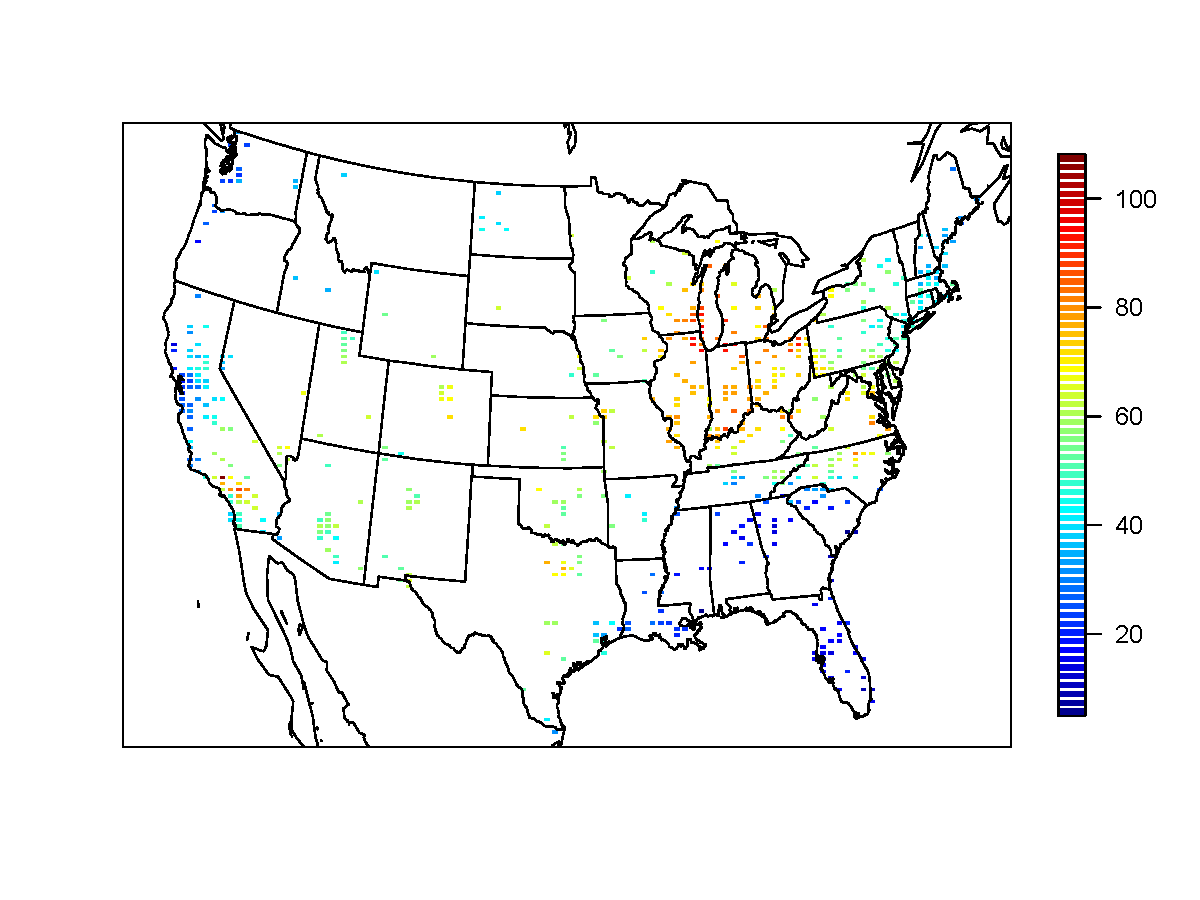
\includegraphics[width=0.75\linewidth]{plots/ozone-10jul-us.pdf}
  \caption{Ozone values (ppb) on July 10, 2005}
  \label{stfig:ozone-10jul}
\end{figure}

A spatial model for threshold exceedances warrants special consideration and standard spatial methods are likely to perform poorly.
First, because we are interested only in high values, we want to ``let the tail speak for itself''.
That is, if we fit a model to the entire data set, low-to-moderate values would influence the fit of the overall model.
As there are more of these values, they can unduly influence the distribution at the higher levels about which we are interested.
Our inference method will only use data which exceed a pre-selected threshold and will censor data below the threshold, thereby tailoring the fit to the levels of interest.
Second, likelihood-based spatial modeling typically assumes a Gaussian process, which is appropriate when mean behavior is of interest.
However, the Gaussian distribution is light-tailed and symmetric, and therefore may be inappropriate for modeling data which does not share this tail behavior.
Third, we aim to capture the dependence structure when ozone is at high levels, and dependence at these levels may not be well-represented by covariances which focus again on mean behavior.
Asymptotic dependence/independence (see \sref{sts:extdep}) are notions which describe how two random variables' probability of simultaneous exceedance of an extremely high level.
The Gaussian distribution always exhibits asymptotic independence, except in the case of perfect dependence, thus is an inappropriate model for data which exhibits asymptotic dependence.
To allow for more flexibility in the marginal tail and to allow for asymptotic dependence, the \skewt distribution forms the basis for our model.

Our approach differs from threshold modeling approaches based on extreme value distributions.
There has been extensive work on threshold modeling in the field of extreme value statistics where extreme events are naturally defined in terms of exceedances over a high threshold.
\citet{Davison1990} considered modeling threshold exceedances of univariate time series by the generalized Pareto distribution.
Threshold based inference for multivariate extreme value distributions was considered by \citet{Ledford1996} who introduced a censored approach that provides a way to deal with different types of exceedances of a threshold.
These models were extended to spatial models for threshold exceedances by \citet{Wadsworth2012} and \citet{Thibaud2013} who fit various models to spatial extremes using a censored pairwise likelihood \citep{Padoan2010} based on the approach of \citet{Ledford1996}.
\citet{Huser2014} further extended this to space-time modeling.
\citet{Wadsworth2014}, \citet{Engelke2015}, and \citet{Thibaud2013a} introduced more efficient inference for threshold exceedances of extremal spatial processes with full likelihood methods.
The previous approaches to threshold modeling are motivated by extreme value theory and assume the threshold is high enough that extremal models are valid for the data and for extrapolation beyond the range of observed values.
Moreover, these approaches are computationally intensive and limited to rather small datasets.
% For example, \citet{Wadsworth2014} present a simulation study with observations at 16 sites on a regular grid, and \citet{Engelke2015} analyze a dataset with observations at 35 meteorological stations.
Our application with ozone data does not fit into this framework because we do not focus on exceedances of a very high level, and we have observations at 1,089 ozone monitoring locations.

We propose a new spatiotemporal threshold exceedance model based on the \skewt process \citep{Padoan2011}.
We use a \skewt distribution because of its flexibility to model asymmetry and heavy-tailed data with the aim of modeling exceedances of a high fixed level at an unobserved location.
Our model allows for inference and predictions using the full likelihood with computing on the order of Gaussian models.
This allows us to use Bayesian methods, which we use to fit the model, handle censored data below the threshold, and make predictions at unobserved locations.
The multivariate skew normal distribution was introduced by \citet{Azzalini1996}, and this was extended to the multivariate \skewt by \citet{Branco2001}.
These skew-elliptical distributions have been used in the spatial setting \citep{Genton2004,Kim2004}.
\citet{Zhang2010} propose the skew-Gaussian process as a class of stationary processes that have skewed marginal distributions.
\citet{Padoan2011} examined the usage of skew-Gaussian and \skewt distributions for multivariate extremes.
In a spatial setting, the multivariate \skewt distribution demonstrates asymptotic dependence between observations at all sites regardless of the distance between the sites.
In order to address this concern, we introduce a random spatial partition similar to the method used by \citet{Kim2005} for non-stationary Gaussian data.
% This partitioning alleviates the asymptotic spatial dependence present in the \skewt distribution for sites that are far apart.

The paper is organized as follows.
\sref{sts:spatialskew} is a brief review of the spatial \skewt process.
In \sref{sts:spatial}, we build upon the traditional \skewt process by incorporating censoring, partitioning, and extending the model to space-time data.
The computing is described in \sref{sts:hier}.
In \sref{sts:simstudy}, we present a simulation study that examines the predictive capabilities of this model compared to Gaussian and max-stable methods.
We compare our method to Gaussian and max-stable methods with a data analysis of ozone measurements throughout the US in \sref{sts:analysis}.
% The final section provides brief discussion and direction for future research.

% These models describe dependence using the probability that two observations jointly exceed an extreme value, which in the limit of the distribution is referred to as asymptotic dependence.
% When the spatial domain is small, it may be reasonable to assume that all sites are asymptotically dependent; however for large spatial domains, it becomes more challenging to justify this assumption.
% This concern has been addressed by \citet{Wadsworth2012} in a spatial only setting and \citet{Huser2014} in a space-time setting.

% The main goal of our application is to estimate the marginal probability a site's ground-level ozone measurement will exceed 75 ppb.
% For July 2005, 75 ppb is approximately the 92nd sample quantile.
% However, if we look marginally at each site, 75 ppb is lower than the 90th quantile for almost 255 sites, and is below the median at 29 sites.
% The traditional threshold exceedance models arising from max-stable processes incorporate thresholding because the inference is only valid for very high values.
% Because 75 ppb represents such a wide range of marginal quantiles, these models based on max-stable methods may not be appropriate.

% Traditionally, spatial methods for extreme values analysis are conducted from one of two perspectives.
% The first of these is based on the convergence of the maximums of independent stochastic processes to a max-stable process \citep{deHaan2006}.
% Finite dimensional realizations of a max-stable process follow a generalized extreme value distribution \citep{Cooley2012}.
% One drawback to a block-maxima approach is that information is lost by discarding all but the most extreme observations in a block.
% Furthermore, in using multivariate block-maxima methods, the observations in the vector of block maxima rarely occur simultaneously \citep{Coles2001}.
% The other perspective incorporates a peaks-over-threshold approach.

% The use of multivarate models for threshold exceedances require evaluation of the underlying joint density.
% Finite dimensional realizations of max-stable processes are challenging to use because closed-form expressions for the density in more than two dimensions are complicated \citep{Coles1991}.
% One way to circumvent this challenge is to use pairwise composite likelihood methods \citep{Padoan2010}.
% When using pairwise composite likelihoods, threshold methods can then be implemented as long as the bivariate distribution can be evaluated \citep{Wadsworth2012,Thibaud2013,Huser2014}.
% Hierarchical models using Bayesian methods have also been proposed.
% For example, \citet{Reich2012} present a Bayesian hierarchical model, when conditioned on positive stable spatial random effects, the observations are independent.

% In certain settings, the multidimensional distributions are available.
% For example, \citet{Wadsworth2014} discuss a censored Poisson process that exploits the fact that the spectral functions for Brown-Resnick processes are log-Gaussian random fields.
% Additionally, \citep{Engelke2014}, show that upon standardizing marginals to the Gumbel distribution and conditioned on a fixed location exceeding a high threshold, the incremental distribution asymptotically forms a Gaussian process.
% In addition to Brown-Resnick processes, skew elliptical distributions can be used for multivariate modeling with dependent extreme values \citep{Genton2004,Zhang2010,Padoan2011}.
% For example, the skew-normal and \skewt distribution offer a flexible way to handle non-symmetric data within a framework of multivariate normal and multivariate $t$ distributions.
% As with multivariate Gaussian distributions, the multivariate skew-normal distribution demonstrates asymptotic independence. Conversely both the multivariate $t$ and \skewt distributions demonstrate asymptotic dependence \citep{Padoan2011}.
% Additionally, the limiting distribution of the maxima of \skewt random vectors is the extremal \skewt distribution \citep{Padoan2011} of which the extremal-$t$ \citep{Opitz2013} is a special case.

% Despite this challenge, spatial modeling is important because it provides a mechanism by which we can borrow information about extreme events across space.
% There are two primary goals for spatial methods.
% The first of these goals is to understand the marginal behavior at sites, and the second is to describe the dependence in the data.
% In many cases, these are done separately; however, with the development of pairwise composite likelihoods and Bayesian methods, it is resonable to model both simultaneously.
% One challenge to estimating the dependence in the tails of the distribution is that the dependence that present in the data may not be the same as the dependence in the limit of the underlying distribution \citep{Davison2012b}.
% Furthermore, in a spatial setting, it may be desirable to allow for varying degrees of tail dependence based upon the distance between two sites \citep{Wadsworth2012}.

\section{Spatial skew processes}\label{sts:spatialskew}
\sectionmark{Spatial skew processes}
The skew-elliptical family of distributions provides models that are mathematically tractable while introducing a slant parameter to account for asymmetric data.
A brief review of the additive process \citep[p. 129]{Azzalini2014} by which a \skewt process is created is given here.

\subsection{\Skewt process} \label{sts:skewt}
\subsectionmark{\Skewt process}
Let $Y(\bs)$ be a spatial process defined for spatial location $\bs$ in a spatial domain of interest $\calD \in \mathbb{R}^2$.
The spatial \skewt process can be written as
\begin{align}
  Y(\bs) = \bX(\bs)^\top \bbeta + \lambda \sigma |z| + \sigma v(\bs) \label{steq:fullmodel}
\end{align}
where $\bX(\bs)$ is the observed covariate vector at site $\bs$, $\bbeta$ is the $p$-vector of regression parameters, $\lambda \in \mathbb{R}$ is a parameter controlling skewness, $z \sim N(0, 1)$, $\sigma^2 \sim \mathrm{IG}(a / 2, b / 2)$ is random scale parameter, IG is the distribution function of an inverse gamma random variable, $a$ is the degrees of freedom, $b$ controls the precision of the process, and $v(\bs)$ is a standard Gaussian process with positive definite correlation function $\text{Cor} \left[Y(\bs_1), Y(\bs_2)\right] = \rho(\bs_1, \bs_2)$.
Although any positive definite correlation function could be used, we choose to use the stationary isotropic \Matern correlation with
\begin{align}
  \rho(h) = (1 - \gamma) I(h = 0) + \gamma \frac{ 1 }{ \Gamma(\nu) 2^{ \nu - 1}} \left( \sqrt{2\nu} \frac{ h }{ \varphi } \right)^{\nu} K_{\nu} \left( \sqrt{2\nu} \frac{ h }{ \varphi } \right) \label{steq:matern}
\end{align}
where $I(\cdot)$ is an indicator function, $\varphi > 0$ is the spatial range, $\nu > 0$ is the smoothness, $\gamma \in [0, 1]$ is the proportion of variance accounted for by the spatial variation, $K_\nu$ is a modified Bessel function of the second kind, and $h = || \bs_1 - \bs_2 ||$ is the Euclidean distance between sites $\bs_1$ and $\bs_2$.

For a finite collection of locations $\bs_1, \ldots, \bs_n$, we denote by $\bY = [Y(\bs_1), \ldots, Y(\bs_n)]^\top$ the vector of observations, and the covariate matrix $\bX_{n \times p} = [\bX(\bs_1), \ldots, \bX(\bs_n)]^\top$.
After marginalizing over both $z$ and $\sigma$, using the notation from \citet[p. 176]{Azzalini2014},
\begin{align} \label{steq:stazzalini}
  \bY \sim \text{ST}_n(\bX \bbeta, \bOmega, \balpha, a),
\end{align}
that is, $\bY$ follows an $n$-dimensional \skewt distribution with location $\bX \bbeta \in \mathbb{R}^n$; covariance matrix $\bOmega_{n \times n} = \bomega \left[ \frac{1}{1 + \lambda^2}(\bSigma + \lambda^2 \bOne \bOne^\top) \right] \bomega$, $\bSigma_{n \times n}$ is the positive definite correlation matrix which is obtained from $\rho(h)$, and $\bomega_{n \times n} = \text{diag}\left(\sqrt{\frac{ b }{a(1 + \lambda^2)}}, \ldots, \sqrt{\frac{ b }{a(1 + \lambda^2)}} \right)$; slant parameters $\balpha \in \mathbb{R}^n = \lambda (1 + \lambda^2)^{1 / 2} (1 + \lambda^2 \bOne^\top \bSigma^{-1} \bOne)^{-1/2} \bSigma^{-1} \bOne$, and degrees of freedom $a$.
Furthermore, the marginal distributions at each location also follow a univariate \skewt distribution \citep{Azzalini2014}.
This process is desirable because it is heavy tailed with tail index $a$, and the shape of the distribution is controlled by the skewness parameter.
% One major difference between the parameterization given in \eref{steq:fullmodel} and other parameterizations is that we characterize the skewnewss using $\lambda$ instead of the slant parameters $\balpha$.
For a comparison with other parameterizations, see \aref{sta:otherparams}.

% We use this parameterization for spatial correlation because the $\gamma$ parameter permits the inclusion of a nugget effect to account for non-spatial variability due to issues like measurement error.

\subsection{Extremal dependence}\label{sts:extdep}
\subsectionmark{Extremal dependence}
Our interest lies in spatial dependence in the tail of the \skewt process.
One measure of extremal dependence is the $\chi$ statistic \citep{Coles1999}.
For a stationary and isotropic spatial process, the $\chi$ statistic for two locations separated by distance $h$ is
\begin{align} \label{steq:chih}
  \chi(h) = \lim_{c \rightarrow c^*} \Pr[Y(\bs + h) > c | Y(\bs) > c]
\end{align}
where $c^*$ is the upper limit of the support of $Y$; for the \skewt distribution $c^* = \infty$.
If $\chi(h) = 0$, then observations are asymptotically independent at distance $h$.
For Gaussian processes, $\chi(h) = 0$ regardless of the distance $h$, so they are not suitable for modeling asymptotically dependent extremes.
Unlike the Gaussian process, the \skewt process is asymptotically dependent (the explicit expression for $\chi(h)$ is given in \aref{sta:skewt}).
However, one problem with the spatial \skewt process is that $\displaystyle \lim_{h \rightarrow \infty} \chi(h) > 0$.
This occurs because all observations, both near and far, share the same $z$ and $\sigma$ terms.
Therefore, this long-range dependence feature of the \skewt process is not desirable for spatial analysis of large geographic regions where we expect only local spatial dependence.
We propose a solution to this in \sref{sts:part}.

\section{Extending the model}\label{sts:spatial}
\sectionmark{Extending the model}
In this section, we propose extensions to the \skewt process to model spatial extremes over a large geographic region by introducing censoring to focus on tail behavior and a random partition to remove long-range asymptotic dependence.
For notational convenience, we introduce the model for a single replication, and then extend this model to the spatiotemporal setting in \sref{sts:temporal}.

\subsection{Censoring to focus on the tail} \label{sts:censoring}
We do not want the low-to-moderate values to influence the fit of the model.
We propose the use of a censored approach to fit threshold exceedances only.
More specifically, we assume our \skewt model $Y(\bs)$ is valid at each location $\bs$ above a threshold $T$, and censor the values below $T$ for which we don't assume the model to be valid.
We define our partially censored observations as $\widetilde{\bY} = [\widetilde{Y}(\bs_1), \ldots, \widetilde{Y}(\bs_n)]^\top$ where $\widetilde{Y}(\bs) = \max\{Y(\bs), T\}$, and fit the \skewt process to these $\widetilde{\bY}$.
In our Bayesian framework, inference can be easily performed by imputing censored observations below $T$ (see \sref{sts:comp}).
% We propose to use a censored approach because we do not want the low-to-moderate values to influence the fit of the model.
% % The censored observations below the threshold give information on the marginal probabilities to exceed the threshold and on the dependence, but their values are not used to fit the model.
% % \beq \label{steq:Yt}
% %   \widetilde{Y}(\bs) = \left\{ \begin{array}{ll}
% %       Y(\bs) \quad & \delta(\bs) = 1 \\
% %       T & \delta(\bs) = 0
% %   \end{array} \right.
% % \eeq
% We will assume our data were generated from the censored process $\widetilde{Y}(\bs) = \max\{Y(\bs), T\}$ where $T$ is a pre-specified threshold value.
% Then from the censored process, the vector of observations becomes $\widetilde{\bY} = [\widetilde{Y}(\bs_1), \ldots, \widetilde{Y}(\bs_n)]^\top$.

As our goal is to model exceedances above a high level $L$, we should select a value for $T \le L$.
For example, in predicting ozone exceedances, we might set $T = 50$ ppb in order to predict exceedances of $L = 75$ ppb.
Selecting $T$ too small may lead to bias in estimating the tail parameters; selecting $T$ too large increases variance.
We impute the censored values as a step in the algorithm used to fit the model described in \sref{sts:comp}, and use cross-validation to select $T$.

\subsection{Partitioning to remove long-range asymptotic dependence}\label{sts:part}
For a large spatial domain, it may not be reasonable to assume sites that are far apart demonstrate asymptotic dependence.%, so we handle the problem of long-range asymptotic dependence with a random partition.
% Modeling different levels of asymptotic dependence was discussed by \citet{Wadsworth2012}.
% \citet{Huser2014} also allow for varying asymptotic dependence across both space and time with a partition structure represented by random discs moving across the space for a random duration with a random velocity and random radius.
As discussed in \sref{sts:spatialskew}, the source of long-range dependence is the shared $z$ and $\sigma$.
Therefore, to alleviate this dependence, we allow $z$ and $\sigma$ to vary by site using a partitioning approach.
The model becomes
\begin{align} \label{steq:partition}
  Y(\bs) &= \bX(\bs)^\top \bbeta + \lambda \sigma(\bs) |z(\bs)| + \sigma(\bs) v(\bs).
\end{align}
To model spatial variation, consider a set of spatial knots $\bw_1, \ldots, \bw_K$ from a homogeneous Poisson process over spatial domain $\calD \in \mathbb{R}^2$.
The knots define a random partition of $\calD$ by subregions $P_{1}, \ldots, P_{K}$ defined as
\begin{align} \label{steq:subregions}
  P_{k} = \{ \bs : k = \argmin_\ell || \bs - \bw_{\ell} || \}.
\end{align}
In other words, $P_k$ is composed of all sites for which the closest knot is $\bw_k$.
For all $\bs \in P_k$, with $k = 1, 2, \ldots, K$, the functions $z(\bs)$ and $\sigma(\bs)$ are equal to the constants $z_k$ and $\sigma_k$ respectively, and the $z_k$ and $\sigma^2_k$ are distributed as $z_k \iid N(0, 1)$ and $\sigma^2_k \iid \mathrm{IG}(a / 2, b / 2)$.
So, within each partition, $Y(\bs)$ follows the spatial \skewt process defined in \sref{sts:spatialskew}.
Across partitions, the $Y(\bs)$ remain dependent via the correlation function for $v(\bs)$ because $v(\bs)$ spans all partitions.
However, the bivariate distribution for sites in different partitions is neither Gaussian nor \skewt and does not have asymptotic dependence.

The partitioning model removes long-range dependence.
Conditional on knots $\bw_1, \ldots, \bw_K$, the $\chi$ statistic for two sites $\bs_1$ and $\bs_2$ in partitions $k_1$ and $k_2$ respectively is
\begin{align}
  \chi(h) &= I(k_1 = k_2) \chi_{\text{skew-}t}(h) \label{steq:chiskewt}
\end{align}
where $\chi_{\text{skew-}t}(h)$ is the $\chi$ statistic for a \skewt process given in equation \eref{steq:chiskew-t} of \aref{sta:skewt}, and $h = ||\bs_1 - \bs_2||$.
Marginally, over the knots, $\chi(h) = \pi(h) \chi_{\text{skew}-t}(h)$, where \mbox{$\pi(h) = \Pr(k_1 = k_2)$} is the probability that two sites separated by distance $h$ are in the same partition.
In \aref{sta:proofsamepartition}, we show that assuming the knots follow a homogeneous Poisson process, $\displaystyle \lim_{h \rightarrow \infty} \pi(h) = 0$, and thus long-range dependence is removed.
% In \aref{sta:proofsamepartition}, we show that $\lim_{h \rightarrow \infty} \pi(h) = 0$, assuming that the knots follow a homogeneous Poisson process.
% This implies that $\lim_{h \rightarrow \infty} \chi(h) = 0$.
In practice we fix $K$ at a finite value and use a uniform distribution for the knots $\bw_1, \ldots, \bw_K$.
In \fref{stfig:chi}, we estimate $\chi(h)$ for $K = 1, 3, 5, 10$ partitions for a \skewt distribution with $\alpha = 10$, and 3 degrees of freedom.
% In \fref{stfig:chi} we estimate $\pi(h)$ through simulation.
% To estimate $\pi(h)$, we generate 500 sites uniformly over the unit-square.
% We then randomly generate 400 different sets of partitions using $K = 3$, $5$, and $10$.
% For each set of knots, we take $\pi(h)$ to be the proportion of sites in the same partition that are separated by distance $h$.
% This plot demonstrates how partitioning helps to reduce extremal dependence as $h$ increases.
\begin{figure}
  \centering
  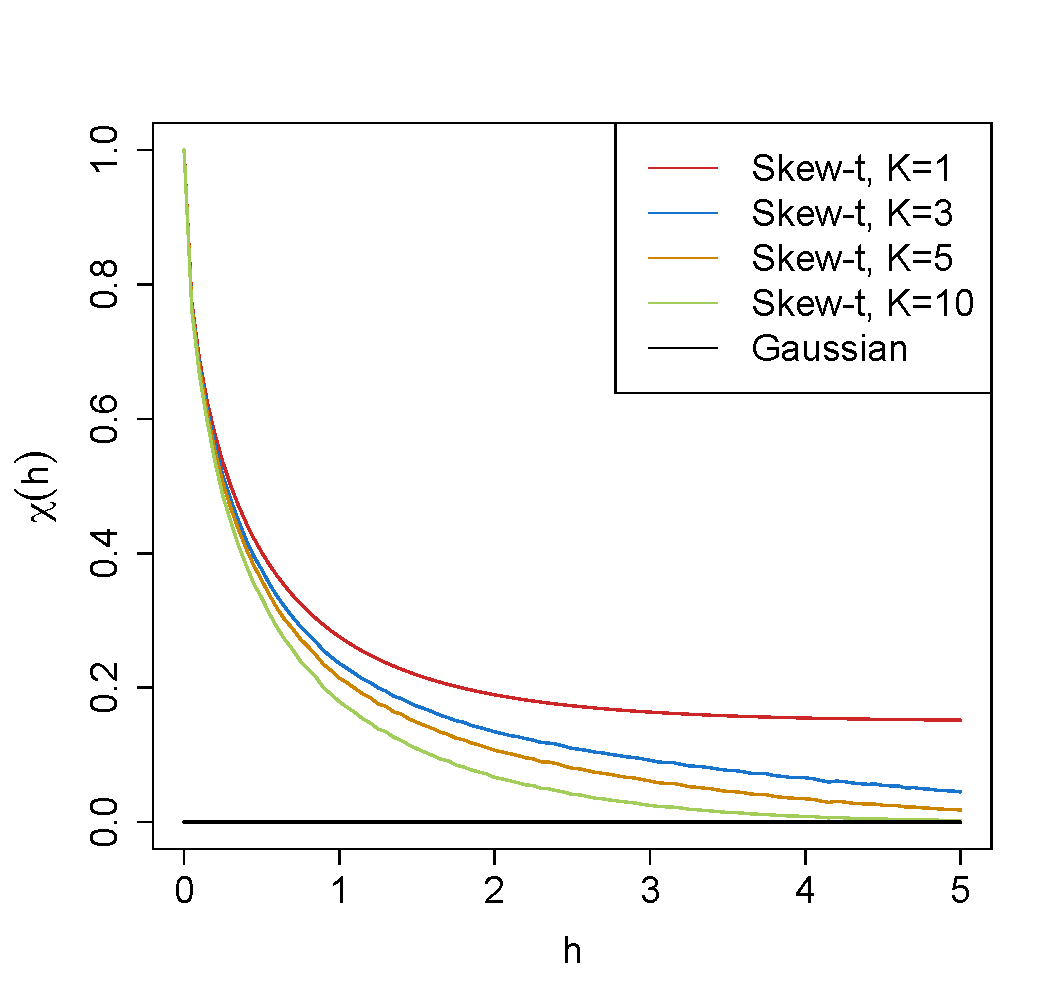
\includegraphics[width=0.5\linewidth]{plots/chi-h.pdf}
  \caption{Extremal dependence measure $\chi(h)$, as a function of distance, $h$, for $K = 1, 3, 5$, and $10$ knots.}
  \label{stfig:chi}
\end{figure}

\subsection{Extension to space-time data} \label{sts:temporal}
When using daily measurements, the assumption of temporal independence is often inappropriate.
In this section, we extend \eref{steq:partition} to the spatiotemporal setting.
There are several places where temporal dependence could be incorporated in the model, including the Gaussian process $v_t(\bs)$.
However, we choose to allow for temporal dependence in the $\bw$, $z$, and $\sigma$ terms because these terms dictate the tail behavior of the process which is our primary focus (see \aref{sta:temporal} for a discussion of the induced temporal asymptotic dependence).
Let
\begin{align} \label{steq:spatiotemp}
  Y_t(\bs) = \bX_t(\bs)^\top \bbeta + \lambda \sigma_t(\bs) |z_t(\bs)| + \sigma_t(\bs) v_t(\bs),
\end{align}
where $t \in \{1, \ldots, n_t\}$ denotes the day of each observation.
Let \hbox{$\bw_{tk} = (w_{tk1}, w_{tk2})$} be a spatial knot on day $t$, and let $\bw_{t1}, \ldots, \bw_{tK}$ be the collection of spatial knots on day $t$.
As in \sref{sts:part}, these knots define a daily partition $P_{t1}, \ldots, P_{tK}$, and for $\bs \in P_{tk}$,
\begin{align}
  z_t(\bs) = z_{tk}\quad \text{and} \quad \sigma_{t}(\bs) = \sigma_{tk}.
\end{align}
We allow the partition structure to vary from day to day in order to account for sharp spikes in a response that may not be present every day (e.g. the impact of a forest fire on ozone levels).

We use an AR(1) time series model for $\bw_{tk}$, $z_{tk}$, and $\sigma_{tk}$.
The time series model must be specified after a transformation to preserve the \skewt process at each time point.
For each time-varying parameter, we transform the parameter to obtain a standard normal marginal distribution, place a Gaussian prior with autocorrelation on the transformed parameter, and then transform back to the appropriate marginal distribution for the \skewt process.
We first transform the spatial knots from $\calD$ to $\mathbb{R}^2$ as follows.
Let
\begin{align} \label{steq:wstar}
  w^*_{tki} = \Phi^{-1}\left[ \frac{ w_{tki} - \min(\bs_i)}{ \max(\bs_i) - \min(\bs_i) } \right], \quad i = 1, 2
\end{align}
where $\Phi$ is a univariate standard normal density function and $\bs_i = [s_{1i}, \ldots, s_{ni}]$.
Then the transformed knots $\bw^*_{tk} \in \mathbb{R}^2$.
We use a transformation of a Gaussian random variable on $z_{t}(\bs)$ to ensure that the marginal distributions of $z_t(\bs)$ are half-normal.
Let
\begin{align} \label{steq:zstar}
  z^*_t(\bs) = \Phi^{-1}\left\{ \text{HN}[z_t(\bs)] \right\}
\end{align}
where HN is the distribution function of a half-normal random variable.
We also use a transformation of a Gaussian random variable on $\sigma^2_t(\bs)$ to ensure that the marginal distributions of $\sigma^2_t(\bs)$ are inverse gamma.
Let
\begin{align} \label{steq:sigmastar}
  \sigma^{2*}_t(\bs) =\Phi^{-1}\left\{ \text{IG}[\sigma^2_t(\bs)] \right\}
\end{align}
where IG is defined as before.
The AR(1) process for each tail parameter is $\bw^*_{1k} \sim N_2(\bZero, \bI_2)$ where $\bI_2 = \text{diag}(1, 1)$, $z^*_{1k} \sim N(0, 1)$, $\sigma^{2*}_{1k} \sim N(0, 1)$, and for $t > 1$ the time series is modeled as
\begin{align}
  \bw^*_{tk} | \bw^*_{t-1, k} &\sim N_2\left[\phi_w \bw^*_{t-1, k}, (1 - \phi_w^2) \bI_2 \right] \label{steq:ts-wstar}\\
  z^*_{tk} | z^*_{t-1, k} &\sim N \left[\phi_z z^*_{t-1, k}, (1 - \phi_z^2)\right] \label{steq:ts-zstar} \\
  \sigma^{2*}_{tk} | \sigma^{2*}_{t-1, k} &\sim N \left[\phi_\sigma \sigma^{2*}_{t-1, k}, (1 - \phi_\sigma^2) \right] \label{steq:ts-sigmastar}
\end{align}
where $|\phi_w|$, $|\phi_z|$, $|\phi_\sigma| < 1$.
These are stationary time series models with marginal distributions \hbox{$\bw^*_{k} \sim N_2(\bZero, \bI_2)$} \hbox{$z^*_{k} \sim N(0, 1)$}, and \hbox{$\sigma^{2*}_{k} \sim N(0, 1)$}.
After transformation back to the original space, $\bw_{tk} \sim \mathrm{Unif}(\calD)$, $z_{tk} \sim \mathrm{HN}(0, 1)$, and $\sigma^2_{tk} \sim \mathrm{IG}(a / 2, b / 2)$.
We then create the partition for day $t$ using $\bw_{t1}, \ldots, \bw_{tK}$.
For each day, the model is identical to the spatial-only model in \eref{steq:partition} by construction.

\section{Hierarchical model}\label{sts:hier}
We define a Bayesian hierarchical model based on the \skewt process and use a Markov chain Monte Carlo (MCMC) algorithm to fit the data.
We model our data as partially censored observations (see \sref{sts:censoring}) from the \skewt model defined in \sref{sts:spatial}.
In the first step of the MCMC algorithm, we impute censored values of $\widetilde{Y}$ such that the estimation of model parameters can be based on the completed $\bY$.
% We model our data as observations from the censored \skewt model defined in \sref{sts:censoring}.
Conditioned on $z_{tk}(\bs)$, $\sigma^2_{tk}(\bs)$, and $P_{tk}$, joint distribution of $\bY$ is multivariate Gaussian.
We do not fix the partitions; instead, the locations of the $K$ knots are treated as unknown and random.
% The first step in the algorithm is to update the knot locations, $z_{tk}(\bs)$, $\sigma^2_{tk}(\bs)$.
% The knot locations are treated as unknown and random in the MCMC algorithm.
% For level
%  $\bw_{t1}, \ldots, \bw_{tK}$ be a set of daily spatial knots in a spatial domain of interest, $\calD$, and $P_{tk}$ as defined in \eref{steq:subregions}.
One approach would be to allow $K$ to be unknown and follow a Poisson process prior, but this would lead to onerous computing.
Therefore, we elect to treat $K$ as a tuning parameter for the MCMC by fixing it at different values and assessing its impact on prediction as described in \sref{sts:modelselect}.
Then the hierarchical model is given as
\begin{align}
   Y_t(\bs) \mid z_{t}(\bs), \sigma_t^2(\bs), P_{tk}, \Theta &= \bX_t(\bs)^\top \beta + \lambda \sigma_t(\bs) |z_t(\bs)| + \sigma_t(\bs) v_t(\bs) \label{steq:hier}\\
   z_t(\bs) &= z_{tk} \text{ if } \bs \in P_{tk}\nonumber\\
   \sigma^2_{t}(\bs) &= \sigma^2_{tk} \text{ if } \bs \in P_{tk}\nonumber\\
   \lambda & \sim N(0, \sigma^2_\lambda)\nonumber \\
   % \lambda_1 &= \left\{ \begin{array}{ll}
   %    +1 \quad & \text{w.p. } 0.5\\
   %    -1 \quad & \text{w.p. } 0.5
   % \end{array}\right.\nonumber\\
   % \lambda^2_2 & \sim IG(a, b)\nonumber\\
   v_t(\bs) \mid \Theta &\sim \Matern(\bZero, \bSigma)\nonumber
\end{align}
% \begin{align*}
%    z^*_{tk} \mid z^*_{t-1, k} &\sim N(\phi_z z^*_{t-1, k}, (1 - \phi_z^2))\nonumber\\
%    \sigma^{2*}_{tk} \mid \sigma^{2*}_{t-1, k} &\sim N(\phi_\sigma \sigma^{2*}_{t-1, k}, (1 - \phi_\sigma^2))\nonumber\\
%    \bw^*_{tk} \mid \bw^*_{t-1, k} &\sim N_2(\phi_w \bw^*_{t-1, k}, \bI_2 (1 - \phi_w^2) ) \nonumber
% \end{align*}
where $\Theta = \{\varphi, \nu, \gamma\, \lambda, \bbeta\}$, $\bSigma$ is a \Matern covariance matrix as described in \sref{sts:skewt}, and the priors on $\bw^*_{tk}$, $z^*_{tk}$, and $\sigma^{2*}_{tk}$ are given in \eref{steq:ts-wstar} -- \eref{steq:ts-sigmastar}.

\subsection{Computation}\label{sts:comp}
We use MCMC methods to estimate the posterior distribution of the model parameters.
At each MCMC iteration, we first impute values below the threshold conditional on observations above the threshold.
% This is feasible for large datasets with our model because for a single day, conditional on the model parameters, we only need to draw from a truncated multivariate normal distribution.
% We can use Gibbs sampling to update $Y_t(\bs)$ for censored observations that are below the threshold $T$.
After conditioning on $\lambda$, $z_t(\bs)$ and non-censored observations, $Y_t(\bs)$ has truncated normal full conditionals $Y_t(\bs) \sim N_{(-\infty, T)}(\bX_t^\top(\bs) \beta + \lambda | z_t(\bs)|, \bSigma)$.

We update model parameters $\Theta$ using Gibbs sampling with Metropolis-Hastings steps when needed.
In our case, we also wish to be able to make predictions at sites where we do not have data.
We can easily implement Bayesian Kriging as a part of the algorithm to generate a predictive distribution for $Y_t(\bs^*)$ at prediction location $\bs^*$.
This step is similar to the imputation for censored observations except that the full conditionals are no longer truncated at $T$.
See Appendices A.1 and A.2 for details regarding the MCMC algorithm.

\section{Simulation study}\label{sts:simstudy}
In this section, we present the results from a simulation study to investigate how the number of partitions and the amount of thresholding impact the accuracy of predictions made by the model and to compare with Gaussian and max-stable methods.

\subsection{Design}\label{sts:simdesign}
For all simulation designs, we generated data from model \eref{steq:partition} in \sref{sts:part} using $n_s=144$ sites and $n_t=50$ independent days.
The sites were generated uniformly on the square $[0, 10] \times [0, 10]$.
We generated data from five different simulation designs:
\begin{enumerate}
  \item Gaussian, $K=1$ knot
  % \item Symmetric-$t$ marginal, $K=1$ knot
  % \item Symmetric-$t$ marginal, $K=5$ knots
  \item \Skewt, $K=1$ knots
  \item \Skewt, $K=5$ knots
  \item \citet{Reich2012} max-stable process %with GEV(1, 1, 0.2) marginals with dependence parameteter $\gamma_{\text{AL}} = 0.5$
  % \item Transformation below $T = q(0.80)$
  \item Brown-Resnick max-stable process \citep{Kabluchko2009} %with unit Fréchet marginals and stable semivariogram with range 1 and smoothness 0.5
\end{enumerate}
In the first three designs, the realizations from $v_t(\bs)$ were generated using a \Matern covariance with smoothness parameter $\nu = 0.5$, spatial range $\varphi = 1$ and $\gamma = 0.9$.
In the first design, $\sigma^2 = 2$ was used for all days which results in a Gaussian distribution.
For designs 2 and 3, $\sigma^2_{tk} \iid \text{IG}(3, 8)$ to give a $t$ distribution with 6 degrees of freedom.
For design 1, we set $\lambda = 0$.
For designs 2 and 3, $\lambda = 3$ was used as to simulate moderate skewness, and the $z_t$ were generated as described in \sref{sts:part}.
In designs 1 -- 3, the mean $\bX^\top \bbeta = 10$ was assumed to be constant across space.
In the fourth design, we generated from the max-stable model of \citet{Reich2012}.
The marginal distributions follow a generalized extreme value distribution with location parameter 1, scale parameter 1, and shape parameter 0.2.
Spatial dependence in the form an asymmetric logistic dependence function is induced by random effects for kernel basis functions associated with 144 spatial knots defined on a square grid on $[1,9] \times [1,9]$.
We set the dependence parameter ($\alpha$ in Reich and Shaby, 2012) to 0.5 which represents moderate spatial dependence.
For the final design, we generated data from a Brown-Resnick max-stable process  using \texttt{rmaxtab} in the \texttt{SpatialExtremes} package of \texttt{R} \citep{Ribatet2015}.
For this design we fixed unit \Frechet margins, and we used a range of 1 and smoothness 0.5.
% In the final design, we generate $\tilde{y}$ using the setting from design 2, and then transform the data
% \begin{align}
%   y = \left\{ \begin{array}{lc}
%     \tilde{y}, \quad & \tilde{y} > T \\[0.5em]
%     T \exp\{\tilde{y} - T\}, \quad & \tilde{y} \le T
%   \end{array}\right.
% \end{align}
% where $T = q(0.80)$ is the 80th sample quantile of the data.
% The final design is included to explore the importance of using a threshold exceedance model when the distribution for the bulk of the data is misspecified.

$M = 50$ data sets were generated for each design.
For each data set we fit the data using six models
\begin{enumerate}
  \item Gaussian marginal, $K=1$ knots
  \item \Skewt marginal, $K=1$ knots, $T=-\infty$
  \item Symmetric-$t$ marginal, $K=1$ knots, $T=q(0.80)$
  \item \Skewt marginal, $K=5$ knots, $T=-\infty$
  \item Symmetric-$t$ marginal, $K=5$ knots, $T=q(0.80)$
  \item \citet{Reich2012} max-table model thresholded at $T = q(0.80)$
\end{enumerate}
where $q(0.80)$ is the 80th sample quantile of the data.
All methods were fit using a fully-Bayesian approach that simultaneously estimates marginal and spatial dependence parameters.
The design matrix $\bX$ includes an intercept with a first-order spatial trend with priors of $\beta_\text{int}$, $\beta_\text{lat}$, $\beta_\text{long},  \iid \text{N}(0, 10)$ although only the intercept is used in the data generation.
The spatial covariance parameters have priors $\log(\nu) \sim \text{N}(-1.2, 1)$, $\gamma \sim \text{Unif}(0, 1)$, $\varphi \sim \text{Unif}(0, 15)$.
The skewness parameter has prior $\lambda \sim N(0, 20)$.
The residual variance terms have priors $\sigma^2_t(\bs) \sim \text{IG}(a / 2, b / 2)$, where $a$ has a discrete uniform prior on a mesh from $0.2$ to $20$ with spacing of $0.1$ and $b$ has a Gamma$(0.1, 0.1)$ prior.
As described in \sref{sts:skewt}, these priors are meant to be fairly uninformative to allow the data to dictate both the degrees of freedom $a$ and precision $b$ of the process.
The knots have priors $\bw \sim \text{Unif}(\calD)$.
We tried also fitting the \skewt marginals for the thresholded models, but it is very challenging for the MCMC to properly identify the skewness parameter with a censored left tail.
Each chain of the MCMC ran for 20,000 iterations with a burn-in period of 10,000 iterations.
Although the goal of this simulation study is not to assess parameter estimation, for design (2) and method (2) where data are generated and fit with a \skewt distribution, the samples converges for $\lambda$ and $a$, and the empirical coverage of posterior 95\% intervals is near the nominal level (96\% coverage for $\lambda$ and 90\% for $a$).
It should be noted that in the models with multiple partitions (i.e. models 4 and 5) it is hard to assess the convergence of $\bw$, $z(\bs)$, and $\sigma^2(\bs)$ because of partition label switching throughout the MCMC; however, we are not interested in these parameters but rather spatial predictions and tail probabilities which converge well.
Finally, we did not fit a Brown-Resnick model because we cannot use a Bayesian approach with so many sites.

\subsection{Cross validation}\label{sts:modelselect}
Models were compared using cross validation, with 100 sites used as training sites to fit the models, and 44 sites withheld for testing the predictions.
Because one of the primary goals of this model is to predict exceedances over a high level, we use Brier scores to compare the models \citep{Gneiting2007}.
The Brier score for predicting exceedance of a level $L$ is given by $[e(L) - P(L)]^2$ where $e(L) = I[y>L]$ is an indicator function indicating that a test set value, $y$, has exceeded the level, $L$, and $P(L)$ is the predicted probability of exceeding $L$.
We average the Brier scores over all test sites and days.
For the Brier score, a lower score indicates a better fit.

\subsection{Results}\label{sts:simresults}
We compared the Brier scores for exceeding four different high levels for each dataset.
The levels used for the Brier scores are extreme quantiles from the simulated data for $L = q(0.90)$, $q(0.95)$, $q(0.98)$, $q(0.99)$.
\fref{stfig:simbrierscores} gives the Brier score relative to the Brier score for the Gaussian method calculated as
\begin{align}
  \text{BS}_{\text{rel}} = \frac{\text{BS}_{\text{method}}}{\text{BS}_{\text{Gaussian}}}.
\end{align}
We analyzed the results for the simulation study using a Friedman \citep{Hollander2014} test at $\alpha = 0.05$ to see if at least one method had a significantly different Brier score.
For Friedman tests that came back with a significant p-value, we conducted a Wilcoxon-Nemenyi-McDonald-Thompson \citep{Hollander2014} test to see which of the methods had different results.
The full results for the Wilcoxon-Nemenyi-McDonald-Thompson tests are given in \aref{sta:pdiffs}.

In general, we find that when the method to fit the data matches the data generation scheme, there is some improvement over other methods.
The results show that when the data are generated from a Gaussian process, our method performs comparably to a Gaussian approach.
In general, when the underlying process is not Gaussian, our method results in an improvement over both the max-stable and Gaussian methods.
We also see that the non-thresholded methods tend to outperform the thresholded methods, but this is not surprising given that in most cases, the data are generated directly from the model.
Finally, in the case where the data are generated from a Brown-Resnick process, we find that our method is competitive with using a max-stable model.
% Finally, for setting 5, although the thresholded version of the single-partition model tends to perform the best across all of the extreme quantiles, the difference between the thresholded and non-thresholded methods is no longer significant in the more extreme quantiles.
In summary, our method provides great flexibility for data that demonstrate some level of asymmetry and heavy tails, while still performing comparably to Gaussian methods when the data are symmetric and have light tails.

\begin{figure}
  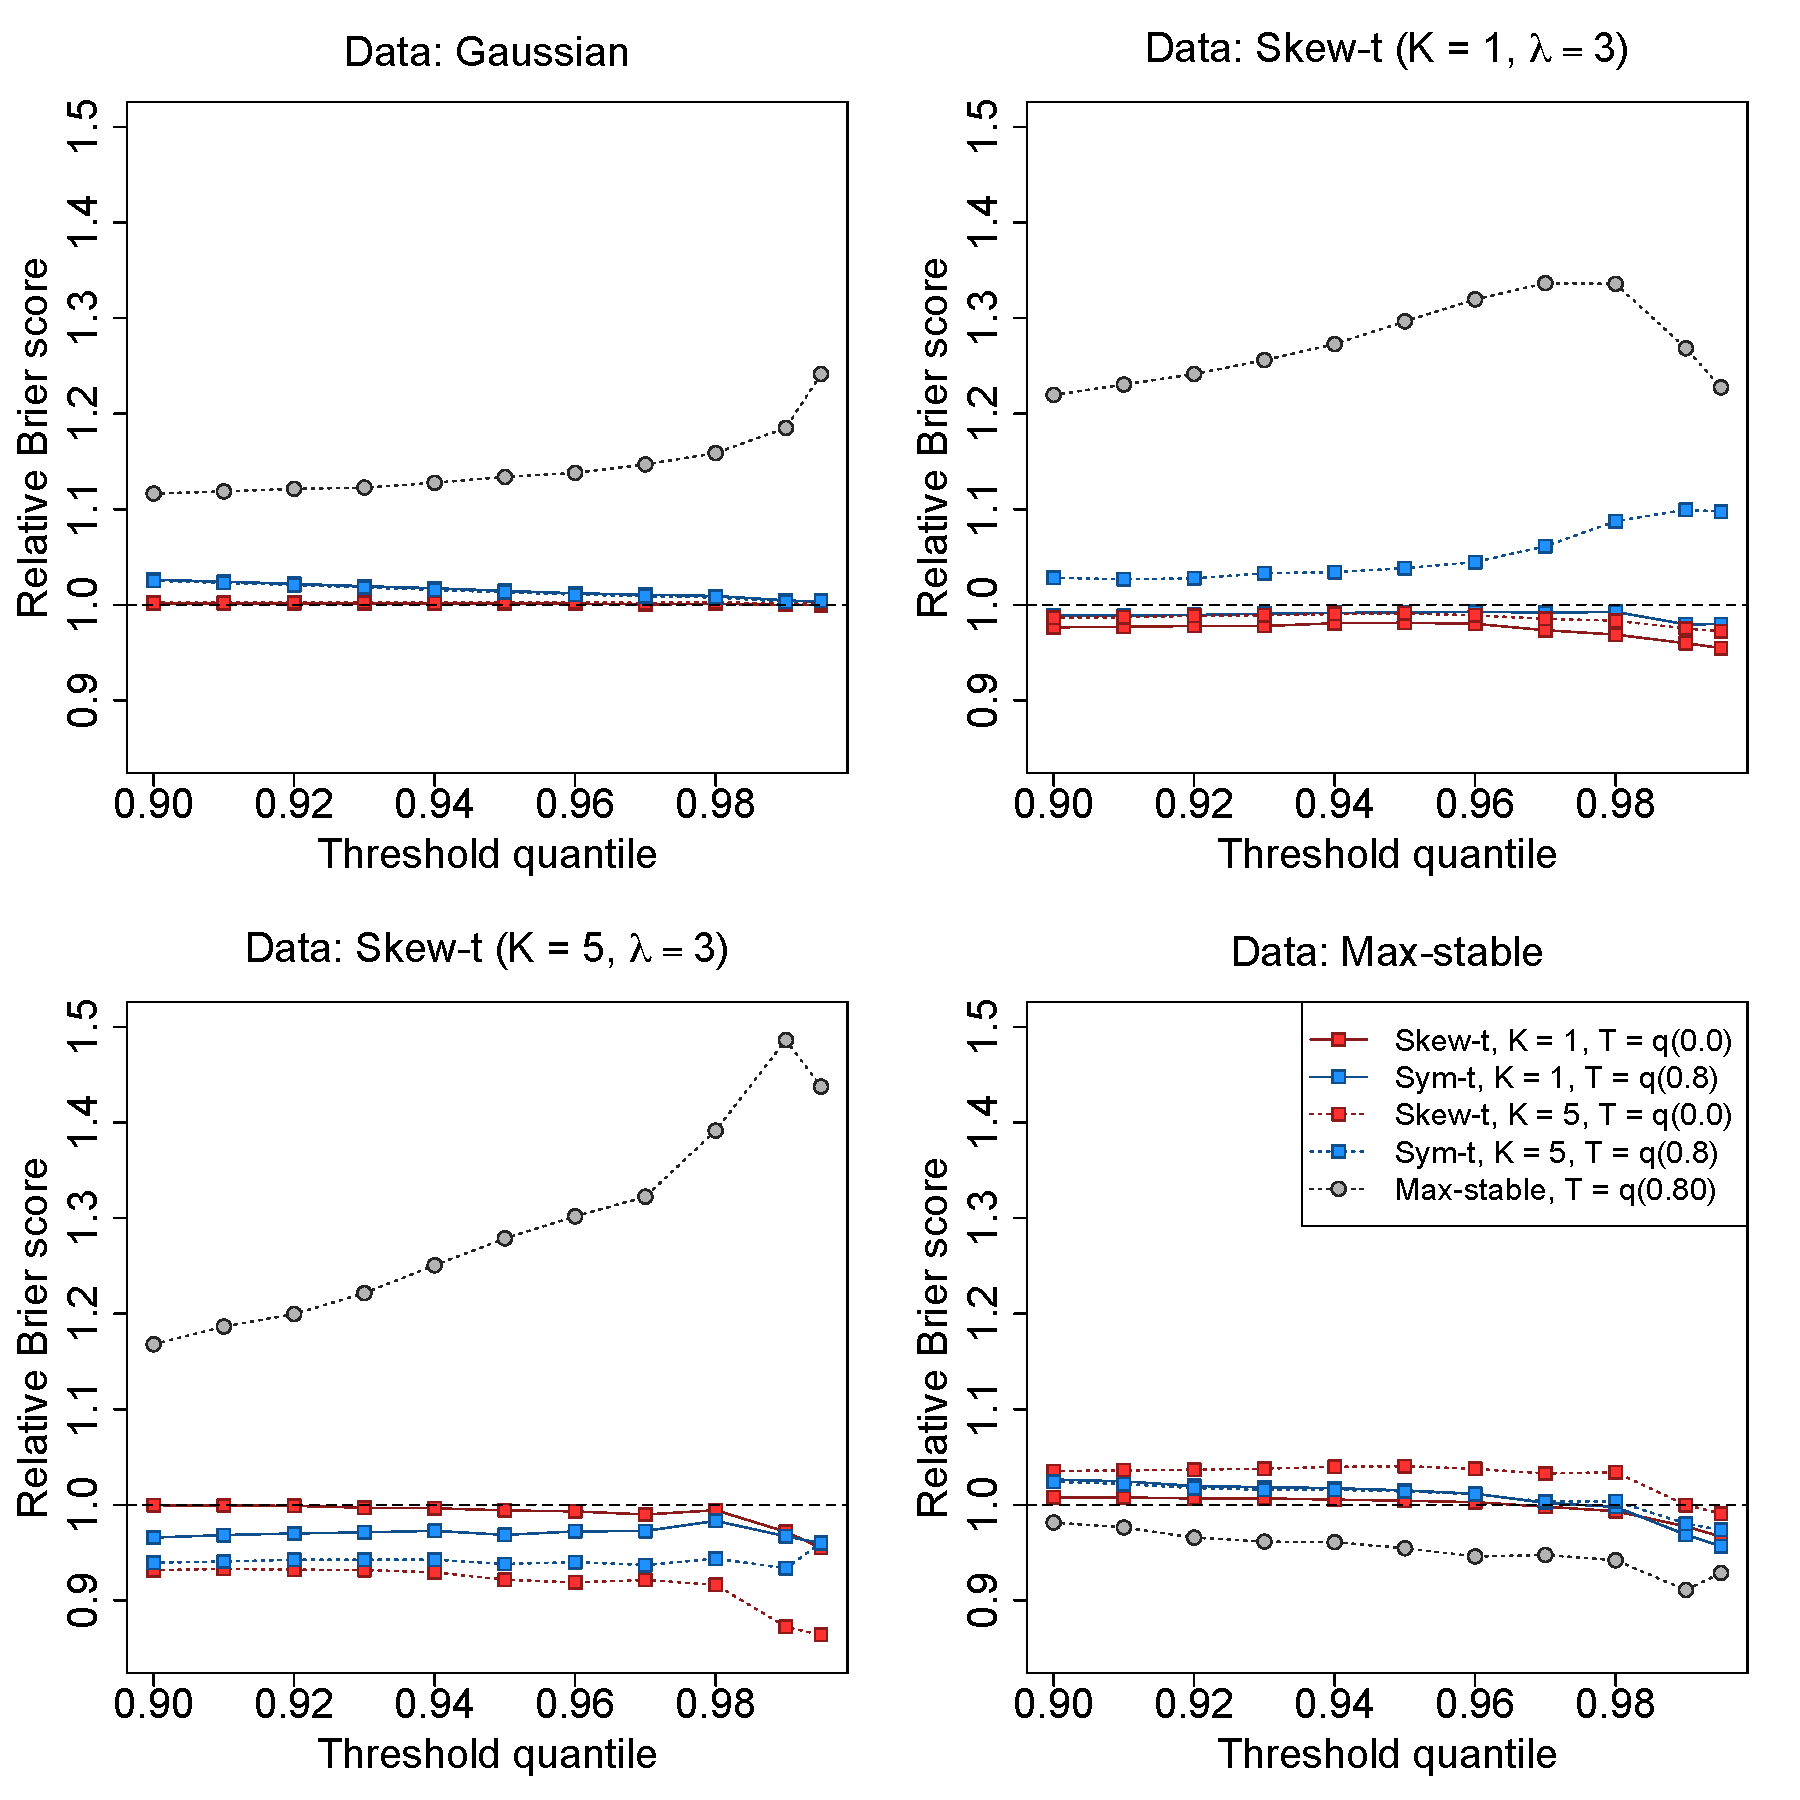
\includegraphics[width=\linewidth]{plots/bsplots-mean.pdf}
  \caption{Brier scores relative to the Gaussian method for simulation study results. A ratio lower than 1 indicates that the method outperforms the Gaussian method.}
  \label{stfig:simbrierscores}
\end{figure}

\section{Data analysis}\label{sts:analysis}
We consider daily observations of maximum 8-hour ozone measurements for the 31 days of July 2005 at 1,089 Air Quality System (AQS) monitoring sites in the United States as the response (see \fref{stfig:ozone-10jul}).
For each site, we also have covariate information containing the estimated ozone from the Community Multi-scale Air Quality (CMAQ) modeling system.
Initially, we fit a linear regression with $\bX_t(\bs) = [1, \text{CMAQ}_t(\bs)]^\top$. % assuming a mean function of
% \begin{align}
%   \text{E}[Y_i(\bs)] = \beta_0 + \beta_1 \cdot \text{CMAQ}_t(\bs). \label{steq:datamean}
% \end{align}
\fref{stfig:ozone-qq} shows a Q-Q plot of the residuals compared to a \skewt distribution with $a = 10$ and $\lambda = 1$, suggesting the data are heavy tailed.
\begin{figure}
  \centering
  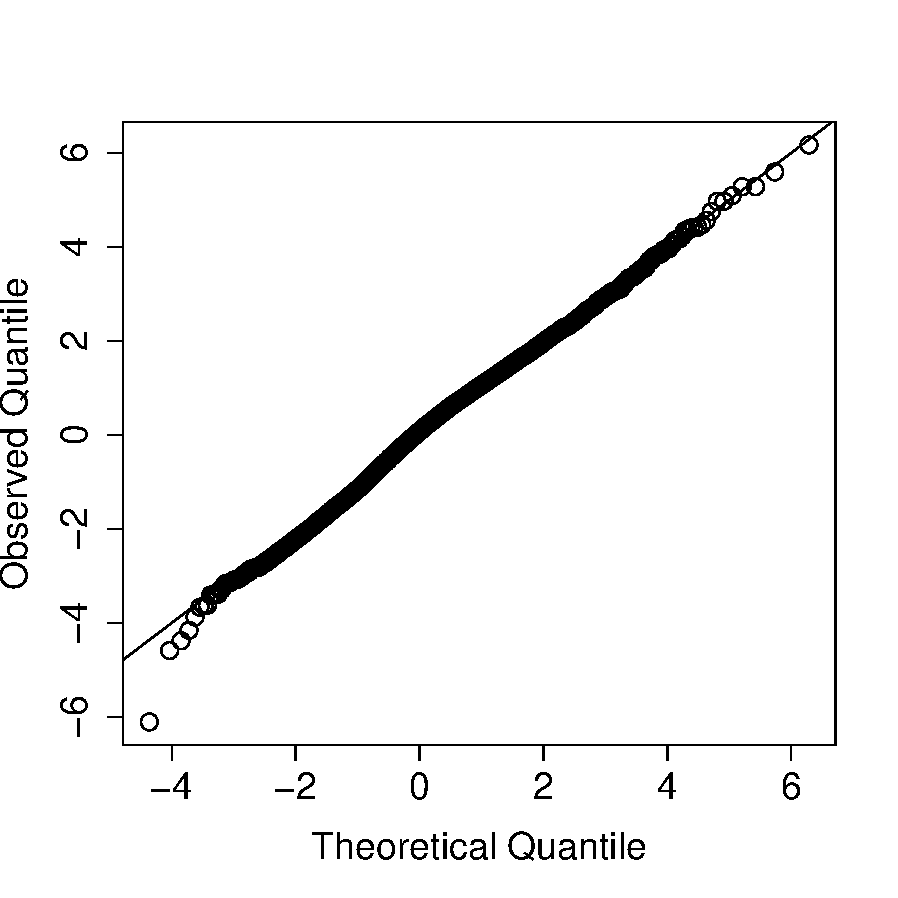
\includegraphics[width=\linewidth]{plots/qq-res.pdf}
  \caption{Gaussian Q-Q plot (left) and \skewt with $a = 10$ and $\lambda = 1$ Q-Q plot (right) of the residuals.}
  \label{stfig:ozone-qq}
\end{figure}

Standard exploratory data analysis techniques for extremal dependence are very challenging with only 31 days worth of data because it is difficult to estimate extreme quantiles at each site to obtain empirical estimates of $\chi$.
Despite the fact that there is only one month of data, we can get some sense of extremal dependence between sites by looking at joint occurrences of high sample quantiles.
For example, \fref{stfig:bivariateozone} suggests there is more agreement between sites that are close to one another than sites that are far from one another.
\begin{figure}
  \centering
  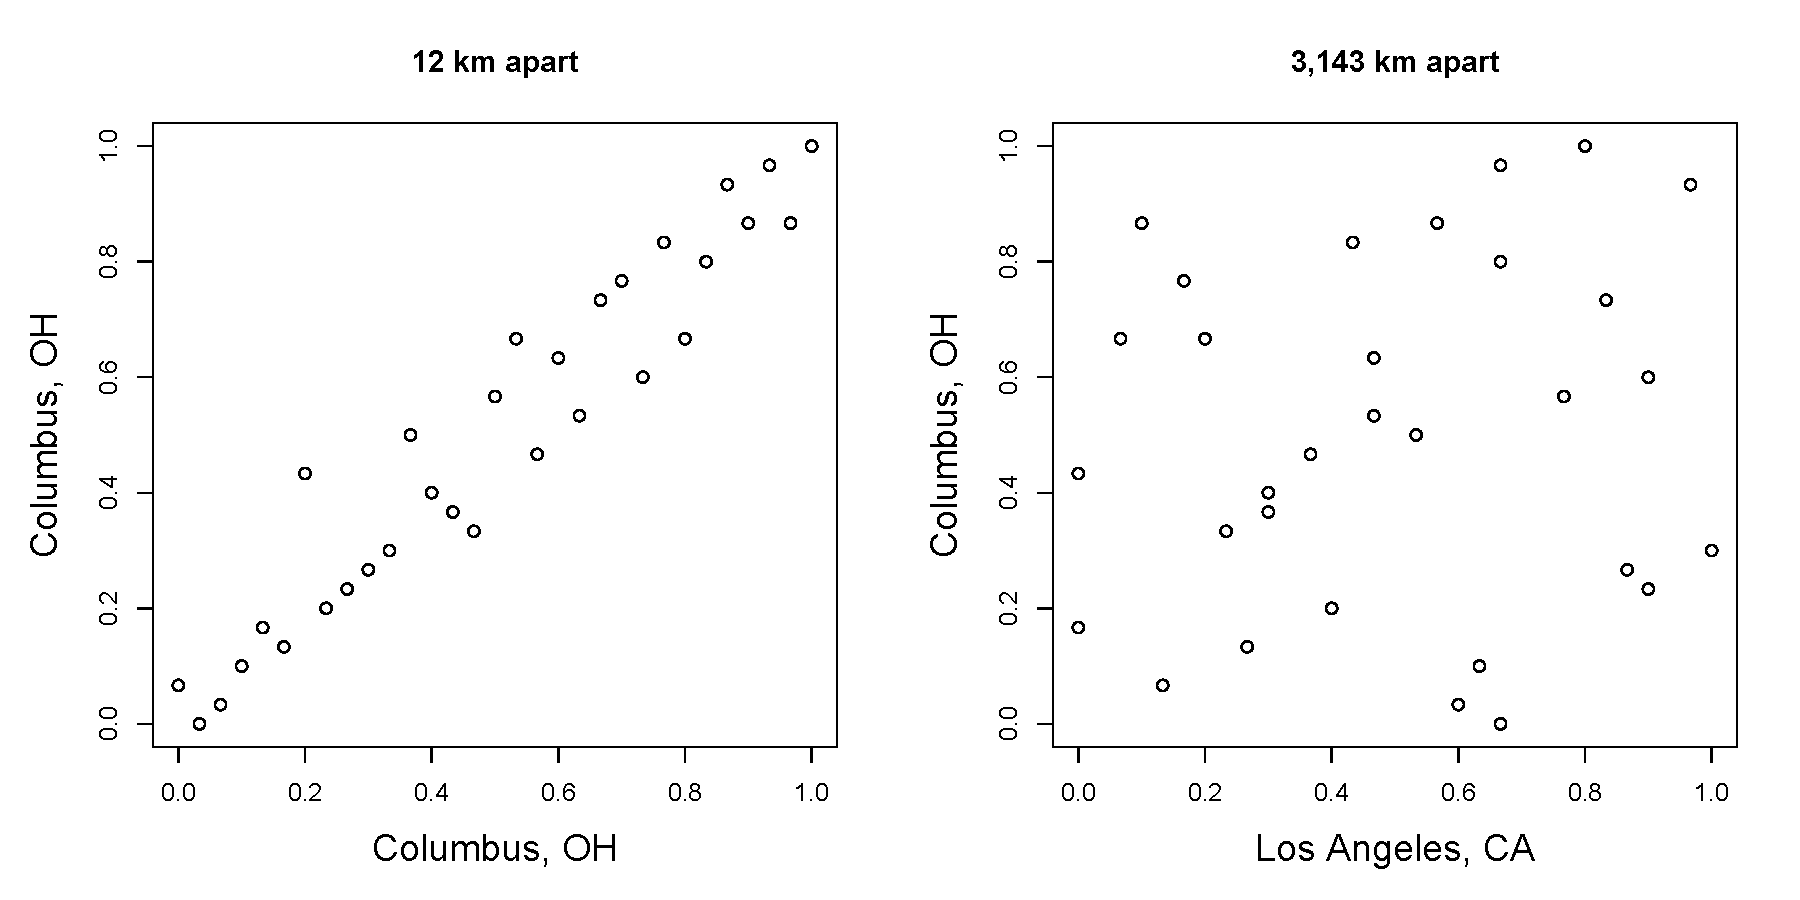
\includegraphics[width=\linewidth]{plots/daily-quantiles-ozone.pdf}
  \caption{Daily quantiles for two monitoring locations near Columbus, OH (left) and daily quantiles for a monitoring location in Los Angeles, CA and Columbus, OH (right)}
  \label{stfig:bivariateozone}
\end{figure}
% Another aspect that distinguishes our approach from more traditional extremes analyses, is how the threshold is selected.
% In our example, a threshold of 75 ppb which corresponds to $q(92)$ for all observations, but marginally it represents anywhere from $q(0.06)$ to $q(1)$.

% We explore spatial and temporal extremal dependence by considering $\chi_c = \Pr[Y(\bs) > c | Y(\bt) > c]$.
% To examine spatial dependence in high quantiles, we consider observations at all pairs of sites $\bs$ and $\bt$ that are distance $h$ apart where $h$ is separated into bins of size 0.25 km.
% Then conditioned on $Y(\bt) > c$, we take the sample proportion of $Y(\bs) > c$.
% Finally, $\widehat{\chi}_c(h)$ is averaged over all days at each of the three threshold quantiles.
% To examine temporal dependence in high quantiles, we consider observations at a single site that are taken lag-$t$ days apart.
% Then conditioned on $Y_n(\bs) > c$, we take the sample proportion of $Y_{n + t}(\bs) > c$.
% Finally, $\widehat{\chi}(t)$ is averaged over all sites at each of the three threshold quantiles.
% The $\widehat{\chi}_c(h)$ and $\widehat{\chi}_c(t)$ plots in Figure \ref{ststfig:chi-st} show the estimated spatial and temporal dependence of the residuals for the ozone data at three quantile levels $q(0.90), q(0.95)$, and $q(0.99)$.

% \begin{figure}
%   \centering
%   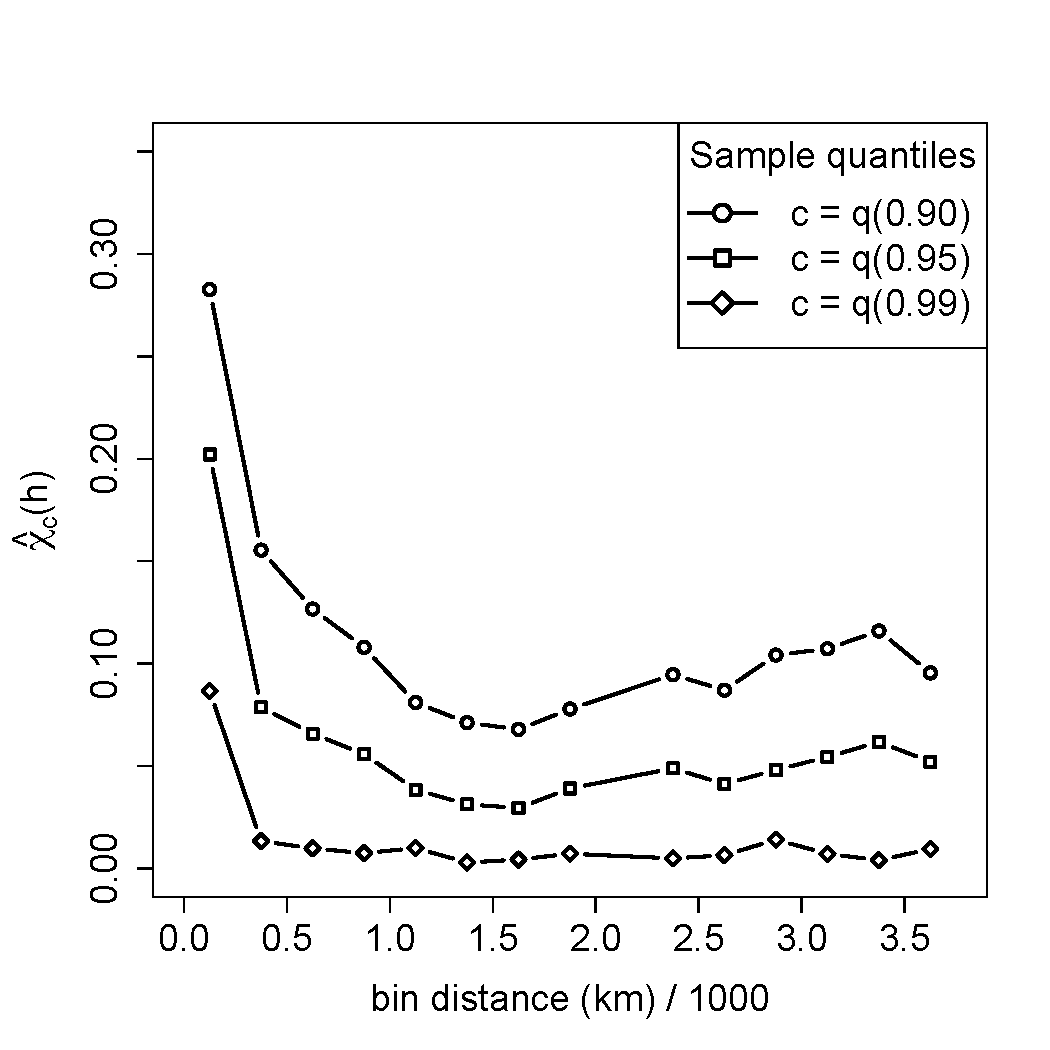
\includegraphics[width=0.49\linewidth]{plots/chi-h-ozone.pdf}
%   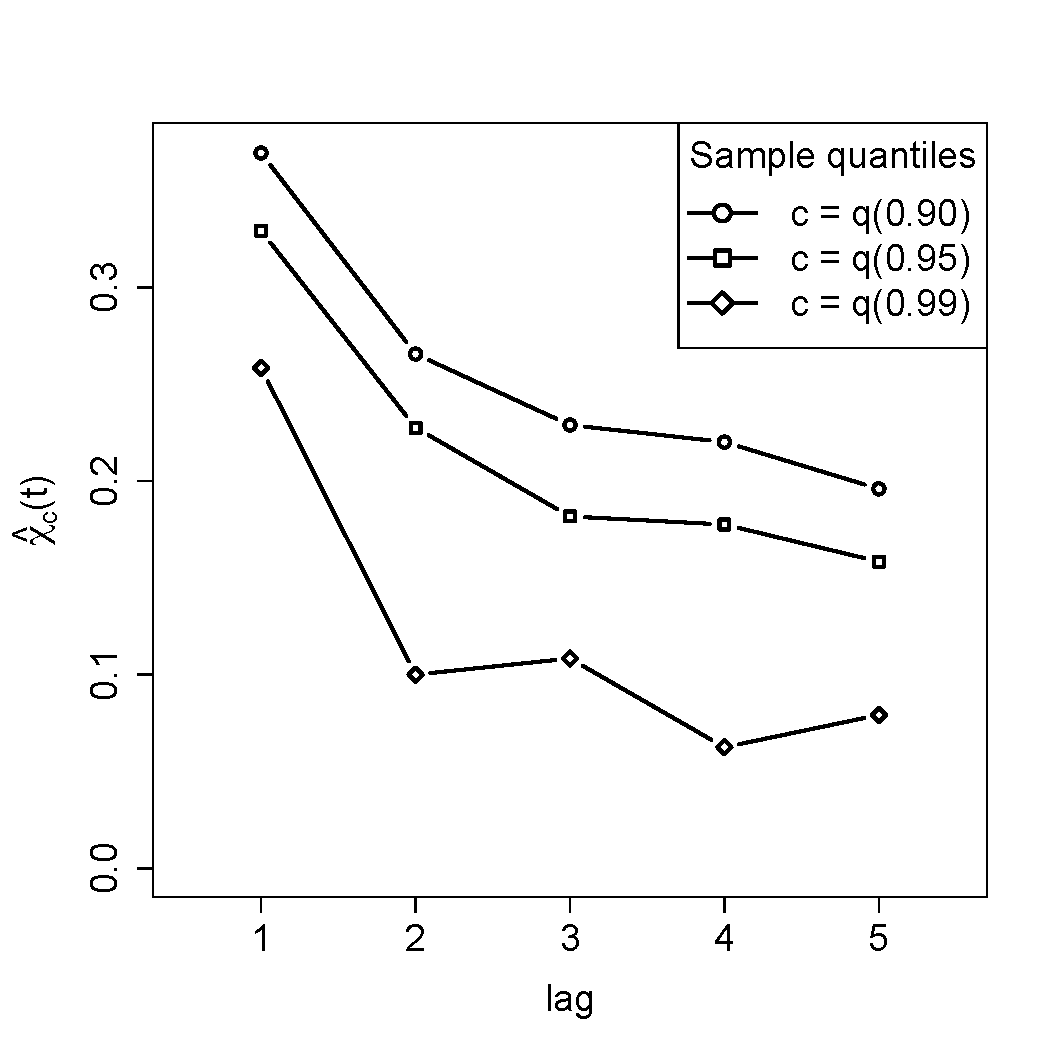
\includegraphics[width=0.49\linewidth]{plots/chi-t-ozone.pdf}
%   \caption{$\widehat{\chi}_c(h)$ plot for the residuals (left). $\widehat{\chi}_c(t)$ plot for the residuals (right).}
%   \label{stfig:chi-st}
% \end{figure}

\subsection{Model comparisons}
We fit the model using Gaussian and \skewt marginal distributions with $K=1, 5, 6, 7, 8, 9, 10, 15$ partitions.
We censored $Y(\bs)$ at $T = 0$, $T = 50$ (0.42 sample quantile), and $T = 75$ (0.92 sample quantile) ppb in order to compare results from no, moderate, and high censoring.
The upper threshold of 75 ppb was used because the current air quality standard is based on exceedance of 75 ppb.
As with the simulation study, for models with a threshold of $T = 75$, we used a symmetric-$t$ marginal distribution.
We also compared models with no time series to models that included the time series.
Finally, as a comparison to max-stable methods, we fit the model using the hierarchical max-stable model of \citet{Reich2012} with the data thresholded at $T = 75$.
All methods assumed $\bX_t(\bs) = [1, \text{CMAQ}_t(\bs)]^\top$.
To ensure that the max-stable method ran in a reasonable amount of time, we used a stratified sub-sample of 800 sites.
We conducted two-fold cross validation using 400 training sites and 400 validation sites as described in \sref{sts:modelselect}

Each chain of the MCMC ran for 30,000 iterations with a burn-in period of 25,000 iterations.
We used the same priors for the spatial covariance parameters, skewness parameter, and knots as in the simulation study.
The prior for the residual variance terms was $\sigma^2_t(\bs) \sim \text{IG}(a / 2, b / 2)$ where $a$ was the same as the simulation study, but $b$ had a Gamma$(1, 1)$ prior.
Parameters appeared to converge properly; however, as before, for models with multiple partitions it was hard to assess the convergence of $\bw$, $z(\bs)$, and $\sigma^2(\bs)$ because of partition label switching throughout the MCMC.
For each model, we averaged Brier scores over all sites and days to obtain a single Brier score for each dataset.
At a particular level, the model that fit the best was the one with the lowest score.
We then computed the relative (to Gaussian) Brier scores (see \sref{sts:simresults}) to compare each model.

\subsection{Results}\label{sts:results}
The results suggest that the \skewt, thresholded, partitioned, and time series models all give an improvement in predictions over the Gaussian model, whereas the max-stable method results in relative Brier scores between 1.13 and 1.18 indicating poorer performance than the Gaussian model.
The plots in \fref{stfig:bs-ozone} show the relative Brier scores for time-series and non-time-series models, using $K = $ 1, 7, and 15 knots at thresholds $T = $ 0, 50, and 75 ppb.
Most of the models perform similarly across all the Brier scores; however, for single-partition models without thresholding, performance tends to diminish in the extreme quantiles.
The results also suggest that thresholding improves performance for estimates in the extreme quantiles.
Both plots have similar features suggesting that most settings do reasonably well.
In particular, for all extreme quantiles, selecting a moderate number of knots (e.g. $K = 5, \ldots, 10$) tends to give the best results.
\tref{sttbl:ozoneresults} shows the best two models for selected extreme quantiles.

We illustrate the predictive capability of our model in \fref{stfig:ozoneq99} by plotting the 99th quantile for South Carolina and Georgia, a subset of the spatial domain, in order to study local features.
The four methods used are
\begin{enumerate}
  \item Gaussian
  \item \Skewt, $K =$ 1 knot, $T = $ 0, no time series
  \item \Skewt, $K =$ 5 knots, $T = $ 50, no time series
  \item Symmetric-$t$, $K =$ 10 knots, $T = $ 75, time series.
\end{enumerate}
In the bottom two plots, we plot the differences between method 4 and methods 1 and 2.
The most noticeable differences between the reference methods and the comparison methods is that the comparison methods tend to give higher estimates of the 99th quantile along the I-85 corridor between Charlotte and Atlanta.
Among these methods, the fourth method demonstrates the best performance.
For a map of Brier scores for the 99th quantile between Gaussian and the fourth method, see \aref{sta:ozonesite}.

\begin{figure}
  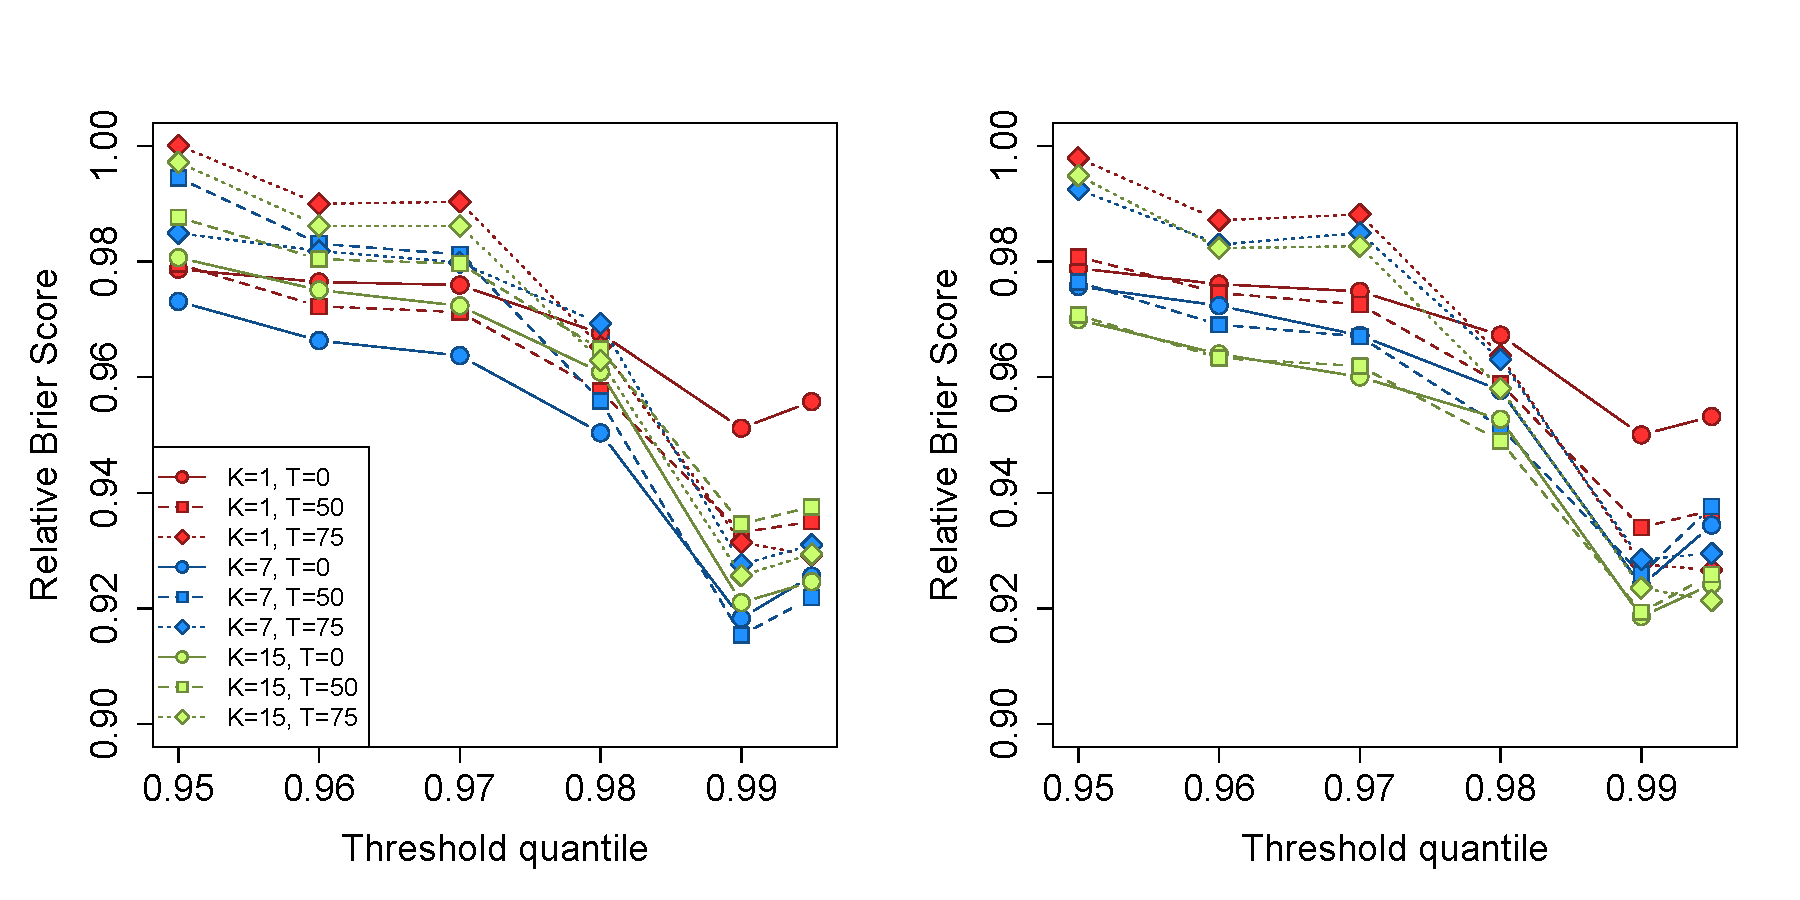
\includegraphics[width=\linewidth]{plots/bs-ozone.pdf}
  \caption{Relative Brier scores for time-series models (left) and non-time-series models (right). Relative brier score for the max-stable model is between 1.13 and 1.18}
  \label{stfig:bs-ozone}
\end{figure}
\begin{table}
  \scriptsize
  \caption{Top two performing models for predicting ozone exceedance of level $L$ with Relative Brier score}
  \label{sttbl:ozoneresults}
  \centering
  \begin{tabular}{l c l l l c c l l l c}
    \toprule
     \multicolumn{1}{c}{$L$} &\phantom{ab} & \multicolumn{4}{c}{1st} & \phantom{a} & \multicolumn{4}{c}{2nd} \\
    \cmidrule{1-1} \cmidrule{3-6} \cmidrule{8-11}
    $q(0.90)$  && No time series & $K=6$  & $T=50$  & BS: 0.992 &&
                 No time series & $K=1$  & $T=0$  & BS: 0.992 \\
    $q(0.95)$  && Time series & $K=5$ & $T=50$ & BS: 0.988 &&
                 No time series & $K=6$  & $T=50$ & BS: 0.989\\
    $q(0.98)$  && Time series & $K=7$  & $T=50$ & BS: 0.973 &&
                 Time series & $K=5$ & $T=50$ & BS: 0.975\\
    $q(0.99)$  && No time series    & $K=8$ & $T=0$ & BS: 0.946 &&
                 Time series    & $K=9$  & $T=75$ & BS: 0.947\\
    $q(0.995)$ && No time series    & $K=8$  & $T=0$ & BS: 0.951 &&
                 Time series    & $K=9$ & $T=75$ & BS: 0.956\\
    \bottomrule
  \end{tabular}
\end{table}

\begin{figure}
  \centering
  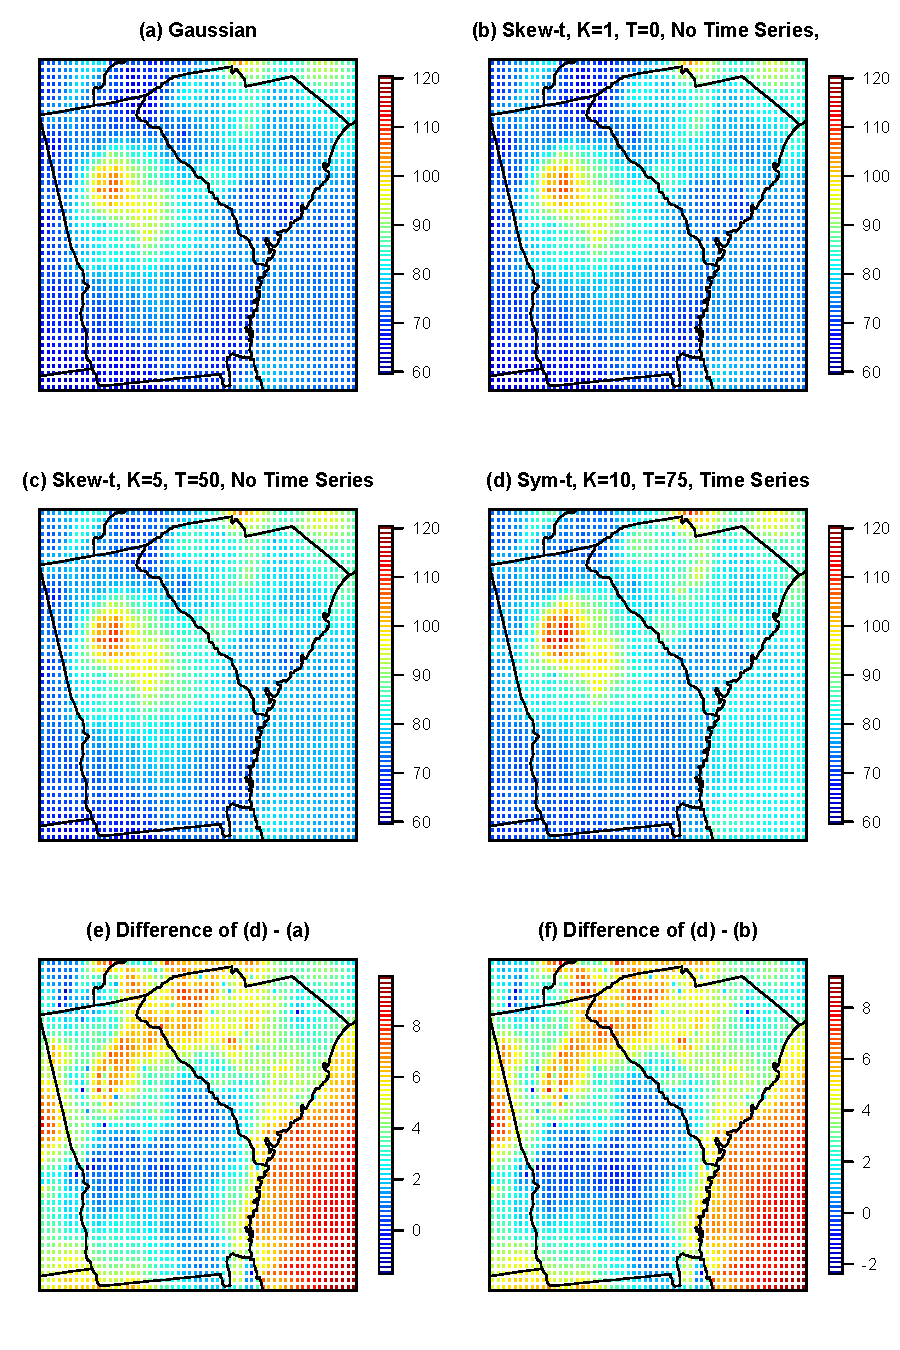
\includegraphics[height=0.95\textheight]{plots/q99-ozone.pdf}
  \caption{Panels (a) -- (d) give the posterior predictive $\widehat{q}(0.99)$ for the month of July under four different models, panel (e) gives the difference between $\widehat{q}(0.99)$ in panels (d) and (a), panel (f) gives the difference between $\widehat{q}(0.99)$ in panels (d) and (b).}
  \label{stfig:ozoneq99}
\end{figure}

\section{Discussion}\label{sts:con}
In this paper we propose a new threshold exceedance approach for spatiotemporal modeling based on the \skewt process.
The proposed model gives flexible tail behavior, demonstrates asymptotic dependence for observations at sites that are near to one another, and has computation on the order of Gaussian models for large space-time datasets.
In the simulation study, we demonstrate that this model shows statistically significant improvements over a na\"{i}ve Gaussian approach and in most cases, a max-stable approach.
In both the simulation study, and the application to ozone data, we find that incorporating a partition in the model can improve extreme predictions.
Furthermore the results from the data analysis suggest that thresholding can improve performance when predicting in the extreme tails of the data.

This model presents new avenues for future research.
One possibility is the implementation of a different partition structure.
We choose to define the random effects for a site by using an indicator function based on closeness to a knot.
However, this indicator function could be replaced by kernel function that would allow for multiple knots to impact each site, with the weight of each knot to be determined by some characteristic such as distance.
Another area that should be explored is the temporal dependence in the model.
Instead of implementing a time series on the random effects, a three-dimensional covariance structure on the residuals could be implemented to address temporal dependence.
Finally, we acknowledge that by specifying the number of knots, we may be underestimating the uncertainty in the model.
This could be incorporated by treating the number of knots as a model parameter instead of fixing it to be a specific value.

\graphicspath{{./Chapter-3/}}
\chapter{A Spatial Model for Rare Binary Events}
\chaptermark{Spatial Rare Binary}
\label{chap:three}

\section{Introduction}\label{rbs:intro}

The goals of spatial binary data analysis are often to estimate covariate effects while accounting for spatial dependence and to make predictions at locations without samples.
A common approach to incorporate spatial dependence in the model for binary data is relating a continuous spatial process $Z(\bs) \in \mathbb{R}$ to the binary response $Y(\bs)$ by thresholding, $Y(\bs) = I[Z(\bs) > c]$, where $I[\cdot]$ is an indicator function.
In many spatial analyses of binary data, a Gaussian process is used to model $Z(\bs)$.
This is true for both spatial probit and spatial logistic regression.
In these models, spatial dependence is determined by the joint probability that two sites simultaneously exceed the threshold $c$.
However, when $c$ is large, and thus $Y(\bs) = 1$ is rare, then the asymptotic theory suggests that the Gaussian process will model dependence poorly.
In fact, even under strong spatial correlation for $Z(\bs)$, it gives asymptotic independence \citep{Sibuya1960}, suggesting that for rare binary data, the Gaussian model will not perform very well.

We propose using a latent max-stable process \citep{deHaan1984} for $Z(\bs)$ because it allows for asymptotic dependence.
The max-stable process arises as the limit of the location-wise maximum of infinitely many spatial processes, and any finite-dimensional representation of a max-stable process has generalized extreme value distribution (GEV) marginal distributions.
Max-stable processes are extremely flexible, but are often challenging to work with in high dimensions \citep{Wadsworth2014,Thibaud2013a}.
To address this challenge, methods have been proposed that implement composite likelihood techniques for max-stable processes \citep{Padoan2010,Genton2011,Huser2014}.
Composite likelihoods have also been used to model binary spatial data \citep{Heagerty1998}, but not using max-stable processes.
As an alternative to these composite approaches, \citet{Reich2012} present a hierarchical model that implements a low-rank representation for a max-stable process.
We choose to use this low-rank representation for our rare binary spatial regression model.
Our model builds on related work by \citet{Wang2010} who use a GEV link for non-spatial binary data.
The proposed model generalizes this to have spatial dependence.

The paper proceeds as follows.
In \sref{rbs:maxstab} we present the proposed latent max-stable process for spatially dependent rare binary analysis.
In \sref{rbs:multivariate} we give the bivariate distribution for our model.
In \sref{rbs:spatdep} we show a link between a commonly used measure of dependence between binary variables and another metric for extremal dependence.
The computing for our model is outlined in \sref{rbs:comp}.
Finally, we present a simulation study in \sref{rbs:sim} which is followed in \sref{rbs:dataanalysis} by a data analysis of two species: \tamarix{} and \hedysarum{}.
Lastly, in \sref{rbs:conclusions} we provide some discussion and possibilities for future research.

\section{Spatial dependence for binary regression} \label{rbs:maxstab}

Let $Y(\bs)$ be the binary response at spatial location $\bs$ in a spatial domain of interest $\calD \in \mathbb{R}^2$.
We assume $Y(\bs) = I[Z(\bs) > 0]$ where $Z(\bs)$ is a latent continuous max-stable process.
The marginal distribution of $Z(\bs)$ at site $\bs$ is GEV with location $\bX(\bs)^\top \bbeta$, scale $\sigma > 0$, and shape $\xi$, where $\bX(\bs)$ is a $p$-vector of spatial covariates at site $\bs$ and $\bbeta$ is a $p$-vector of regression coefficients.
We set $\sigma = 1$ for identifiability because only the sign and not the scale of $Z$ affects $Y$.
If $\bX(\bs)^\top \bbeta = \mu$ for all $\bs$, then $P(Y = 1)$ is the same for all observations, and the two parameters $\mu$ and $\xi$ are not individually identifiable.
So when there are no covariates, we fix $\xi = 0$.
Although $\bbeta$ and $\xi$ could be permitted to vary across space, we assume that they are constant across $\calD$.
At spatial location $\bs$, the marginal distribution (over $Z(\bs)$) is
\begin{align}
	P[Y(\bs) = 1] = 1 - \exp\left\{ -\displaystyle\frac{ 1 }{ z(\bs)} \right\}
\end{align}
where $z(\bs) = \left[1 - \xi \bX(\bs)^\top \bbeta\right]^{1 / \xi}$.
This is the same as the marginal distribution given by \citet{Wang2010}.

For a finite collection of locations $\bs_1, \ldots, \bs_n,$ we denote by $\bY = [Y(\bs_1), \ldots, Y(\bs_n)]^\top$ the vector of observations.
The spatial dependence of $\bY$ is determined by the joint distribution of the latent variable $\bZ = [Z(\bs_1),\ldots, Z(\bs_n)]^\top$.
To incorporate spatial dependence, we consider the hierarchical representation of the max-stable process proposed in \citet{Reich2012}.
Consider a set of positive stable (PS) random effects $A_1, \ldots, A_L \iid \text{PS}(\alpha)$ associated with spatial knots $\bv_1, \ldots, \bv_L \in \mathbb{R}^2$.
The hierarchical model is given by
\begin{align} \label{rbeq:hiermodel}
Z(\bs_i) | A_1, \ldots, A_L \ind \text{GEV}\left[\bX(\bs_i)^\top \bbeta + \frac{\theta(\bs_i)^\xi - 1}{\xi}, \alpha \theta(\bs_i), \xi \alpha\right] \quad \text{and} \quad \theta(\bs_i) = \left[\sum_{l = 1}^L A_l w_l (\bs_i)^{1 / \alpha} \right]^\alpha
\end{align}
where $w_{l}(\bs_i) > 0$ are a set of $L$ weight functions that vary smoothly across space and satisfy the condition \mbox{$\displaystyle \sum_{l = 1}^L w_l(\bs) = 1$} for all $\bs$, and $\alpha\in(0,1)$ determines the strength of dependence, with $\alpha$ near zero giving strong dependence and $\alpha=1$ giving joint independence.

Because the latent $\bZ(\bs)$ are independent given the random effects $\theta(\bs)$, the binary responses are also conditionally independent.
This leads to the tractable likelihood
\begin{align} \label{rbeq:condlike}
Y(\bs_i) | A_l, \ldots, A_L &\ind \text{Bern}[\pi(\bs_i)]
\end{align}
where
\begin{align} \label{rbeq:pyeq1cond}
\pi(\bs_i) &= 1 - \exp \left\{ -\displaystyle \sum_{ l = 1 }^{L} A_l \left[ \frac{ w_{l}(\bs_i) }{ z(\bs_i) } \right]^{ 1/\alpha} \right\}
\end{align}
and $z(\bs) = [1 + \xi \bX(\bs)^\top \bbeta)]^{1 / \xi}$.
Marginally over the $A_l$, this gives
\begin{align}
Z(\bs) \sim \text{GEV}\left[\bX(\bs)^\top \bbeta, 1, \xi\right],
\end{align}
and thus $P[Y(\bs) = 1] = 1 - \exp\left\{-\displaystyle \frac{1}{z(\bs)}\right\}$.

Many weight functions are possible, but the weights must be constrained so that $\displaystyle \sum_{l=1}^L w_{l}(\bs_i)=1$ for $i=1,\ldots,n$ to preserve the marginal GEV distribution.
For example, \cite{Reich2012} take the weights to be scaled Gaussian kernels with knots $\bv_l$,
\begin{align}\label{rbeq:w}
w_{l}(\bs_i) = \frac{\exp\left[-0.5\left(||\bs_i-\bv_l||/\rho\right)^2\right]}
{\displaystyle \sum_{j=1}^L\exp\left[-0.5\left(||\bs_i-\bv_j||/\rho\right)^2\right]}
\end{align}
where $||\bs_i - \bv_l||$ is the distance between site $\bs_i$ and knot $\bv_l$, and the kernel bandwidth $\rho>0$ determines the spatial range of the dependence, with large $\rho$ giving long-range dependence and vice versa.

After marginalizing out the positive stable random effects, the joint distribution of $\bZ$ is
\begin{align}\label{rbeq:jointCDF}
G(\bz) = P\left[Z(\bs_1) < z(\bs_1), \ldots, Z(\bs_n) < z(\bs_n)\right] = \exp\left\{-\sum_{l=1}^L\left[\sum_{i=1}^n\left(\frac{w_{l}(\bs_i)}{z(\bs_i)}\right)^{1/\alpha}\right]^{\alpha}\right\},
\end{align}
where $G(\cdot)$ is the CDF of a multivariate GEV distribution.
This is a special case of the multivariate GEV distribution with asymmetric Laplace dependence function \citep{Tawn1990}.

\section{Joint distribution}\label{rbs:multivariate}

We give an exact expression in the case where there are only two spatial locations which is useful for constructing a pairwise composite likelihood \citep{Padoan2010} and studying spatial dependence.
When $n = 2$, the probability mass function is given by
\begin{align} \label{rbeq:biv}
\text{P}[Y(\bs_i) = y_i, Y(\bs_j) = y_j] = \begin{cases}
\varphi(\bz), &y_i = 0, y_j = 0\\
\exp\left\{ - \displaystyle \frac{ 1 }{ z(\bs_i) } \right\} - \varphi(\bz), &y_i = 1, y_j = 0 \\
\exp\left\{ - \displaystyle \frac{ 1 }{ z(\bs_j) } \right\} - \varphi(\bz), &y_i = 0, y_j = 1 \\
1 - \exp\left\{ - \displaystyle\frac{ 1 }{ z(\bs_i) } \right\} - \exp \left\{ -\displaystyle \frac{ 1 }{z(\bs_j)} \right\} + \varphi(\bz), \quad &y_i = 1, y_j = 1
\end{cases}
\end{align}
where $\varphi(\bz) = \exp \left\{ - \displaystyle \sum_{ l = 1 }^{ L } \left[ \left( \displaystyle \frac{ w_{ l }(\bs_i) }{ z(\bs_i) } \right)^{1/\alpha} + \left( \displaystyle \frac{ w_{l }(\bs_j)}{z(\bs_j)} \right)^{1/\alpha} \right]^{\alpha} \right\}$.
For more than two locations, we are also able to compute the exact likelihood when $n$ is large but the number of events $K = \displaystyle \sum_{i = 1}^n Y(\bs_i)$ is small, as might be expected for very rare events, see \aref{rba:likelihoodderivation}.

% - Assume Z1 and Z2 are both GEV(\beta,1,1) so that the probability of Yi=1 decreases to zero as beta increases
% - A common measure of dependence between binary variables is Cohen’s Kappa, K(beta) =
% - For the spatial model we get K(beta)=
% - To measure extremal dependence let beta go to infinity so that event are increasing more rare
% - K = limK(beta) = …
% - This is similar to the extremal coefficient in Reich and Shaby

\section{Quantifying spatial dependence} \label{rbs:spatdep}

Assume that $Z(\bs_1)$ and $Z(\bs_2)$ are both GEV$(\beta, 1, 1)$ so that $P(Y_i = 1)$ decreases to zero as $\beta$ increases.
A common measure of dependence between binary variables is Cohen's kappa \citep{Cohen1960},
\begin{align}
\kappa(\beta) = \frac{P_A - P_E}{1 - P_E}
\end{align}
where $P_A$ is the joint probability of agreement $P(Y_1 = Y_2)$ and $P_E$ is the joint probability of agreement under an assumption of independence $P(Y_i = 1)^2 + P(Y_i = 0)^2$.
For the spatial model,
\begin{align*}
P_A(\beta) &= 1 - 2 \exp\left\{ -\frac{1}{\beta} \right\} + 2 \exp\left\{-\frac{\vartheta(\bs_1, \bs_2)}{\beta}  \right\} \nonumber \\
P_E(\beta) &= 1 - 2 \exp \left\{ -\frac{1}{\beta} \right\} + 2 \exp \left\{ -\frac{2}{\beta} \right\}, \nonumber
\end{align*}
and
\begin{align} \label{rbeq:kappa}
\kappa(\beta) &= \frac{P_A(\beta) - P_E(\beta)}{1 - P_E(\beta)} = \frac{\exp\left\{-\displaystyle\frac{\vartheta(\bs_1, \bs_2) - 1}{\beta}  \right\} - \exp \left\{ -\displaystyle\frac{1}{\beta} \right\}}{1 - \exp \left\{ -\displaystyle\frac{1}{\beta} \right\}}
\end{align}
where $\vartheta (\bs_i, \bs_j) = \displaystyle \sum_{ l = 1 }^{ L } \left[ w_{l}(\bs_i)^{ 1/\alpha } +  w_{ l}(\bs_j)^{ 1/\alpha } \right]^\alpha$ is the pairwise extremal coefficient given by \citet{Reich2012}.
To measure extremal dependence, let $\beta \rightarrow \infty$ so that events are increasingly rare.
Then,
\begin{align}
\kappa = \lim_{\beta \rightarrow \infty} \kappa(\beta) = 2 - \vartheta(\bs_1, \bs_2)
\end{align}
which is the same as the $\chi$ statistic of \citet{Coles2001}, a commonly used measure of extremal dependence.

\section{Computation}\label{rbs:comp}

For small $K$, we can evaluate the likelihood directly.
When $K$ is large, we use Markov chain Monte Carlo (MCMC) methods with the random effects model to explore the posterior distribution.
To overcome challenges with evaluating the positive stable density, we follow \citet{Reich2012} and introduce a set of auxiliary variables $B_1, \ldots, B_L$ following the auxiliary variable technique of \citet{Stephenson2009} \citep[see Appendix A.3]{Reich2012}.
So, the hierarchical model is given by
\begin{align}
Y(\bs_i) | \pi(\bs_i) &\ind \text{Bern}[\pi(\bs_i)] \\
\pi(\bs_i) &= 1 - \exp \left\{ -\displaystyle \sum_{ l = 1 }^{L} A_l \left[ \frac{ w_{l}(\bs_i) }{ z(\bs_i) } \right]^{ 1/\alpha} \right\} \nonumber\\
% Z(\bs_i) | A_l, \ldots, A_L &\ind \text{GEV}[\bX(\bs_i)^\top \bbeta + \theta(\bs_i), \alpha \theta(\bs_i), \xi \alpha] \nonumber\\
A_l &\sim \text{PS}(\alpha) \nonumber
\end{align}
with priors $\bbeta \sim \text{N}(\bZero, \sigma^2_\beta \bI_p )$, $\xi \sim \text{N}(0, \sigma^2_\xi)$, $\rho \sim \text{Unif}(\rho_l, \rho_u)$, and $\alpha \sim \text{Beta}(a_\alpha, b_\alpha)$.
The model parameters are updated using Metropolis Hastings (MH) update steps, and the random effects $A_1, \ldots, A_L$, and auxiliary variables $B_1, \ldots, B_L$ are updated using Hamiltonian Monte Carlo (HMC) update steps.
The code for this is available online through \url{https://github.com/sammorris81/rare-binary}.

\section{Simulation study}\label{rbs:sim}

For our simulation study, we generate $n_m = 50$ datasets under 12 different simulation settings to explore the impact of sample size, sampling technique, and misspecification of link function.
We generate data from three possible underlying processes.
For each of the underlying processes, we generate complete datasets on a $100 \times 100$ rectangular grid of $n = 10,000$ locations.
If a simulated population is generated and $K < 50$, it is discarded and a new simulated population is generated.
This is done to guarantee that the rarity for all datasets is no lower than $0.5\%$.
For model fitting, we select a subsample and use the remaining sites to evaluate predictive performance.
For all models, we run the MCMC sampler for 25,000 iterations with a burn-in period of 20,000 iterations.
Convergence is assessed through visual inspection of traceplots.

\subsection{Latent processes} \label{rbs:simsettings}

The first process is a latent max-stable process that uses the GEV link described in \eref{rbeq:hiermodel} with knots on a $50 \times 50$ regularly spaced grid on $[0, 1] \times [0, 1]$.
For this process, we set $\alpha = 0.35$, $\rho = 0.1$, and $\beta_0 \approx 2.97$ which gives $K = 500$ (5\% rarity), on average.
Because there are no covariates, we set $\xi = 0$.
We then set $Y(\bs) = I[Z(\bs) > 0]$.

For the second process, we generate a latent variable from a spatial Gaussian process with a mean of $\text{logit}(0.05) \approx -2.94$ and an exponential covariance given by
\begin{align}
\text{Cov}(\bs_1, \bs_2) = \tau_\text{Gau}^2 \exp\left\{- \frac{||\bs_1 - \bs_2||}{\rho_\text{Gau}}\right\}
\end{align}
with $\tau_\text{Gau} = 10$ and $\rho_\text{Gau} = 0.1$.
Finally, we generate $Y(\bs_i) \ind \text{Bern}[\pi(\bs_i)]$
where $\pi(\bs_i) = \displaystyle \frac{ \exp\{z(\bs)\}}{1 + \exp\{z(\bs)\} }$.

For the third process, we generate data using a hotspot method.
For this process, we first generate hotspots throughout the space.
Let $n_\text{hs}$ be the number of hotspots in the space.
Then \mbox{$n_\text{hs} - 1 \sim$ Poisson$(2)$}.
This generation scheme ensures that every dataset has at least one hotspot.
We generate the hotspot locations $\bh_1, \ldots, \bh_{n_\text{hs}} \sim$ Unif$(0, 1)^2$.
Let $B_h$ be a circle of radius of radius $r_h$ around hotspot $h = 1, \ldots, n_\text{hs}$.
The $r_h$ differ for each hotspot and are generated i.i.d. from a Unif$(0.03, 0.08)$ distribution.
We set $P[Y(\bs_i) = 1] = 0.85$ for all $\bs_i$ in $B_h$, and $P[Y(\bs_i) = 1] = 0.0005$ for all $\bs_i$ outside of $B_h$.
These settings are selected to give an average of approximately $K = 500$ for the datasets.
\fref{rbfig:simulateddata} gives an example dataset from each of the data settings.

\begin{figure}  % code/analysis/simstudy/combine-tables.R
	\centering
	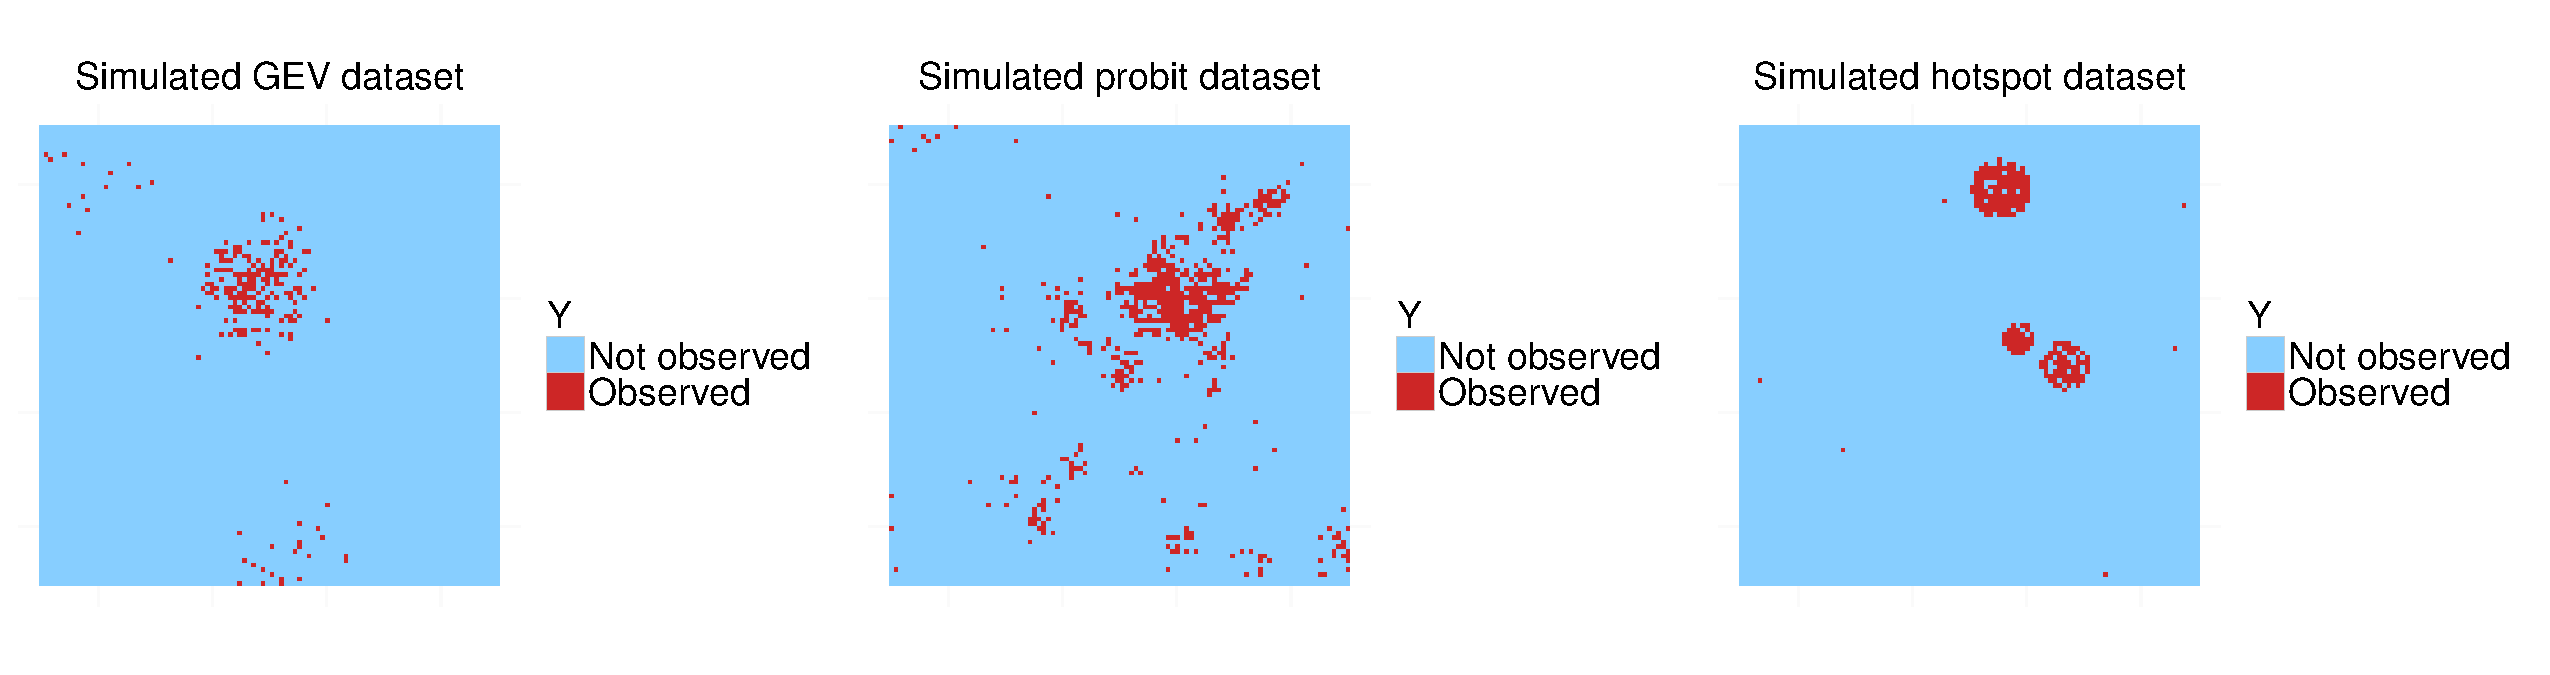
\includegraphics[width=\linewidth, trim={0em, 1em, 0em, 1em}]{plots/simulateddata}
	\caption{One simulated dataset from spatial GEV (left), spatial logistic (center), and hotspot (right) designs.}
	\label{rbfig:simulateddata}
\end{figure}

\subsection{Sampling methods} \label{rbs:simsampling}

We subsample the generated data using $n_s = 100$, $250$ initial locations for two different sampling designs.
The first is a two-stage spatially-adaptive cluster technique (CLU) taken from \citet{Pacifici2016}.
In this design, if an initial location is occupied, we also include the four rook neighbor (north, east, south, and west) sites in the sample.
For the second design, we use a simple random sample (SRS) with the same number of sites included in the cluster sample.
For the GEV setting, when $n_s = 100$, there are on average $117$ sites and at most $142$ sites in a sample, and when $n_s = 250$, there are on average $286$ sites and at most $332$ sites in a sample.
For the logistic setting, when $n_s = 100$, there are on average $118$ sites and at most $147$ sites in a sample, and when $n_s = 250$, there are on average $290$ sites and at most $330$ sites in a sample.
For the hotspot setting, when $n_s = 100$, there are on average $110$ sites and at most $128$ sites in a sample, and when $n_s = 250$, there are on average $275$ sites and at most $306$ sites in a sample.

\subsection{Methods} \label{rbs:methods}

For each dataset, we fit the model using three different models: the proposed spatial GEV model, a spatial probit model, and a spatial logistic model.
Logistic and probit methods assume the underlying process is Gaussian.
In this case, we assume that $Z(\bs)$ follows a Gaussian process with mean $\bX(\bs)^\top \bbeta$ and variance $\tau^2$.
For the simulation study, we use an intercept only model.
The marginal distributions are given by
\begin{align}
P\left[Y(\bs) = 1\right] = \begin{cases}
\displaystyle \frac{\exp\left[\bX^\top(\bs) \bbeta + \bW (\bs) \bepsilon \right]}{1 + \exp\left[\bX^\top(\bs) \bbeta + \bW (\bs) \bepsilon \right]}, \qquad &\text{logistic}\\
\Phi\left[\bX^\top \bbeta (\bs) + \bW (\bs) \bepsilon \right], \qquad &\text{probit}
\end{cases}
\end{align}
where $\bepsilon \sim$ N$(\bZero, \tau^2 \bI_L)$ are Gaussian random effects at the knot locations, and $\bW(\bs)$ are a set of $L$ basis functions given to recreate the Gaussian process at all sites.
We use our own code for the spatial probit model, but we use the \texttt{spGLM} function in the \texttt{spBayes} package \citep{Finley2015} to fit the spatial logistic model.
For the probit model, we use
\begin{align}
\bW_l(\bs_i) = \frac{\exp\left[-\left(||\bs_i-\bv_l||/\rho\right)^2\right]}
{\sqrt{\displaystyle \sum_{j=1}^L\exp\left[-\left(||\bs_i-\bv_j||/\rho\right)^2\right]^2}}.
\end{align}
For the logistic model, the $\bW_l(\bs_i)$ are the default implementation from \texttt{spGLM}.

\subsection{Priors} \label{rbs:simpriors}

For all models, we only include an intercept term $\beta_0$ in the model, and the prior for the intercept is \mbox{$\beta_0 \sim$ N$(0, 10)$}.
Additionally, for all models, the prior for the bandwidth is $\rho \sim$ Unif$(0.001, 1)$.
In all methods, we place knots at all data points.
For the GEV method, the prior for the spatial dependence parameter is $\alpha \sim$ Beta$(2, 5)$.
We select this prior because it gives greater weight to $\alpha < 0.5$, which is the point at which spatial dependence becomes fairly week, but also avoids values below 0.1 which can lead to numerical problems.
We fix $\xi = 0$ because we do not include any covariates.
For both the spatial probit and logistic models, the prior on the variance term for the random effects is IG$(0.1, 0.1)$ where IG$(\cdot)$ is an Inverse Gamma distribution.

\subsection{Model comparisons}\label{rbs:cv}

For each dataset, we fit the model using the $n_s$ observations as a training set, and validate the model's predictive power at the remaining grid points.
Let $\bs^*_j$ be the $j$th site in the validation set.
From the posterior distributions of the parameters we can calculate $P[Y(\bs^*_j) = 1]$.
To obtain $\hat{P}[Y(\bs^*_j) = 1]$, we take the average of the posterior distribution for each $\bs^*_j$.
We consider a few different metrics for comparing model performance.
One score is the Brier scores \citep[BS]{Gneiting2007}.
The Brier score for predicting an occurrence at site $\bs$ is given by $\{I[Y(\bs)=1] - \hat{P}[Y(\bs)=1]\}^2$.
We average the Brier scores over all test sites, and a lower score indicates a better fit.
The Brier score equally penalizes false negatives and false positives, but in the case of rare data, this may not be the best metric due to the unbalanced nature of the data.
Therefore, we also consider the receiver operating characteristic (ROC) curve, and the area under the ROC curve (AUROC) for the different methods and settings.
The ROC curve and AUROC are obtained via the \texttt{ROCR} \citep{Sing2005} package in \texttt{R} \citep{Rmanual}.
We then average AUROC across all datasets for each method and setting to obtain a single AUROC for each combination of method and setting.

\subsection{Results} \label{rbs:simresults}

Overall, we find that the spatial probit model actually performs quite well in all cases.
\tref{rbtbl:simbsresults} gives the Brier scores and AUROC for each of the methods.
Looking at Brier scores, we see that our model is outperformed by the probit model in all cases, and by the logistic models in many settings.
For AUROC, in a few of the settings, we do demonstrate a small improvement over the probit and logistic models.
Because these results are somewhat surprising, we also considered the performance metrics by rareness of the data.
We plot the AUROC for each link function with all sampling settings in \fref{rbfig:simsmooth-gev} -- \fref{rbfig:simsmooth-hot} using a Loess smoother.
These plots give evidence to suggest that as rareness increases, the spatial GEV method has potential to outperform the spatial probit and logistic models based on AUROC.

\begin{figure}[htbp]  % code/analysis/simstudy/combine-tables.R
	\centering
	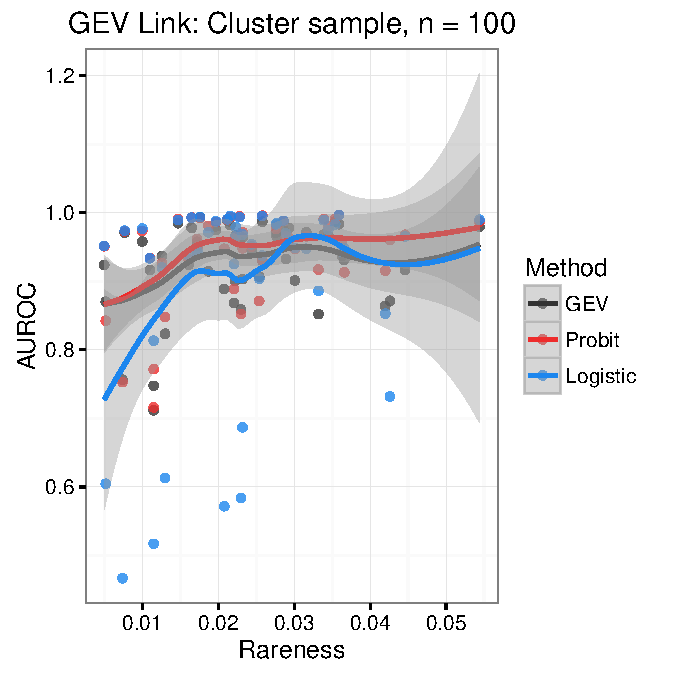
\includegraphics[width=0.47\linewidth]{plots/byrareness-1}
	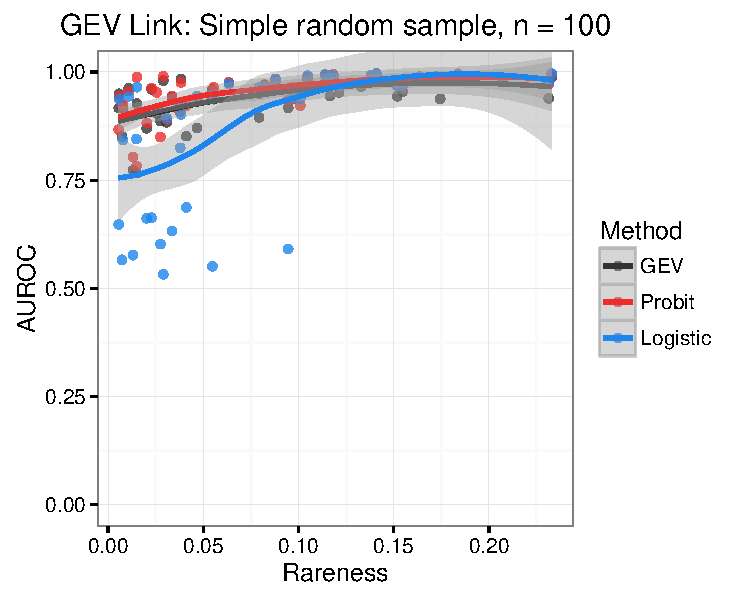
\includegraphics[width=0.47\linewidth]{plots/byrareness-2}

	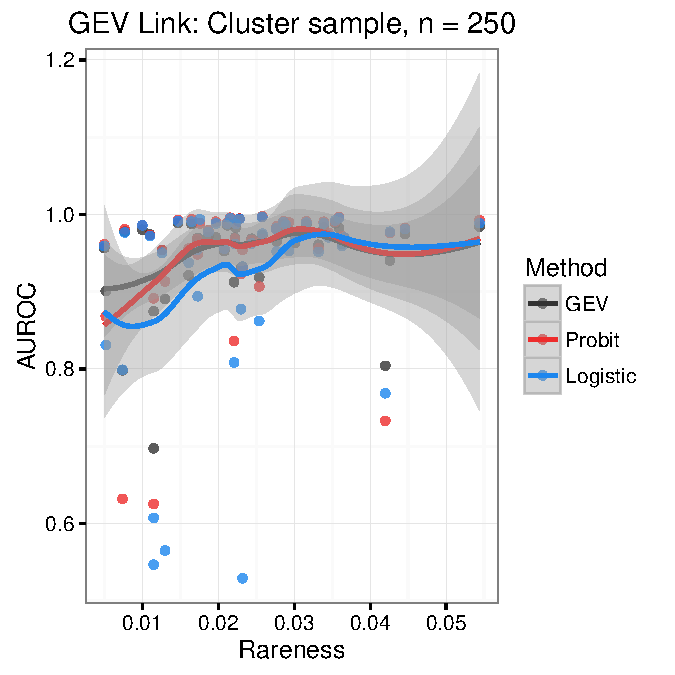
\includegraphics[width=0.47\linewidth]{plots/byrareness-3}
	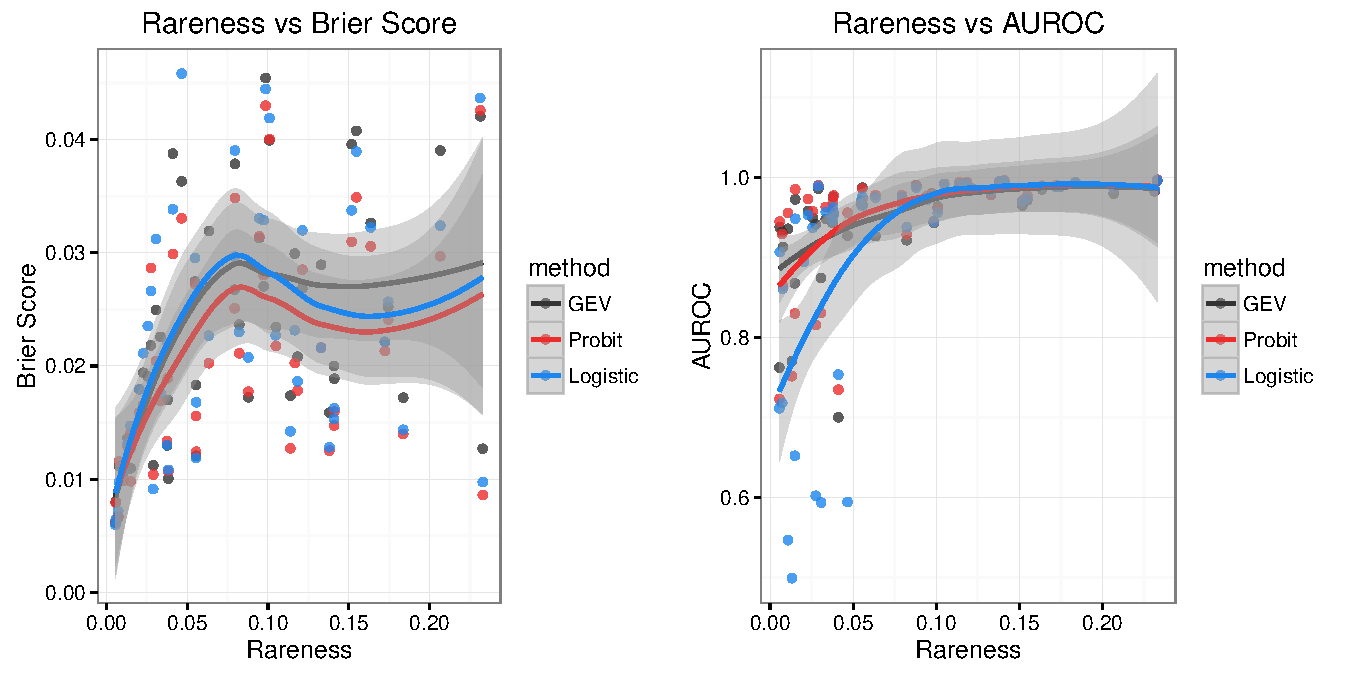
\includegraphics[width=0.47\linewidth]{plots/byrareness-4}
	\caption{Smooth of AUROC by rareness for each sample technique for the GEV link.}
	\label{rbfig:simsmooth-gev}
\end{figure}

\begin{figure}[htbp]  % code/analysis/simstudy/combine-tables.R
	\centering
	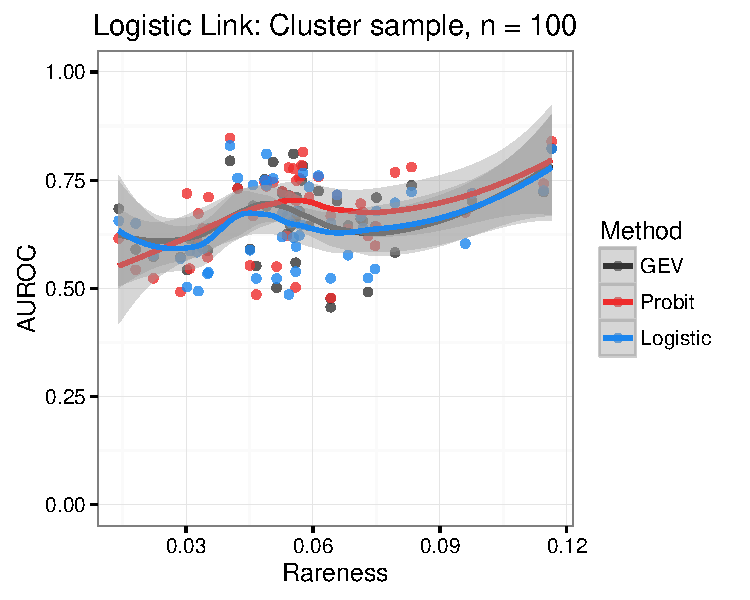
\includegraphics[width=0.47\linewidth]{plots/byrareness-5}
	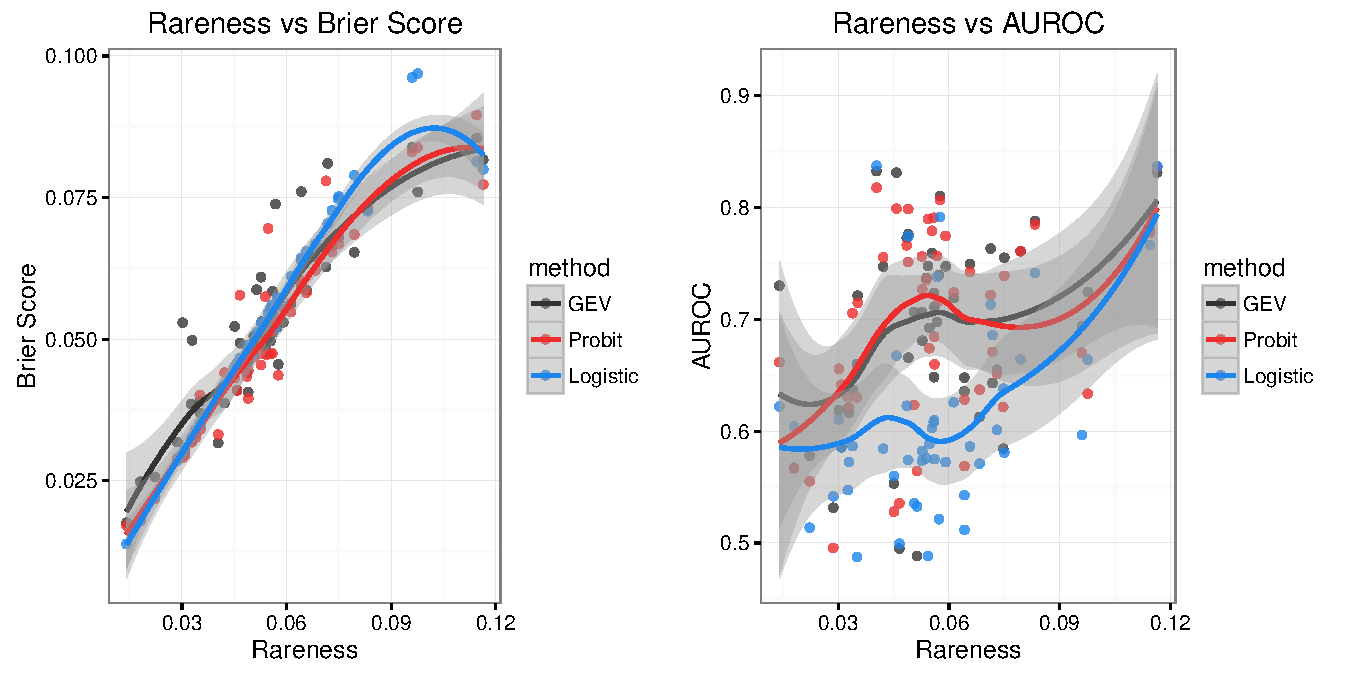
\includegraphics[width=0.47\linewidth]{plots/byrareness-6}

	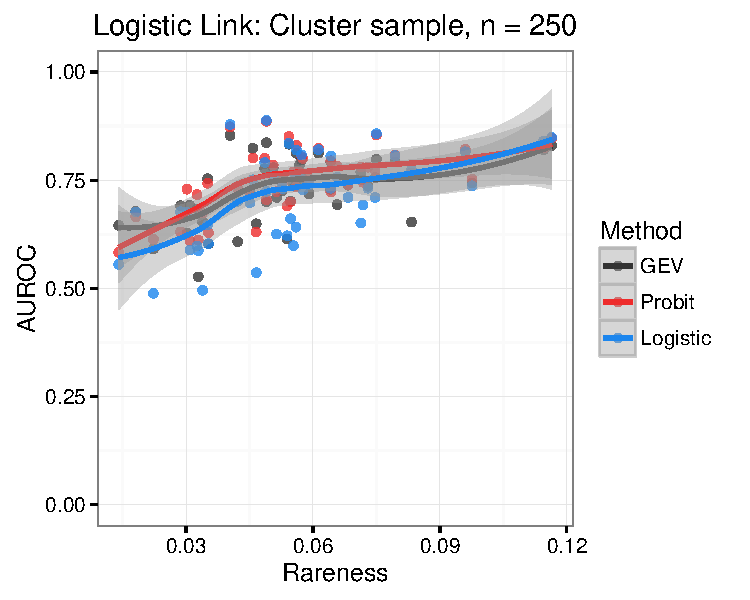
\includegraphics[width=0.47\linewidth]{plots/byrareness-7}
	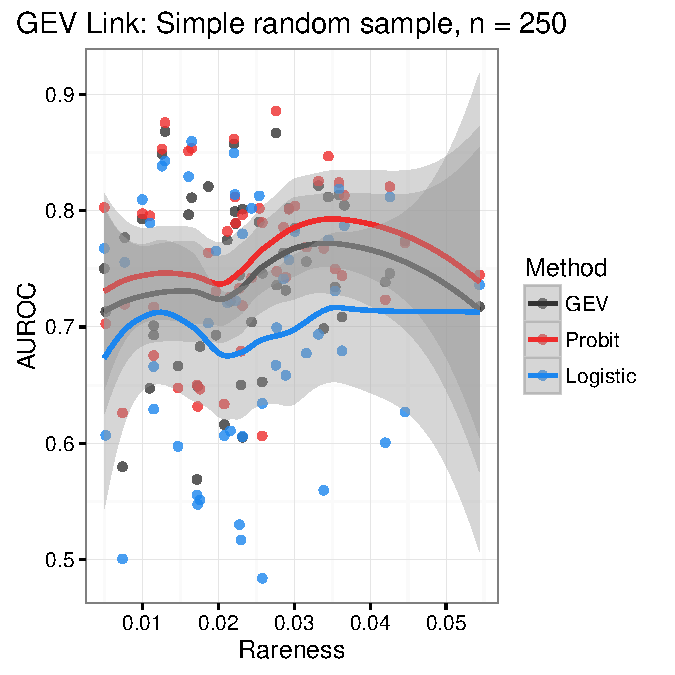
\includegraphics[width=0.47\linewidth]{plots/byrareness-8}
	\caption{Smooth of AUROC by rareness for each sample technique for the logistic link.}
	\label{rbfig:simsmooth-log}
\end{figure}

\begin{figure}[htbp]  % code/analysis/simstudy/combine-tables.R
	\centering
	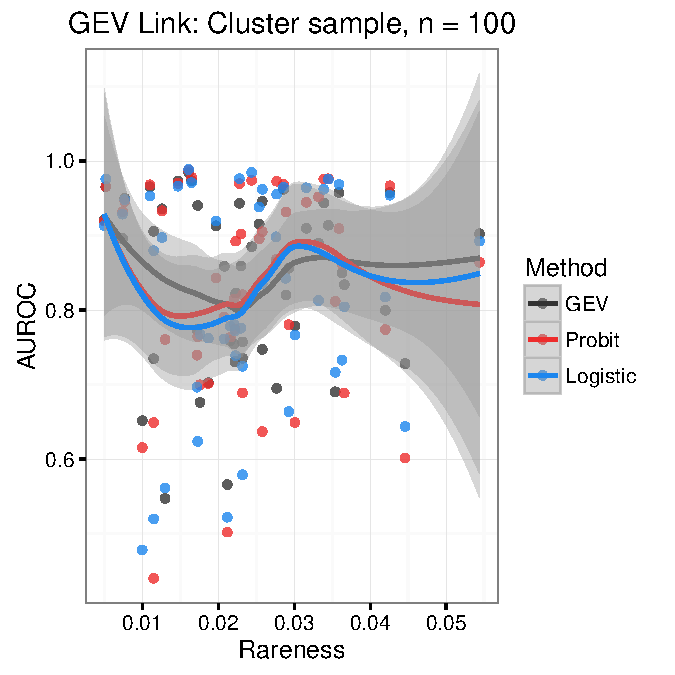
\includegraphics[width=0.47\linewidth]{plots/byrareness-9}
	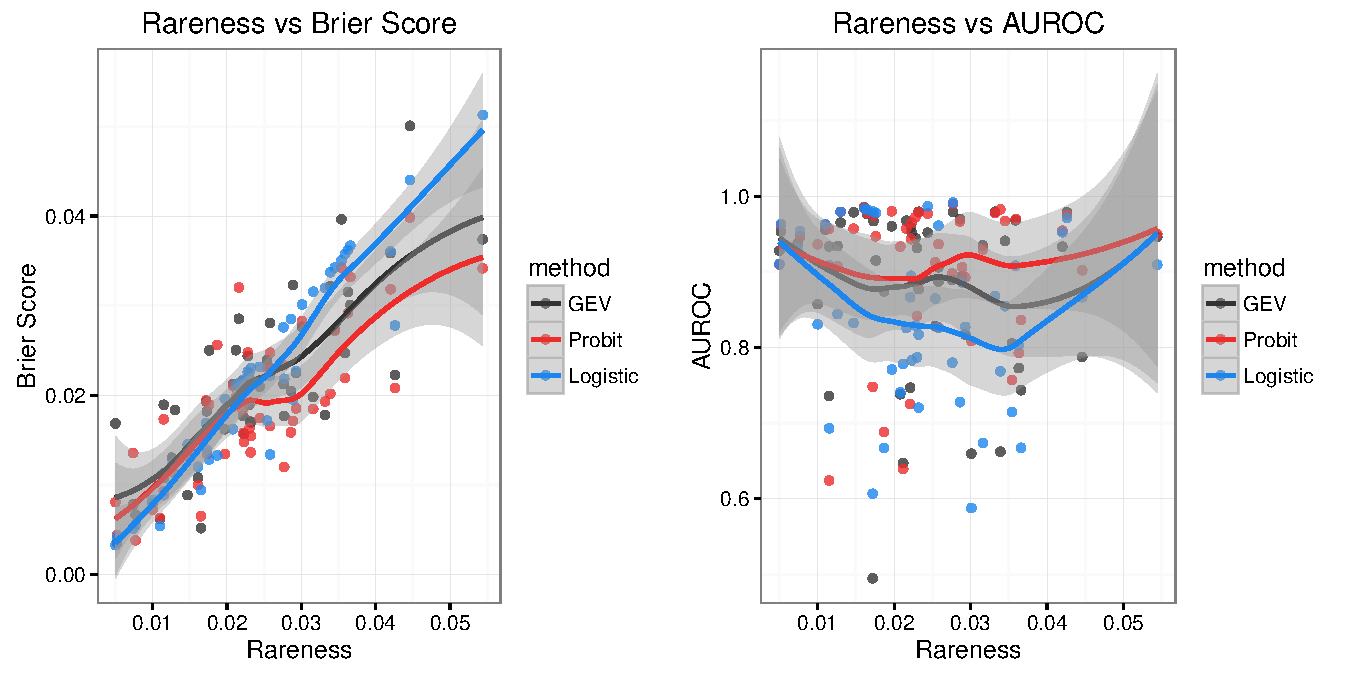
\includegraphics[width=0.47\linewidth]{plots/byrareness-10}

	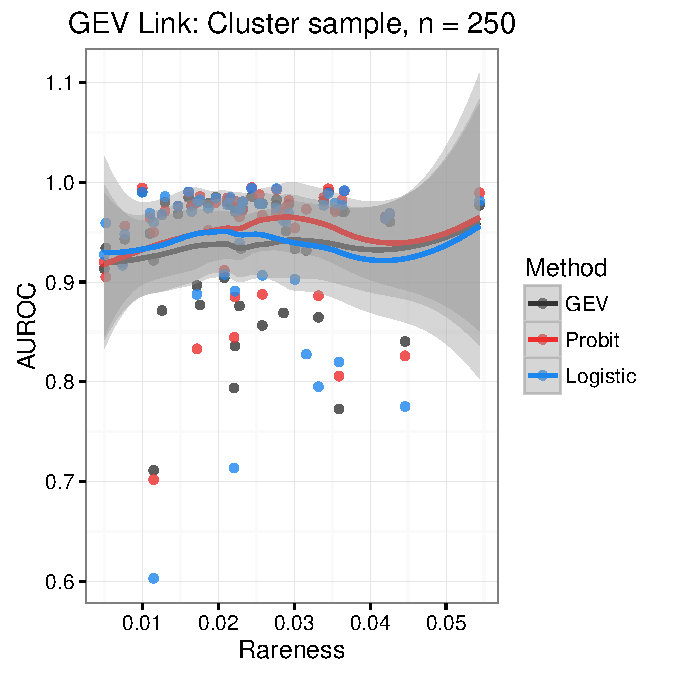
\includegraphics[width=0.47\linewidth]{plots/byrareness-11}
	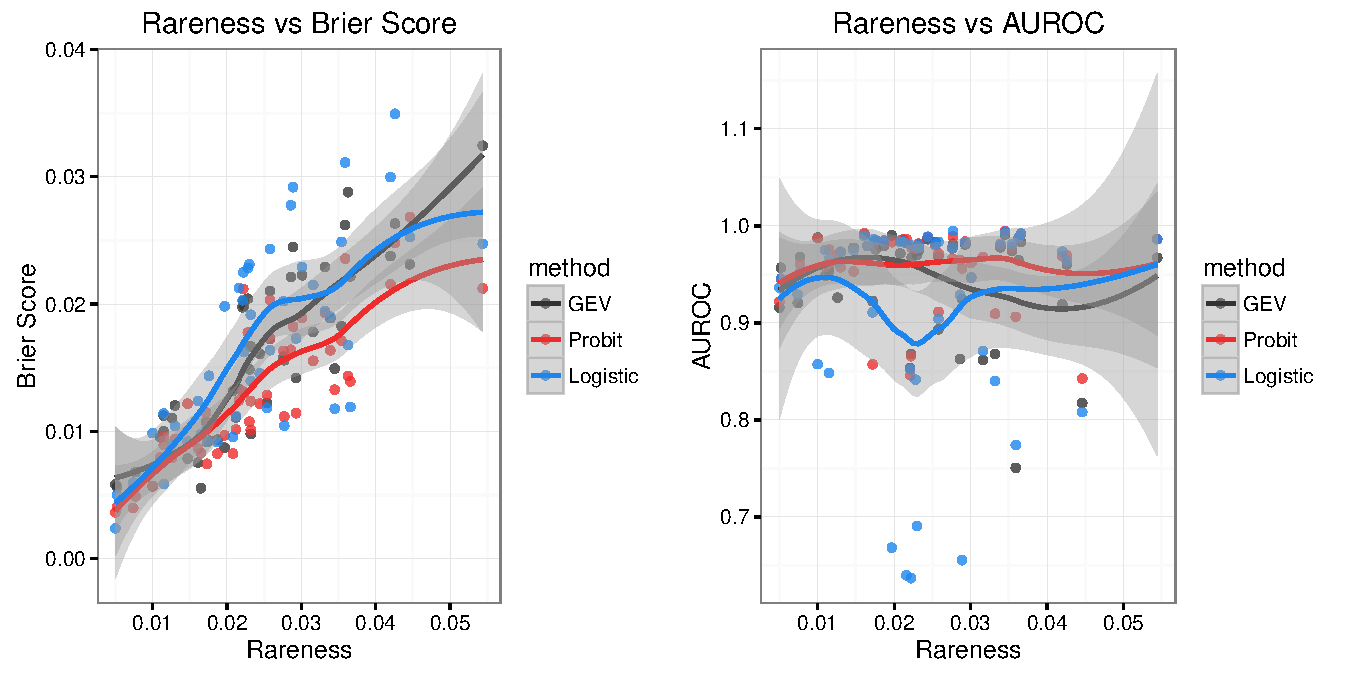
\includegraphics[width=0.47\linewidth]{plots/byrareness-12}
	\caption{Smooth of AUROC by rareness for each sample technique for the hotspot link.}
	\label{rbfig:simsmooth-hot}
\end{figure}

\begin{table}
	\caption{Brier scores ($\times 100$) [SE] and AUROC [SE] for GEV, Probit, and Logistic methods from the simulation study.}
	\label{rbtbl:simbsresults}
	\centering
	\scriptsize
	\begin{tabular}{c c c ccc c ccc}
		\toprule
		\multicolumn{3}{c}{ }& \multicolumn{3}{c}{BS} && \multicolumn{3}{c}{AUROC}\\
		\cmidrule{4-6} \cmidrule{8-10}
		Setting & $n$ & Sample & GEV & Probit & Logistic && GEV & Probit & Logistic\\
		\midrule
		GEV & 100 & CLU & 3.10 [0.27] & 2.45 [0.19] & 2.79 [0.25]
		&& 0.926 [0.009] & 0.942 [0.009] & 0.900 [0.020]\\
		&     & SRS & 2.92 [0.20] & 2.54 [0.18] & 2.92 [0.25]
		&& 0.938 [0.007] & 0.951 [0.007] & 0.879 [0.021]\\
		& 250 & CLU & 2.18 [0.15] & 1.87 [0.13] & 2.05 [0.14]
		&& 0.951 [0.008] & 0.948 [0.011] & 0.922 [0.017]\\
		&     & SRS & 2.29 [0.15] & 2.06 [0.13] & 2.26 [0.15]
		&& 0.949 [0.009] & 0.949 [0.010] & 0.908 [0.020]\\
		\midrule
		Logistic & 100 & CLU & 5.29 [0.25] & 4.94 [0.23] & 5.10 [0.25]
		&& 0.659 [0.012] & 0.676 [0.014] & 0.643 [0.013]\\
		&     & SRS & 5.32 [0.23] & 5.09 [0.24] & 5.34 [0.26]
		&& 0.690 [0.012] & 0.693 [0.012] & 0.613 [0.012]\\
		& 250 & CLU & 4.81 [0.21] & 4.55 [0.21] & 4.66 [0.22]
		&& 0.731 [0.010] & 0.749 [0.010] & 0.714 [0.014]\\
		&     & SRS & 4.86 [0.22] & 4.63 [0.20] & 5.01 [0.23]
		&& 0.742 [0.010] & 0.760 [0.010] & 0.698 [0.015]\\
		\midrule
		Hotspot & 100 & CLU & 2.29 [0.17] & 2.01 [0.15] & 1.81 [0.12]
		&& 0.841 [0.016] & 0.833 [0.019] & 0.824 [0.020]\\
		&     & SRS & 2.09 [0.13] & 1.87 [0.12] & 2.13 [0.15]
		&& 0.885 [0.015] &  0.906 [0.013] & 0.844 [0.015]\\
		& 250 & CLU & 1.65 [0.11] & 1.25 [0.08] & 1.40 [0.09]
		&& 0.934 [0.009] &  0.949 [0.008] & 0.939 [0.011]\\
		&     & SRS & 1.53 [0.10] & 1.31 [0.08] & 1.63 [0.11]
		&& 0.947 [0.007] &  0.960 [0.005] & 0.918 [0.015]\\
		\bottomrule
	\end{tabular}
\end{table}

%\begin{figure}
%  % code/analysis/simstudy/combine-tables.R
%  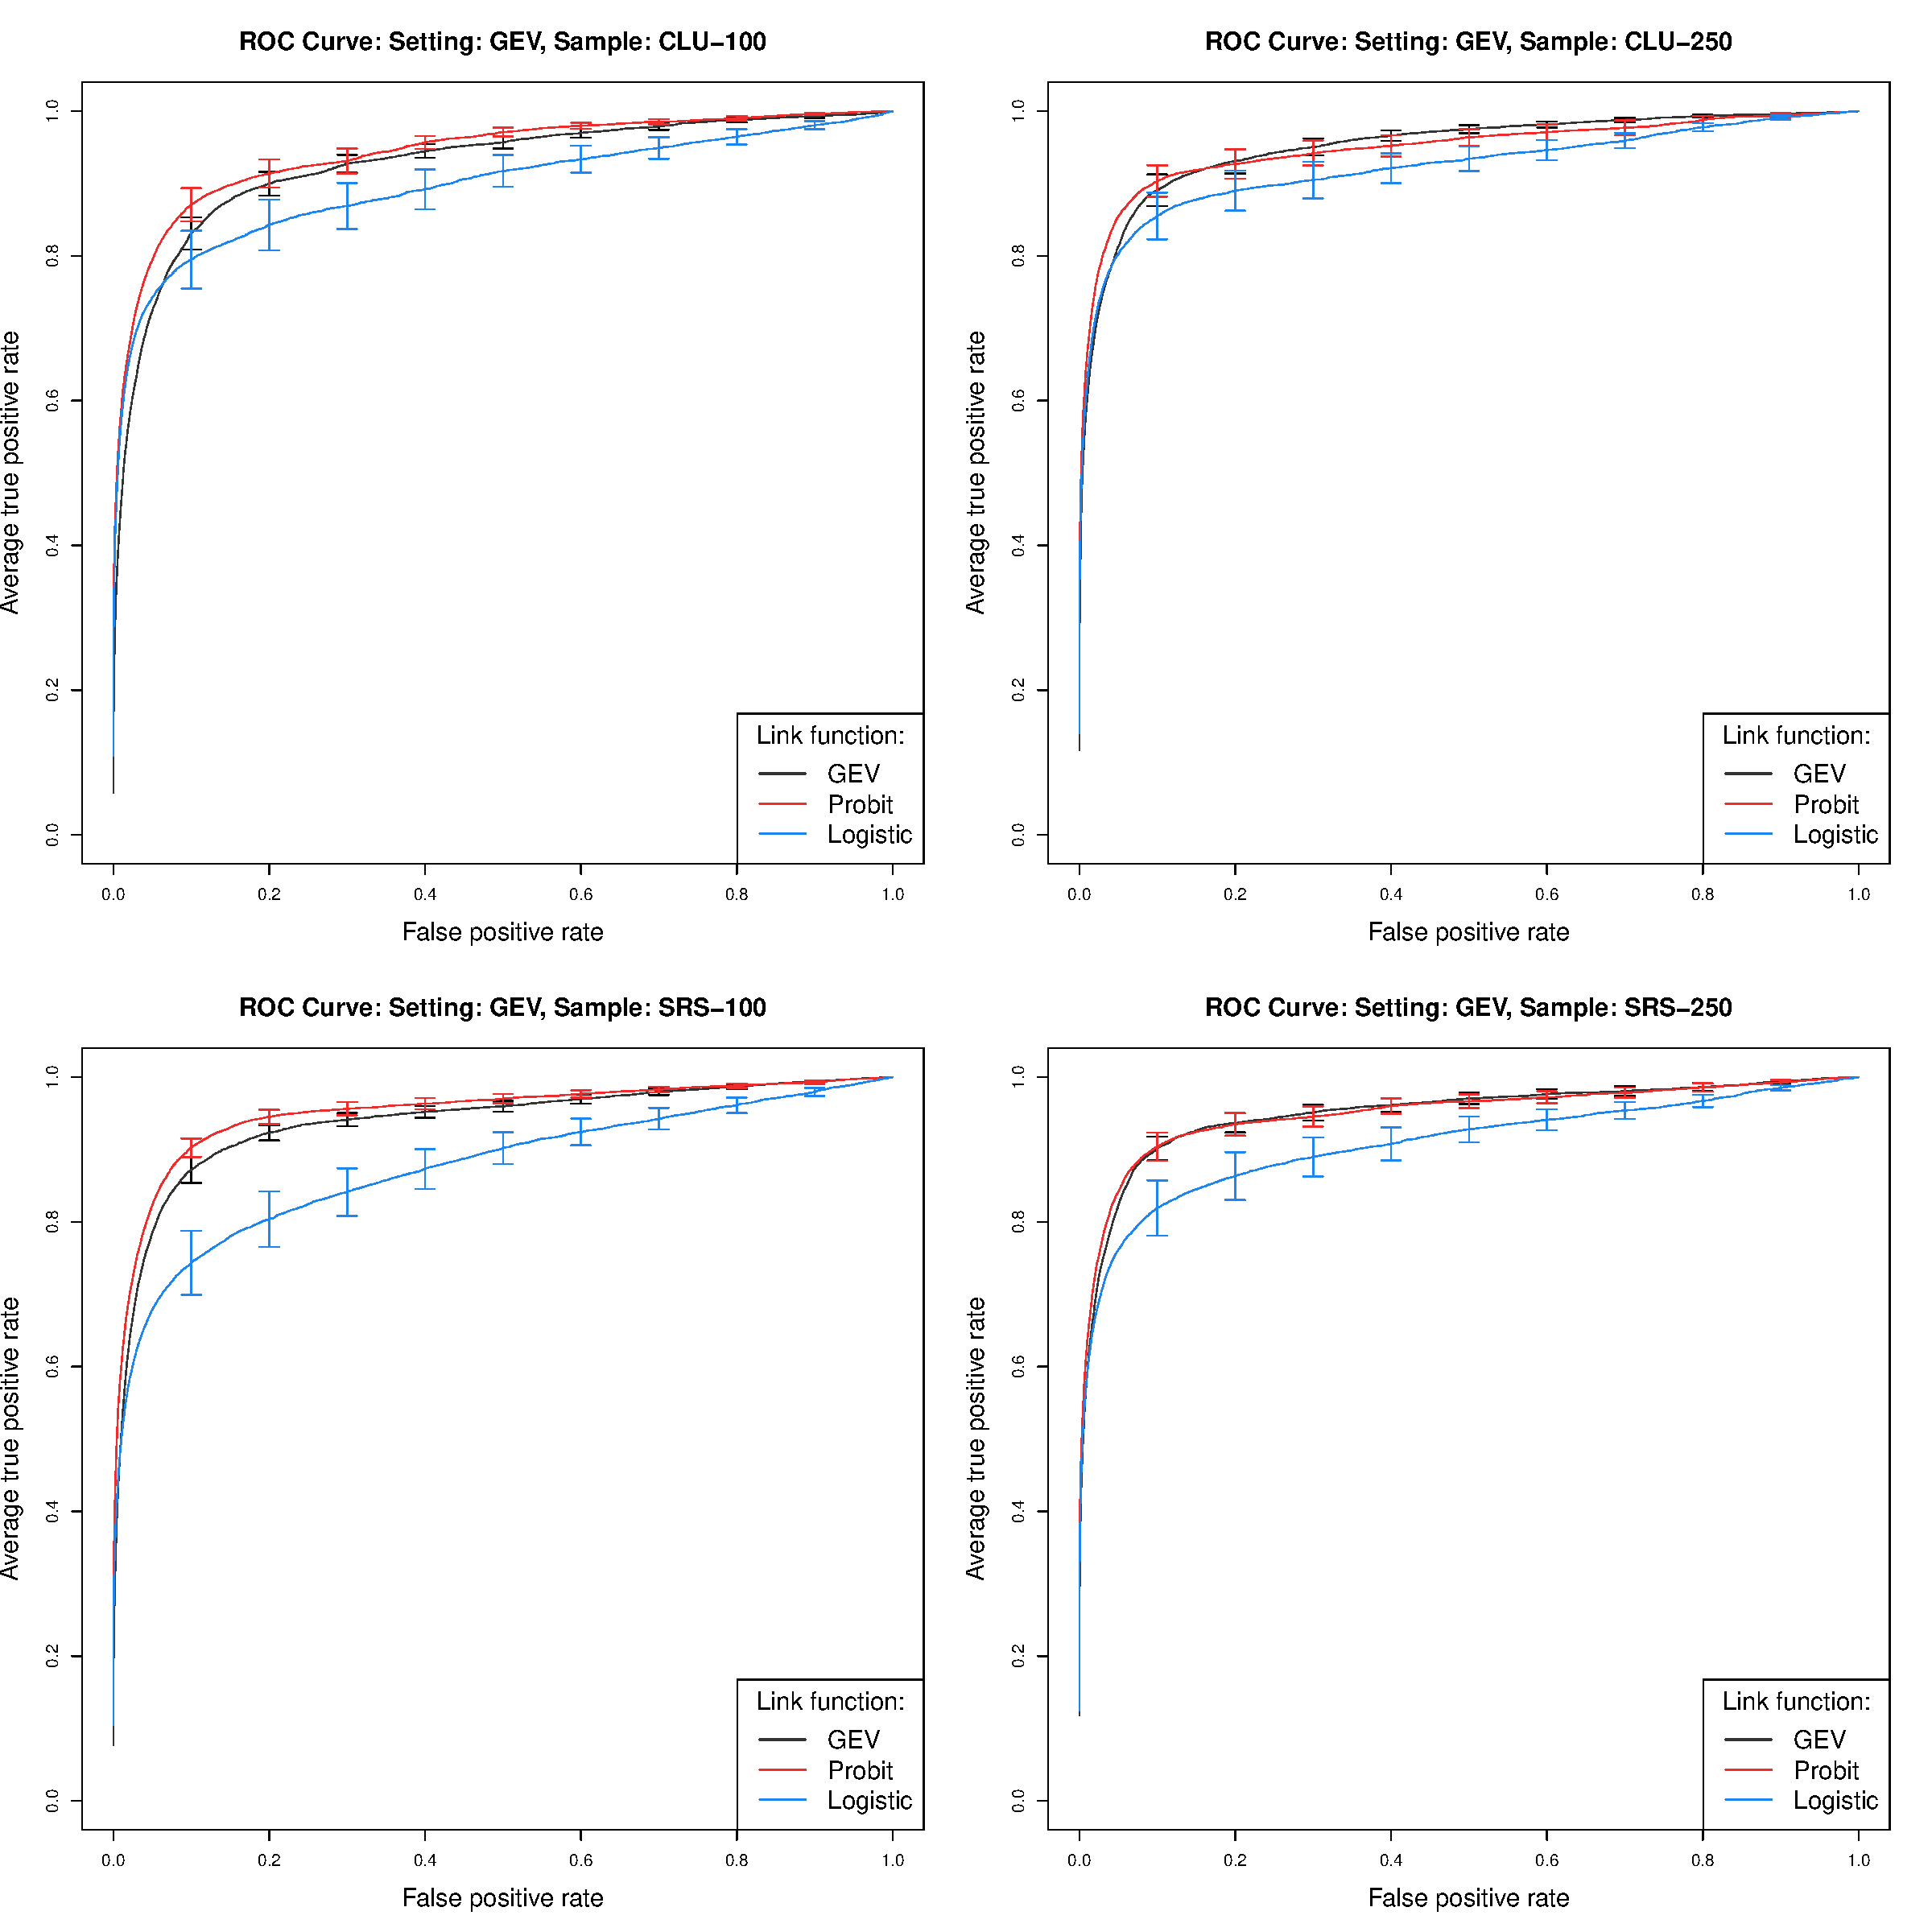
\includegraphics[width=\linewidth]{plots/sim-perf-gev}
%  \caption{Vertically averaged ROC curves for GEV simulation setting.}
%  \label{rbfig:simrocgev}
%\end{figure}
%
%\begin{figure}
%  % code/analysis/simstudy/combine-tables.R
%  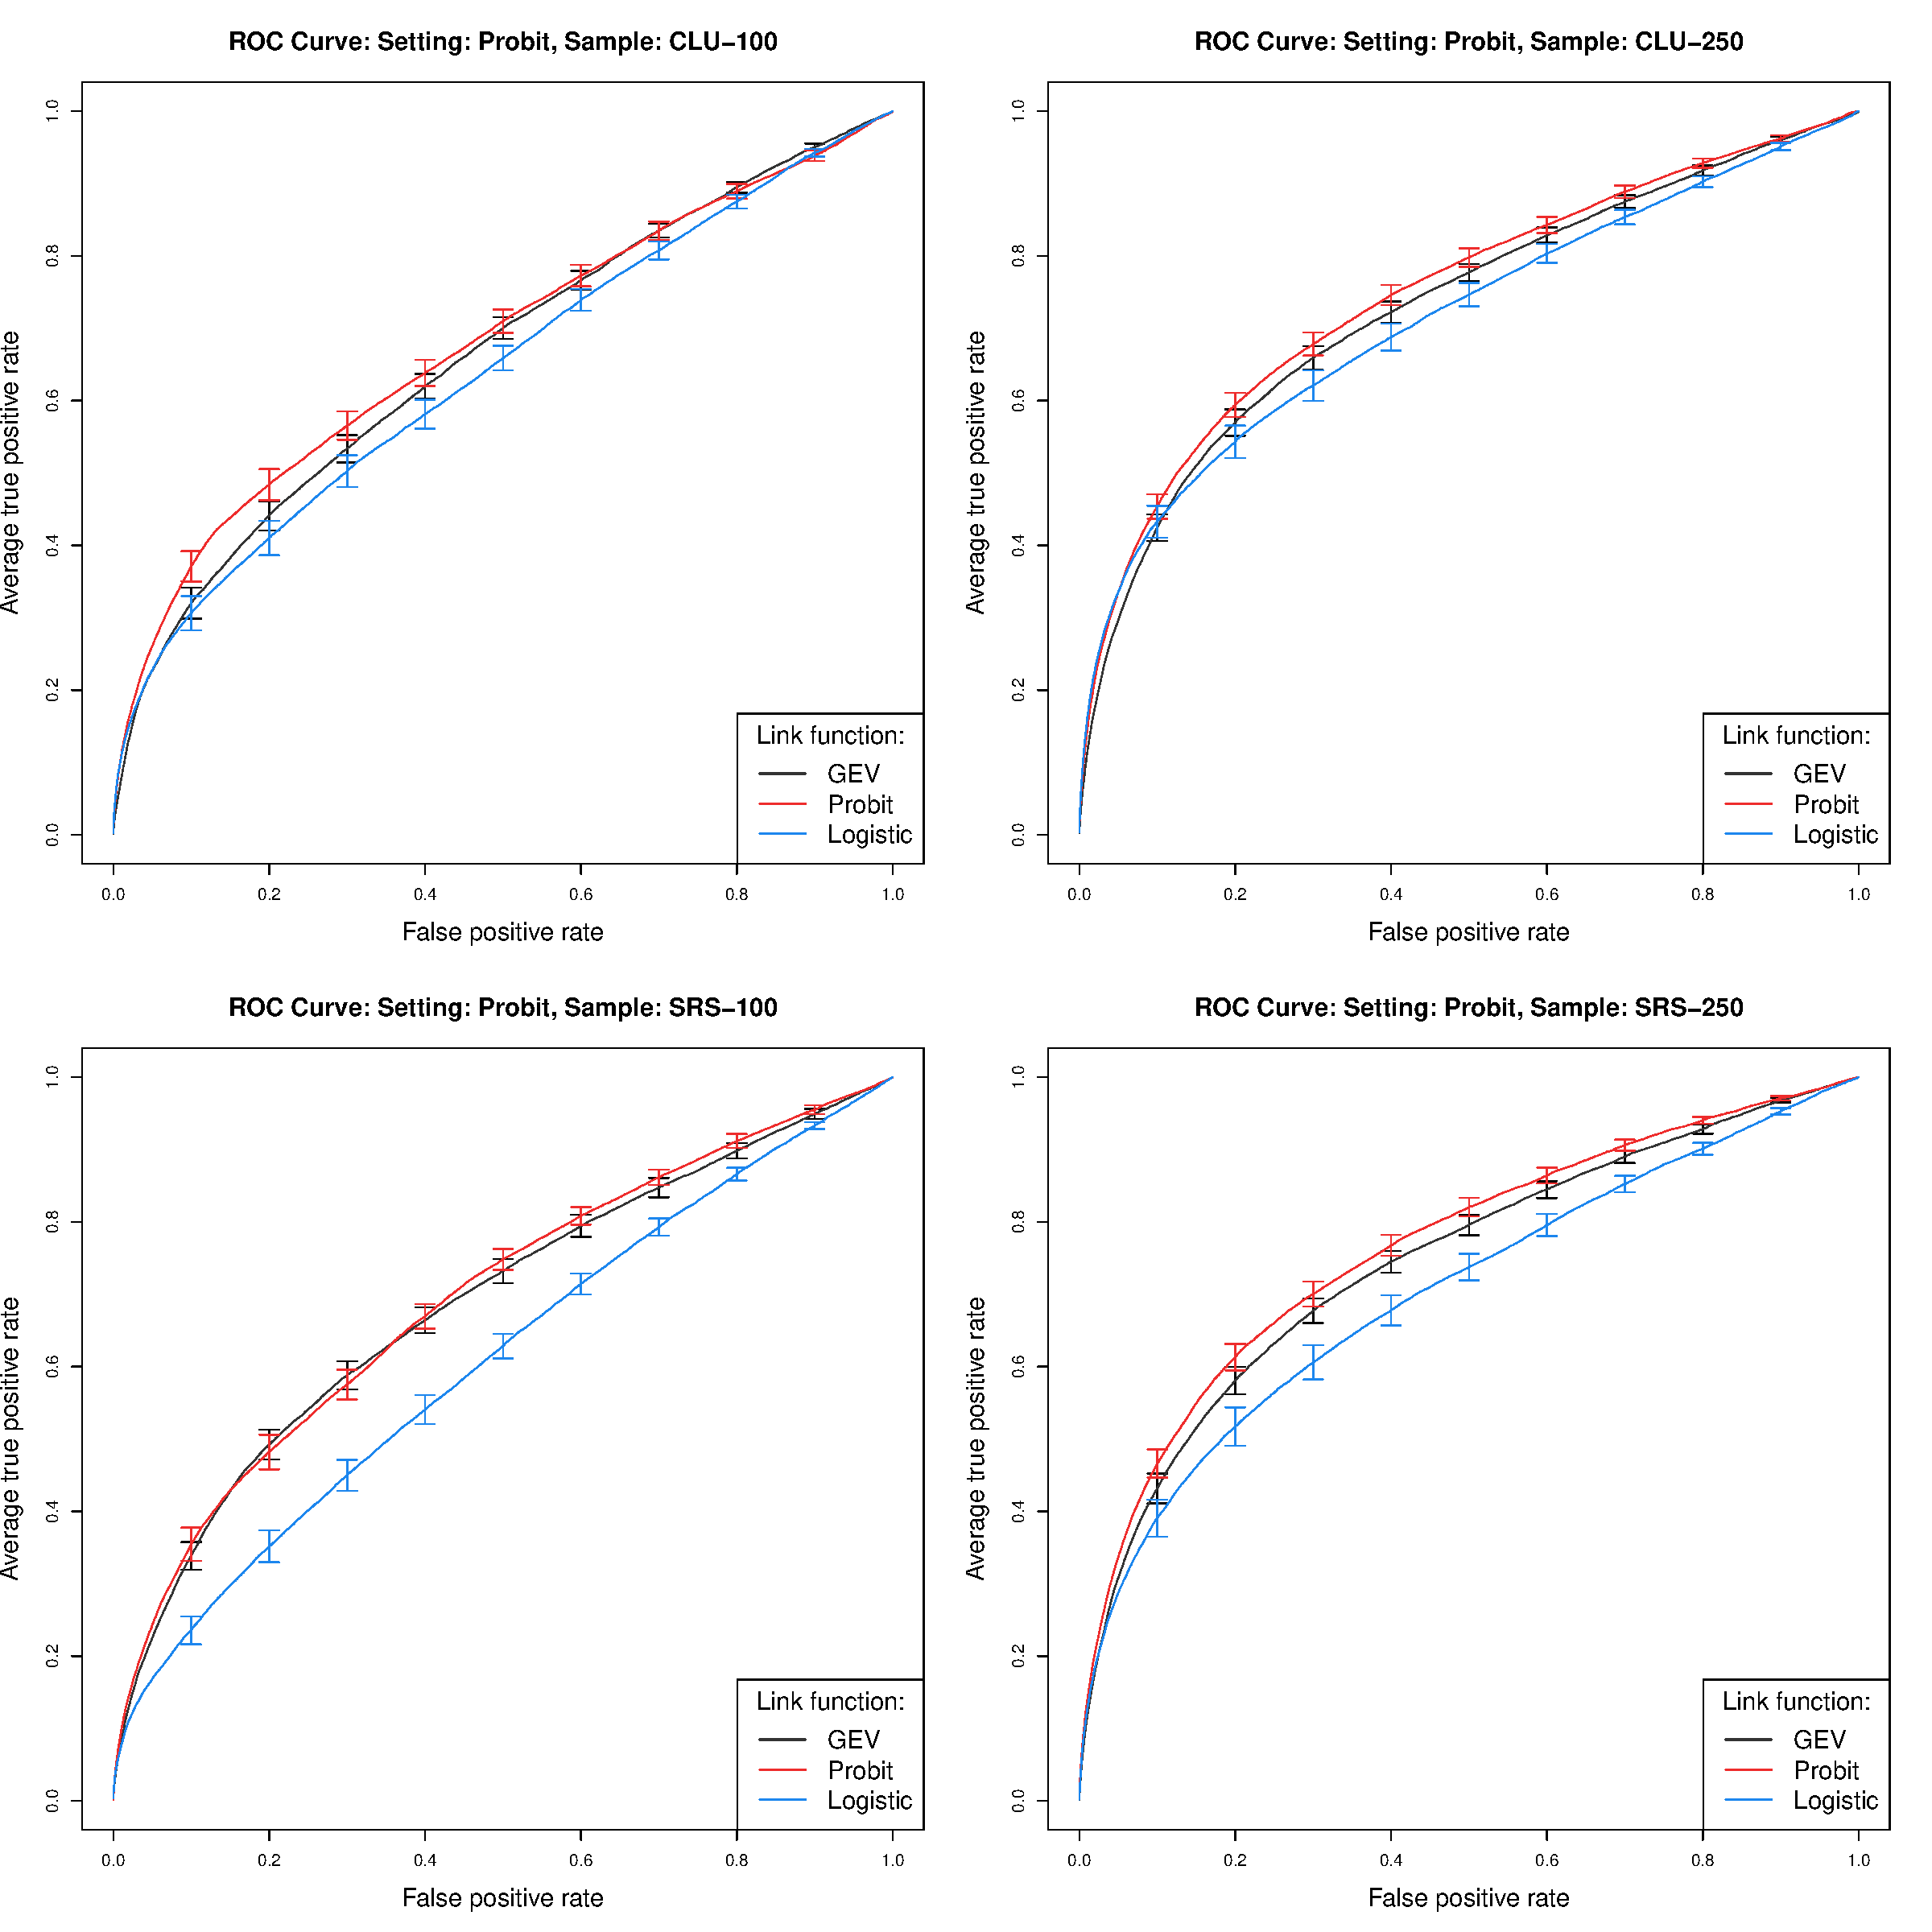
\includegraphics[width=\linewidth]{plots/sim-perf-probit}
%  \caption{Vertically averaged ROC curves for probit simulation setting.}
%  \label{rbfig:simrocpro}
%\end{figure}
%
%\begin{figure}
%  % code/analysis/simstudy/combine-tables.R
%  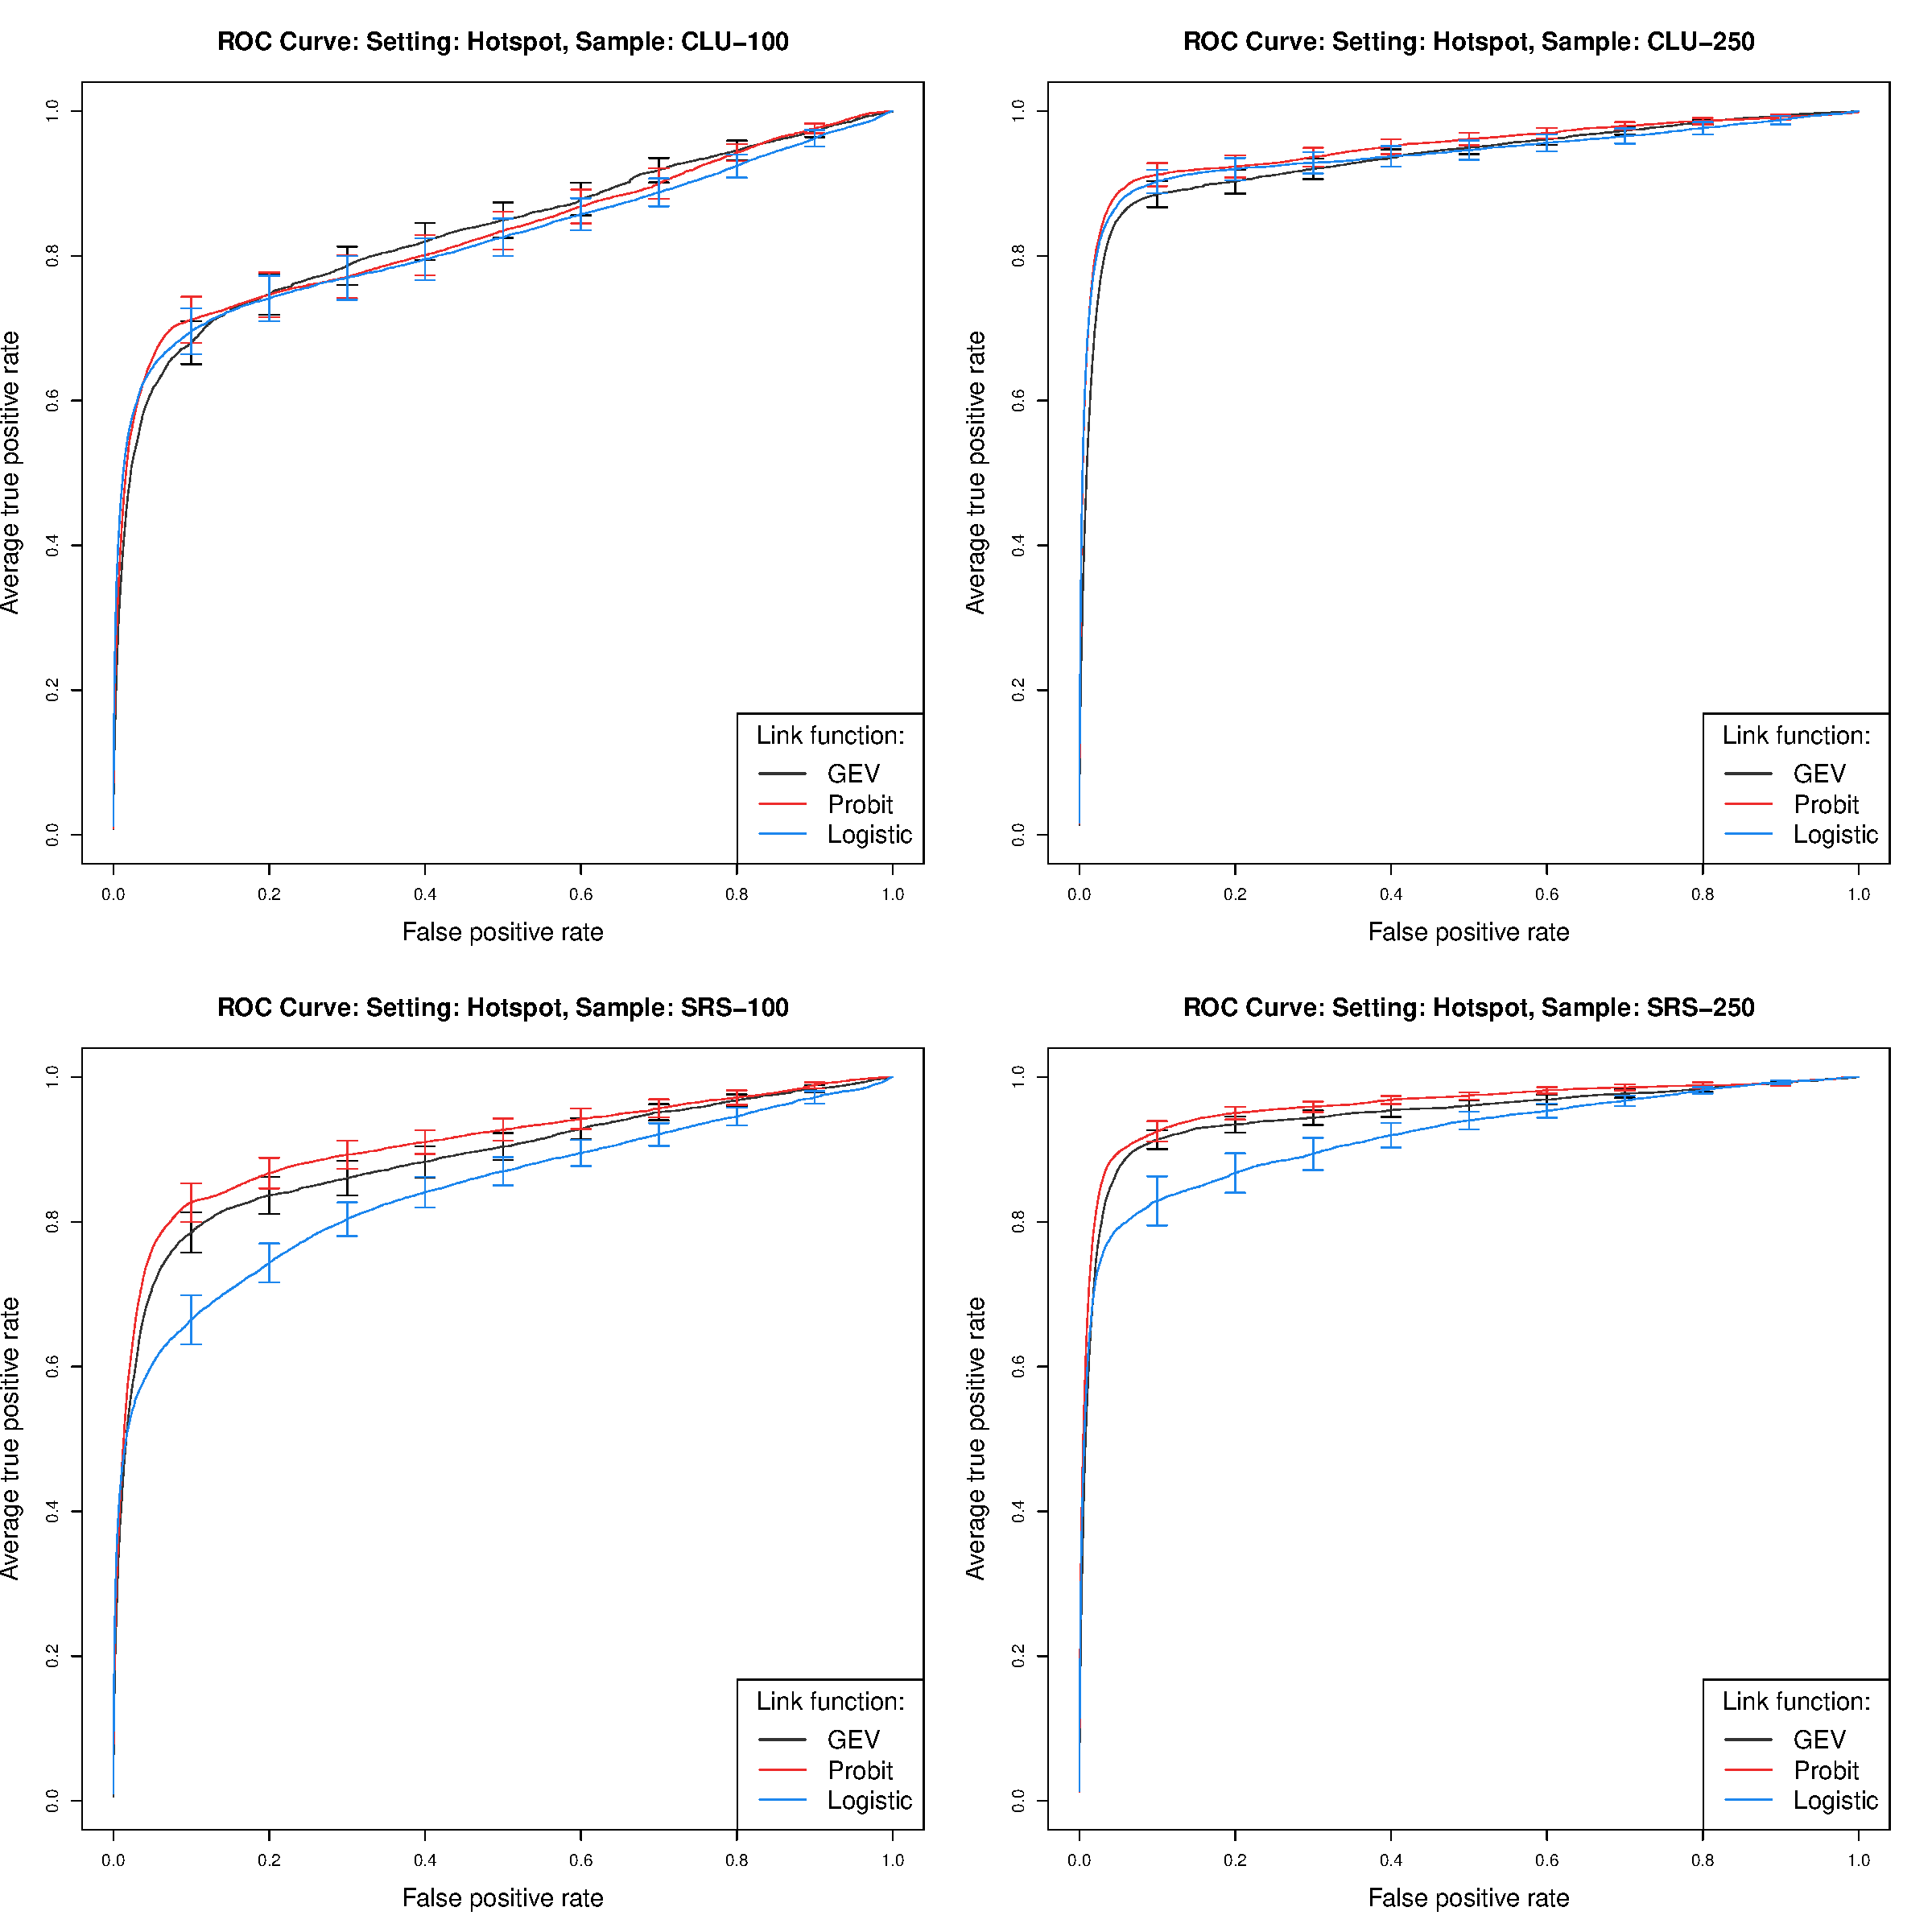
\includegraphics[width=\linewidth]{plots/sim-perf-hotspot}
%  \caption{Vertically averaged ROC curves for hotpost simulation setting.}
%  \label{rbfig:simrochot}
%\end{figure}

% \begin{table}
%   \caption{Relative AUC for GEV and Probit methods}
%   \label{rbtbl:simaucresults}
%   \centering
%   \begin{tabular}{r|lll}
%     \cline{2-4}
%               & GEV    & Probit & Logit\\
%     \hline
%     Setting 1 & 0.8998 & 0.8973 & 0.8897\\
%     Setting 2 & 0.9458 & 0.9399 & 0.9356\\
%     Setting 3 & 0.7288 & 0.7371 & 0.7157\\
%     Setting 4 & 0.7906 & 0.8056 & 0.8115\\
%     Setting 5 & 0.8426 & 0.8458 & 0.8388\\
%     Setting 6 & 0.8756 & 0.8686 & 0.8765\\
%     \hline
%   \end{tabular}
% \end{table}

% We analyzed the results for this simulation study using a Friedman test at $\alpha = 0.05$ to see if at least one method had a significantly different Brier score or AUC.
% For any setting that yielded a significant p-value, we conducted a Wilcoxon-Nemenyi-McDonald-Thompson test to see which of the methods had different results.
% The full results for the Wilcoxon-Nemenyi-McDonald-Thompson tests are given in \aref{rba:pdiffs}.
% For all settings, we find significant results for the Friedman test comparing the Brier scores for the methods.
% Specifcally, we see a statistically significant reduction in Brier score using the GEV compared to logit for settings one and two and compared to probit for setting two.
% However, in the other settings, the logit and probit methods tend to perform better than the GEV method.

% The results using AUC are much less conclusive with only settings one and four demonstrating significant differences between the methods at $\alpha = 0.05$.
% As with the Brier scores, the GEV method shows a statistically significant increase in AUC over the logit method for setting one, and for setting four, the both the probit and logit methods show a statistically significant improvement in AUC over the GEV method.

% \fref{rbfig:post-med-2} and \fref{rbfig:post-med-3} show the posterior median of $P(Y =1)$ for settings 2 and 3 respectively of a simulated dataset.
% As you can see on the figures, the both the spatial probit and logistic models oversmooth $P(Y = 1)$, whereas the spatial GEV method is able to capture small pockets of spatial dependence.
% Plots for the medians of settings 1 and 4 look similar, so they are not included here.

% \begin{figure}
%   % this figure comes from markdown/sim-hmc/predict-maps.R
%   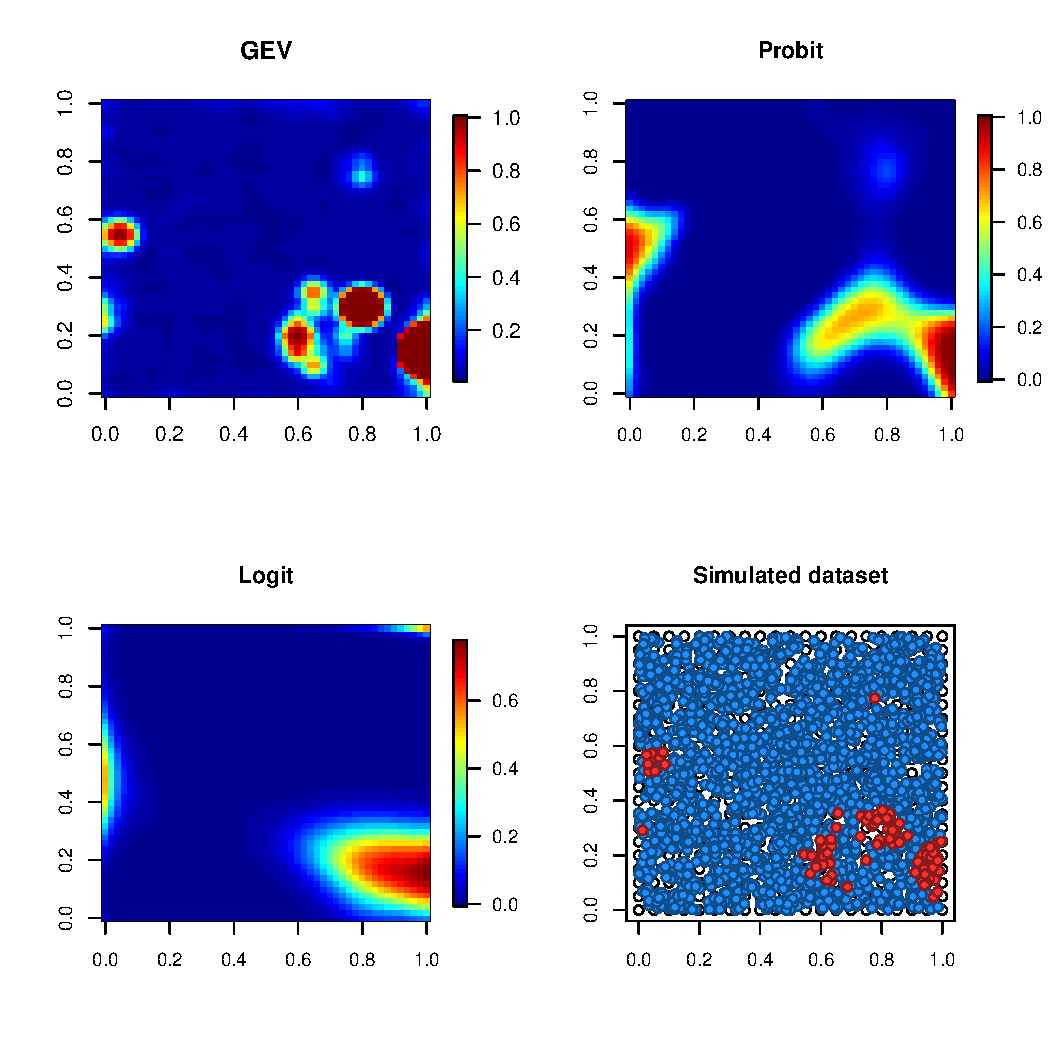
\includegraphics[width=\linewidth]{plots/post-med-2.pdf}
%   \caption{Posterior median $P(Y = 1)$ for spatial GEV, probit, and logistic regression for setting 2.}
%   \label{rbfig:post-med-2}
% \end{figure}

% \begin{figure}
%   % this figure comes from markdown/sim-hmc/predict-maps.R
%   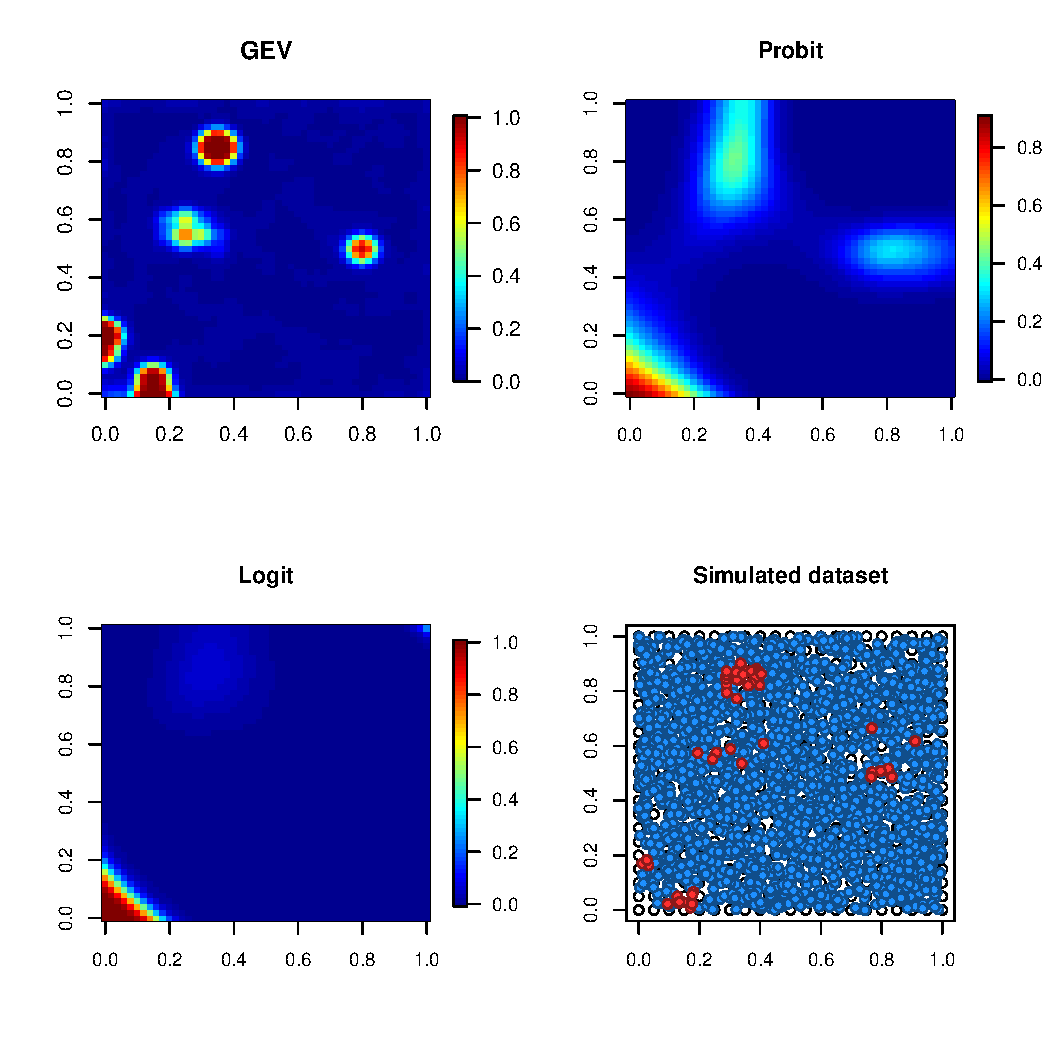
\includegraphics[width=\linewidth]{plots/post-med-3.pdf}
%   \caption{Posterior median $P(Y = 1)$ for spatial GEV, probit, and logistic regression for setting 3.}
%   \label{rbfig:post-med-3}
% \end{figure}

% If needed, species 2 is \emph{Hedysarum scoparium} , and \emph{Hedysarum scoparium} can be found in $0.54\%$ of the grid cells.

\section{Data analysis}\label{rbs:dataanalysis}

We compare our method to the spatial probit and logistic models for mapping the probability of the occurrence of \tamarix{} (TR) and \hedysarum{} (HS), two  plant species, for a 1-km$^2$ study region of PR China \citep{Smith2012}.
The Chinese Academy of Forestry conducted a full census of the area, and the true occupancy of the species are plotted in \fref{rbfig:occupancy}.
\begin{figure}
	\centering
	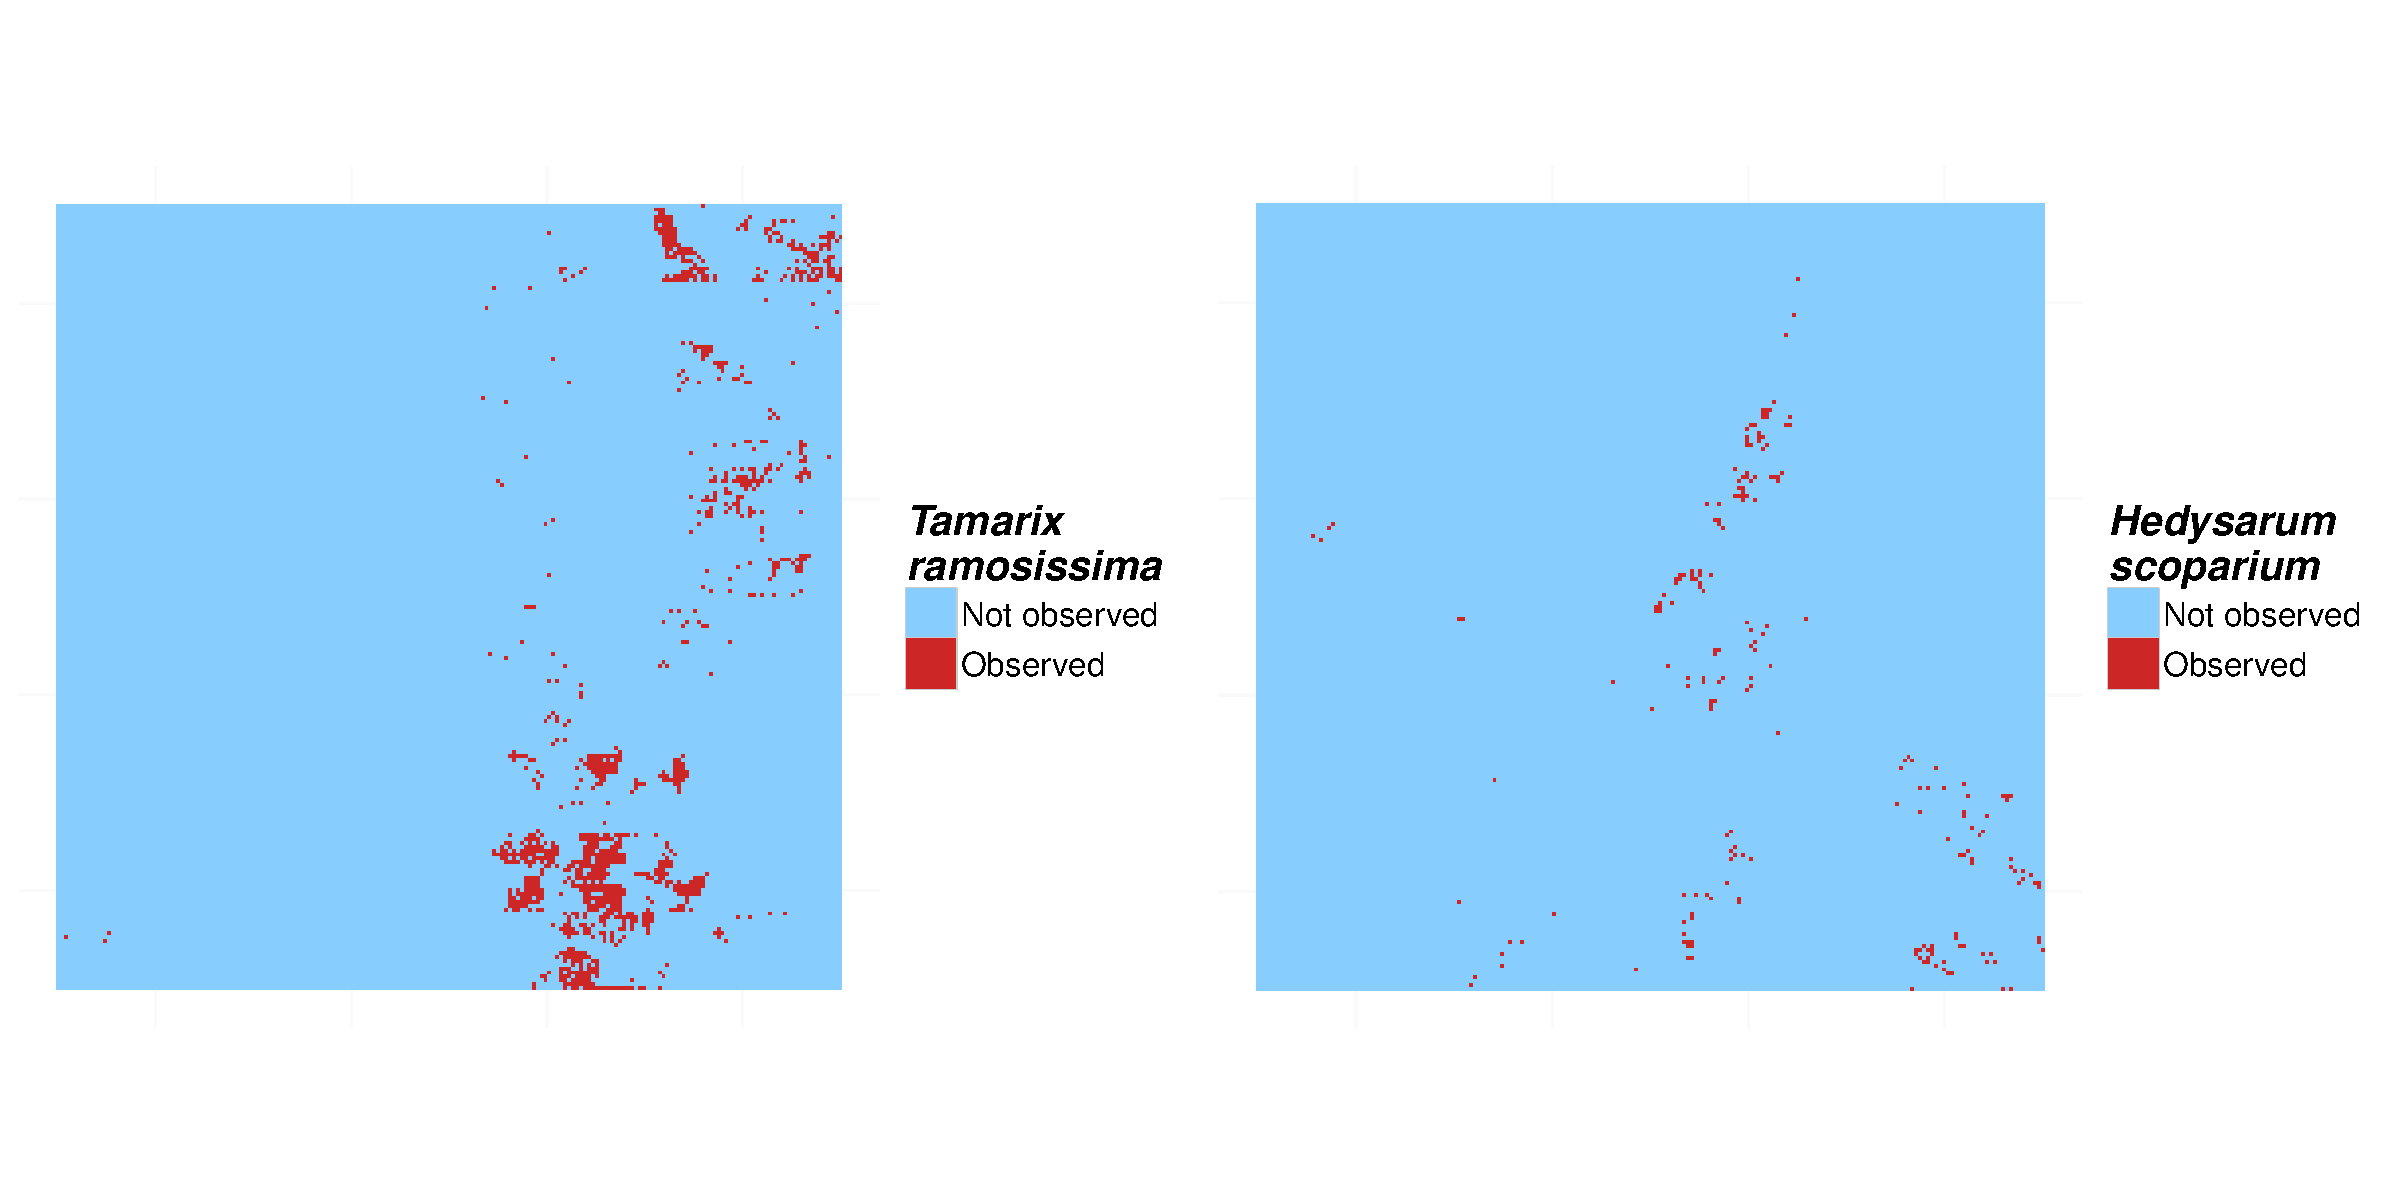
\includegraphics[width=\linewidth, trim=0 10em 0 10em]{plots/plant-census.pdf}
	\caption{True occupancy of \tamarix{} (left) and \hedysarum{} (right) from a 1-km$^2$ study region of PR China.}
	\label{rbfig:occupancy}
\end{figure}
The region is split into $10$-m $\times$ $10$-m grid cells.
\tamarix{} can be found in approximately $6\%$ of the grid cells, and \hedysarum{} can be found in approximately $0.54\%$ of the grid cells.

\subsection{Methods} \label{rbs:datamethods}

For the data analysis, we generate 50 subsamples using the CLU and SRS sampling methods with $n_s = 100$, $250$ initial locations.
For each subsample, we fit the spatial GEV, spatial probit, and spatial logistic models.
Knot placement, prior distributions, and MCMC details for the data analysis are the same as the simulation study.
To compare models, we use similar metrics as in the simulation study, but we average the metrics over subsamples.

\subsection{Results}\label{rbs:dataresults}

The results of the real data analysis mirror those of the simulation study.
\tref{rbtbl:dataresults} gives summary Brier scores ($\times 100$) and AUROC for the \tamarix{} and \hedysarum{} analysis along with the time (in seconds) for 1,000 iterations of the MCMC sampler.
These timings come from a single core of an Intel Core i7-5820K Haswell-E processor, using the OpenBLAS optimized BLAS library (\url{http://www.openblas.net}).
\fref{rbfig:data1roc} gives the vertically averaged ROC curves for each method and sampling setting for \tamarix{} and \fref{rbfig:data2roc} gives the vertically averaged ROC curves for \hedysarum{}.
These results appear to support the suggestion from the simulation study that spatial GEV gives an advantage as rareness increases.
For \tamarix, when $n = 100$, there is a small distinction between the spatial GEV and probit models.
The results suggest that the GEV model has a small improvement over probit in the case of cluster sampling, but that using a probit model demonstrates a small improvement over the GEV model in the simple random setting.
However, when $n = 250$, both logistic and probit models appear to outperform the GEV model.
For the rarer species, \hedysarum, we find more conclusive evidence that the GEV model provides an improvement for cluster sampling when $n = 100$.
At this sample size, there is also some evidence to suggest that the GEV model gives some improvement over the probit model for simple random sampling.
For $n = 250$, we have evidence that using a cluster sampling strategy, the GEV model gives the best performance, but for simple random sampling, the probit model performs the best.

\section{Discussion and future research}\label{rbs:conclusions}

In this paper, we present a max-stable spatial method for rare binary data.
The principal finding in this paper is that the spatial probit model is sufficient for binary data except in the most extreme cases with occurring for less than 1\% of the observations.
This finding is surprising given that the max-stable process is the theoretically justified spatial process for extreme value distributions, and it leads to possible research questions in the future.
Nevertheless, both the probit and GEV models  outperform the logistic method, which is often the default method chosen for analysis of binary data.

It is unusual that the spatial probit model should outperform the proposed model, particularly when the data are generated directly from the proposed model.
One possible explanation is that for the simulated data, there is a wide range of rarity in the data (GEV: $0.5\%$ -- $35.9\%$, Logistic: $1.4\%$ -- $14.4\%$, and Hotspot: $0.5\%$ -- $6.8\%$).
Given that for both the GEV and logistic data settings, we have a number of datasets with a relatively high rate of occurrence, it is possible that probit is competitive partly due to the fact that the data are not rare.
Both the simulation study and data analysis appear to support the idea that the GEV method will perform better on rarer datasets.
Therefore, it may be useful to conduct more research on rare datasets or through simulation with a slightly more restrictive data generation strategy (i.e. restrict datasets to populations that are rarer than $5\%$).

\begin{figure}
	% code/analysis/swd/combine-tables.R
	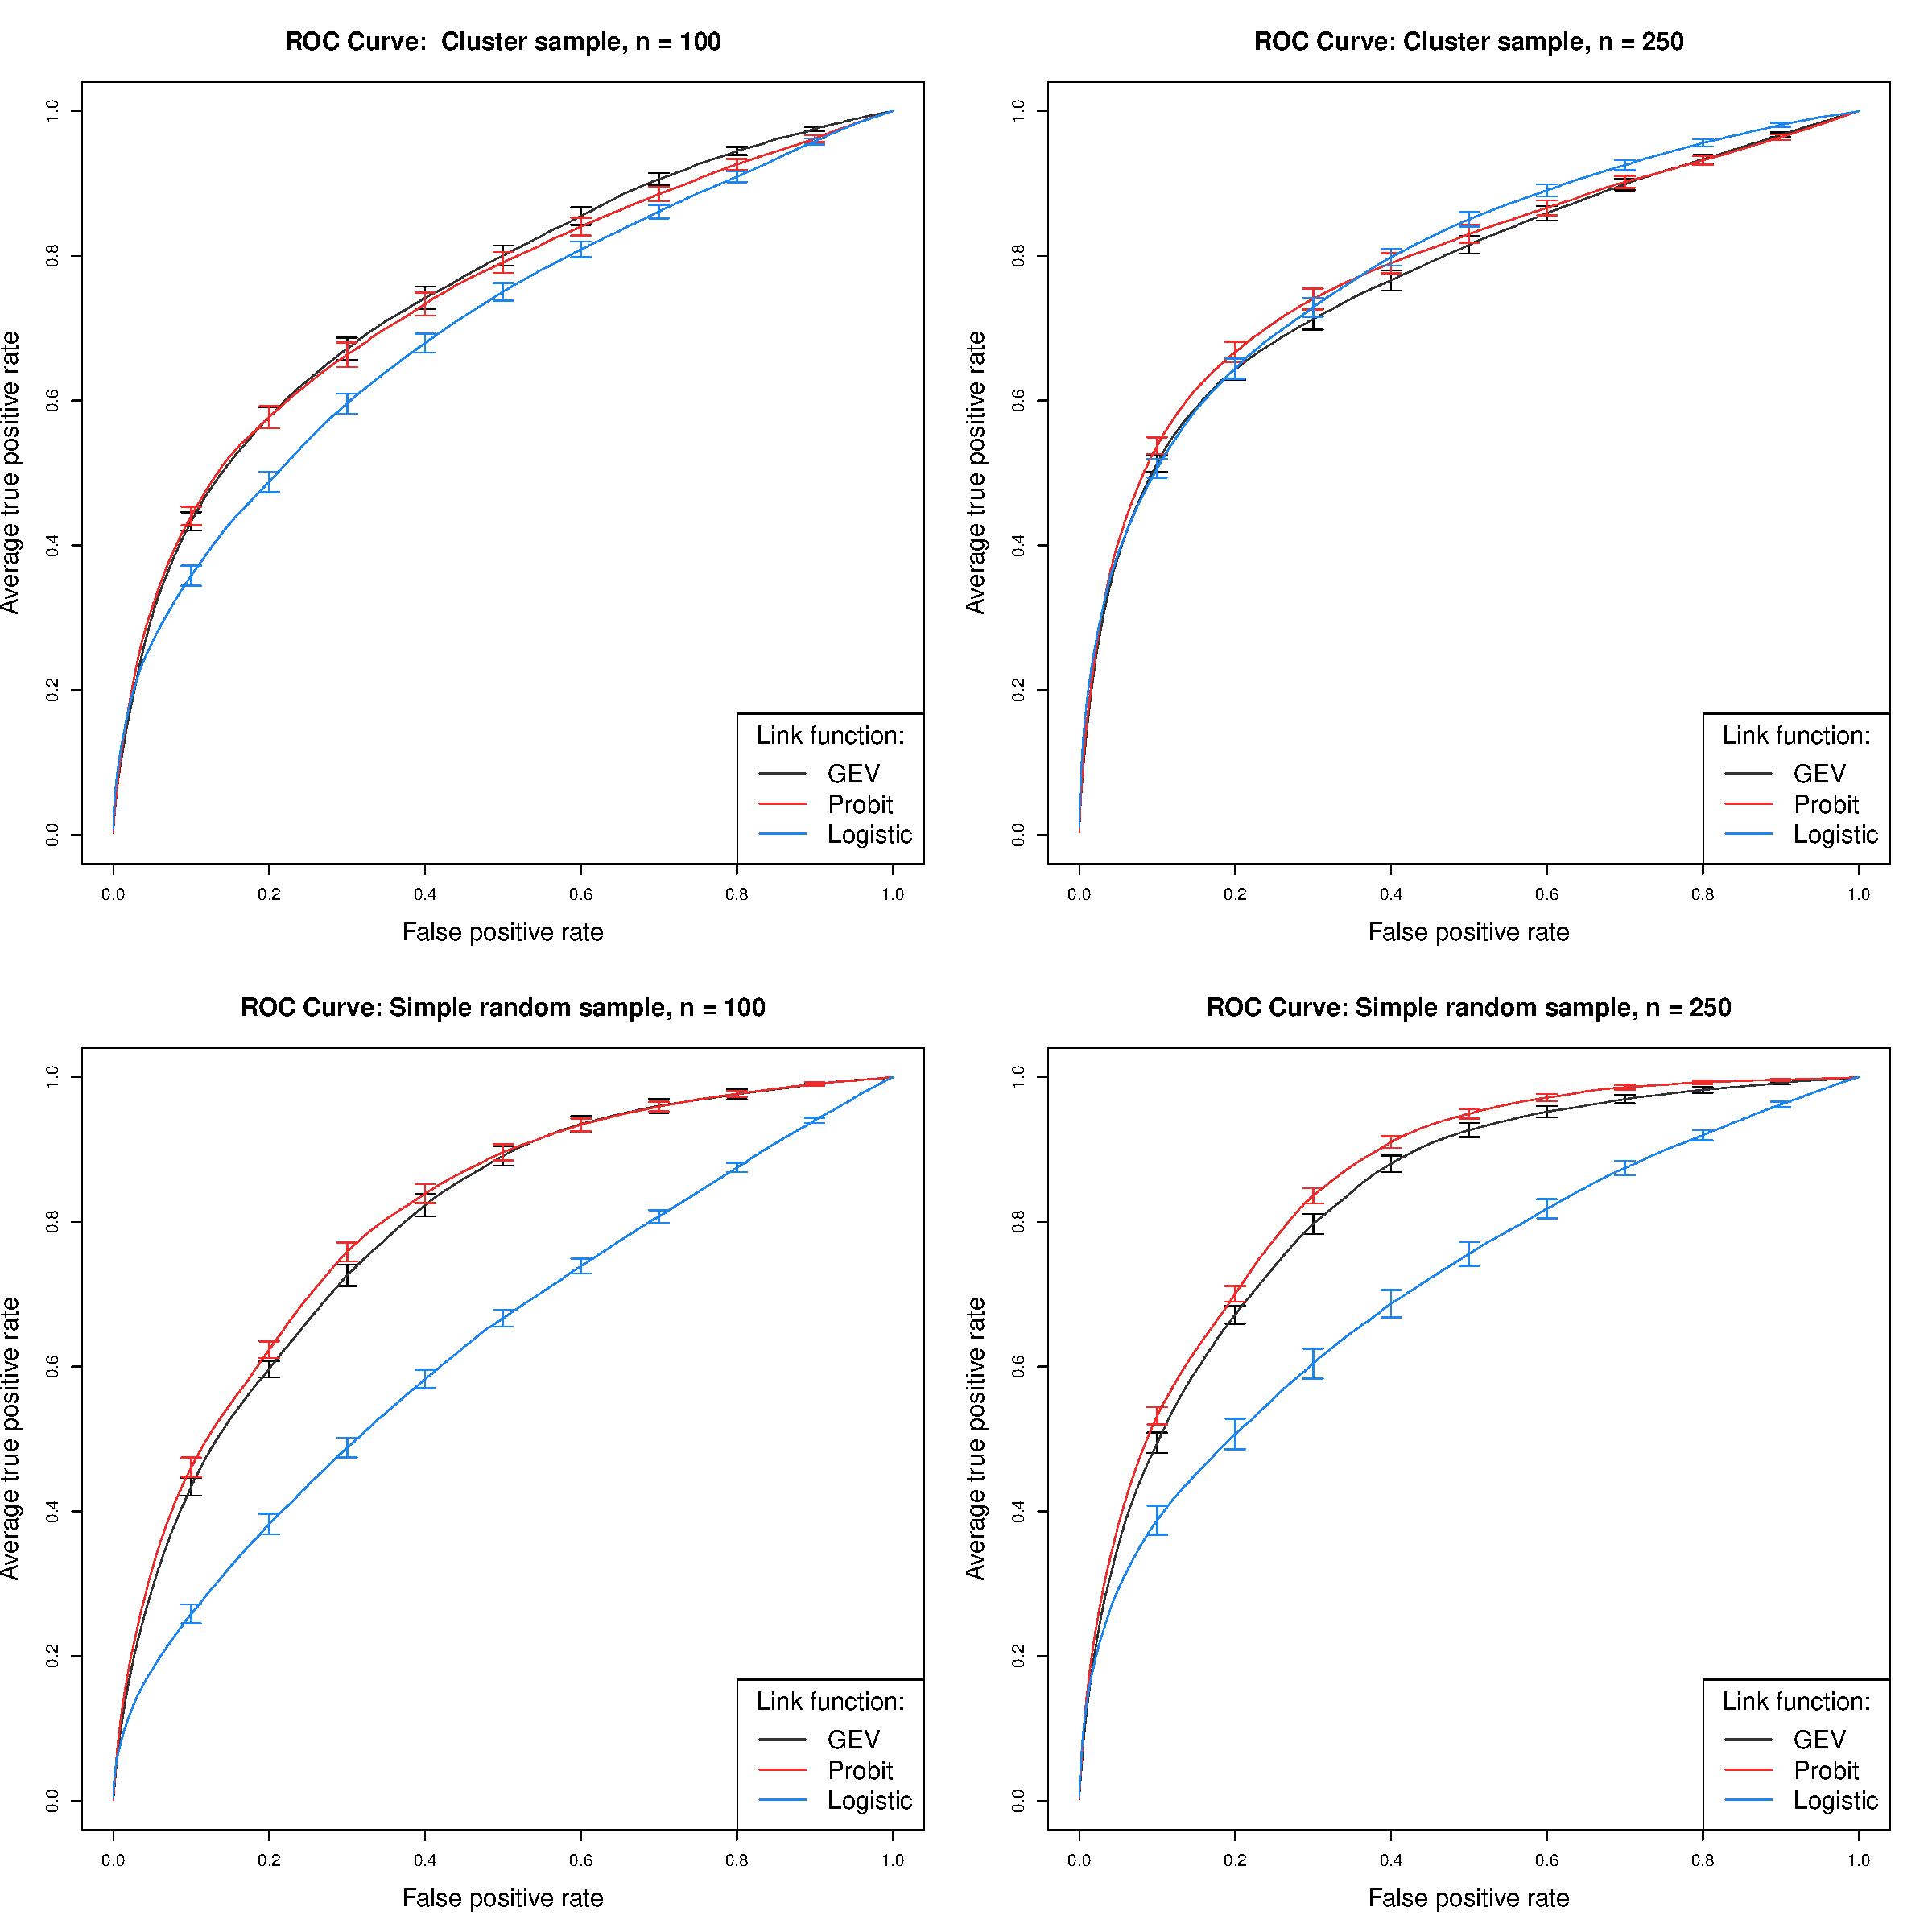
\includegraphics[width=\linewidth]{plots/data-perf-species1}
	\caption{Vertically averaged ROC curves for \tamarix{}.}
	\label{rbfig:data1roc}
\end{figure}

\begin{figure}
	% code/analysis/swd/combine-tables.R
	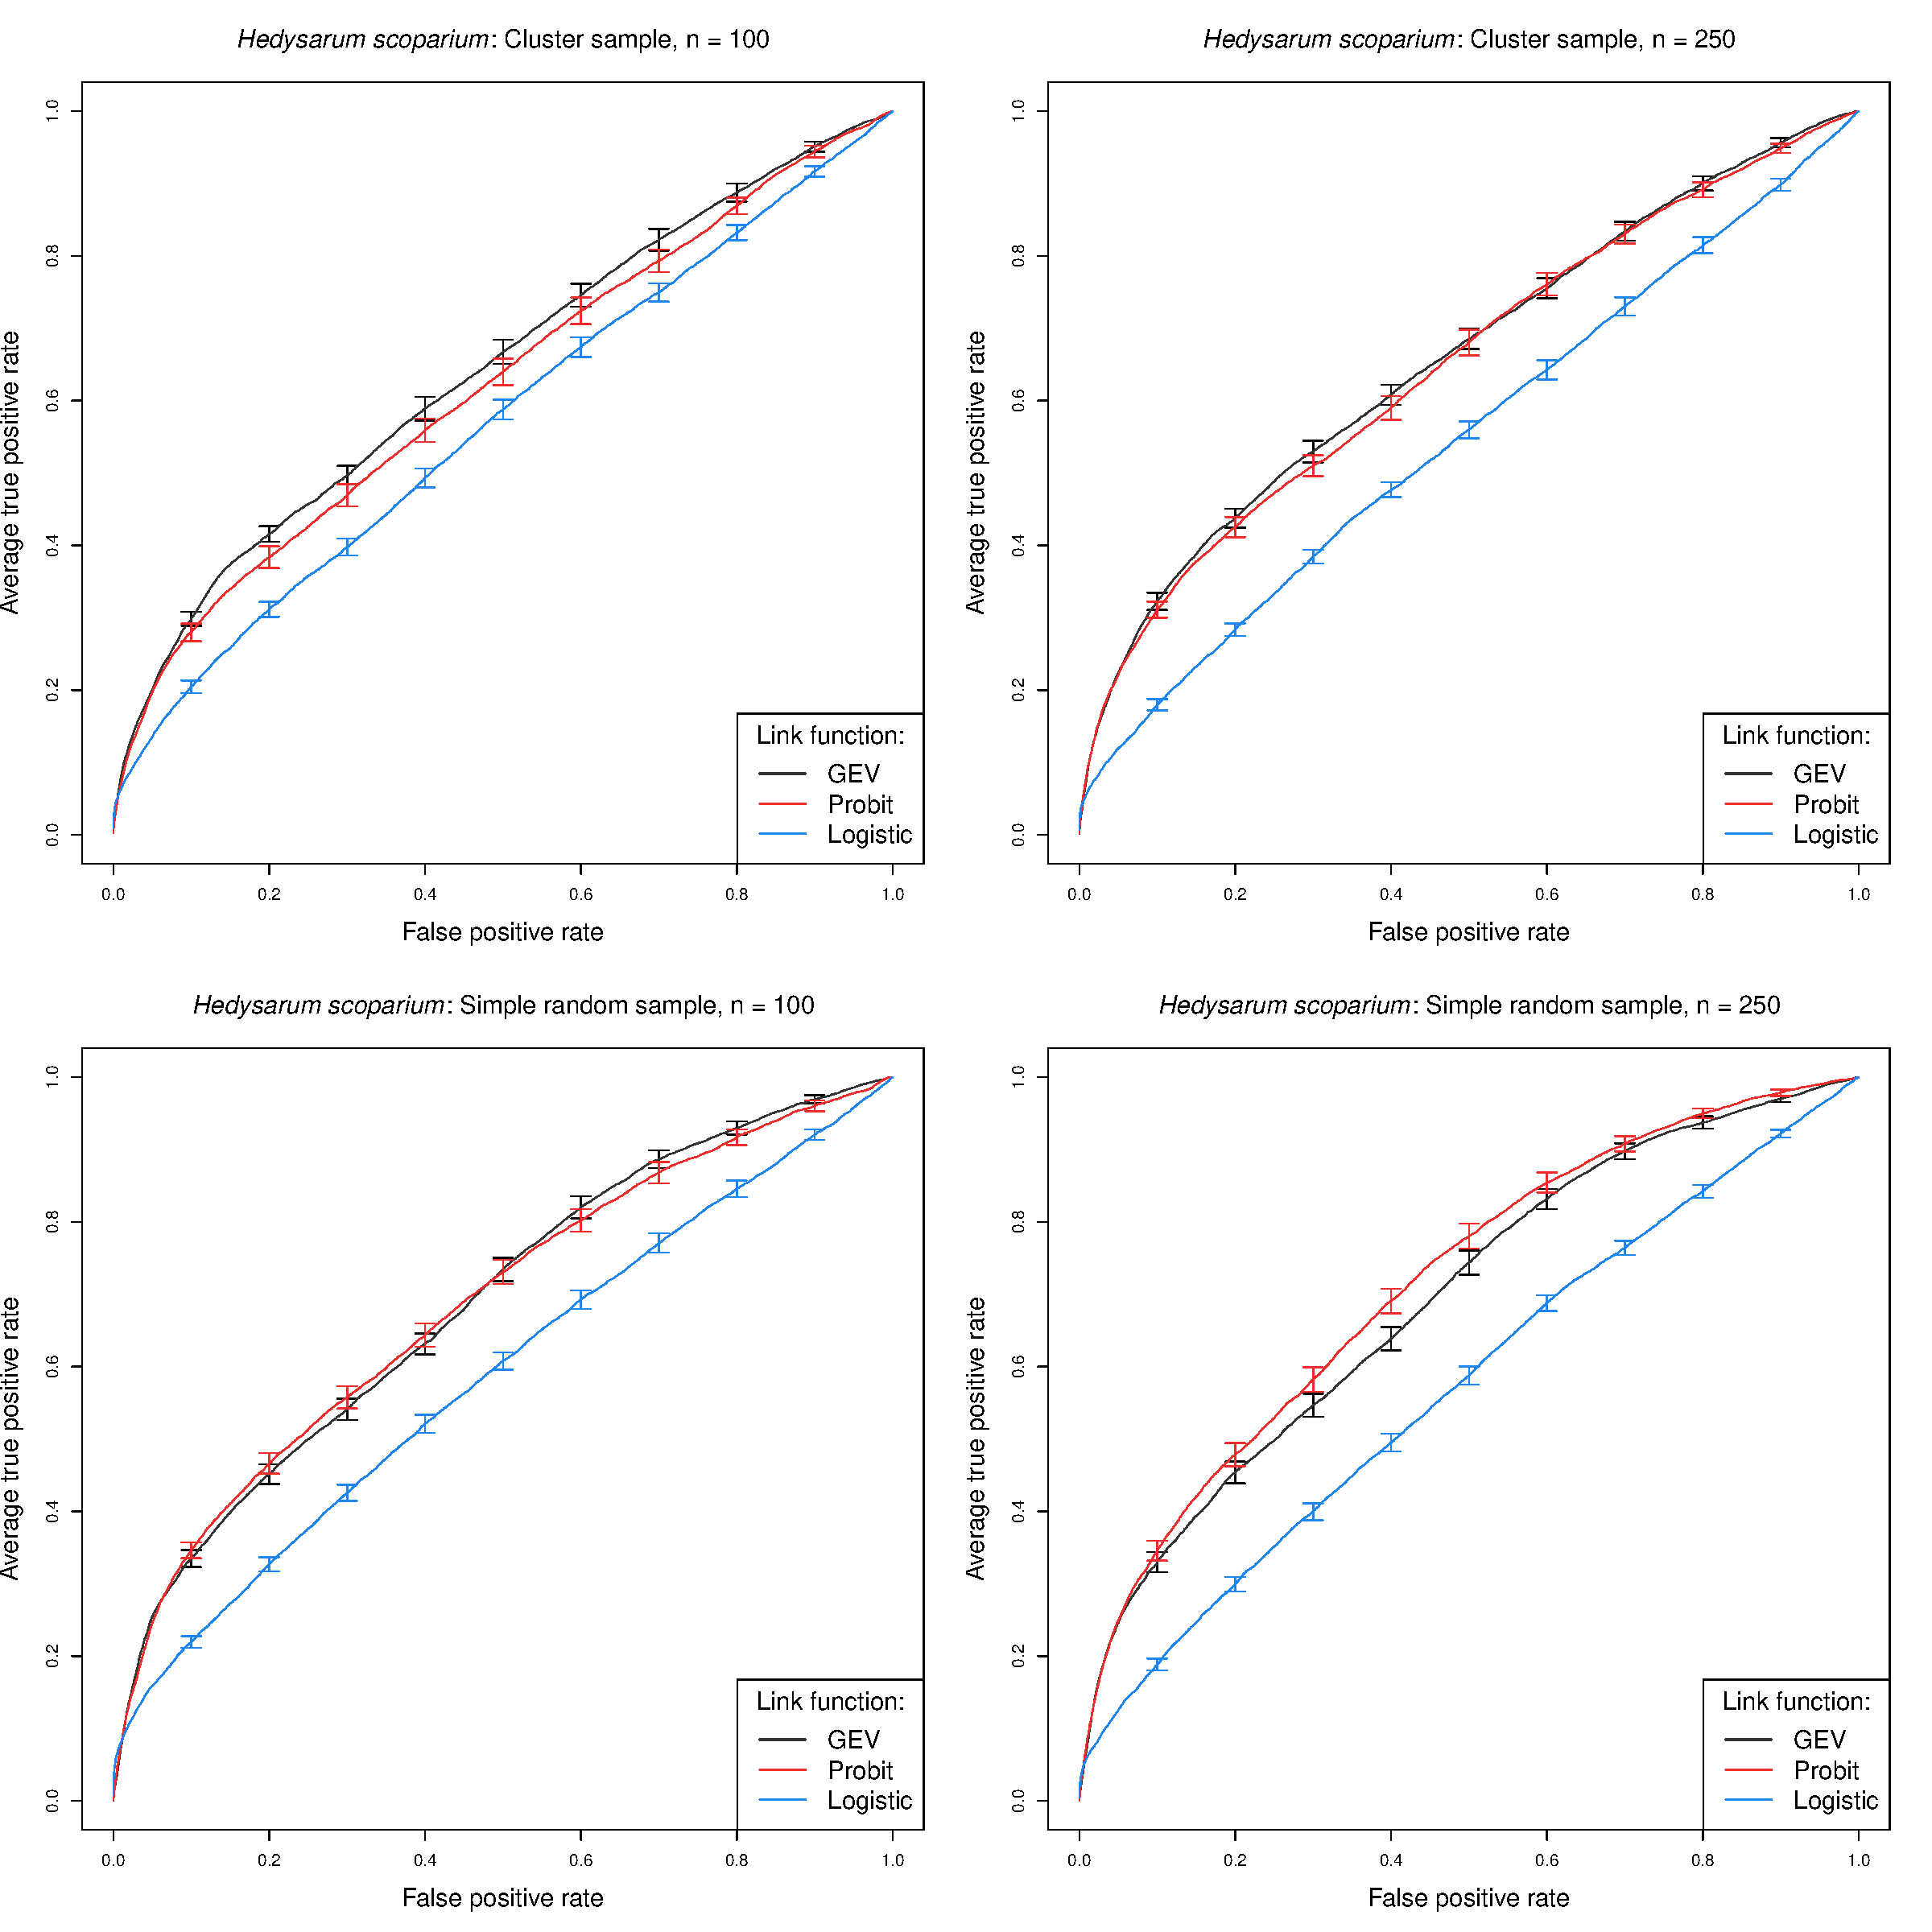
\includegraphics[width=\linewidth]{plots/data-perf-species2}
	\caption{Vertically averaged ROC curves for \hedysarum{}.}
	\label{rbfig:data2roc}
\end{figure}

\begin{landscape}
	\thispagestyle{lscapedplain}
	\begin{table}
		\caption{Brier scores ($\times 100$) [SE], AUROC [SE], and time (in seconds) for 1,000 iterations of GEV, Probit, and Logistic methods for \tamarix{} and \hedysarum{}.}
		\label{rbtbl:dataresults}
		\centering
		\scriptsize
		\subfloat[\tamarix{}]{
			\begin{tabular}{c c ccc c ccc c rrr}
				\toprule
				\multicolumn{2}{c}{ }& \multicolumn{3}{c}{BS} && \multicolumn{3}{c}{AUROC} && \multicolumn{3}{c}{Time} \\
				\cmidrule{3-5} \cmidrule{7-9} \cmidrule{11-13}
				$n$ & Samp. & GEV    & Probit & Logistic && GEV    & Probit & Logistic && GEV    & Probit & Logistic \\
				\midrule
				100 & CLU & 5.120 [0.050] & 5.039 [0.049] & 5.382 [0.029]
				&& 0.732 [0.014] & 0.731 [0.014] & 0.699 [0.012]
				&& 6.1 & 1.1 & 2.4\\
				& SRS & 4.997 [0.045] & 4.938 [0.055] & 5.500 [0.027]
				&& 0.798 [0.008] & 0.802 [0.009] & 0.636 [0.012]
				&& 6.2 & 1.1 & 2.6\\
				250 & CLU & 4.779 [0.049] & 4.657 [0.045] & 4.950 [0.051]
				&& 0.771 [0.013] & 0.784 [0.013] & 0.798 [0.011]
				&& 32.0 & 7.1 & 21.2 \\
				& SRS & 4.823 [0.053] & 4.735 [0.048] & 5.120 [0.071]
				&& 0.827 [0.011] & 0.851 [0.007] & 0.717 [0.019]
				&& 32.6 & 7.0 & 21.0 \\
				\bottomrule
			\end{tabular}
		}

		\subfloat[\hedysarum]{
			\begin{tabular}{c c ccc c ccc c rrr}
				\toprule
				\multicolumn{2}{c}{ }& \multicolumn{3}{c}{BS} && \multicolumn{3}{c}{AUROC} && \multicolumn{3}{c}{Time}\\
				\cmidrule{3-5} \cmidrule{7-9} \cmidrule{11-13}
				$n$ & Samp. & GEV    & Probit & Logistic && GEV    & Probit & Logistic && GEV    & Probit & Logistic \\
				\midrule
				100 & CLU & 1.765 [0.018] & 1.831 [0.029] & 1.679 [0.002]
				&& 0.642 [0.010] & 0.617 [0.012] & 0.573 [0.008]
				&& 5.7 & 1.0 & 2.1\\
				& SRS & 1.914 [0.066] & 1.996 [0.083] & 1.685 [0.002] && 0.686 [0.009] & 0.683 [0.011] & 0.587 [0.008]
				&& 5.7 & 1.0 & 2.2\\
				250 & CLU & 1.667 [0.005] & 1.657 [0.006] & 1.679 [0.001]
				&& 0.659 [0.009] & 0.648 [0.011] & 0.566 [0.005]
				&& 27.6 & 5.9 & 17.6 \\
				& SRS & 1.691 [0.017] & 1.666 [0.010] & 1.684 [0.001] && 0.691 [0.010] & 0.709 [0.012] & 0.574 [0.007]
				&& 27.9 & 5.9 & 18.1 \\
				\bottomrule
			\end{tabular}
		}
	\end{table}
\end{landscape}
\graphicspath{{./Chapter-4/}}
\chapter{Empirical Basis Functions for Max-Stable Spatial Dependence} 
\chaptermark{Empirical Basis Functions}
\label{chap:four}

\section{Introduction}\label{ebs:intro}

The spatial Extreme Value Analysis (EVA) literature is expanding rapidly \citep{Davison2012} to meet the demands of researchers to improve estimates of rare-event probabilities by borrowing information across space and to estimate the probability of extreme events occurring simultaneously at multiple locations.
Environmental datasets commonly include observations from hundreds or thousands of locations, and advanced tools are required to explore and analyze these data.
For Gaussian data, Principle Components Analysis \citep[PCA]{Everitt2008}, also known as Empirically Orthogonal Functions \citep[EOF]{Toggweiler2001}, has proven to be a powerful tool to study correlation between spatial locations; understand the most important large-scale spatial features; and reduce the dimension of the problem to allow for simple computation even for massive datasets.
Computation and exploration are arguably more difficult for EVA than Gaussian data, yet to our knowledge no tool analogous to spatial PCA has been developed for EVA.

In EVA, extremes are separated from the bulk of the distribution by either analyzing only points above a threshold or block maximums \citep{Coles2001}, e.g., the annual maximum of the daily precipitation.
A natural spatial model for block maximum at several spatial locations is the max-stable process, which, under certain conditions, arises as the limit of the location-wise maximum of infinitely-many spatial processes \citep{deHaan2006}.
Max-stable processes were also used to model spatial exceedances over a high threshold \citep{Thibaud2013,Huser2014}.
\Citet{deHaan1984} showed that any max-stable process can be represented in terms of a countable number of spatial processes (e.g., stationary log Gaussian processes), and a finite truncation of this representation has been used for conditional simulation \citep{Wang2011}.
Fully-Bayesian analysis using max-stable processes is cumbersome for large data sets \citep{Wadsworth2014,Thibaud2013a}.
One option is to use non-max-stable models that retain extremal dependence such as the skew-t process in \citep{Morris2016}.
Alternatively, \citet{Reich2012} propose a low-rank method based on spatial kernel functions, and others have used pairwise \citep{Padoan2010,Huser2014} and trivariate \citep{Genton2011} likelihood methods for parameter estimation.

In this paper we propose an empirical basis function (EBF) approach that builds on a finite truncation of the spectral representation, and develops a method-of-moments estimator for the underlying spatial processes.
Unlike PCA/EOFs, but similar to dictionary learning \citep{Mairal2014} and non-negative matrix factorizations \citep{Lee1999}, the EBFs are not orthogonal, nonetheless these spatial functions can be plotted for exploratory analysis to reveal important spatial trends.
In addition to exploratory analysis, we show that the EBFs can be used for Bayesian inference on the marginal parameters at each location, modeling spatial dependence, and to test for covariate effects.
By basing the spatial dependence on EBFs, the resulting spatial analysis does not require dubious assumptions such as stationarity.
In addition, a Bayesian analysis for either block-maximum or point above a threshold is computationally feasible for large datsets because the entire spatial process is represented by a small number of basis functions.

The paper proceeds as follows. In \sref{ebs:model} we present the low-rank model. \sref{ebs:estimation} describes the algorithm used to estimate the spatial basis functions, and \sref{ebs:MCMC} describes the model fit using Markov chain Monte Carlo (MCMC) methods. In \sref{ebs:analysis} we demonstrate the use of the EBFs for an analysis of wildfire data in Georgia and precipitation data in the eastern U.S. Lastly in \sref{ebs:con} we give some summary conclusions and a brief discussion of the findings.

\section{Model}\label{ebs:model}

Let $Y_{t}(\bs)$ be the observation at spatial location $\bs$ and time $t$.  We temporarily drop the subscript $t$ and describe the model for the process $Y(\bs)$ for a single time point, but return to the spatiotemporal notation in \sref{ebs:estimation}.
To focus attention on the extreme values, we emphasize the statistical model for exceedances above a location-specific threshold $T(\bs)$.
We begin by specifying a spatial model for the complete data $Y(\bs)$ and then use the censored likelihood defined by $T(\bs)$ for inference as described in \sref{ebs:MCMC}.
Although the model presented implements a censored likelihood, the model also can fit uncensored data (such as block-maxima) by setting $T(\bs) = -\infty$.

Spatial dependence is captured by modeling $Y(\bs)$ as a max-stable process \citep{deHaan2006}.
Max-stable processes have generalized extreme value (GEV; see \aref{eba:GEV}) marginal distribution.
The GEV has three parameters: location $\mu(\bs)$; scale $\sigma(\bs)$; and shape $\xi(\bs)$.
Spatial dependence is present both in the GEV parameters but also the standardized residual process
\begin{align} \label{ebeq:Y2Z}
 Z(\bs) = \left\{1+\frac{\xi(\bs)}{\sigma(\bs)}\left[Y(\bs) - \mu(\bs)\right]\right\}^{1/\xi(\bs)},
\end{align}
which has unit $\Frechet$ (i.e., GEV with location, scale, and shape all equal one) marginal distribution for all $\bs$.

Our objective is to identify a low-rank model for the spatial dependence of $Z(\bs)$.
\Citet[Chapter 9]{deHaan1984} show that any max-stable process can be written as
\begin{align} \label{ebeq:spectral}
  Z(\bs) = \bigvee_{l = 1}^{\infty} B(\bs, \bk_l)A_{l}
\end{align}
where the functions $B(\bs, \bk_l)$ satisfy $B(\bs, \bk_l) > 0$ for all $\bs$ and $\int B(\bs, \bk_l) \dd \bk_l = 1$ for all $\bs$, and $(\bk_l, A_l)$ for $l=1,\ldots,\infty$ are a Poisson process with intensity measure $\dd A \dd \bk/A^2$.
In many representations of max-stable process, such as \citet{Smith1990} and \citet{Reich2012}, the $\bk_l$ are spatial locations that represent the center of process $l$; however, in our proposed method the basis functions are not associated with one particular location and so to simplify notation we let $B_l(\bs) = B(\bs; \bk_l)$

To arrive at a low-rank model, we assume there are a finite and known number of spatial basis functions $B_1(\bs), \ldots, B_L(\bs)$ that explain the important spatial variation in the process.
As in de Haan's expansion, the basis functions are restricted so that $B_l(\bs) > 0$ and $\displaystyle \sum_{l = 1}^L B_l(\bs) = 1$ for all $\bs$.
Because it is unrealistic to assume that realizations of $Z$ are exactly functions of $L$ basis functions, we include independent error variables $\epsilon(\bs)$ to capture variation not explained by the $B_l(\bs)$.
We follow \citet{Reich2012} and decompose $Z(\bs)$ as $Z(\bs)=\theta(\bs)\varepsilon(\bs)$ where $\theta(\bs)$ is a spatial process and $\varepsilon(\bs)\iid$ GEV$(1,\alpha,\alpha)$ is independent error.
The spatial component is
\begin{align} \label{ebeq:theta}
  \theta(\bs) = \left(\sum_{l=1}^LB_{l}(\bs)^{1/\alpha}A_{l}\right)^{\alpha}.
\end{align}
If $B_{l}(\bs)>0$, $\displaystyle \sum_{l=1}^LB_{l}(\bs)=1$ for all $\bs$, and the $A_{l}$ have positive stable (PS; \aref{eba:gridapprox}) distribution \mbox{$A_{l}\iid$ PS$(\alpha)$}, then $Z(\bs)$ is max-stable and has unit $\Frechet$ marginal distributions.

Extremal spatial dependence for max-stable processes can be summarized by the extremal coefficient \citep[EC]{Schlather2003} $\vartheta(\bs_1, \bs_2)\in[1,2]$, where
\begin{align} \label{ebeq:ECdev}
  \mbox{Prob}[Z(\bs_1)<c, Z(\bs_2)<c] = \mbox{Prob}[Z(\bs_1)<c]^{\vartheta(\bs_1,\bs_2)}.
\end{align}
For the PS random effects model the EC has the form
\begin{align} \label{ebeq:EC}
   \vartheta(\bs_1,\bs_2) = \sum_{l=1}^L \left[B_{l}(\bs_1)^{1/\alpha}+B_{l}(\bs_2)^{1/\alpha}\right]^\alpha.
\end{align}
In particular, $\vartheta(\bs,\bs) = 2^{\alpha}$ for all $\bs$.

\sectionmark{Spatial dependence functions}
\section{Estimating the spatial dependence function}\label{ebs:estimation}
\sectionmark{Spatial dependence functions}

To estimate the extremal coefficient function, we consider the process at $n_s$ spatial locations $\bs_1,\ldots,\bs_{n_s}$ and $n_t$ times $t=1,\ldots,n_t$.
The basis functions are fixed over time, but the random effects and errors are independent over time.
That is $Z_t(\bs) = \theta_t(\bs) \epsilon_t(\bs)$ where $\theta_t(\bs) = \left(\displaystyle \sum_{l=1}^L B_{l}(\bs)^{1/\alpha}A_{lt}\right)^{\alpha}$, $A_{lt} \iid$ PS$(\alpha)$, and $\epsilon_t(\bs) \iid$ GEV$(1, \alpha, \alpha)$.
Denote $Y_t(\bs_i) = Y_{it}$, $B_l(\bs_i) = B_{il}$, $T(\bs_i)=T_i$, and $\vartheta(\bs_i,\bs_j) = \vartheta_{ij}$.

In this section we develop an algorithm to estimate the spatial dependence parameter $\alpha$ and the $n_s\times L$ matrix $\bB = \{B_{il}\}$.
% Given these parameters, we insert them into our model and proceed with Bayesian analysis as described in \sref{ebs:MCMC}.
Our algorithm has the following steps:
\begin{enumerate}[(1)]
  \item Obtain an initial estimate of the extremal coefficient for each pair of locations, ${\hat \vartheta}_{ij}$.
  \item Spatially smooth these initial estimates ${\hat \vartheta}_{ij}$ using kernel smoothing to obtain ${\tilde \vartheta}_{ij}$.
  \item Estimate the spatial dependence parameters by minimizing the difference between model-based coefficients, $\vartheta_{ij}$, and smoothed coefficients, ${\tilde \vartheta}_{ij}$.
\end{enumerate}

% Use for thesis
The first-stage estimates are obtained using an empirical estimate as follows.
To estimate the spatial dependence we first remove variation in the marginal distribution.
Let $U_{it} = \sum_{k=1}^{n_t} I[Y_{ik}<Y_{it}]/n_t$, so that the $U_{it}$ are approximately uniform at each location.
Then for some extreme probability $q\in(0,1)$, solving \eref{ebeq:ECdev} suggests the estimate
\begin{align}\label{ebeq:EChat0}
   {\hat \vartheta}_{ij}(q) = \frac{\log[Q_{ij}(q)]}{\log(q)},
\end{align}
where $Q_{ij}(q) = \sum_{t=1}^{n_t}I[U_{it}<q,U_{jt}<q]/n_t$ is the sample proportion of the time points at which both sites are less than $q$.
Since all large $q$ give valid estimates, we average over a grid of $q$ with $q_1< \cdots <q_{n_q}$
\begin{align} \label{ebeq:EChat1}
{\hat \vartheta}_{ij} = \frac{1}{n_q}\sum_{j=1}^{n_q}{\hat \vartheta}_{ij}(q_j).
\end{align}

% Use for paper
% The first-stage estimates are obtained from the estimator of \citet{Schlather2003} using the \texttt{fitextcoeff} function in the \texttt{SpatialExtremes} \citep{Ribatet2015} package of \texttt{R} \citep{Rmanual}.
Assuming the true EC is smooth over space, the initial estimates ${\hat \vartheta}_{ij}$ can be improved by smoothing.
Let
\begin{align} \label{ebeq:EChat2}
  {\tilde \vartheta}_{ij} = \frac{\displaystyle \sum_{u=1}^{n_s}\sum_{v=1}^{n_s} w_{iu}w_{jv}{\hat \vartheta}_{uv}}
  {\displaystyle \sum_{u=1}^{n_s}\sum_{v=1}^{n_s} w_{iu}w_{jv}},
\end{align}
where $w_{iu} = \exp[-(||\bs_i-\bs_u'||/\phi)^2])$ is the Gaussian kernel function with bandwidth $\phi$.
The elements ${\hat \vartheta}_{ii}$ do not contribute any information as ${\hat \vartheta}_{ii}=1$ for all $i$ by construction.
To eliminate the influence of these estimates we set $w_{ii}=0$.
However, this approach does give imputed values ${\tilde \vartheta}_{ii}$, which provide information about small-scale spatial variability.

The dependence parameters $B_{lt}$ and $\alpha$ are estimated by comparing estimates ${\tilde \vartheta}_{ij}$ with the model-based values $\vartheta_{ij}$.
For all $i$, $\vartheta_{ii} = 2^{\alpha}$, and therefore we set $\alpha$ to $\alphahat = \log_2\left(\displaystyle \sum_{i=1}^{n_s}{\tilde \vartheta}_{ii}/n_s\right)$.
Given $\alpha=\alphahat$, it remains to estimate $\bB$.
Similarly to \citet{Smith1990} for a stationary max-stable process, we use squared-error loss, so the estimate $\hat{\bB}$ is the minimizer of
\begin{align} \label{ebeq:Bhat}
\sum_{i<j} \left({\tilde \vartheta}_{ij} - \vartheta_{ij}\right)^2
  =
  \sum_{i<j} \left({\tilde \vartheta}_{ji} - \sum_{l=1}^L \left[B_{il}^{1/\alphahat} + B_{jl}^{1/\alphahat} \right]^{\alphahat}\right)^2
\end{align}
under the restrictions that $B_{il}\ge 0$ for all $i$ and $l$ and $\displaystyle \sum_{l=1}^LB_{il}=1$ for all $i$.
Since the minimizer of \eref{ebeq:Bhat} does not have a closed form, we use block coordinate descent to obtain ${\hat \bB}$.
We cycle through spatial locations and update the vectors $\left(\hat{B}_{i1},\ldots,\hat{B}_{iL}\right)$ conditioned on the values for the other location and repeat until convergence.
At each step, we use the restricted optimization routine in the \texttt{R} function \texttt{optim}.
This algorithm gives estimates of the $B_{il}$ at the $n_s$ data locations, but is easily extended to all $\bs$ for spatial prediction.
The kernel smoothing step ensures that the estimates for $\hat{B}_{il}$ are spatially smooth, and thus interpolation of the $\hat{B}_{il}$ gives spatial functions $\hat{B}_l(\bs)$.

These functions provide useful exploratory data analysis techniques.
Maps of $\hat{B}_l(\bs)$ show important spatial features in the extremal dependence.
Furthermore, they allow for a non-stationary spatial dependence structure.
The relative contribution of each term can be measured by
\begin{align} \label{ebeq:v}
v_l = \frac{1}{n_s}\sum_{i=1}^{n_s}{\hat B}_{il}.
\end{align}
Since $\displaystyle \sum_{l=1}^L{\hat B}_{il}=1$ for all $i$, we have $\displaystyle \sum_{l=1}^Lv_l = 1$.
Therefore, terms with large $v_l$ are the most important.
The order of the terms is arbitrary, and so we reorder the terms so that $v_1\ge \cdots \ge v_L$.

\section{Bayesian implementation details}\label{ebs:MCMC}
For our data analysis in \sref{ebs:analysis} we allow the GEV location and scale parameters, denoted $\mu_t(\bs)$ and scale $\sigma_t(\bs)$ respectively, to vary with space and time.
The model we choose is as follows
\begin{align}\label{ebeq:GPprior}
  \mu_t(\bs) &= \beta_{1, \text{int}}(\bs) + \beta_{1, \text{time}}(\bs) t\\
  \log[\sigma_t(\bs)] &= \beta_{2, \text{int}}(\bs) + \beta_{2, \text{time}}(\bs) t
\end{align}
where
\begin{align} \label{ebeq:GPhyper}
  \beta_{1, \text{int}}(\bs) &\sim \text{N}(\mu^{\phantom{2}}_{1, \text{int}} \bOne, \sigma^2_{1, \text{int}} \bSigma) \quad &\beta_{1, \text{time}}(\bs) &\sim \text{N}(\mu^{\phantom{2}}_{1, \text{time}} \bOne, \sigma^2_{1, \text{time}} \bSigma) \\
  \beta_{2, \text{int}}(\bs) &\sim \text{N}(\mu^{\phantom{2}}_{2, \text{int}} \bOne, \sigma^2_{2, \text{int}} \bSigma) \quad &\beta_{2, \text{time}}(\bs) &\sim \text{N}(\mu^{\phantom{2}}_{2, \text{time}} \bOne, \sigma^2_{2, \text{time}} \bSigma) \nonumber
\end{align}
are Gaussian process priors and $\bSigma$ is an exponential spatial correlation matrix obtained from \mbox{$\rho(h) = \exp\left\{- \frac{h}{\phi}\right\}$} where $h = ||\bs_1 - \bs_2||$ is the Euclidean distance between sites $\bs_1$ and $\bs_2$.
The GEV shape parameter $\xi$ is held constant over space and time because this parameter is challenging to estimate.
Collectively, let the marginal GEV parameters at location $i$ and time $t$ be $\Theta_{it} = \{\mu_{it},\sigma_{it},\xi\}$ where $\mu_{it} = \mu_t(\bs_i)$ and $\sigma_{it} = \sigma_t(\bs_i)$.

As shown in \citet{Reich2012}, the uncensored responses $Y_{t}(\bs)$ are conditionally independent given the spatial random effects, with conditional distribution
\begin{align} \label{ebeq:Ycond}
   Y_{it}|\theta_{it},\Theta_{it} \ind \mathrm{GEV}(\mu^*_{it}, \sigma_{it}^*,\xi^*),
\end{align}
where $\mu_{it}^* = \mu_{it} + \frac{\sigma_{it}}{\xi}(\theta_{it}^\xi - 1)$,
$\sigma_{it}^* = \alpha\sigma_{it}\theta_{it}^\xi$, and $\xi^* = \alpha\xi$.
Therefore, the conditional likelihood conveniently factors across observations; marginalizing over the random effect $\theta_{it}$ induces extremal spatial dependence.
To focus on the extreme values above the local threshold $T_i$, we use the censored likelihood
\begin{align} \label{ebeq:g}
d(y;\theta_{it},\Theta_{it}, T_i)  = \begin{cases}
  F(y;\mu_{it}^*,\sigma_{it}^*,\xi^*) & y \le T_i \\
  f(y;\mu_{it}^*,\sigma_{it}^*,\xi^*) & y>T_i,
\end{cases}
\end{align}
where $F$ and $f$ are the GEV distribution and density functions, respectively, defined in \aref{eba:GEV}.

In summary, given the estimates of $\alpha$ and $\bB$, the hierarchical model is
\begin{align} \label{ebeq:bayesmodel}
  Y_{it} |\theta_{ij} &\indep d(y;\theta_{it},\Theta_{it}, T_i) \\
  \theta_{it} &= \left(\sum_{l=1}^L{\hat B}_{il}^{1/\alphahat}A_{lt}\right)^{\alphahat}
  \text{\ \ \ where \ \ \ }
  A_{lt} \iid PS(\alphahat)\nonumber\\
  \mu_{it} &= \beta_{1, \text{int}}(\bs_i) + \beta_{1, \text{time}}(\bs_i) t \nonumber \\
  \log(\sigma_{it}) &= \beta_{2, \text{int}}(\bs) + \beta_{2, \text{time}}(\bs) t. \nonumber
\end{align}
We estimate parameters $\Theta = \left\{A_{lt}, \bbeta_1, \bbeta_2, \xi \right\}$ using Markov chain Monte Carlo methods.
We use a Metropolis-Hastings algorithm to update the model parameters with random walk candidate distributions for all parameters.
The PS density is challenging to evaluate as it does not have a closed form.
One technique to avoid this complication is to incorporate auxiliary random variables \citep{Stephenson2009}, but we opt for a numerical approximation to the integral as described in \aref{eba:gridapprox}.
The hyperparameters $\mu_{1, \text{int}}, \mu_{1, \text{time}}, \mu_{2, \text{int}}, \mu_{2, \text{time}}$ and $\sigma^2_{1, \text{int}}, \sigma^2_{1, \text{time}}, \sigma^2_{2, \text{int}}, \sigma^2_{2, \text{time}}$ are updated using Gibbs sampling since their prior distributions are conjugate.

The first-stage estimate of the extremal coefficients has three tuning parameters: the quantile thresholds $q_1,\ldots,q_{n_q}$, the kernel bandwidth $\phi$, and the number of terms $L$.
In \sref{ebs:analysis} we explore a few possibilities for $L$ and discuss sensitivity to this choice.
The second-stage Bayesian analysis requires selecting thresholds $T_i,\ldots,T_{n_s}$.  For this we use spatially smoothed sample quantiles.
That is, we set $T_i$ to the 0.95 quantile of the $Y_{it}$ and its five nearest neighbors.

\section{Data analysis}\label{ebs:analysis}
In this section, we illustrate our method with two data analyses.
In \sref{ebs:georgia}, we present a points above a threshold analysis using annual acreage burned due to wildfires in Georgia from 1965 -- 2014.
This is followed in \sref{ebs:precip} by an analysis of block maxima precipitation data in the eastern U.S.
We compare our method with another method that uses standardized Gaussian kernels for the spatial basis functions.

\subsection{Gaussian kernel basis functions}
To provide a comparison of our model with another approach, we also fit a model that uses standardized Gaussian kernels for the spatial basis functions \citep{Reich2012}.
In this method, \citeauthor{Reich2012} introduce a set of $\bk_1, \ldots, \bk_L$ spatial knots and use standardized Gaussian kernel functions (GSK; see \aref{eba:gskfunctions}) instead of using EBFs for the $\hat{B_l}(\bs)$.
For the comparison between EBF and GSK methods, we use the same number of basis functions.
We obtain estimates of the kernel bandwidth $\hat{\rho}$ and spatial dependence $\hat{\alpha}$, using the same least squares minimization as with the EBF method, and treat these as fixed in the MCMC.

\subsection{Analysis of extreme Georgia fires}\label{ebs:georgia}
The dataset used for our application is composed of yearly acreage burned due to wildfires for each county in Georgia from 1965 -- 2014 (\url{http://weather.gfc.state.ga.us/FireData/}).
\fref{ebfig:firets25} shows the time series of $\log$(acres burned) for 25 randomly selected counties.
Based on this plot and other exploratory analysis, we see no evidence of non-linear trends and proceed with linear time trends for the GEV location and scale parameters.

\begin{figure}[htbp]  % markdown/eda/eda-plotting.R
  \centering
  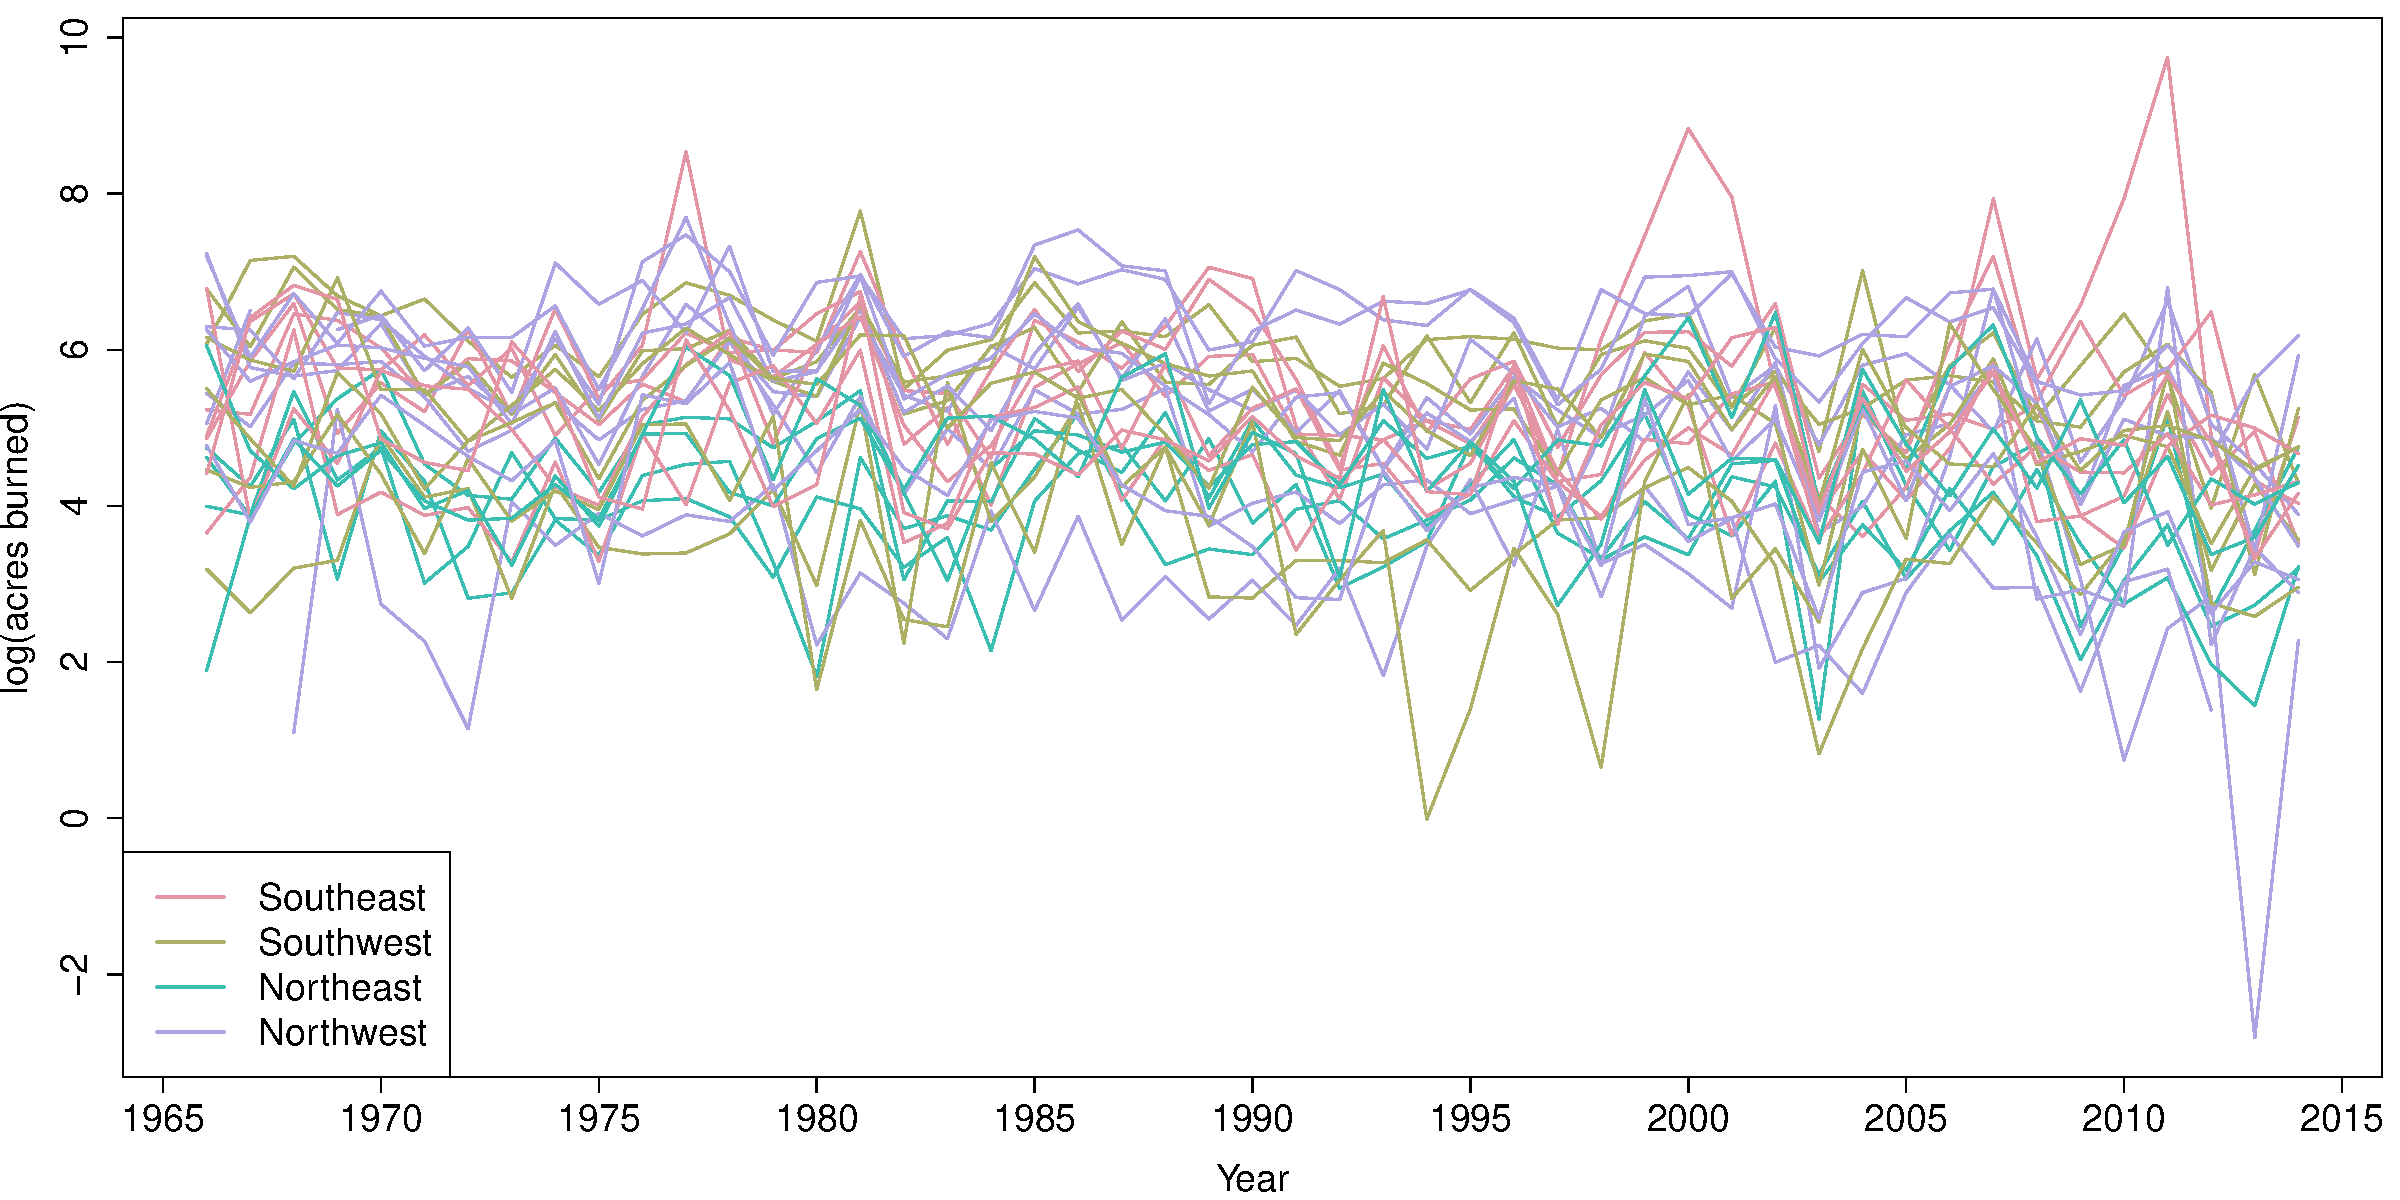
\includegraphics[width=0.55\linewidth]{plots/fire-spag-rand-25}
  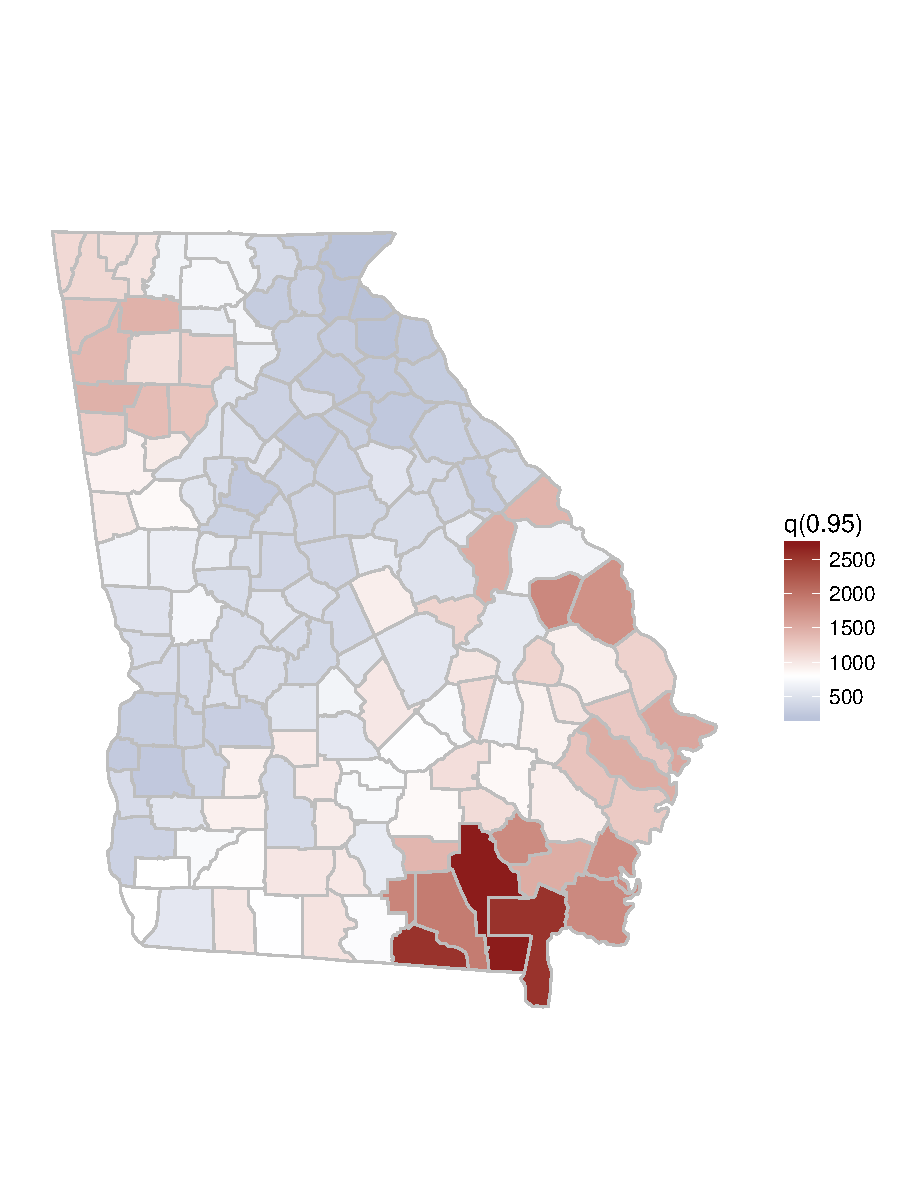
\includegraphics[width=0.44\linewidth, trim = 0 8em 0 10em]{plots/fire-spatial-q95.pdf}
  \caption{Time series of log acres burned for 25 randomly selected counties with colors coding the county's quadrant (left), and spatially smoothed threshold values, $T_i$ for each county (right).}
  \label{ebfig:firets25}
\end{figure}

We estimate the extremal coefficient function $\hat{\theta}_{ij}$ by setting $q_1 = 0.90$ and using $n_q = 100$.
With more data, it would possible to increase $q_1$, but we set $q_1 = 0.90$ to increase the stability when estimating $\hat{\vartheta}_{ij}$.
Because these data are not block-maxima, we select a site-specific threshold $T_i$ to use in the analysis with the following algorithm.
Without some adjustment to the data, it is challenging to borrow information across sites to inform the threshold selection.
We first standardize the data, separately by county, by subtracting the site's median and dividing by the site's interquartile range.
Denote the standardized data by $\widetilde{\bY}_i$.
% \begin{align}
%   \widetilde{\bY}_i = \frac{\bY_i - \text{med}(\bY_i)}{\text{IQR}(\bY_i)}
% \end{align}
% where med$(\cdot)$ is the median, and IQR$(\cdot)$ is the inter-quartile range.
Then we combine all sites together and plot a mean residual plot for $\widetilde{Y}_{it}, i = 1, \ldots, n_s$ and $t = 1, \ldots, n_t$.
The mean residual plot is given in \fref{ebfig:mrlthresh}.
Based upon the mean residual plot, we select the 95th percentile for the threshold.
To calculate $T_i$ for each county, we use the 95th percentile for the combined data for county $i$ and its five closest counties (see \fref{ebfig:firets25}).

\begin{figure}[htbp]  % markdown/eda/eda-plotting.R
  \centering
  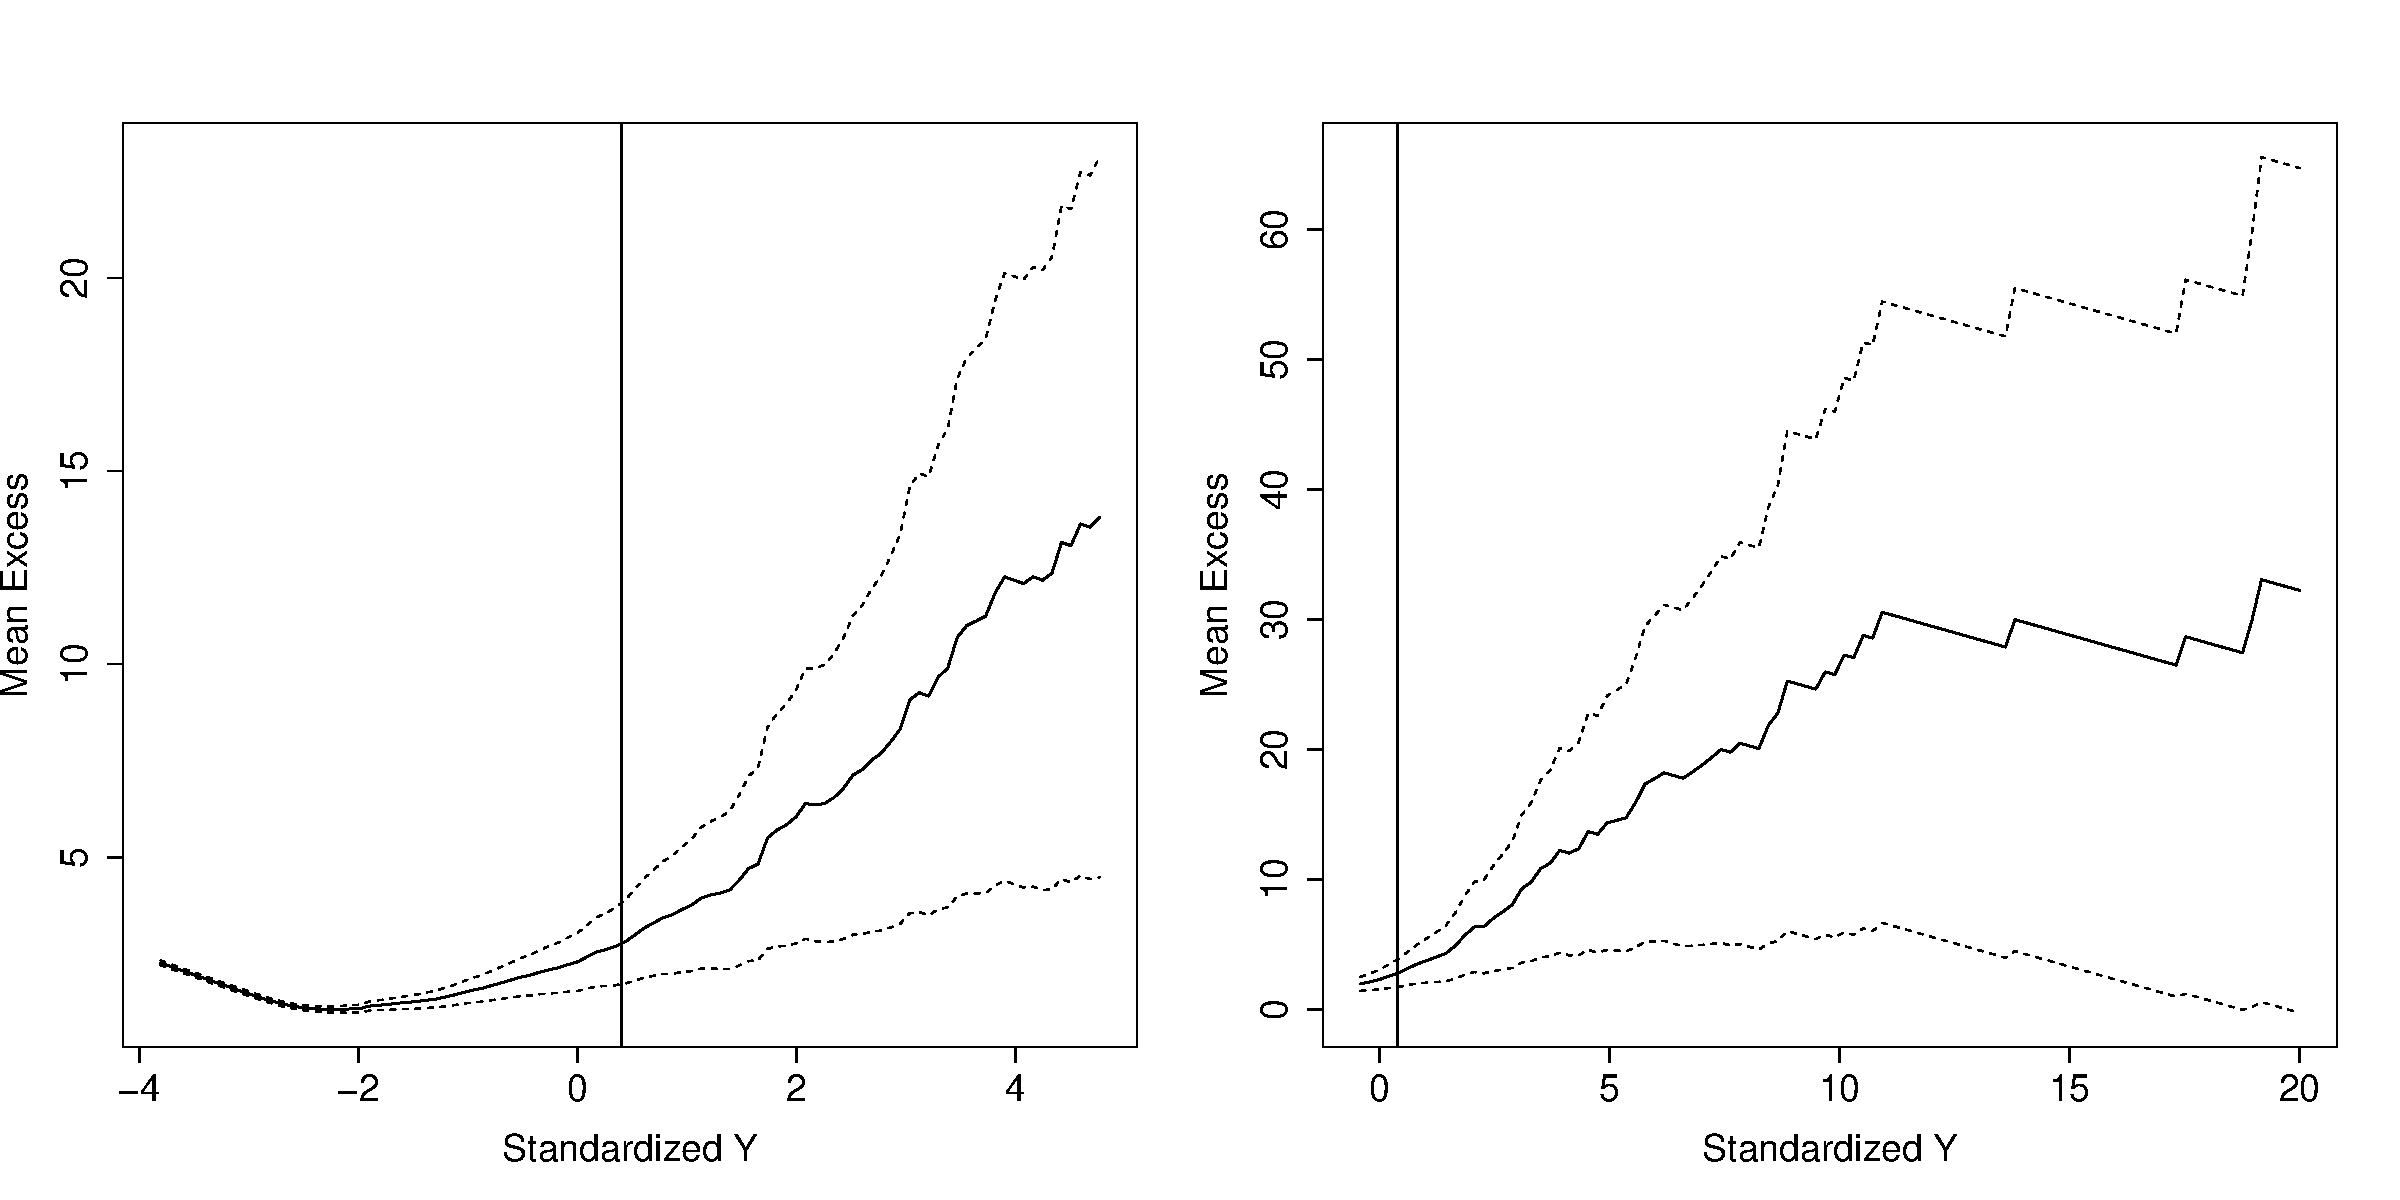
\includegraphics[width = \linewidth]{plots/fire-mrl-plots.pdf}
  \caption{Mean residual plot for the data pooled across counties after standardizing using the county's median and interquartile range. The two panels show different ranges on the x-axis and include a vertical line at the sample 95th percentile.}
  \label{ebfig:mrlthresh}
\end{figure}

%\begin{figure}[htbp]
%  \centering
%  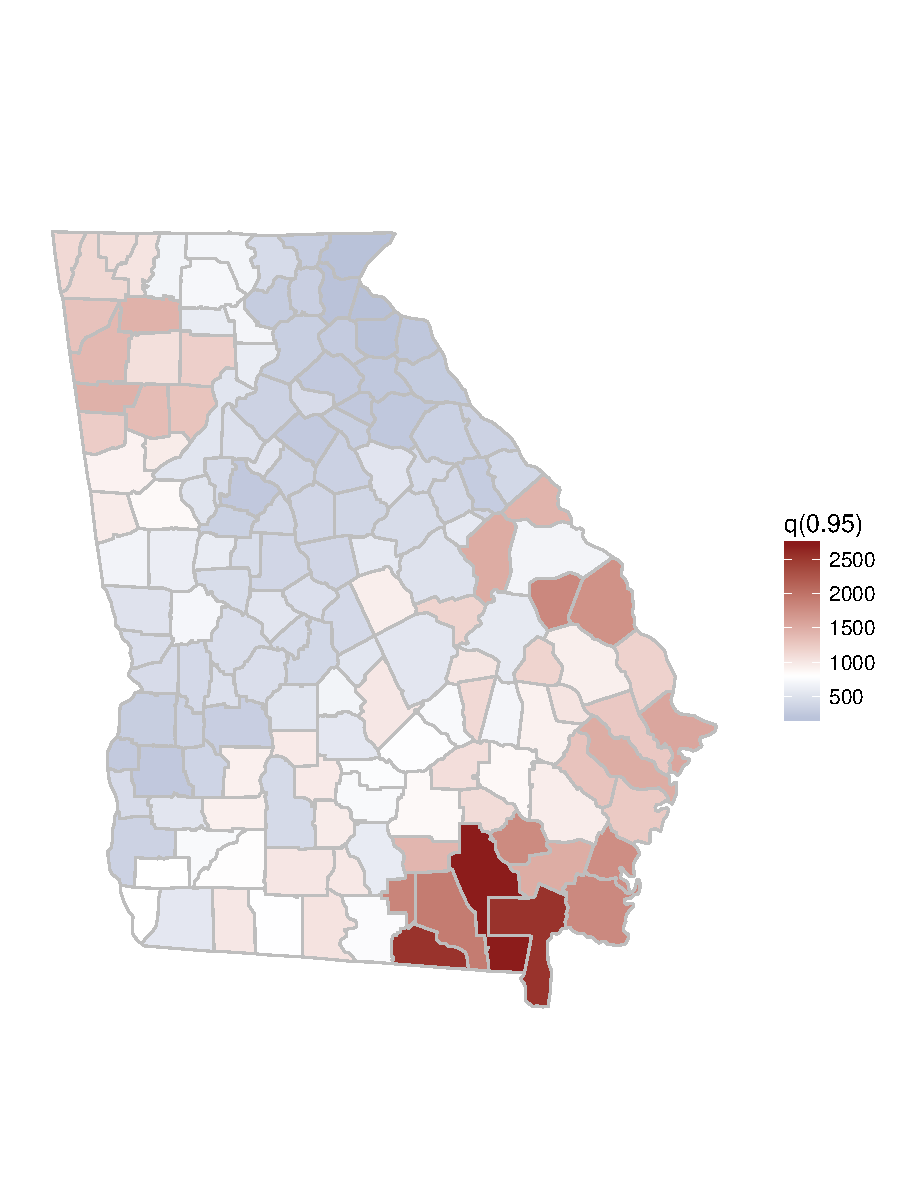
\includegraphics[width = 0.47\linewidth, trim = 0 10em 0 10em]{plots/fire-spatial-q95.pdf}
%  \caption{Spatially smoothed threshold values for each county.}
%  \label{fig:mrlthresh}
%\end{figure}

The empirical basis functions for the analysis can be used to help explore spatial dependence in the extremes.
The first six EBFs for the wildfire data along with the cumulative sum of the contributions for $v_1, \ldots, v_{25}$ are given in \fref{ebfig:fire-ebfpanel}.
\begin{figure}[htbp] % markdown/fire-analysis/basis-functions.R
  \centering
  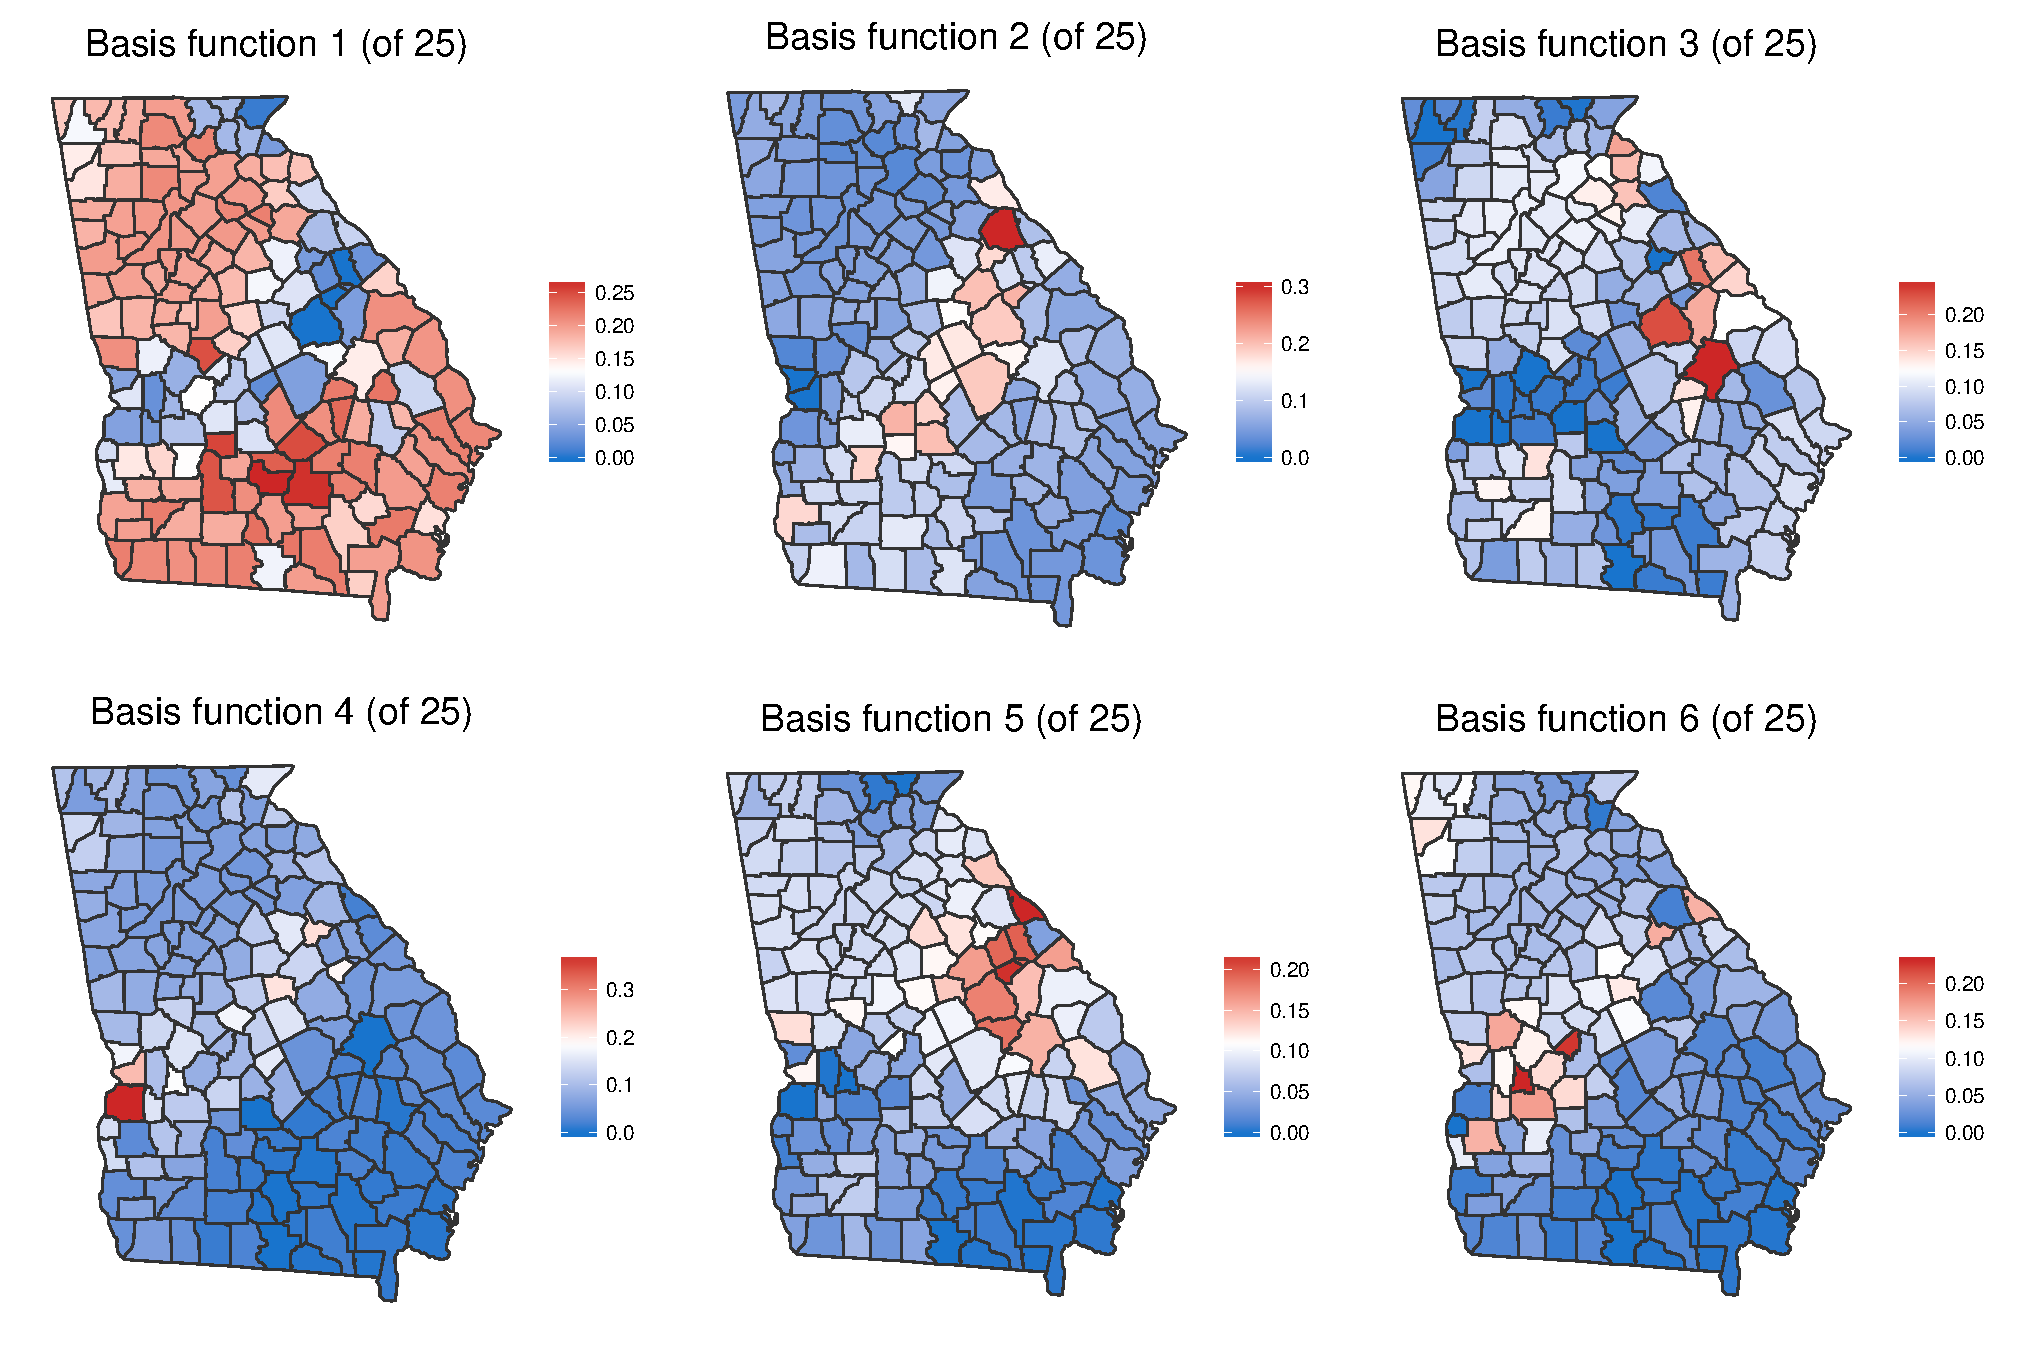
\includegraphics[width=\linewidth]{plots/fire-ebf-panel.pdf}\\
  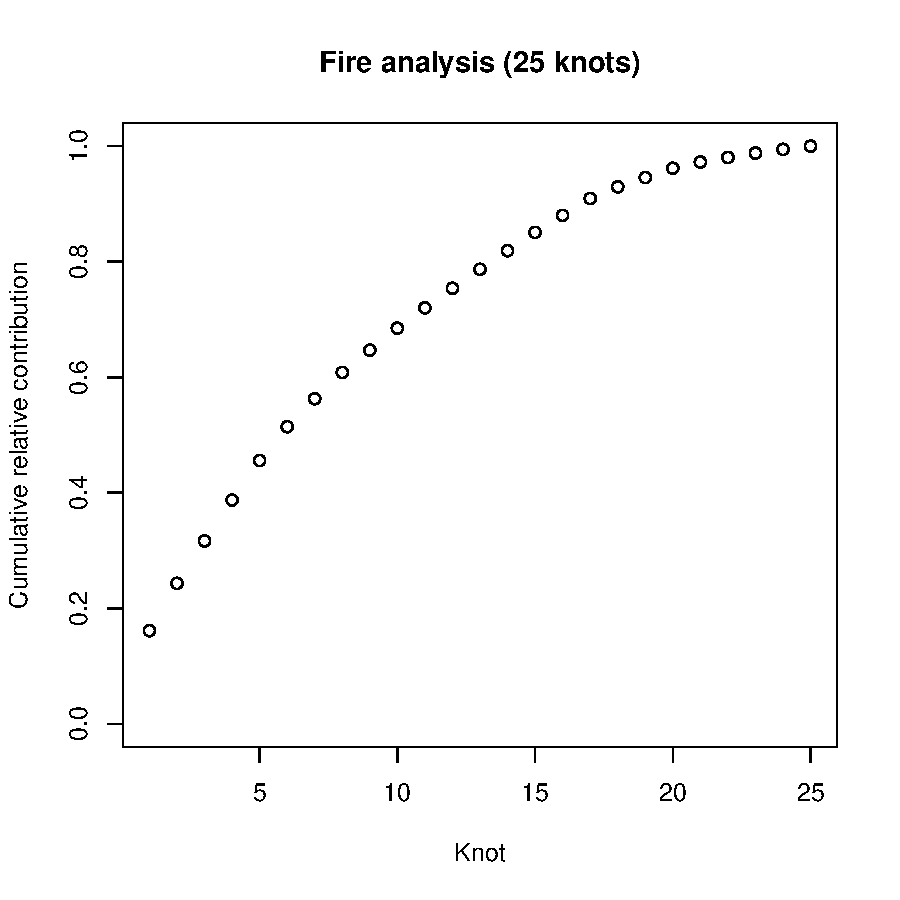
\includegraphics[width=0.45\linewidth]{plots/firev-25.pdf}
  \caption{First six EBFs for the Georgia fire data and the cumulative sum of contributions $v_1, \ldots, v_{25}$.}
  \label{ebfig:fire-ebfpanel}
\end{figure}
The first EBF roughly separates the Southeastern Plains (blue) from the coastal region in the southeast and mountains regions in the northeast (red).
The remaining EBFs further partition the plains.
As a comparison, we provide the first six principal components of the fire data along with the cumulative sum of the first 25 eigenvalues in \aref{eba:pca}.

Given the basis function estimates, we run the MCMC for 35,000 iterations using a burnin period of 25,000 iterations.
We consider models fit with both EBF and GSK, and fit the model using $L = 5, 10, \ldots, 40$.
Timing for each setting of $L$ for 1,000 iterations is given in \tref{ebtbl:fire-scores}.
These timings come from a single core of an Intel Core i7-5820K Haswell-E processor, using the OpenBLAS optimized BLAS library (\url{http://www.openblas.net}).

\subsection{Results for fire analysis}\label{ebs:results-fire}
We use 10-fold cross-validation to assess the predictive performance of a model.
For each method, we randomly select 90\% of the observations across counties and years to be used as a training set to fit the model.
The remaining 10\% of sites and years are withheld for testing model predictions.
To assess the predictions for the test set, we use quantile scores and Brier scores \citep{Gneiting2007}.
The quantile score (QS) for quantile level $q^*$ is given by \mbox{$2 \{I[Y(\bs) > \hat{q}(\bs)] - q^*]\}\{\hat{q}(\bs) - Y(\bs)\}$} where $\hat{q}(\bs)$ is the estimated $q^*$th quantile at site $\bs$, and $I[\cdot]$ is an indicator function.
The Brier score (BS) for predicting an exceedance of a level $c$ at site $\bs$ is given by \mbox{$\{I[Y(\bs) > c] - \hat{P}[Y(\bs) > c]\}^2$}.
For both of these methods, a lower score indicates a better fit.
The Brier and quantile scores for the fire analysis are given in \tref{ebtbl:fire-scores}. %, and a plot of the scores are given in \fref{ebfig:fire-bsqs}.
For the data, the BS and QS are fairly similar for all number of basis functions and the EBF versus GSK.
This is perhaps due to the spatial variation in the marginal distribution explaining most of the spatial variation.
In fact, using the EBFs, the estimate of residual dependence for the fire data is $\hat{\alpha} = 0.861$ ($\alpha = 1$ is residual independence).

\begin{table}[htbp]
\caption{Average Brier scores ($\times 100$), average quantile scores for $q(0.95)$ and $q(0.99)$, and time (in minutes) for 1,000 iterations for fire analysis.}
\label{ebtbl:fire-scores}
\centering
  \begin{tabular}{llcrrcrrcc}
  \toprule
  & & \phantom{ab} & \multicolumn{2}{c}{Brier Scores ($\times 100$)} & \phantom{abc} & \multicolumn{2}{c}{Quantile Scores} & \phantom{ab} & \\
  \cmidrule{4-5} \cmidrule{7-8}
  & Process && $q(0.95)$ & $q(0.99)$ && $q(0.95)$ & $q(0.99)$ && Time\\
  \midrule
  L = 5  & EBF && 4.269 & 1.653 && 107.904 & 67.345 && 1.16\\
         & GSK && 4.244 & 1.644 && 103.822 & 64.046 && 1.18\\
  \midrule
  L = 10 & EBF && 4.328 & 1.675 && 107.075 & 66.300 && 1.56\\
         & GSK && 4.170 & 1.665 && 104.214 & 64.589 && 1.47\\
  \midrule
  L = 15 & EBF && 4.330 & 1.690 && 108.381 & 67.671 && 1.86\\
         & GSK && 4.214 & 1.654 && 104.490 & 65.201 && 1.83\\
  \midrule
  L = 20 & EBF && 4.346 & 1.697 && 107.389 & 66.957 && 2.18\\
         & GSK && 4.174 & 1.646 && 104.671 & 65.430 && 2.20\\
  \midrule
  L = 25 & EBF && 4.263 & 1.650 && 106.656 & 64.913 && 2.54\\
         & GSK && 4.216 & 1.661 && 104.208 & 64.468 && 2.55\\
  \midrule
  L = 30 & EBF && 4.328 & 1.678 && 106.265 & 64.674 && 2.90\\
         & GSK && 4.228 & 1.660 && 104.143 & 64.443 && 2.92\\
  \midrule
  L = 35 & EBF && 4.329 & 1.671 && 106.817 & 65.002 && 3.29\\
         & GSK && 4.256 & 1.663 && 105.016 & 64.920 && 3.32\\
  \midrule
  L = 40 & EBF && 4.284 & 1.653 && 106.621 & 64.753 && 3.70\\
         & GSK && 4.233 & 1.666 && 105.301 & 64.932 && 3.56\\
  \bottomrule
  \end{tabular}
\end{table}

% \begin{figure}[htbp]  % markdown/fire-analysis/combine-tables.R
%   \centering
%   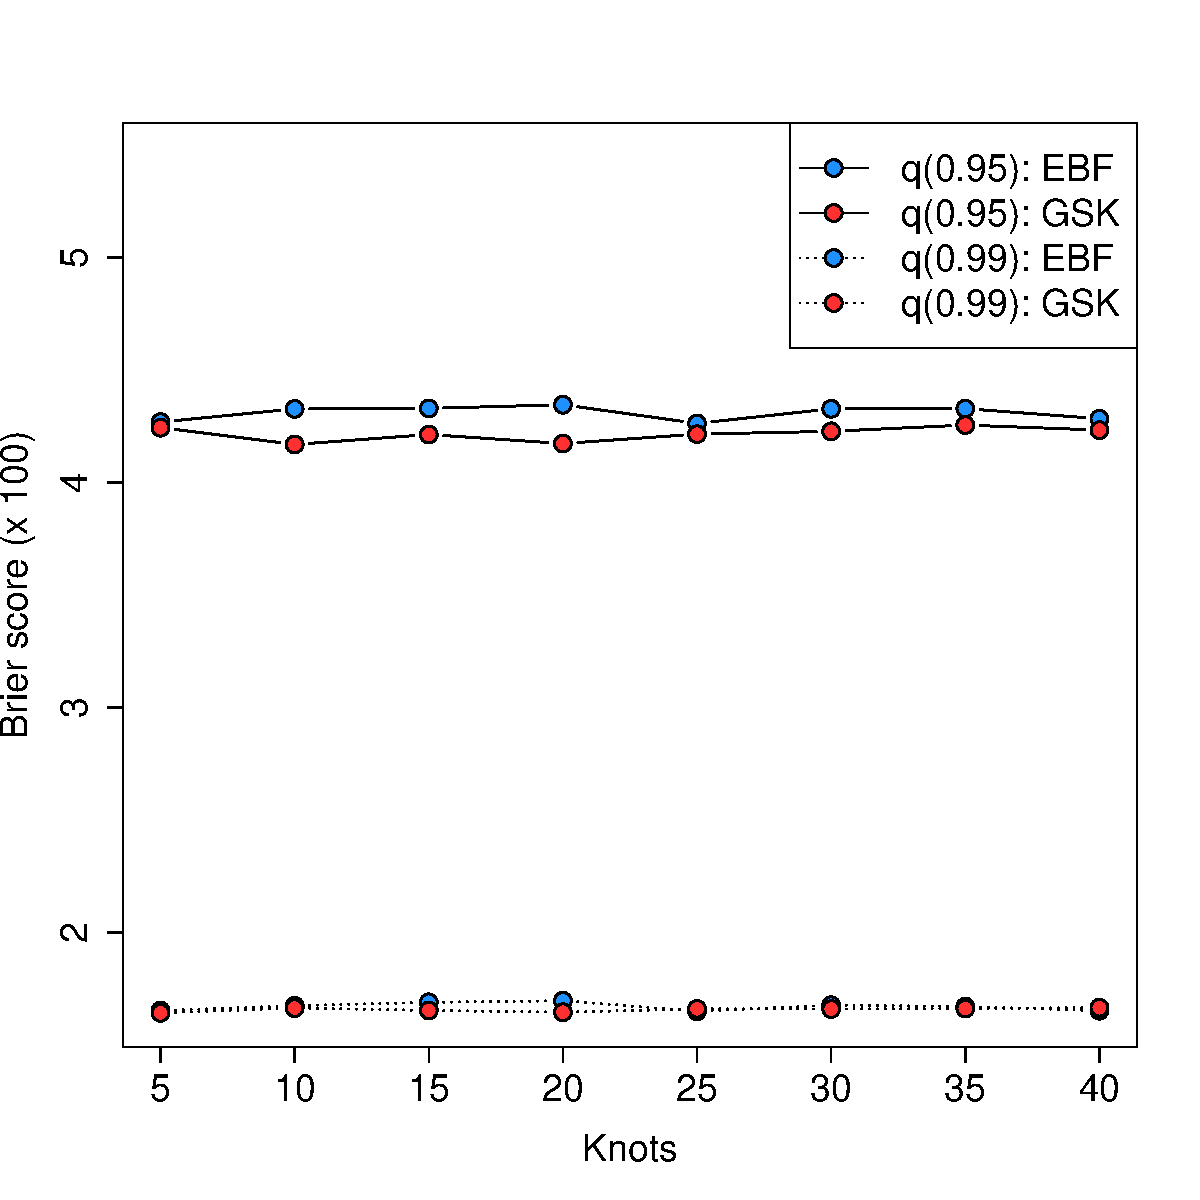
\includegraphics[width=0.49\linewidth]{plots/fire-bs.pdf}
%   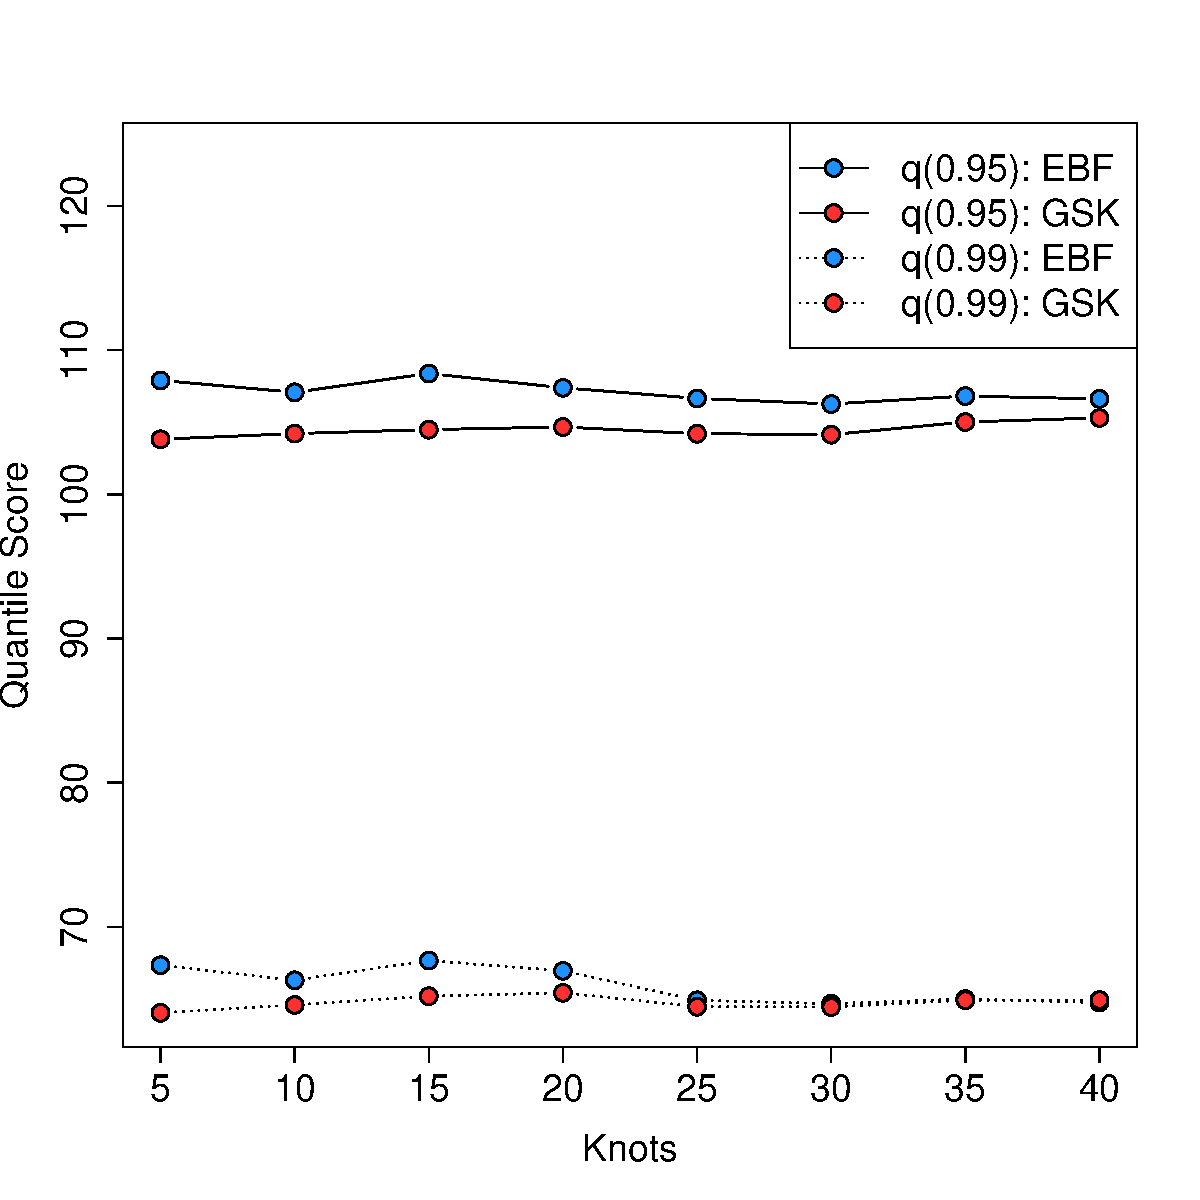
\includegraphics[width=0.49\linewidth]{plots/fire-qs.pdf}
%   \caption{Brier scores (left) and quantile scores (right) for $q(0.95)$ and $q(0.99)$ to compare EBF and GSK analysis of Georgia fire data.}
%   \label{ebfig:fire-bsqs}
% \end{figure}

% \begin{figure}[htbp]  % markdown/fire-analysis/posterior_map.R
%   \centering
%   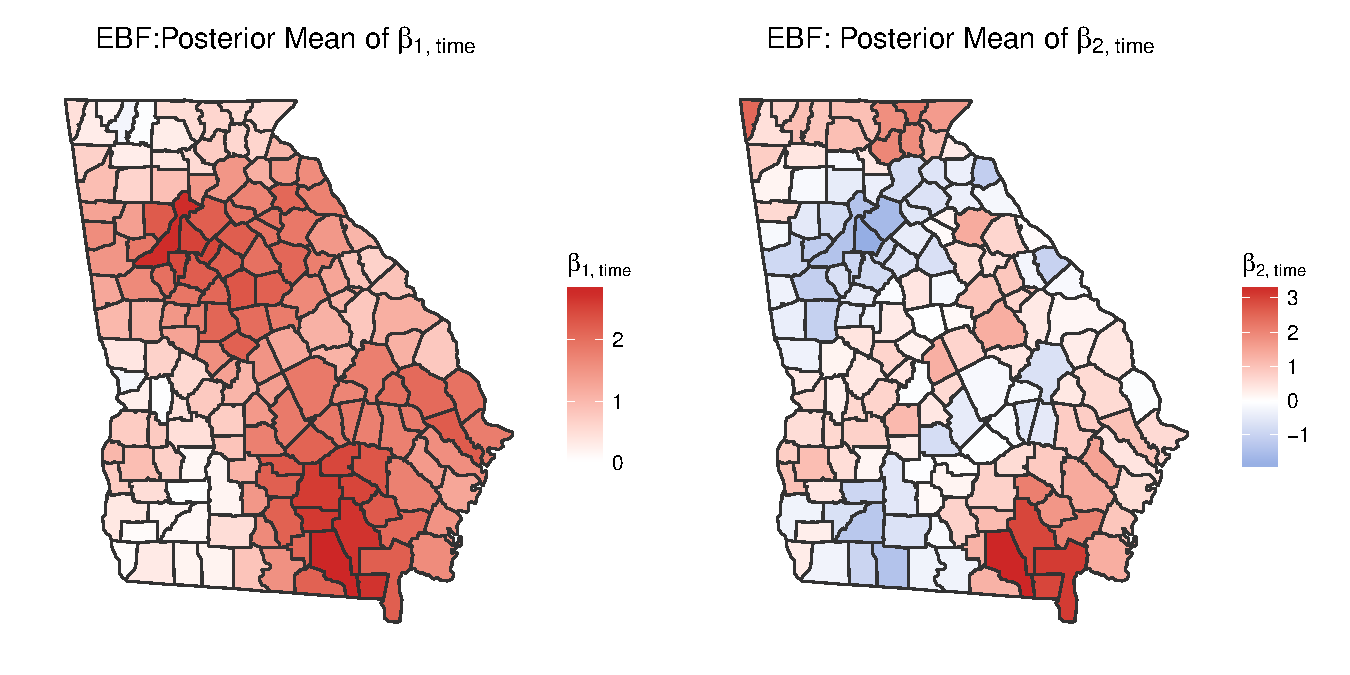
\includegraphics[width=\linewidth]{plots/fire-ebf-post-betatime.pdf}
%   \caption{Posterior mean of $\beta_{1, \text{time}}$ (left) and $\beta_{2, \text{time}}$ (right) for fire data using EBF.}
%   \label{ebfig:fire-ebfpostbeta1}
% \end{figure}

% \begin{figure}[htbp]  % markdown/fire-analysis/posterior_map.R
%   \centering
%   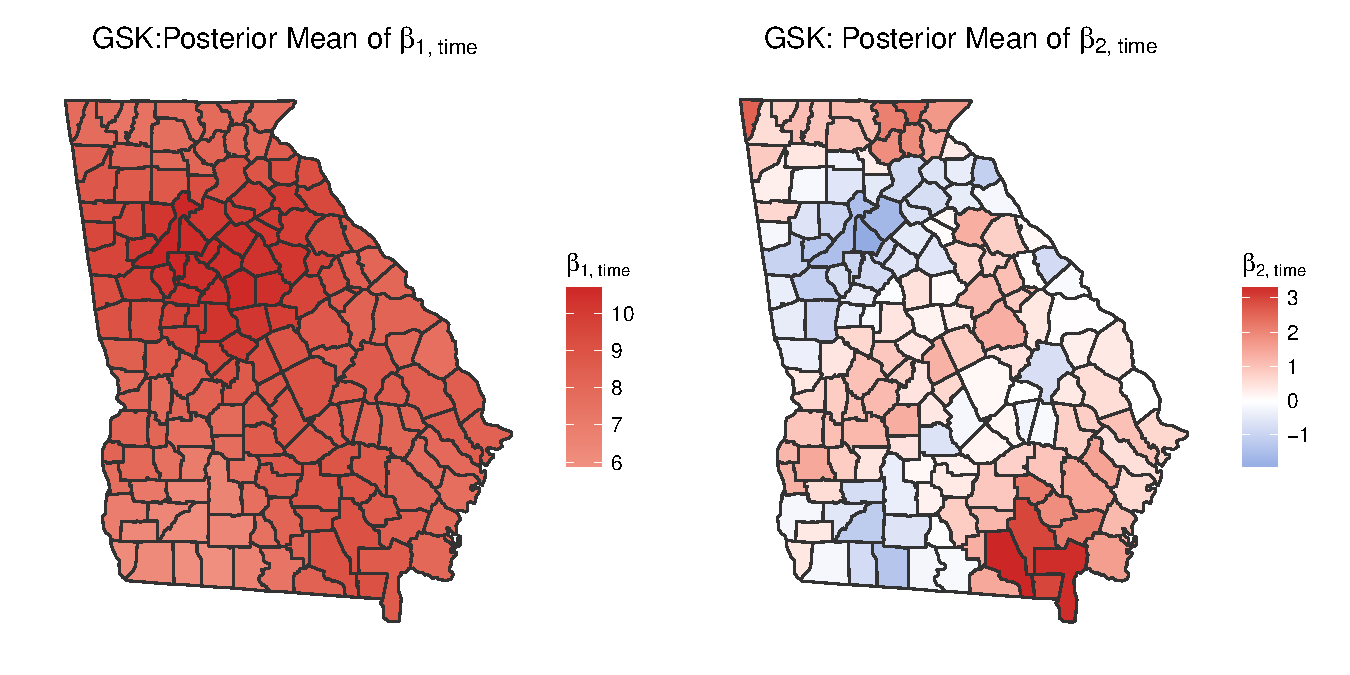
\includegraphics[width=\linewidth]{plots/fire-gsk-post-betatime.pdf}
%   \caption{Posterior mean of $\beta_{1, \text{time}}$ (left) and $\beta_{2, \text{time}}$ (right) for fire data using GSK.}
%   \label{ebfig:fire-gskpostbeta1}
% \end{figure}

% \begin{figure}[htbp]  % markdown/fire-analysis/posterior_map.R
%   \centering
%   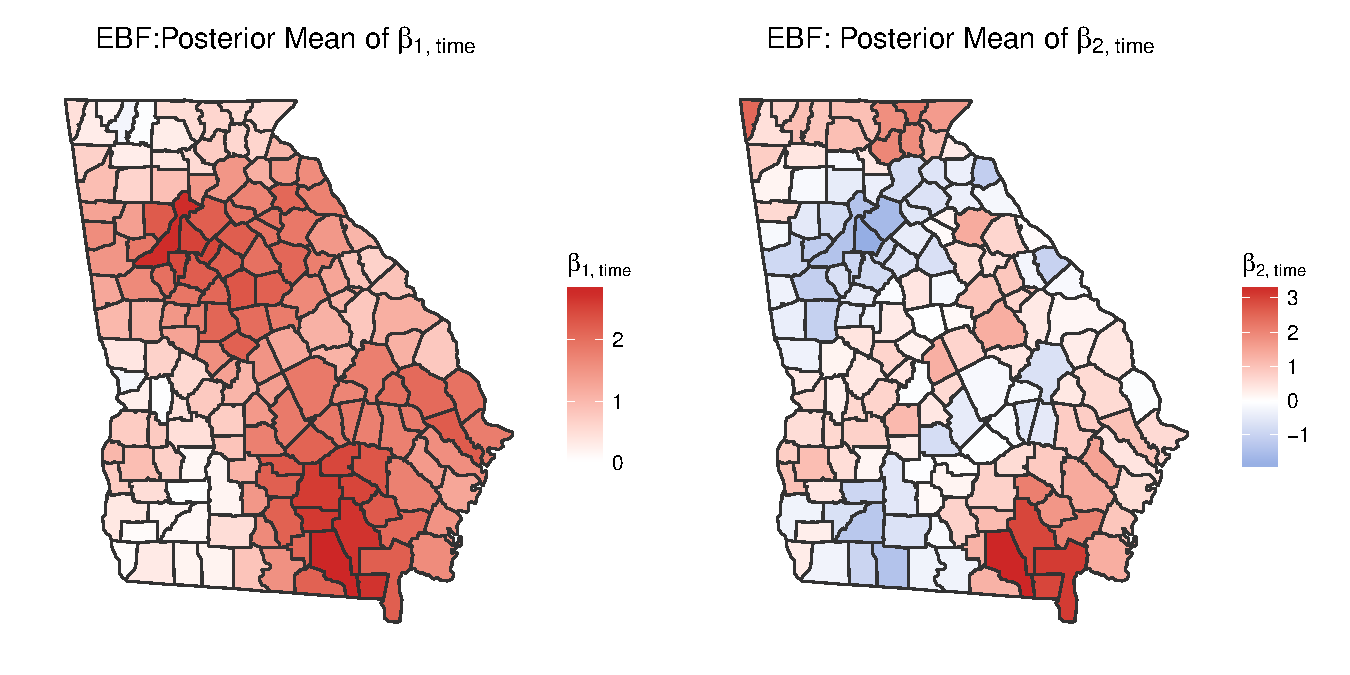
\includegraphics[width=\linewidth]{plots/fire-ebf-post-betatimepos.pdf}
%   \caption{Posterior P$(\beta_{1, \text{time}} > 0)$ (left) and P$(\beta_{2, \text{time}} > 0)$ (right) for fire data using EBF.}
%   \label{ebfig:fire-ebfpostbeta1pos}
% \end{figure}

% \begin{figure}[htbp]  % markdown/fire-analysis/posterior_map.R
%   \centering
%   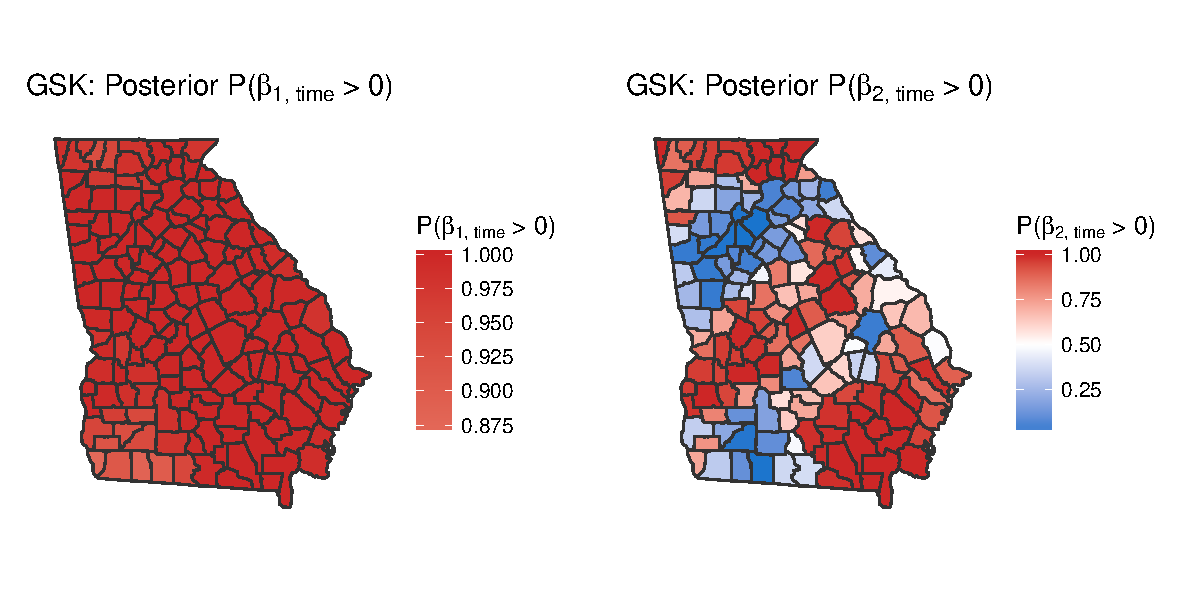
\includegraphics[width=\linewidth]{plots/fire-gsk-post-betatimepos.pdf}
%   \caption{Posterior P$(\beta_{1, \text{time}} > 0)$ (left) and P$(\beta_{2, \text{time}} > 0)$ (right) for fire data using GSK.}
%   \label{ebfig:fire-gskpostbeta1pos}
% \end{figure}

Based on the cross-validation results, we run a full analysis using all of the data with $L = 25$.
Despite the GSK model having slightly smaller BS and QS values, we use the EBF method.
\fref{ebfig:fire-ebf-postpanel} gives posterior summaries for three quantities of interest.
We provide maps of the linear time trend in the GEV location ($\beta_{1, \text{time}, i}$), and GEV log scale  ($\beta_{2, \text{time}, i}$)  and a map of \mbox{$\Delta Q90_i = Q90_{i, 2014} - Q90_{i, 1965}$} the change in the mean of the posterior distribution of $Q90_{i, t}$ between $t_1 = 1965$ and $t_2 = 2014$.
We also provide maps of the posterior probability that each of the three terms is positive.

We construct the posterior distribution of the the estimated 90th quantile $Q90_{i, t}$ using the GEV parameters as follows.
Let $Q90_{i, t}^{(j)}$ be the estimated 90th quantile at site $i$ for time $t$ at iteration $j$.
We first compute
\begin{align}
  \mu_{i, t}^{(j)} &= \beta_{1, \text{int}, i}^{(j)} + \beta_{1, \text{time}, i}^{(j)} t \\
  \log\left(\sigma_{i, t}^{(j)}\right) &= \beta_{2, \text{int}, i}^{(j)} + \beta_{2, \text{time}, i}^{(j)} t. \nonumber
\end{align}
Let $Q90_{i, t}^{(j)} = \mu_{i, t}^{(j)} + \sigma_{i, t}^{(j)} F^{-1}\left(0.90, \xi^{(j)}\right)$ where $F^{-1}(q, \xi)$ is the inverse distribution function of the GEV$(1, 1, \xi)$ distribution evaluated at the $q$th quantile.
Finally, let $Q90_{i, t}$ be posterior mean of $Q90_{i, t}^{(j)}$.
To obtain the posterior probability of seeing an increase over time, we take the posterior distributions of each parameter of interest at the two time points.
Consider two time points $t_1 < t_2$.
Let $\varphi_t^{(j)}$ be the parameter of interest at iteration $j$ and time $t$.
We then take the posterior mean of $I\left[\varphi_{t_2}^{(j)} > \varphi_{t_1}^{(j)}\right]$, for the posterior probability of seeing an increase in $\varphi$ from time $t_1$ to $t_2$.

These results suggest that there has been a slight increase in the amount of acres burned over time.
When looking at the variability of the acres burned over time, we see some patterns that generally correspond to landcover in Georgia (see \url{http://narsal.uga.edu/} for landcover maps).
In the high intensity urban areas (e.g. the Piedmont region) and croplands, we see a decrease in variability as well as very low P$[\Delta Q90 > 0]$.
However, in the more forested areas (e.g. Blue Ridge mountains, Okefenokee Swamp), we see increased variability over time as well as a high P$[\Delta Q90 > 0]$.
This suggests that the 10-year return level for wildfires in regions with larger tree cover is increasing over time which corresponds with increased drought and higher temperatures.

\begin{figure}[htbp]  % markdown/fire-analysis/posterior_map.R
  \centering
  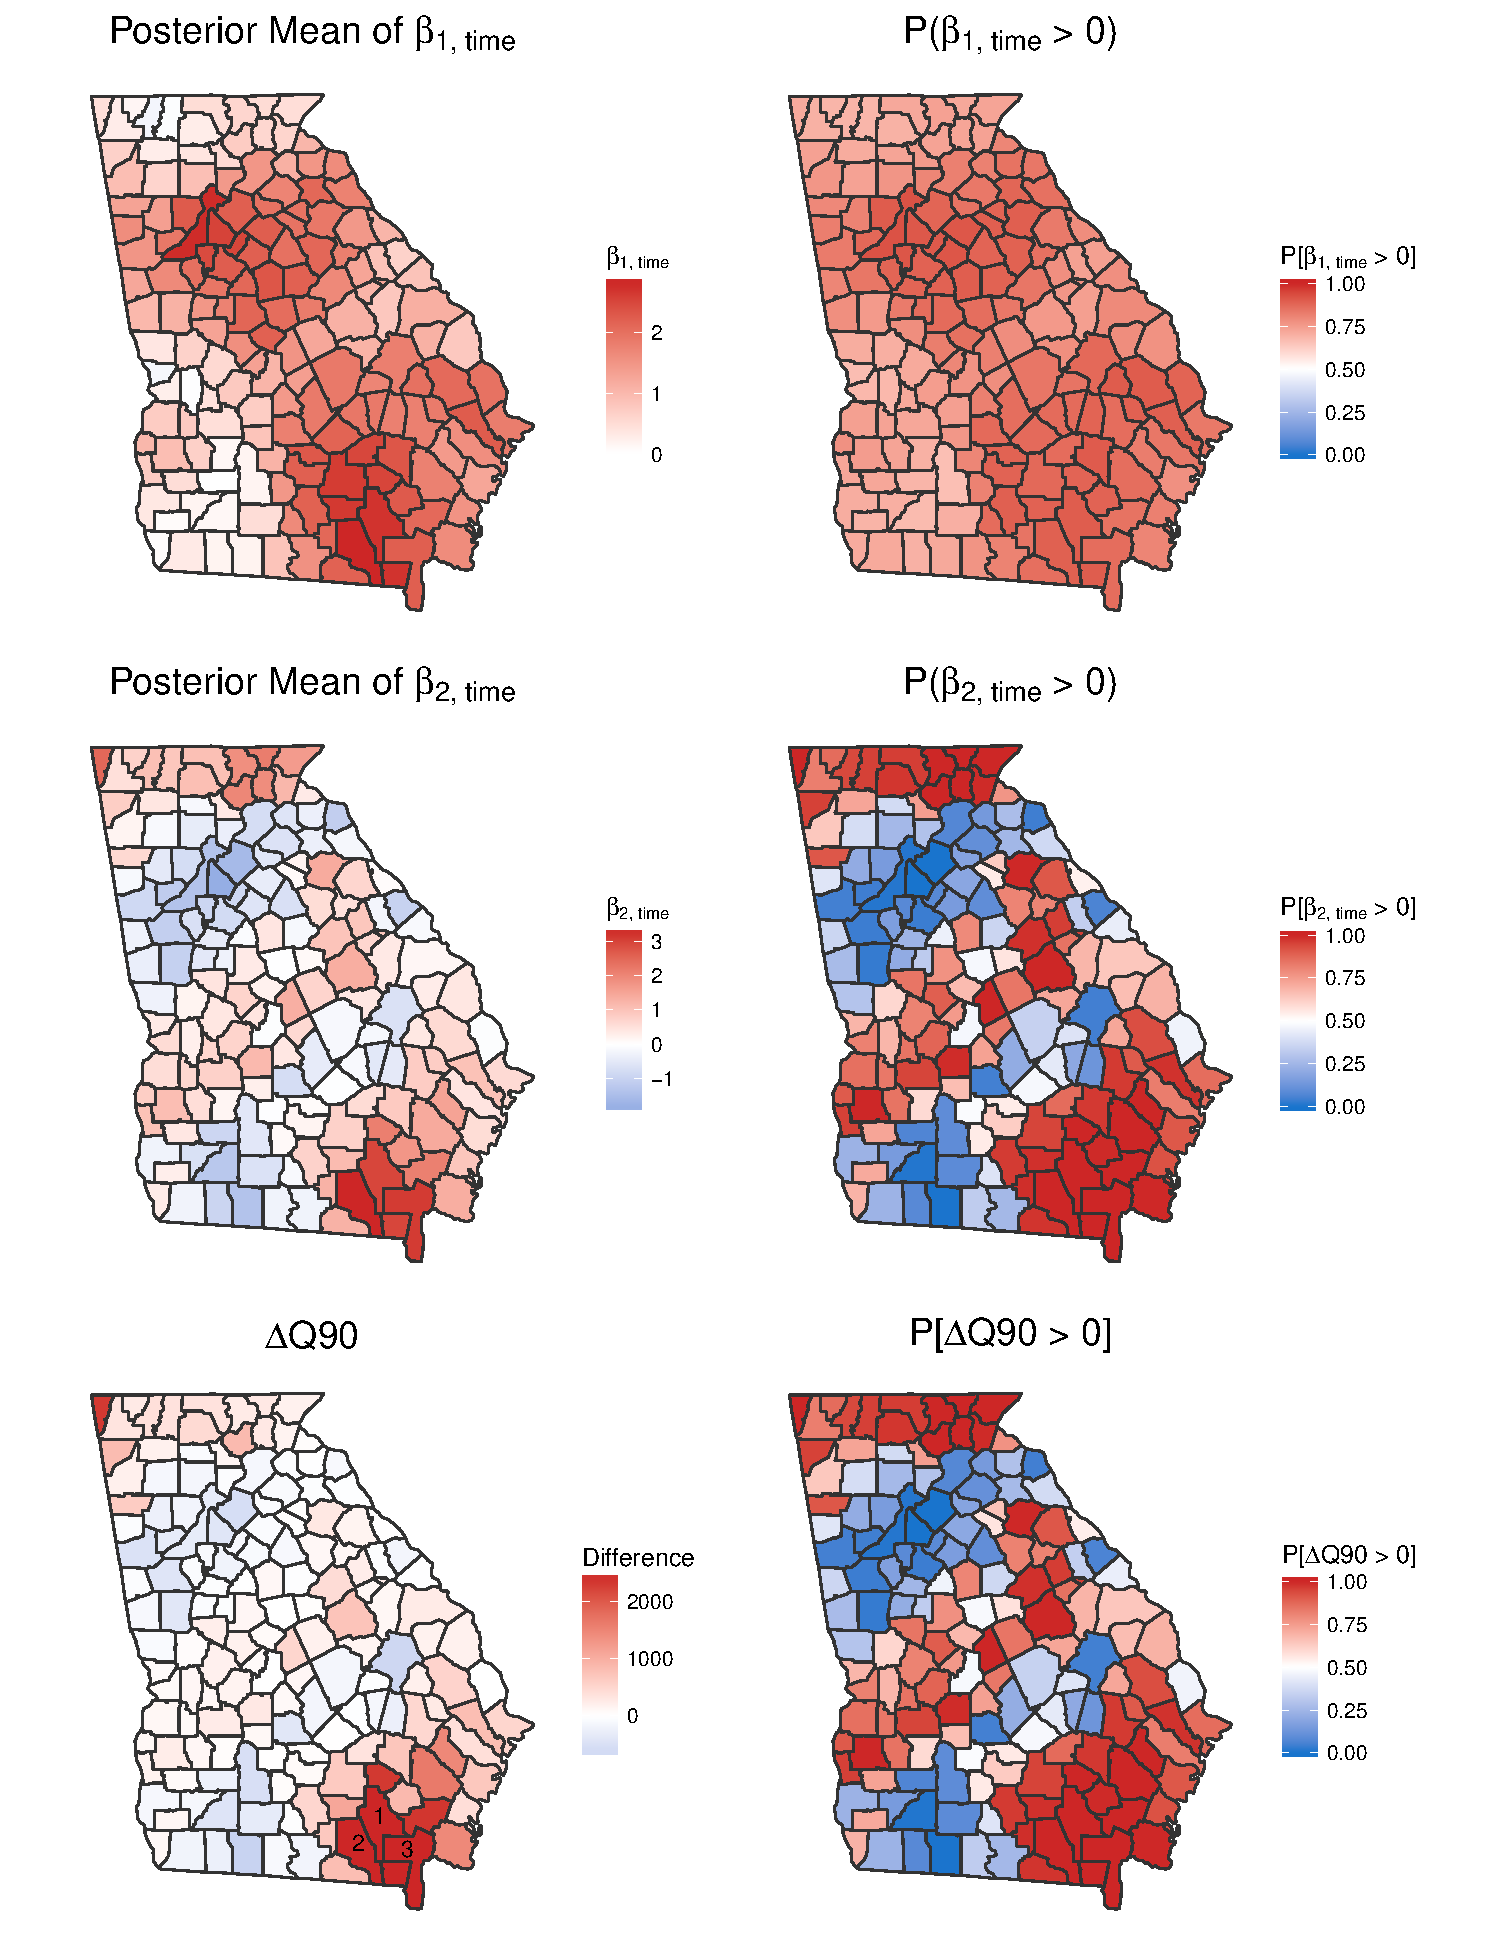
\includegraphics[height=0.9\textheight]{plots/fire-ebf-postpanel.pdf}
  \caption{Posterior mean of $\beta_{1, \text{time}}$ (top left), posterior mean of $\beta_{2, \text{time}}$ (middle left), estimate of $\Delta Q90$ (bottom left), P$[\beta_{1, \text{time}} > 0]$ (top right), P$[\beta_{2, \text{time}} > 0]$ (middle right), and P$[\Delta Q90 > 0]$ for fire data using EBF. In three counties (labeled), $\Delta Q90 > 2500$: County 1 - Ware (11,109), County 2 - Clinch (7,128), and County 3 - Charlton (6,545)}
  \label{ebfig:fire-ebf-postpanel}
\end{figure}

% \begin{figure}  % markdown/fire-analysis/combine-tables.R
%   \centering
%   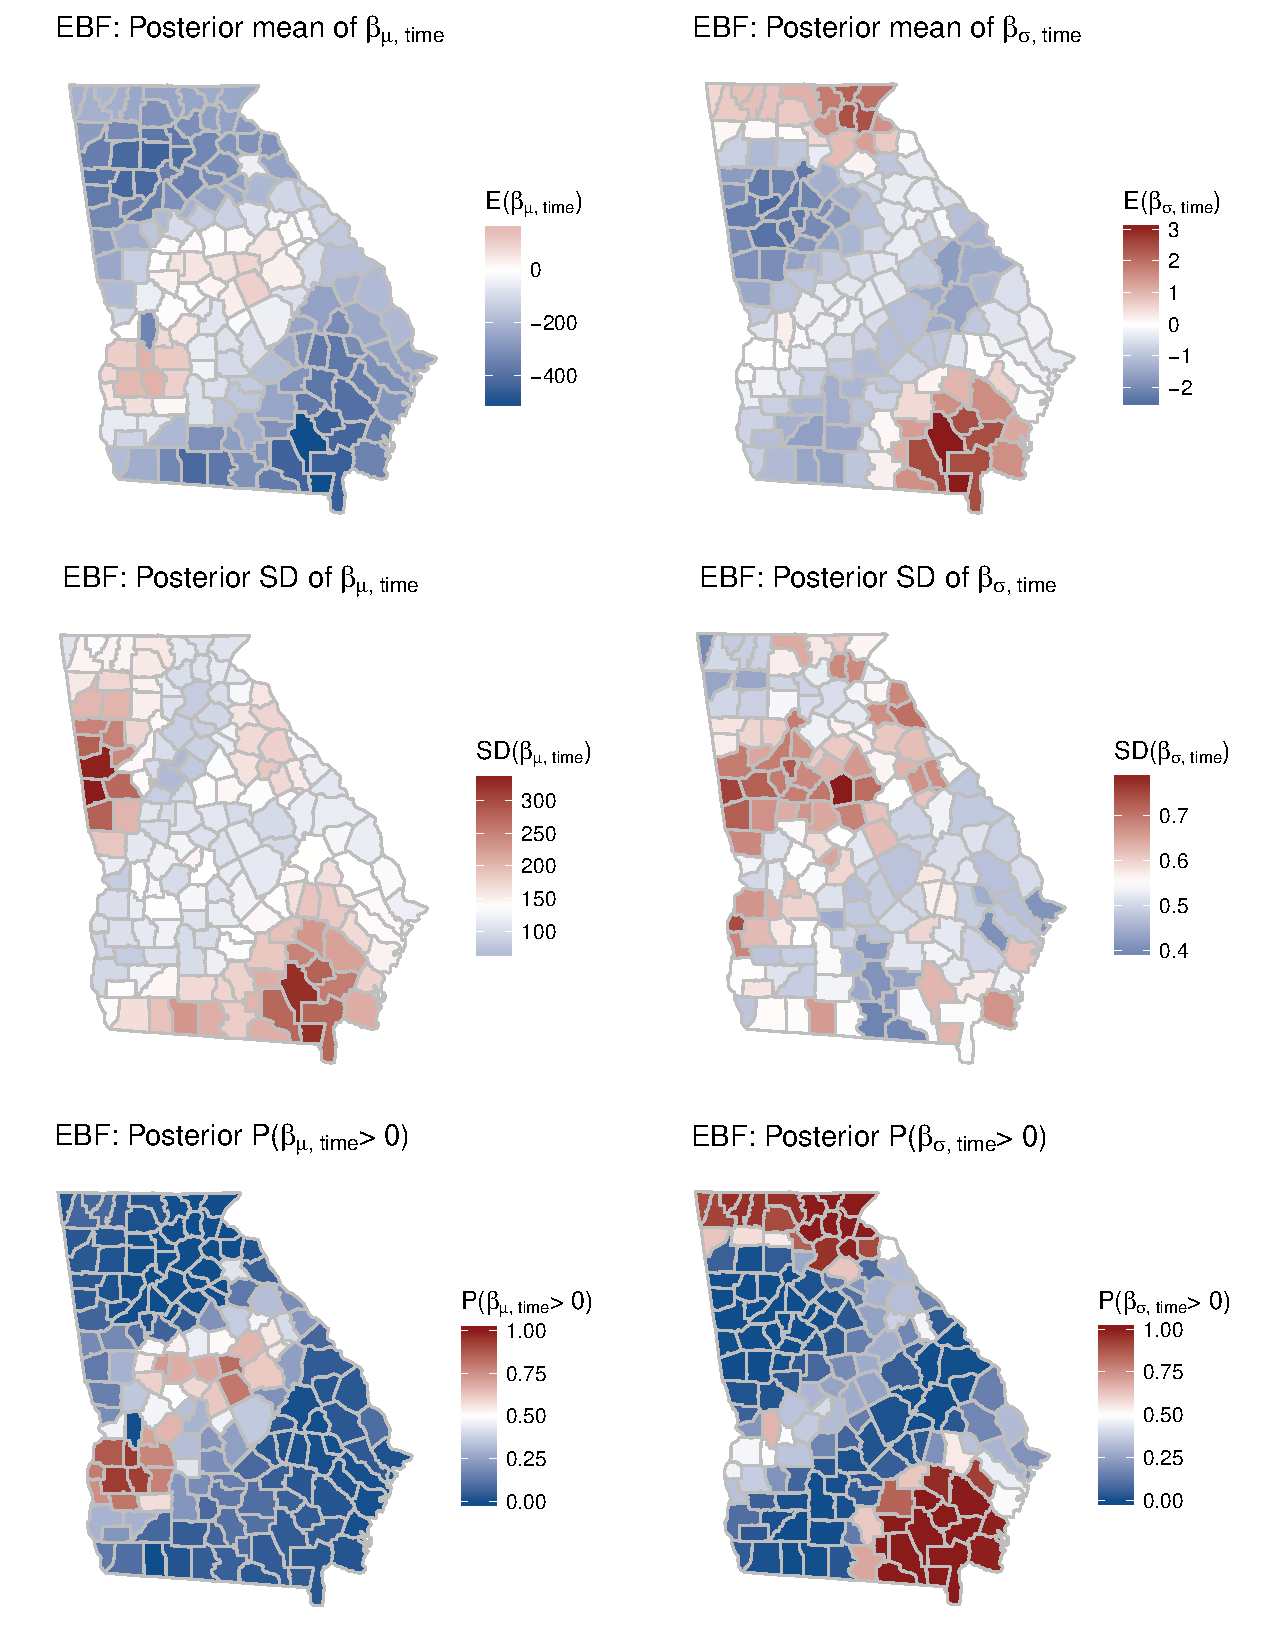
\includegraphics[width=\linewidth]{plots/ebf-post-betatime.pdf}
%   \caption{Posterior summaries of $\beta_{\text{time}}$ when using EBF for the spatial process with $L = 35$.}
%   \label{ebfig:ebfpost}
% \end{figure}

% \begin{figure}  % markdown/fire-analysis/combine-tables.R
%   \centering
%   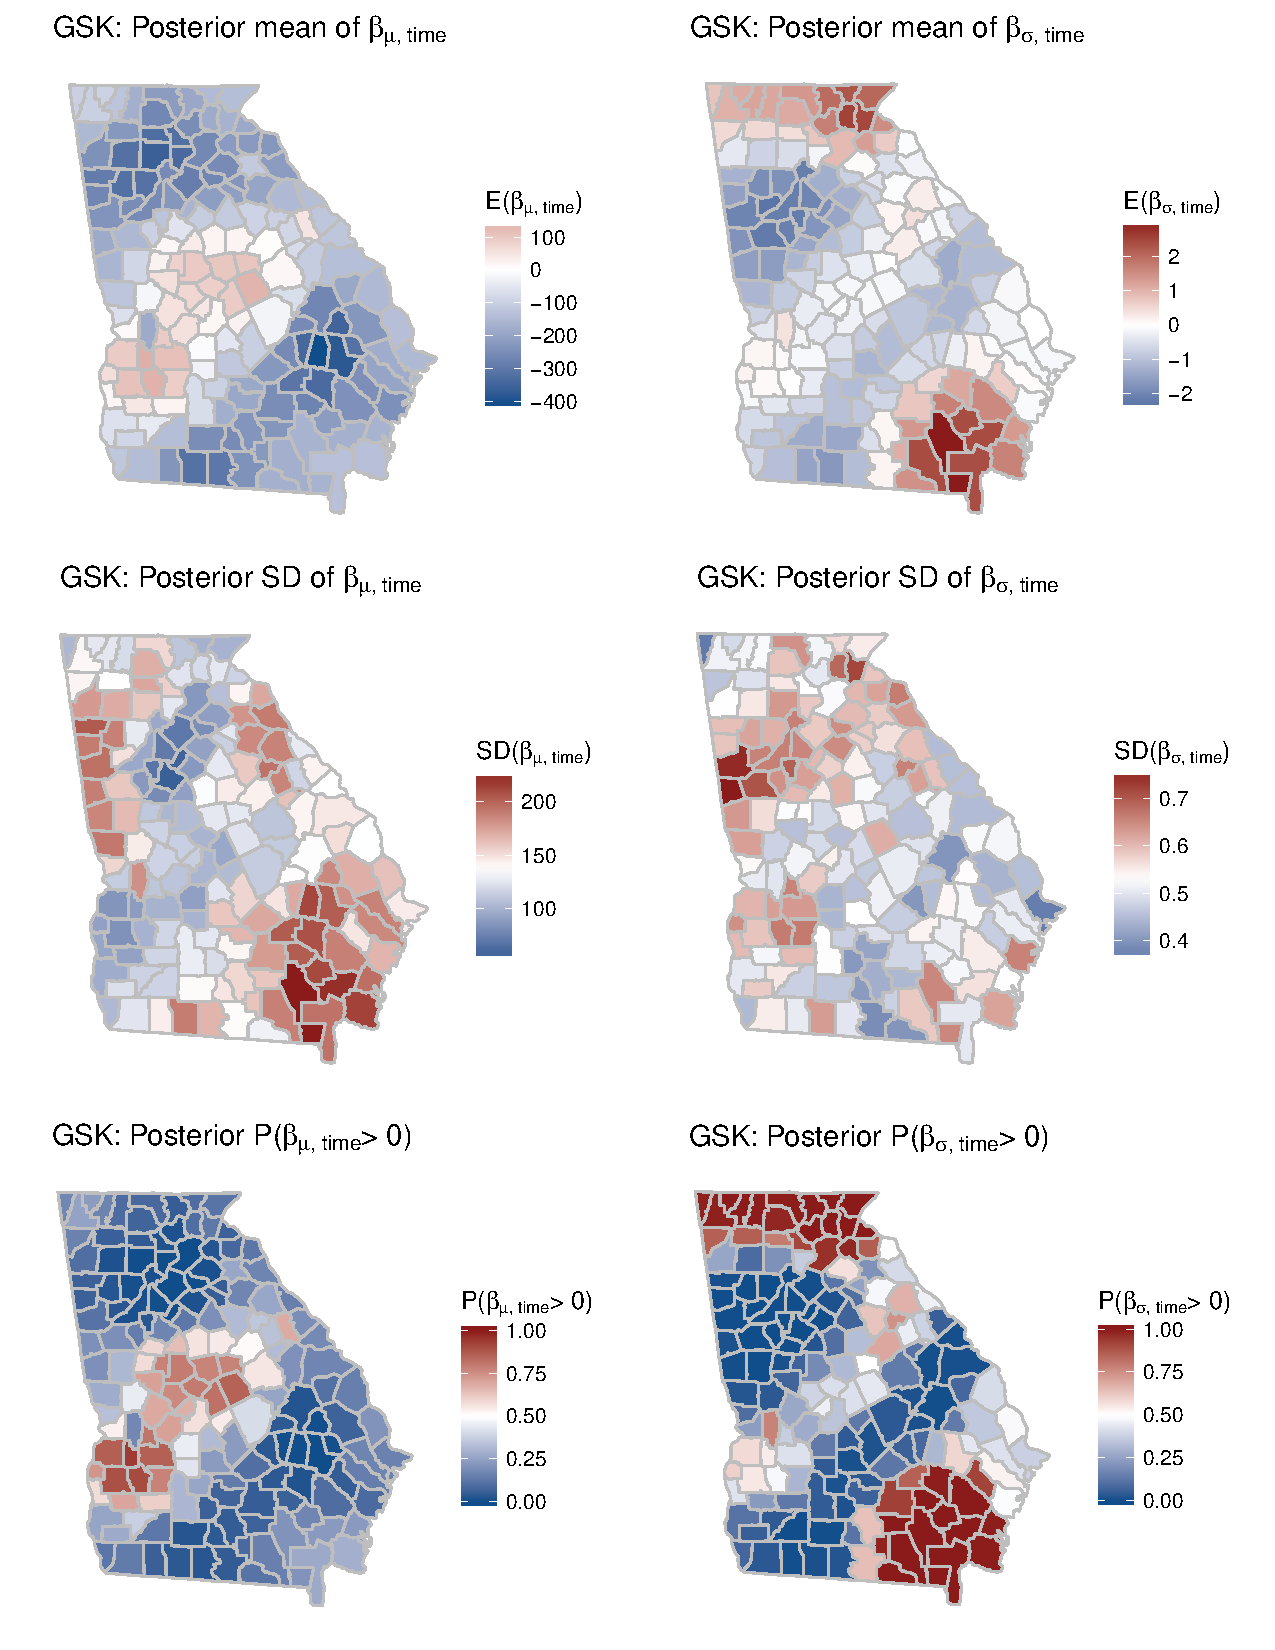
\includegraphics[width=\linewidth]{plots/gsk-post-betatime.pdf}
%   \caption{Posterior summaries of $\beta_{\text{time}}$ when using GSK for the spatial process with $L = 35$.}
%   \label{ebfig:gskpost}
% \end{figure}

% \begin{figure}  % markdown/fire-analysis/combine-tables.R
%   \centering
%   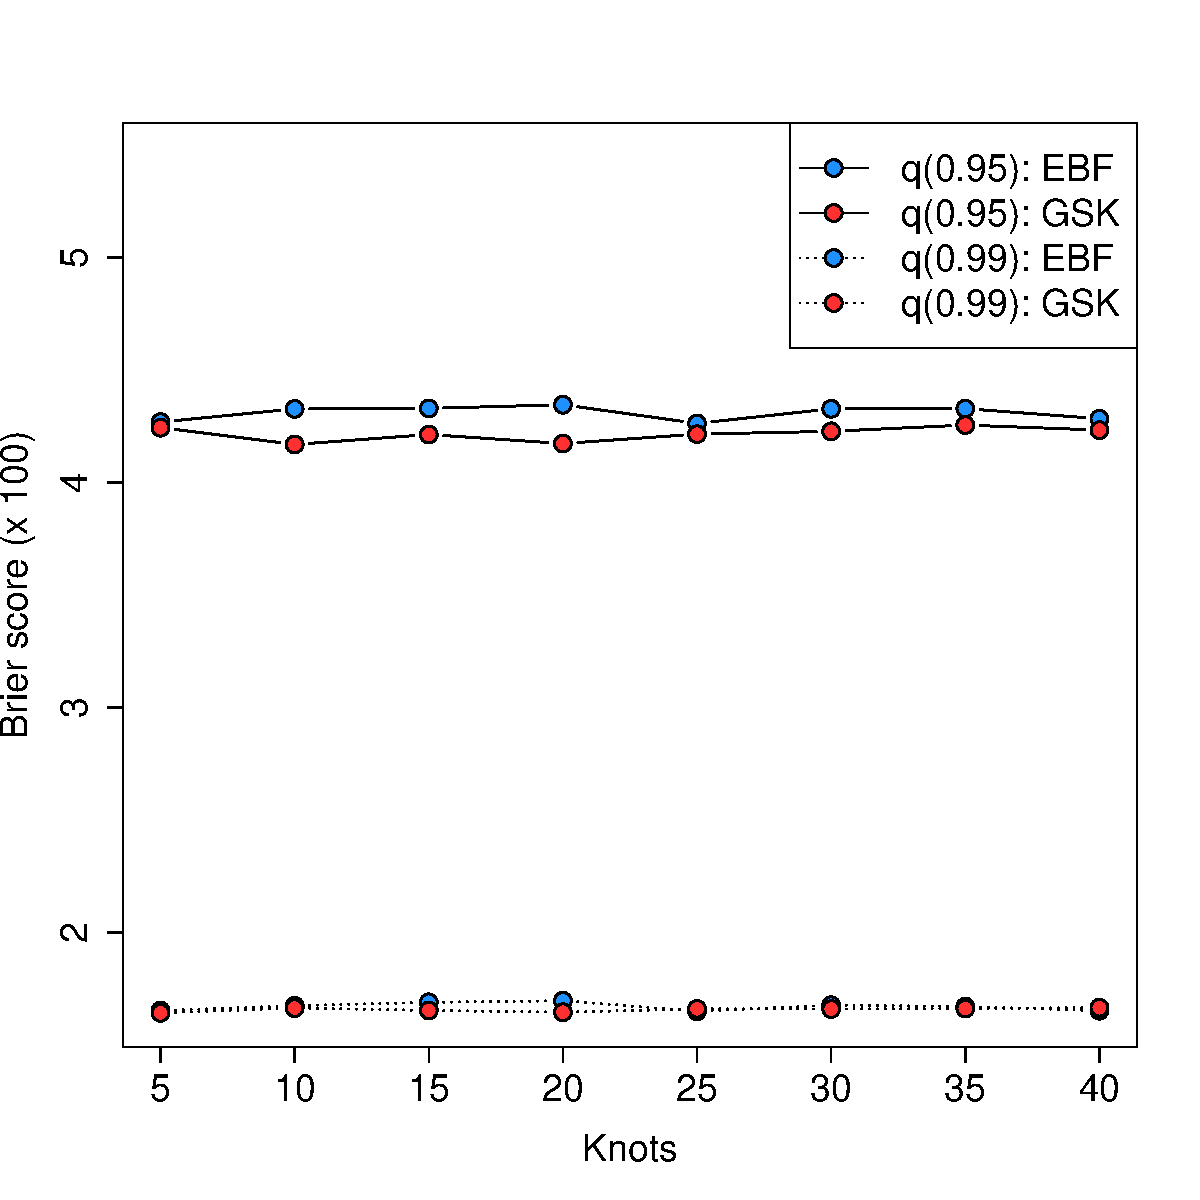
\includegraphics[width=0.47\linewidth]{plots/fire-bs}
%   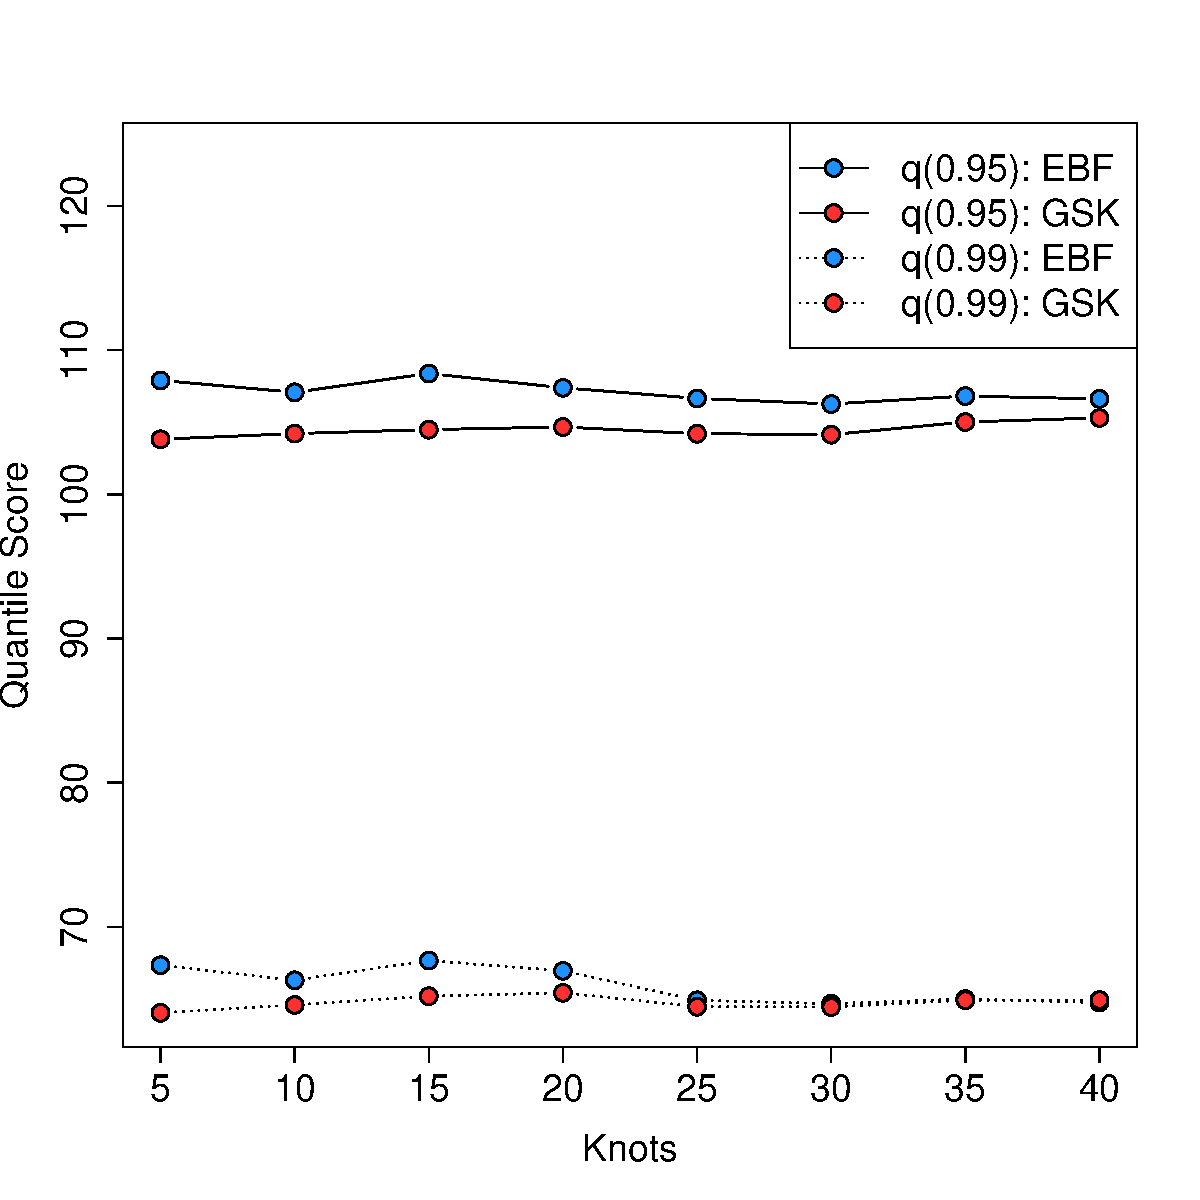
\includegraphics[width=0.47\linewidth]{plots/fire-qs}
%   \caption{Average Brier score for exceeding q(0.95) and q(0.99) (left). Average Quantile score for exceeding q(0.95) and q(0.99) (right).}
%   \label{fig:avgqscore}
% \end{figure}

% \begin{figure}  % markdown/fire-analysis/combine-tables.R
%   \centering
%   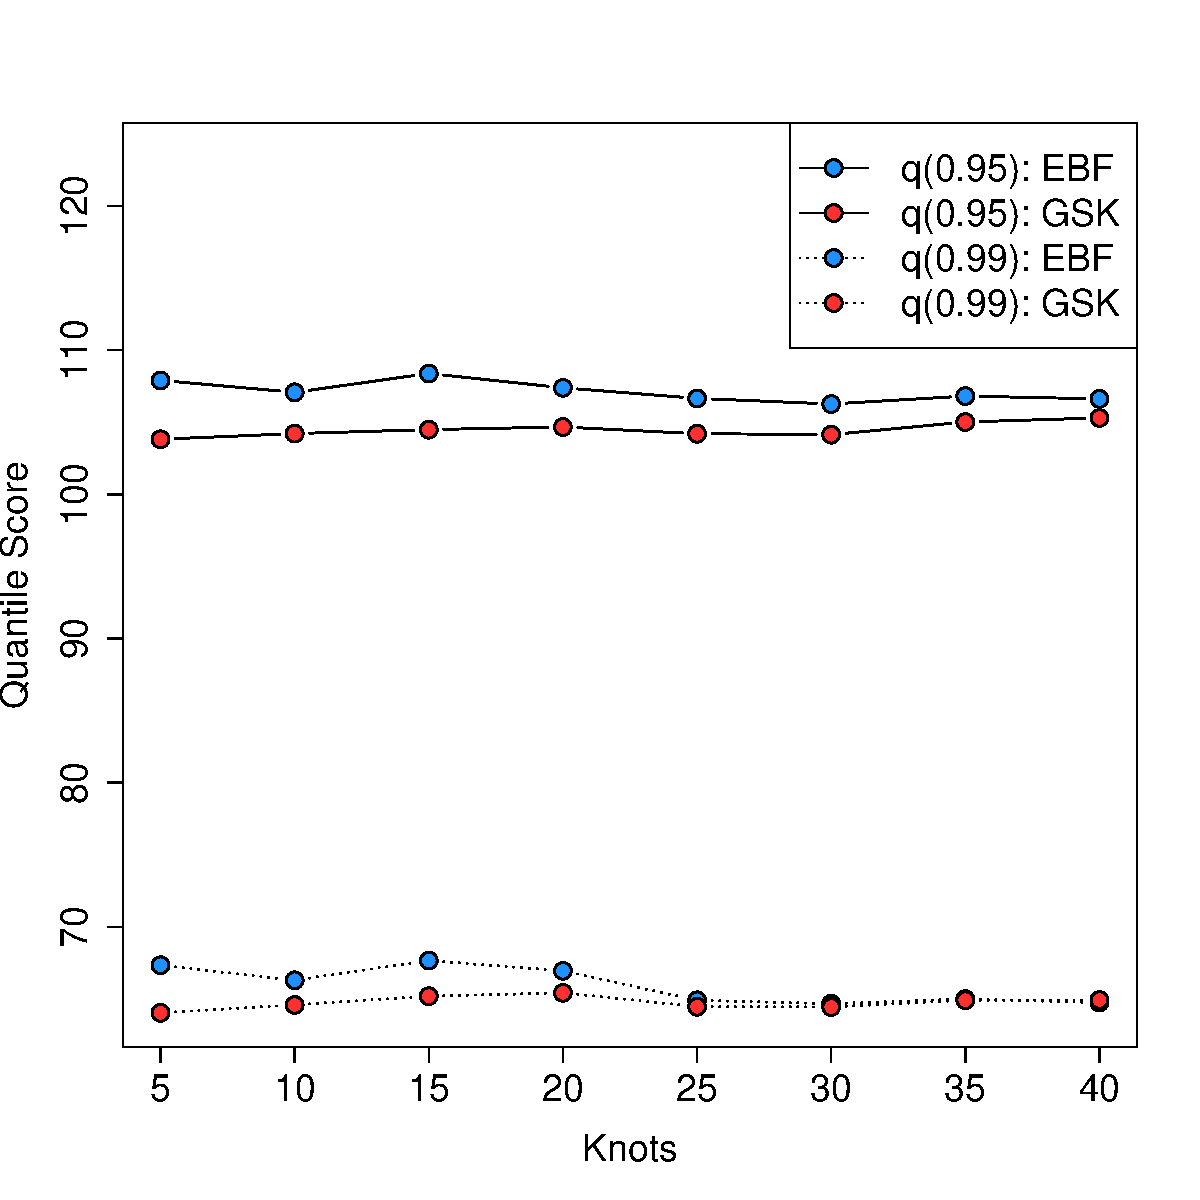
\includegraphics[width=\linewidth]{plots/fire-qs}
%   \caption{Average quantile score for q(0.95) (left). Average quantile score for q(0.99) (right).}
%   \label{fig:avgqscore}
% \end{figure}

% \begin{figure}  % markdown/fire-analysis/combine-tables.R
%   \centering
%   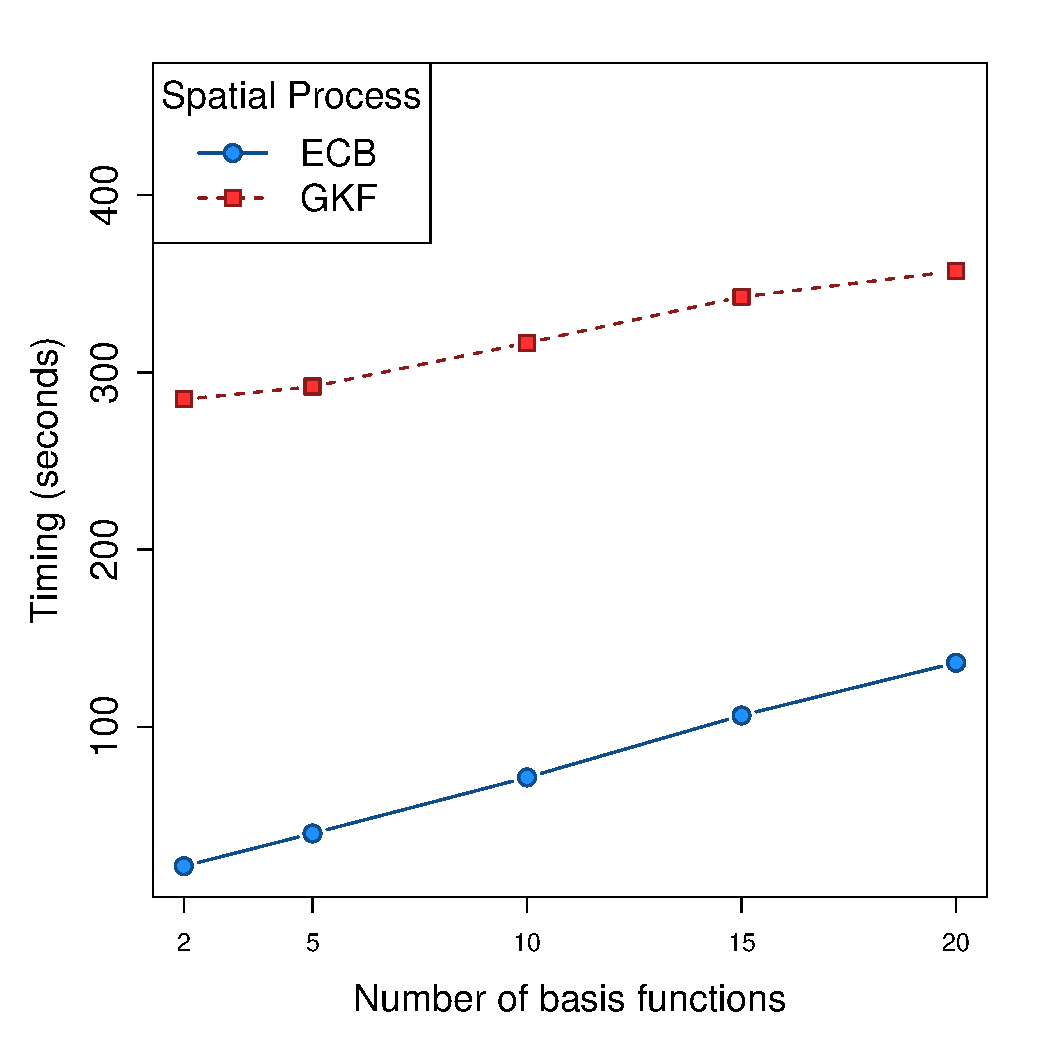
\includegraphics[width=0.47\linewidth]{plots/fire-timing}
%   \caption{Timing comparison of basis functions to kernel functions for the spatial process (100 iterations)}
%   \label{fig:timingcompare}
% \end{figure}

\subsection{Analysis of annual precipitation}\label{ebs:precip}
We also conduct an analysis of the precipitation data presented in \citet{Reich2012}.
The data are climate model output from the North American Regional Climate Change Assessment Program (NARCCAP).
This data consists of $n_s = 697$ grid cells at a 50km resolution in the eastern US, and includes historical data (1969 -- 2000) as well as future conditions (2039 -- 2070).
Because the data are block maxima, we set $T = -\infty$.

\begin{figure}[htbp]  % markdown/precipitation/cv-setup.R
  \centering
  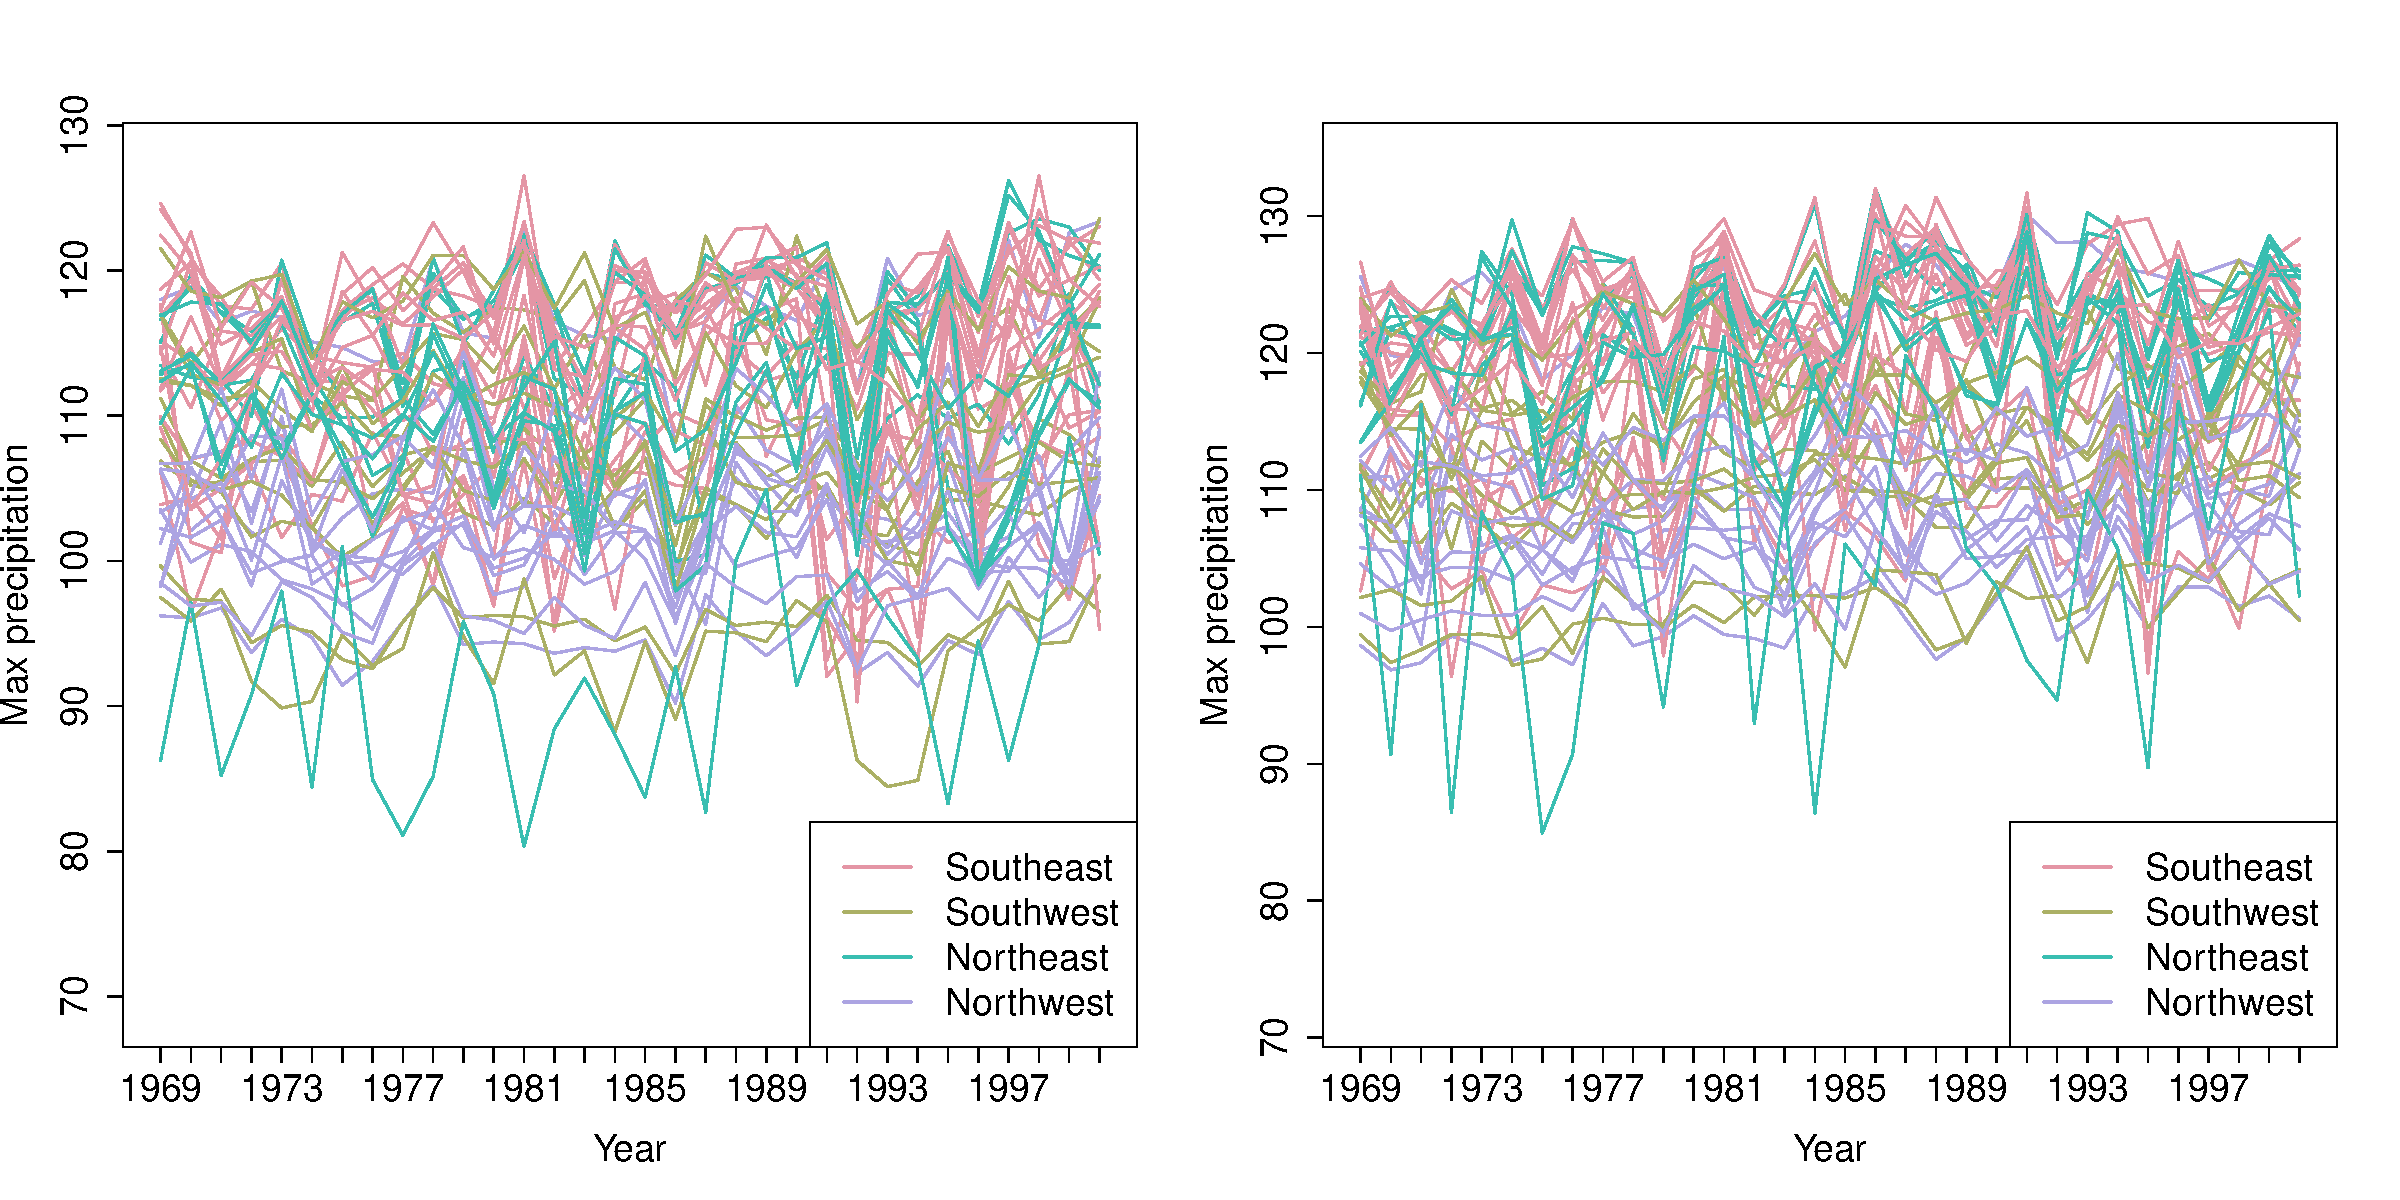
\includegraphics[width=\linewidth]{plots/precip-ts}
  \caption{Time series of yearly max precipitation for current (1969 -- 2000) (left). Time series of yearly max precipitation for future (2039 -- 2070) (right).}
  \label{ebfig:tsprecip}
\end{figure}

For this dataset, to estimate the EBFs, we use the combined current and future data.
The first six EBFs for the combined data along with the cumulative sum of the contributions for $v_1, \ldots, v_{25}$ are given in \fref{ebfig:precip-ebfpanel}.
\begin{figure}[htbp]  % markdown/precipitation/cv-setup.R
  \centering
  \includegraphics[width=\linewidth]{plots/precip-ebf-panel.pdf}\\
  \includegraphics[width=0.35\linewidth]{plots/precipv-25.pdf}
  \caption{First six EBFs for the combined precipitation data and the cumulative sum of contributions $v_1, \ldots, v_{25}$.}
  \label{ebfig:precip-ebfpanel}
\end{figure}
As a comparison, we provide the first six principal components of the fire data along with the cumulative sum of the first 25 eigenvalues in \aref{eba:pca}.
For the precipitation data, we run the MCMC for 25,000 iterations using a burnin period of 15,000 iterations.
We consider models fit with both EBF and GSK, and fit the model using $L = 5, 10, \ldots, 40$.
Timing for each setting of $L$ is given in \tref{ebtbl:precip-scores} for 1,000.
The timings are obtained using the same machine as for the fire analysis.

\subsection{Results for precipitation analysis}\label{ebs:results-precip}
We use 5-fold cross-validation to assess the predictive performance of a model.
For each method, we randomly select 80\% of the observations across counties and years to be used as a training set to fit the model.
The remaining 20\% of sites and years are withheld for testing model predictions.
As with the fire analysis, we use Brier scores and quantile scores to compare model performance.
The Brier and quantile scores for the current and future precipitation data analysis are given in \tref{ebtbl:precip-scores}.
For these data, we observe more variation in the scores across the number of basis functions and generally an advantage in using EBF over GSK.
This is in contrast to the fire analysis, and is likely due to the fact that the spatial dependence is estimated to be much stronger than for the fire analysis.
When using the EBFs, the estimate of residual dependence for the precipitation data is $\hat{\alpha} = 0.280$ ($\alpha = 1$ is residual independence).

Based on the cross-validation results, we run a full analysis using all of the data with $L = 25$ and EBF.
\fref{ebfig:precip-ebf-postpanel} gives posterior summaries for three quantities of interest.
Because we have two separate time periods, current and future, we look at the differences between the estimates for $\hat{\mu}$, $\log(\hat{\sigma})$, and $\hat{q}(0.90)$ between $t_1 = 2000$ and $t_2 = 2070$ where $\hat{\mu}$, $\log(\hat{\sigma})$, and $\hat{q}(0.90)$ are calculated as described in \sref{ebs:results-fire}.
We plot \mbox{$\Delta \mu = \hat{\mu}_{2070} - \hat{\mu}_{2000}$}, \mbox{$\Delta \log(\hat{\sigma}) = \log(\hat{\sigma})_{2070} - \log(\hat{\sigma})_{2000}$}, and \mbox{$\Delta Q90 = \hat{q}(0.90)_{2070} - \hat{q}(0.90)_{2000}$}, and the estimated probabilites that each are positive.

The results seem to suggest that the strength of extreme rain events will increases between 2000 and 2070 as well as greater variability in the northeast region of the U.S. as well as Ohio and parts of the south.
There very strong evidence to suggest that most of the eastern U.S. should expect to see an increase in the 10-year return level between 2000 and 2070.
Exceptions to this trend appear in southern parts of Alabama and Mississippi and regions on the border between South Carolina and Georgia which will likely experience a decrease in the 10-year return level.

\section{Discussion}\label{ebs:con}
In this paper we have proposed new empirical basis functions for a data-driven low-rank approximation to a max-stable process.
The basis functions provide researchers with an exploratory data analysis tool to explore maps of extremal dependence over space.
The functions can also be used as inputs to an MCMC algorithm for inference and predicitons over space.
The results from the data analysis provide evidence to suggest that in the presence of strong spatial dependence as with the precipitation data, the empirical basis functions show an improvement in quantile scores over using knots and standardized Gaussian kernel functions without an increase in the amount of time for computing.

We have used the EBF for exploratory analysis and Bayesian inference.
Another possibility is to use the methods to reduce the data under consideration from the actual responses to loadings $A_{kt}$.
That is, given the EBF, one could obtain estimates of the $A_{kt}$ using a separate maximum likelihood estimation for each time point.
Time series of the estimated $A_{kt}$ may be used as a fast and simple method to study large-scale spatiotemporal trends.

\begin{landscape}
\begin{table}[htbp]
\caption{Average Brier scores ($\times 100$), average quantile scores for $q(0.95)$ and $q(0.99)$, and time (in minutes) for 1,000 iterations for precipitation analysis.}
\label{ebtbl:precip-scores}
\footnotesize
\centering
  \begin{tabular}{cc c cc c cc c c c cc c cc c c}
  \toprule
  & && \multicolumn{7}{c}{Current} && \multicolumn{7}{c}{Future}  \\
  \cmidrule{4-10} \cmidrule{12-18}
  & && \multicolumn{2}{c}{BS ($\times 100$)} && \multicolumn{2}{c}{QS} && && \multicolumn{2}{c}{BS ($\times 100$)} && \multicolumn{2}{c}{QS} \\
  \cmidrule{4-5} \cmidrule{7-8} \cmidrule{12-13} \cmidrule{15-16}
  $L$ & Process & \phantom{a} & $q(0.95)$ & $q(0.99)$ & \phantom{a} & $q(0.95)$ & $q(0.99)$ & \phantom{a} & Time & \phantom{abc} & $q(0.95)$ & $q(0.99)$ & \phantom{a} & $q(0.95)$ & $q(0.99)$ & \phantom{a} &  Time \\
  \midrule
  5  & EBF && 3.813 & 1.098 && 0.740 & 0.203 && 5.80 && 3.357 & 1.112 && 0.738 & 0.209 && 5.82\\
         & GSK && 3.854 & 1.074 && 0.745 & 0.204 && 5.54 && 3.338 & 1.101 && 0.742 & 0.210 && 5.49\\
  \midrule
  10 & EBF && 3.680 & 1.063 && 0.698 & 0.192 && 6.54 && 3.148 & 1.067 && 0.687 & 0.198 && 6.51\\
         & GSK && 3.628 & 1.068 && 0.705 & 0.195 && 6.30 && 3.088 & 1.072 && 0.709 & 0.201 && 6.26\\
  \midrule
  15 & EBF && 3.505 & 1.065 && 0.668 & 0.187 && 7.27 && 3.101 & 1.095 && 0.661 & 0.189 && 7.22\\
         & GSK && 3.618 & 1.051 && 0.695 & 0.194 && 7.05 && 3.057 & 1.064 && 0.697 & 0.199 && 7.02\\
  \midrule
  20 & EBF && 3.400 & 1.026 && 0.651 & 0.182 && 8.14 && 3.101 & 1.087 && 0.649 & 0.189 && 8.11\\
         & GSK && 3.552 & 1.039 && 0.688 & 0.192 && 7.87 && 3.065 & 1.062 && 0.692 & 0.196 && 7.85\\
  \midrule
  25 & EBF && 3.463 & 1.058 && 0.650 & 0.182 && 9.00 && 3.003 & 1.113 && 0.637 & 0.185 && 8.98\\
         & GSK && 3.643 & 1.063 && 0.679 & 0.190 && 8.74 && 2.039 & 1.054 && 0.686 & 0.196 && 8.71\\
  \midrule
  30 & EBF && 3.455 & 1.038 && 0.646 & 0.182 && 9.89 && 2.956 & 1.073 && 0.630 & 0.182 && 9.88\\
         & GSK && 3.550 & 1.046 && 0.684 & 0.191 && 9/60 && 3.074 & 1.067 && 0.685 & 0.195 && 9.55\\
  \midrule
  35 & EBF && 3.471 & 1.065 && 0.649 & 0.183 && 10.79 && 3.036 & 1.114 && 0.645 & 0.189 && 10.79\\
         & GSK && 3.608 & 1.064 && 0.686 & 0.194 && 10.46 && 3.083 & 1.075 && 0.691 & 0.199 && 10.43\\
  \midrule
  40 & EBF && 3.551 & 1.114 && 0.652 & 0.184 && 11.70 && 3.050 & 1.131 && 0.645 & 0.189 && 11.66\\
         & GSK && 3.605 & 1.067 && 0.686 & 0.194 && 11.32 && 3.104 & 1.083 && 0.693 & 0.199 && 11.28\\
  \bottomrule
  \end{tabular}
\end{table}
\end{landscape}

% \begin{figure}[htbp]  % markdown/precipitation/combine-tables.R
%   \centering
%   \includegraphics[width=\linewidth]{plots/precip-bs.pdf}
%   \caption{Brier scores for $q(0.95)$ and $q(0.99)$ to compare EBF and GSK analysis of precipitation data for current (left) and future (right).}
%   \label{ebfig:precip-bs}
% \end{figure}

% \begin{figure}[htbp]  % markdown/precipitation/combine-tables.R
%   \centering
%   \includegraphics[width=\linewidth]{plots/precip-bs.pdf}
%   \caption{Quantile scores for $q(0.95)$ and $q(0.99)$ to compare EBF and GSK analysis of precipitation data for current (left) and future (right).}
%   \label{ebfig:precip-qs}
% \end{figure}

\begin{figure}[htbp]  % markdown/precipitation/posterior_map.R
  \centering
  \includegraphics[height=0.9\textheight]{plots/precip-ebf-postpanel.pdf}
  \caption{Posterior mean of $\Delta \mu$ (top left), posterior mean of $\Delta \log(\sigma)$ (middle left), estimate of $\Delta Q90$ (bottom left), P$[\Delta \mu > 0]$ (top right), P$[\Delta \log(\sigma) > 0]$ (middle right), and P$[\Delta Q90 > 0]$ between 2000 and 2070 for precipitation data using EBF.}
  \label{ebfig:precip-ebf-postpanel}
\end{figure}

% \begin{figure}[htbp]  % markdown/precipitation/posterior_map.R
%   \centering
%   \includegraphics[width=\linewidth]{plots/precip-gsk-post-betatime.pdf}
%   \caption{Posterior mean of $\beta_{1, \text{time}}$ (left) and $\beta_{2, \text{time}}$ (right) for current (top) and future (bottom) precipitation data using GSK.}
%   \label{ebfig:fire-gskpostbeta1}
% \end{figure}

% \begin{figure}[htbp]  % markdown/precipitation/posterior_map.R
%   \centering
%   \includegraphics[width=\linewidth]{plots/precip-ebf-post-betatimepos.pdf}
%   \caption{Posterior P$(\beta_{1, \text{time}} > 0)$ (left) and P$(\beta_{2, \text{time}} > 0)$ (right) for current (top) and future (bottom) precipitation data using EBF.}
%   \label{ebfig:fire-ebfpostbeta1pos}
% \end{figure}

% \begin{figure}[htbp]  % markdown/precipitation/posterior_map.R
%   \centering
%   \includegraphics[width=\linewidth]{plots/precip-gsk-post-betatimepos.pdf}
%   \caption{Posterior P$(\beta_{1, \text{time}} > 0)$ (left) and P$(\beta_{2, \text{time}} > 0)$ (right) for current (top) and future (bottom) precipitation data using GSK.}
%   \label{ebfig:fire-gskpostbeta1pos}
% \end{figure}


% \begin{figure}[htbp]  % markdown/precipitation/posterior_map.R
%   \centering
%   \includegraphics[width=\linewidth]{plots/precip-q90diff-compare.pdf}
%   \caption{Difference in $q(0.90)$ for precipitation data between 2000 and 1969 for current (top) and 2070 and 2039 for future (bottom) using EBF (left) and GSK (right).}
%   \label{ebfig:precip-q90diff}
% \end{figure}

% \begin{figure}  % markdown/precipitation/combine-tables.R
%   \centering
%   \includegraphics[width=\linewidth]{plots/precip-bs.pdf}
%   \caption{Brier scores for current and future precipitation analysis.}
%   \label{ebfig:precip-bs}
% \end{figure}

% \begin{figure}  % markdown/precipitation/combine-tables.R
%   \centering
%   \includegraphics[width=\linewidth]{plots/precip-qs.pdf}
%   \caption{Quantile scores for current and future precipitation analysis.}
%   \label{ebfig:precip-qs}
% \end{figure}

% \begin{figure}  % markdown/precipitation/combine-tables.R
%   \centering
%   \includegraphics[width=\linewidth]{plots/precip-post-time.pdf}
%   \caption{Posterior distributions for $\beta_{\text{time}}$ for $\mu$ (left) and $\log(\sigma)$ (right).}
%   \label{ebfig:precip-qs}
% \end{figure}


%\include{Chapter-5/Chapter-5}
%\include{Chapter-6/Chapter-6}
%\restoregeometry


%%---------------------------------------------------------------------------%%
%%  Bibliography

%%  You can use the bibitem list.
%\bibliographystyle{unsrt}
%\begin{%thebibliography}{99}
%\bibitem{cb02}
%Casella, G. and Berger, R.L. (2002)
%\newblock {\it Statistical Inference, Second Edition.}
%Duxbury Press, Belmont, CA.
%
%\bibitem{t06}
%Tsiatis, A.A. (2006)
%\newblock {\it Semiparametric Theory and Missing Data.}
%Springer, New York.
%
%\end{thebibliography}

%% or use BibTeX
%\bibliography{Ortiz-thesis}{}
%\bibliographystyle{plain}
%\nociterec{*}

%\bibliographystyle{plainnat}%plainnat is necessary to enable the use of citet. Natbib style file.
%\bibliography{Ortiz-thesis2}
%\ensureoddstart
\begin{spacing}{1}
 \setlength\bibitemsep{11pt} %22pt = 2*11pt, where fontsize is 11pt
 \addcontentsline{toc}{chapter}{{\uppercase{\bibname}}} %\textorpdfstring and \uppercase needed due to hyperref package http://www.latex-community.org/forum/viewtopic.php?f=44&t=16601
 %\vspace{-0.5in}
\titleformat{\chapter}[display]{\bf\filcenter
}{\chaptertitlename\ \thechapter}{11pt}{\bf\filcenter}
\titlespacing*{\chapter}{0pt}{-0.5in-9pt}{22pt}

\printbibliography[heading=myheading]
\end{spacing}
%\bibliographystyle{apalike}


%%---------------------------------------------------------------------------%%
% Appendices
%\ensureoddstart
\restoregeometry
\appendix
\newgeometry{margin=1in,lmargin=1.25in,footskip=\chapterfootskip, includehead, includefoot}

\graphicspath{{./Chapter-2/}}
\chapter{A Space-time \Skewt Model for Threshold Exceedances}
\chaptermark{Space-time \Skewt Model}
\label{appendix:a}

\section{MCMC details} \label{sta:mcmc}
The MCMC sampling for the model in \sref{sts:hier} is done using {\tt R} (http://www.r-project.org). Whenever possible, we select conjugate priors (see \aref{sta:posterior}); however, for some of the parameters, no conjugate prior distributions exist.
For these parameters, we use a random walk Metropolis-Hastings update step.
In each Metropolis-Hastings update, we tune the algorithm during the burn-in period to give acceptance rates near 0.40.

\subsection*{Spatial knot locations}
For each day, we update the spatial knot locations, $\bw_1, \ldots, \bw_K$, using a Metropolis-Hastings block update.
Because the spatial domain is bounded, we generate candidate knots using the transformed knots $\bw^*_1, \ldots, \bw^*_K$ (see \sref{sts:temporal}) and a random walk bivariate Gaussian candidate distribution
\begin{align*}
  {\bw^*_k}^{(c)} \sim \text{N}({\bw^*_k}^{(r - 1)}, s^2 I_2)
\end{align*}
where ${\bw^*_k}^{(r - 1)}$ is the location for the transformed knot at MCMC iteration $r - 1$, $s$ is a tuning parameter, and $I_2$ is an identity matrix.
Let $\bY_t = [Y(\bs_1), \ldots, Y(\bs_n)]$ be the vector of observed responses at each site for day $t$.
After candidates have been generated for all $K$ knots, the acceptance ratio is
\begin{align*}
  R = \left\{ \frac{ l\left[ \bY_t | \bw_1^{(c)}, \ldots, \bw_K^{(c)}, \ldots\right] }{l\left[ \bY_t | \bw_1^{(r - 1)}, \ldots, \bw_K^{(r - 1)}, \ldots\right]} \right\} \times \left\{ \frac{ \prod_{k = 1}^{K}\phi\left(\bw_k^{(c)}\right)}{ \prod_{k = 1}^{K}\phi\left(\bw_k^{(r - 1)}\right)} \right\} \times \left\{ \frac{ \prod_{k = 1}^{K} p\left({\bw^*_k}^{(c)}\right)}{ \prod_{k = 1}^{K} p\left({\bw^*_k}^{(r - 1)}\right)}\right\}
\end{align*}
where $l$ is the likelihood given in \eref{steq:hier}, and $p(\cdot)$ is the prior either taken from the time series (see \sref{sts:temporal}) or assumed to be uniform over $\calD$.
The candidate knots are accepted with probability $\min\{R, 1\}$.

\subsection*{Spatial random effects}
If there is no temporal dependence amongst the observations, we use a Gibbs update for $z_{tk}$, and the posterior distribution is given in \aref{sta:posterior}.
If there is temporal dependence amongst the observations, then we update $z_{tk}$ using a Metropolis-Hastings update.
Because this model uses $|z_{tk}|$, we generate candidate random effects using the $z^*_{tk}$ (see \sref{sts:temporal}) and a random walk Gaussian candidate distribution
\begin{align*}
  {z^*_{tk}}^{(c)} \sim \text{N}({z^*_{tk}}^{(r - 1)}, s^2)
\end{align*}
where ${z^*_{tk}}^{(r-1)}$ is the value at MCMC iteration $r - 1$, and $s$ is a tuning parameter.
The acceptance ratio is
\begin{align*}
  R = \left\{ \frac{ l\left[\bY_t | z_{tk}^{(c)}, \ldots\right] }{ l\left[\bY_t | z_{tk}^{(r - 1)}\right]} \right\} \times \left\{ \frac{ p\left[ z_{tk}^{(c)} \right] }{ p\left[ z_{tk}^{(r - 1)}\right]}\right\}
\end{align*}
where $p[\cdot]$ is the prior taken from the time series given in \sref{sts:temporal}.
The candidate is accepted with probability $\min\{R, 1\}$.

\subsection*{Variance terms}
When there is more than one site in a partition, then we update $\sigma^2_{tk}$ using a Metropolis-Hastings update.
First, we generate a candidate for $\sigma^2_{tk}$ using an IG$(a^*/s, b^*/s)$ candidate distribution in an independence Metropolis-Hastings update where $a^* = (n_{tk} + 1) / 2 + a$, $b^* = \left[\bY_{tk}^\top \Sigma^{-1}_{tk} \bY_{tk} + z_{tk}^2\right] / 2 + b$, $n_{tk}$ is the number of sites in partition $k$ on day $t$, and $\bY_{tk}$ and $\Sigma^{-1}_{tk}$ are the observations and precision matrix for partition $k$ on day $t$.
The acceptance ratio is
\begin{align*}
  R = \left\{
    \frac{ l\left[\bY_t | {\sigma^2_{tk}}^{(c)}, \ldots\right] }
         { l\left[\bY_t | {\sigma^2_{tk}}^{(r - 1)}\right]}
    \right\} \times \left\{
    \frac{ l\left[z_{tk} | {\sigma^2_{tk}}^{(c)}, \ldots\right] }
         { l\left[z_{tk} | {\sigma^2_{tk}}^{(r - 1)}, \ldots\right] }
    \right\} \times \left\{
    \frac{ p\left[ {\sigma^2_{tk}}^{(c)} \right] }
         { p\left[ {\sigma^2_{tk}}^{(r - 1)}\right] }
    \right\} \times \left\{
    \frac{ c\left[ {\sigma^2_{tk}}^{(r - 1)}\right] }
         { c\left[ {\sigma^2_{tk}}^{(c)}\right]}
    \right\}
\end{align*}
where $p[\cdot]$ is the prior either taken from the time series given in \sref{sts:temporal} or assumed to be IG$(a, b)$, and $c[\cdot]$ is the candidate distribution.
The candidate is accepted with probability $\min\{R, 1\}$.

\subsection*{Spatial covariance parameters}
We update the three spatial covariance parameters, $\log(\rho)$, $\log(\nu)$, $\gamma$, using a Metropolis-Hastings block update step.
First, we generate a candidate using a random walk Gaussian candidate distribution
\begin{align*}
  \log(\rho)^{(c)} \sim \text{N}\left(\log(\rho)^{(r - 1)}, s^2\right)
\end{align*}
where $\log(\rho)^{(r-1)}$ is the value at MCMC iteration $r - 1$, and $s$ is a tuning parameter.
Candidates are generated for $\log(\nu)$ and $\gamma$ in a similar fashion.
The acceptance ratio is
\begin{align*}
  R = \left\{ \frac{ \prod_{t = 1}^{n_t} l \left[Y_t(\bs) | \rho^{(c)}, \nu^{(c)}, \gamma^{(c)}, \ldots \right] }{\prod_{t = 1}^{n_t} l \left[Y_t(\bs) | \rho^{(r-1)}, \nu^{(r-1)}, \gamma^{(r-1)}, \ldots \right] } \right\} \times \left\{ \frac{ p \left[\rho^{(c)} \right] }{ p \left[\rho^{(r - 1)}\right] } \right\} \times \left\{ \frac{ p \left[\nu^{(c)} \right] }{ p \left[\nu^{(r - 1)} \right] } \right\} \times \left\{ \frac{ p \left[ \gamma^{(c)} \right] }{ p \left[\gamma^{(r - 1)} \right] } \right\}.
\end{align*}
All three candidates are accepted with probability $\min\{R, 1\}$.

\section{Posterior distributions} \label{sta:posterior}

\subsection*{Conditional posterior of $z_{tk} \mid \ldots $}\label{sts:mvcondu}
If knots are independent over days, then the conditional posterior distribution of $|z_{tk}|$ is conjugate.
For simplicity, drop the subscript $t$, let $\tilde{z}_{k} = |z_{k}|$, $\tilde{\bz}_{k^c}$ be the vector of $[|z(\bs_1)|, \ldots, |z(\bs_n)|]$ for $\bs \notin P_k$, $\bX = [\bX(\bs_1), \ldots, \bX(\bs_n)]^\top$, let $\bY_k$ and $\bX_k$ be the observations and covariate measurements for $\bs \in P_k$, and let $\bY_{k^c}$ and $\bX_{k^c}$ be the observations and covariate measurements for $\bs \notin P_k$ and define
\begin{align*}
\bR = \begin{cases}
        \bY_k - \bX_k \bbeta & \bs \in P_k\\
        \bY_{k^c} - \bX_{k^c} \bbeta - \lambda \tilde{\bz}_{k^c} \qquad & \bs \notin P_k
        \end{cases}
\end{align*}
Let
\begin{align*}
    \bR_1 &= \text{the vector of } \bR \text{ for } \bs \in P_k \\
    \bR_2 &= \text{the vector of } \bR \text{ for } \bs \notin P_k \\
    \Omega &= \Sigma^{-1}.
\end{align*}
Then
\begin{align*}
    \pi(z_k | \ldots) &\propto \exp \left\{ -\frac{ 1 }{ 2 } \left[
        \left( \begin{array}{c}
            \bR_1 - \lambda \tilde{z}_k \bOne\\
            \bR_2
        \end{array} \right)^\top
        \left( \begin{array}{cc}
            \Omega_{11} & \Omega_{12}\\
            \Omega_{21} & \Omega_{22}
        \end{array} \right)
        \left( \begin{array}{c}
            \bR_1 - \lambda \tilde{z}_k \bOne\\
            \bR_2
        \end{array} \right)
        +  \frac{ {\tilde{z}_k}^2 }{ \sigma_k^2 }\right]
    \right\} I \left(z_k > 0 \right) \\
        &\propto \exp \left\{ -\frac{ 1 }{ 2 } \left[ \Lambda_k {\tilde{z}_k}^2 - 2 \mu_k \tilde{z}_k \right] \right\}
\end{align*}
where
\begin{align*}
    \mu_k &= \lambda \left( \bR_1^\top \Omega_{11} + \bR_2^\top \Omega_{21} \right)\bOne\\
    \Lambda_k &= \lambda^2 \bOne^\top \Omega_{11} \bOne + \frac{ 1 }{ \sigma^2_k }.
\end{align*}
Then $\tilde{z}_k | \ldots \sim N_{(0, \infty)} \left(\Lambda_k^{-1} \mu_k, \Lambda_k^{-1} \right)$

\subsection*{Conditional posterior of $\bbeta, \lambda \mid \ldots$}\label{sts:betapost}
For models that do not include a skewness parameter, we update $\bbeta$ as follows.
Let $\bbeta \sim \mbox{N}_{p}(0, \Lambda_0)$ where $\Lambda_0$ is a precision matrix.
Then
\begin{align*}
    \pi(\bbeta \mid \ldots) & \propto \exp \left\{ - \frac{ 1 }{ 2 } \bbeta^\top \Lambda_0 \bbeta - \frac{ 1 }{ 2 } \sum_{t = 1}^{n_t} [\bY_t -\bX_t \bbeta]^\top \Omega [\bY_t - \bX_t \bbeta] \right\} \\
     & \propto \exp \left\{ -\frac{ 1 }{ 2 } \left[ \bbeta^\top \Lambda_\beta \bbeta  - 2 \sum_{t = 1}^{n_t} \left(\bbeta^\top \bX_t^\top \Omega \bY_t \right) \right] \right\} \\
     & \propto N_p ( \Lambda_\beta^{-1} \bmu_\beta , \bLambda_\beta^{-1})
\end{align*}
where
\begin{align*}
    \bmu_\beta &= \sum_{t = 1}^{n_t} \bX_t^\top \Omega \bY_t \\
    \bLambda_\beta &= \bLambda_0 + \sum_{t = 1}^{n_t} \bX_t^\top \Omega \bX_t.
\end{align*}
For models that do include a skewness parameter, a simple augmentation of the covariate matrix $\bX$ and parameter vector $\bbeta$ allows for a block update of both $\bbeta$ and $\lambda$.
Let $\bX^*_{t} = [\bX_t, |\bz_{t}|]$ where $\bz_t = [z(\bs_1), \ldots, z(\bs_{n})]^\top$ and let $\bbeta^* = (\beta_1, \ldots, \beta_p, \lambda)^\top$.
So to incorporate the $N(0, \sigma^2_\lambda)$ prior on $\lambda$, let $\bbeta^* \sim N_{p+1}(0, \Lambda^*_0)$ where
\begin{align*}
  \bLambda^*_0 = \left( \begin{array}{cc}
    \bLambda_0 & 0 \\
    0         & \sigma^{-2}_\lambda
  \end{array}\right).
\end{align*}
Then the update for both $\bbeta$ and $\lambda$ is done using the conjugate prior given above with $\bX_t = \bX_t^*$ and $\bbeta = \bbeta^*$

\subsection*{Conditional posterior of $\sigma^2 \mid \ldots$}\label{sts:sigpost}
In the case where $L = 1$ and temporal dependence is negligible, then $\sigma^2$ has a conjugate posterior distribution.
Let $\sigma_t^2 \iid \mbox{IG}(\alpha_0 / 2, \beta_0 / 2)$. For simplicity, drop the subscript $t$. Then
\begin{align*}
    \pi(\sigma^2 \mid \ldots) & \propto (\sigma^2)^{ -\alpha_0 / 2 - 1 / 2 - n / 2 - 1} \exp \left\{ -\frac{\beta_0}{2\sigma^2} - \frac{ |z|^2 }{2 \sigma^2} - \frac{ (\bY - \bmu)^\top \Sigma^{-1} (\bY - \bmu) }{2 \sigma^2} \right\} \\
    & \propto (\sigma^2)^{ -(\alpha_0 - 1 - n) / 2 - 1} \exp \left\{ - \frac{ 1 }{ 2 \sigma^2 } \left[\beta_0 + |z|^2 + (\bY - \bmu)^\top \Sigma^{-1} (\bY - \bmu) \right] \right\} \\
    & \propto \mbox{IG} (\alpha^*, \beta^*)
\end{align*}
where
\begin{align*}
    \alpha^* &= \frac{\alpha_0 + 1 + n}{2} \\
    \beta^* &= \frac{1}{2} \left[ \beta_0 + |z|^2 + (\bY - \bmu)^\top \Sigma^{-1} (\bY - \bmu) \right].
\end{align*}
In the case that $K > 1$, a random walk Metropolis Hastings step will be used to update $\sigma^2_{kt}$.

\section{Proof that $\displaystyle \lim_{h \rightarrow \infty} \pi(h) = 0$} \label{sta:proofsamepartition}
Let $c$ be the midpoint of $\bs_1$ and $\bs_2$.
Define $A$ as the circle centered at $c$ with radius $h / 2$ where $h = ||\bs_1 - \bs_2||$ is the distance between sites $\bs_1$ and $\bs_2$.
Consider a homogeneous spatial Poisson process over $A$ with intensity $\lambda_{\mathrm{PP}}$, so that
\begin{align*}
  \mu_{\mathrm{PP}}(A) = \lambda_{\mathrm{PP}} |A| = \lambda_{\mathrm{PP}} \pi \left(\frac{h}{2}\right)^2 = \lambda_{\mathrm{PPA}}^* h^2.
\end{align*}
Consider a partition of $A$ into four regions, $B_1$, $B_2$, $R_1$, $R_2$ as seen in \fref{stfig:hpp}.
\begin{figure}
  \includegraphics[width=\linewidth]{plots/circles}
  \caption{Illustration of the partition of $A$.}
  \label{stfig:hpp}
\end{figure}
Let $N_i$ be the number of knots in $B_i$ and $L_i = l$ if $\bs_i \in P_l$ for $i = 1, 2$.
Then
\begin{align}
  P(L_1 \neq L_2) \ge P(N_1 > 0, N_2 > 0)
\end{align}
since knots in both $B_1$ and $B_2$ is sufficient, but not necessary, to ensure that $\bs_1$ and $\bs_2$ are in different partition sets.
By definition of a Poission process, $N_1$ and $N_2$ are independent and thus \mbox{$P(N_1 > 0, N_2 > 0) = P(N_1 > 0)^2$}, and
\begin{align}
  \mu_{\mathrm{PP}}(B_1) &= \lambda_{\mathrm{PP}} |B_1| = \lambda_{\mathrm{PP}} \frac{h^2}{4} \left(\frac{2 \pi}{3} - \frac{\sqrt{3}}{2} \right) \nonumber \\
       &= \lambda^*_{\mathrm{PPB1}} h^2.
\end{align}
So,
\begin{align}
  P(L_1 \neq L_2) \ge P(N_1 > 0)^2 = [1 - P(N_1 = 0)]^2 = [1 - \exp\left(-\lambda^*_{\mathrm{PPB1}} h^2\right)]^2
\end{align}
which goes to 1 as $h$ goes to infinity.

%Then $\bs_1$ and $\bs_2$ are in different partitions almost surely if two or more points are in $A$.
%Let $N(A)$ be the number of points in $A$, and let
%\begin{align*}
%  \mu(A) = \lambda_{PP} |A| = \lambda_{PP} \pi \left(\frac{h}{2}\right)^2 = \lambda_{PP}^* h^2.
%\end{align*}

%
%
%Then
%\begin{align*}
%  P[N(A) \ge 2] &= 1 - P[N(A) = 0] - P[N(A) = 1]\\
%                &= 1 - \exp\{-\lambda h^2\} - \lambda h^2 \exp\{-\lambda h^2\} \\
%                &= 1 - (1 + \lambda h^2) \exp\{-\lambda h^2\}
%\end{align*}
%which goes to one as $h \rightarrow \infty$.


% Let $N(A)$ be the number of knots in $A$.
% So,
% \begin{align*}
%   P[ N(A) = k] = \frac{ \mu(A)^k \exp\{ -\mu(A)\}}{k!}.
% \end{align*}
% Then for any finite $k$, $\lim_{h \rightarrow \infty} P[N(A) = k] = 0$ because $\lim_{h \rightarrow \infty} \mu(A) = \infty$.
% With each additional knot in $A$, the chance that $\bs_1$ and $\bs_2$ will be be in the same partition will decrease, because partition membership is defined by the closest knot to a site.
% Therefore, $\lim_{h \rightarrow \infty} \pi(h) = 0$.

% \subsection{Half-normal distribution}
% Let $u = |z|$ where $Z \sim N(\mu, \sigma^2)$.
% Specifically, we consider the case where $\mu = 0$. Then $U$ follows a half-normal distribution which we denote as $U \sim HN(0, 1)$, and the density is given by
% \begin{align}
%   f_U(u) = \frac{ \sqrt{2} }{ \sqrt{\pi \sigma^2} } \exp \left( - \frac{ u^2 }{ 2 \sigma^2 } \right) I(u > 0)
% \end{align}
% When $\mu = 0$, the half-normal distribution is also equivalent to a $N_{(0, \infty)}(0, \sigma^2)$ where $N_{(a, b)}(\mu, \sigma^2)$ represents a normal distribution with mean $\mu$ and standard deviation $\sigma$ that has been truncated below at $a$ and above at $b$.

\section{\Skewt distribution} \label{sta:skewt}
\subsection*{Univariate \skewt distribution}
We say that $Y$ follows a univariate extended \skewt distribution with location $\xi \in \mathbb{R}$, scale $\omega > 0$, skew parameter $\alpha \in \mathbb{R}$, and degrees of freedom $\nu$ if has distribution function
\begin{align}
  f_{\text{EST}}(y) = 2 f_T (z; \nu) F_T\left[ \alpha z \sqrt{ \frac{ \nu + 1 }{ \nu + z^2}}; \nu + 1 \right]
\end{align}
where $f_T(t; \nu)$ is a univariate Student's $t$ with $\nu$ degrees of freedom, $F_T(t; \nu) = P(T < t)$, and \hbox{$z = (y - \xi) / \omega$}.

\subsection*{Multivariate \skewt distribution}
If $\bZ \sim \text{ST}_d(0, \bar{\bOmega}, \balpha, \eta)$ is a $d$-dimensional \skewt distribution, and $\bY = \xi + \bomega \bZ$, where $\bomega = \text{diag}(\omega_1, \ldots, \omega_d)$, then the density of $Y$ at $y$ is
\begin{align}
  f_y(\by) = \det(\bomega)^{-1} f_z(\bz)
\end{align}
where
\begin{align}
  f_z(\bz) &= 2 t_d(\bz; \bar{\bOmega}, \eta) T \left[ \balpha^\top \bz \sqrt{ \frac{\eta + d}{\nu + Q(\bz)} }; \eta + d\right] \\
  \bz &= \bomega^{-1}(\by - \xi)
\end{align}
where $t_d(\bz; \bar{\bOmega}, \eta)$ is a $d$-dimensional Student's $t$-distribution with scale matrix $\bar{\bOmega}$ and degrees of freedom $\eta$, $Q(z) = \bz^\top \bar{\Omega}^{-1}\bz$ and $T(\cdot; \eta)$ denotes the univariate Student's $t$ distribution function with $\eta$ degrees of freedom \citep{Azzalini2014}.

\subsection*{Extremal dependence}
For a bivariate \skewt random variable $\bY = [Y(\bs), Y(\bt)]^\top$, the $\chi(h)$ statistic \citep{Padoan2011} is given by
\begin{align} \label{steq:chiskew-t}
  \chi(h) = \bar{F}_{\text{EST}}\left\{ \frac{[x_1^{1 / \eta} - \varrho(h)] \sqrt{\eta + 1} }{\sqrt{1 - \varrho(h)^2}}; 0, 1, \alpha_1, \tau_1, \eta + 1 \right\} + \bar{F}_{\text{EST}}\left\{ \frac{ [x_2^{1 / \eta} - \varrho(h)] \sqrt{\eta + 1} }{ \sqrt{1 - \varrho(h)^2} }; 0, 1, \alpha_2, \tau_2, \eta + 1 \right\},
\end{align}
where $\bar{F}_{\text{EST}}$ is the univariate survival extended \skewt function with zero location and unit scale,
\begin{align*}
  \varrho(h) &= \text{Cor}[y(\bs), y(\bt)]\\
  \alpha_j &= \alpha_i \sqrt{1 - \varrho^2}\\
  \tau_j &= \sqrt{\eta + 1}(\alpha_j + \alpha_i \varrho)\\
  x_j &= \displaystyle\frac{F_T(\bar{\alpha}_i \sqrt{\eta + 1}; 0, 1, \eta)}{F_T(\bar{\alpha}_j \sqrt{\eta + 1}; 0, 1, \eta)},
\end{align*}
with $j = 1, 2$ and $i = 2, 1$ and where $\bar{\alpha}_j = (\alpha_j + \alpha_i \varrho) / \sqrt{ 1 + \alpha_i^2 [1 - \varrho(h)^2]}$.

\subsection*{Proof that $\displaystyle \lim_{h \rightarrow \infty} \chi(h) > 0$}
Consider the bivariate distribution of $\bY = [Y(\bs), Y(\bt)]^\top$, with $\varrho(h)$ given by \eref{steq:matern}.
So, $\displaystyle \lim_{h \rightarrow \infty} \varrho(h) = 0$.
Then
\begin{align}
  \lim_{h \rightarrow \infty} \chi(h) = \bar{F}_{\text{EST}}\left\{ \sqrt{\eta + 1}; 0, 1, \alpha_1, \tau_1, \eta + 1 \right\} + \bar{F}_{\text{EST}}\left\{ \sqrt{\eta + 1}; 0, 1, \alpha_2, \tau_2, \eta + 1 \right\}.
\end{align}
Because the extended \skewt distribution is not bounded above, for all $\bar{F}_{\text{EST}}(x) = 1 - F_{\text{EST} (x)} > 0$ for all $x < \infty$.
Therefore, for a \skewt distribution, $\displaystyle \lim_{h \rightarrow \infty} \chi(h) > 0$.

\sectionmark{Other parameterizations}
\section{Comparisons with other parameterizations}

\label{sta:otherparams}
Various forms of multivariate skew-normal and \skewt distributions have been proposed in the literature.
In this section, we make a connection between our parameterization in \eref{steq:fullmodel} of the main text and another popular version.
\citet{Azzalini2014} and \citet{Beranger2016} define a skew-normal process as
\begin{align}
  \tilde{X}(\bs) = \tilde{\lambda}|z| + (1 - \tilde{\lambda}^2)^{1 / 2} v(\bs)
\end{align}
where $\tilde{\lambda} \in (-1, 1)$, $z \sim N(0, 1)$, and $v(\bs)$ is a Gaussian process with mean zero, variance one, and spatial correlation function $\rho$.
To extend this to the \skewt distribution, \citet{Azzalini2003} take $\tilde{Y}(\bs) = W\tilde{X}(\bs)$ where $W^{-2} \sim $ Gamma$(a / 2, a / 2)$.
Returning to the proposed parameterization (with $\bbeta = 0$), let $W^{-2} = \frac{b}{a}\sigma^{-2}$ so that \eref{steq:fullmodel} in the manuscript becomes
\begin{align}
  Y(\bs) = W \left[ \lambda \left(\frac{b}{a}\right)^{1 / 2} |z| + \left(\frac{b}{a}\right)^{1 / 2} v(\bs) \right].
\end{align}
Clearly setting $b / a = (1 - \tilde{\lambda}^2) > 0$, and $\lambda = \tilde{\lambda} / (1 - \tilde{\lambda}^2)^{1 / 2} \in (-\infty, \infty)$ resolves the difference in parameterizations.
We note that our parameterization has three parameters $(a, b, \lambda)$ compared to the two parameters of the alternative parameterization $(a, \tilde{\lambda})$.
Since we have assumed that both $v(\bs)$ and $z$ have unit scale, the additional $b$ parameter in our parameterization is required to control the precision.
% However, if we introduce an overall scale parameter $c > 0$ into the alternative parameterization so that $\tilde{Y}(\bs) = c W \tilde{X}(\bs)$, then the two models remain equivalent by setting $a = \nu$, $b = \frac{\nu}{c^2 (1 - \tilde{\lambda}^2)}$, and $\lambda = \tilde{\lambda} / (1 - \tilde{\lambda}^2)^{1 / 2}$.

\section{Temporal dependence} \label{sta:temporal}
It is very challenging to derive an analytical expression the temporal extremal dependence at a single site $\bs$.
However, using simulated data, we have evidence to suggest that the model does exhibits temporal extremal dependence.
To demonstrate that our model maintains temporal extremal dependence, we generate lag-$m$ observations for $m = 1, 3, 5, 10$ from our model setting $\phi_w = \phi_z = \phi_\sigma = \varphi$, for $\varphi = 0, 0.02, 0.04, \ldots, 1$.
To estimate the lag-$m$ chi-statistic $\chi(m)$ we first estimate the lag-$m$ $F$-madogram $\nu_F(m)$ \citep{Cooley2006} using $\hat{\nu}_F(m) = \displaystyle \frac{1}{2n} \sum_{i = 1}^n \left| \hat{F}(y_{0}) - \hat{F}(y_{m}) \right|$ where $\hat{F}(\cdot)$ represents an empirical CDF and $y_m$ is the lag-$m$ observation.
The $F$-madogram is related to the $\chi$ statistic as follows
\begin{align}
  \chi = 2 - \frac{1 + 2 \nu_F}{1 - 2 \nu_F}.
\end{align}
\fref{stfig:chiphi} suggests that the extremal dependence increases as $\varphi \rightarrow 1$, and that the extremal dependence decreases as $m$ increases.
\begin{figure}
  \centering
  \includegraphics[width=0.6\linewidth]{plots/chi-phi}
  \caption{Simulated lag-$m$ $\chi$ for varying levels of $\varphi$.}
  \label{stfig:chiphi}
\end{figure}

% \section{Generating from the max-stable model of \citet{Reich2012}} \label{sta:reichshaby}
% The max-stable model of \citet{Reich2012} uses the \citet{Smith1990} max-stable process with a nugget term that follows a GEV(1, $\alpha$, $\alpha$).
% The purpose of the nuggest is to address criticism of the Smith max-stable process as unrealistically smooth.
% To generate from the max-stable model of \citet{Reich2012}, we use Algorithm 1.2 given of \citet{Stephenson2003}.
% In step 1, we generate from the symmetric logistic distribution using the \texttt{rmevd} function in the \texttt{evd} package in \texttt{R} with dependence parameter 0.5 \citep{Stephenson2002}.
% The dependence parameter, is similar to $\gamma$ in that it controls the relative strength of the nugget effect, so a setting of $0.5$ should give moderate spatial dependence.
% For the asymmetry parameters, we introduce 144 spatial knots on a regular lattice in the square $[1, 9] \times [1, 9]$.
% One contraint for this model is that the asymmetry parameters must sum to 1, so we use standardized Gaussian kernels with bandwidth 1 as in \citet[equations (2.5) and (2.6)]{Reich2012}.

\section{Brier scores for ozone prediction} \label{sta:ozonesite}

Because typical ozone concentration varies throughout the US, we have included Brier scores for exceedance of the 99th quantile by site for two model fits (Gaussian and Symmetric-$t$, $K = $ 10 knots, $T = $ 75, time series) in \fref{stfig:bssite}.
As we can see in these plots, both models seem to perform similarly across the US with the poorest performance in California.
Other methods have similar Brier score maps to these.
\begin{figure}
  \centering
  \includegraphics[width=0.8\linewidth]{plots/bs-site}
  \caption{Map of Brier scores for Gaussian (top) vs Symmetric-$t$, $K = $ 10 knots, $T = $ 75, time series (bottom).}
  \label{stfig:bssite}
\end{figure}

\section{Simulation study results} \label{sta:pdiffs}

The following tables show the methods that have significantly different Brier scores when using a Wilcoxon-Nemenyi-McDonald-Thompson test.
In each column, different letters signify that the methods have significantly different Brier scores.
For example, there is significant evidence to suggest that method 1 and method 4 have different Brier scores at $q(0.90)$, whereas there is not significant evidence to suggest that method 1 and method 2 have different Brier scores at $q(0.90)$.
In each table group A represents the group with the lowest Brier scores.
Groups are significant with a familywise error rate of $\alpha = 0.05$.

\begin{table}[htbp]
  \centering
  \caption{Setting 1 -- Gaussian marginal, $K = 1$ knot}
  \label{sttbl:gaussim}
  \begin{tabular}{c c ccc c ccc c cccc c cc}
  \toprule
     Method & \phantom{a} & \multicolumn{3}{c}{$q(0.90)$} & \phantom{a} & \multicolumn{3}{c}{$q(0.95)$} & \phantom{a} & \multicolumn{4}{c}{$q(0.98)$} & \phantom{a} & \multicolumn{2}{c}{$q(0.99)$} \\
    \cmidrule{1-1} \cmidrule{3-5} \cmidrule{7-9} \cmidrule{11-14} \cmidrule{16-17}
    1 && A &   &   && A &   &   && A &   &   &   && A &   \\
    2 && A &   &   && A &   &   && A &   &   &   && A &   \\
    3 &&   & B &   &&   & B &   &&   &   & C &   && A &   \\
    4 && A &   &   && A &   &   && A & B &   &   && A &   \\
    5 &&   & B &   &&   & B &   &&   & B & C &   && A &   \\
    6 &&   &   & C &&   &   & C &&   &   &   & D &&   & B \\
    \bottomrule
  \end{tabular}
\end{table}

% \begin{table}[htbp]
%   \centering
%   \caption{Setting 2: Symmetric-$t$ marginal, $K = 1$ knot}
%   \label{tbl:t1k1sim}
%   \begin{tabular}{|l|cc|cccc|cccc|ccc|}
%     \cline{2-14}
%     \multicolumn{1}{c}{} & \multicolumn{2}{|c}{$q(0.90)$} & \multicolumn{4}{|c}{$q(0.95)$} & \multicolumn{4}{|c}{$q(0.98)$} & \multicolumn{3}{|c|}{$q(0.99)$} \\
%     \hline
%     Method 1 &   & B &   &   &   & D &   &   &   & D &   &   & C \\
%     \hline
%     Method 2 & A &   & A &   &   &   & A &   &   &   & A &   &   \\
%     \hline
%     Method 3 &   & B &   & B &   &   &   & B & C &   &   & B &   \\
%     \hline
%     Method 4 & A &   &   &   & C &   &   & B &   &   &   & B &   \\
%     \hline
%     Method 5 &   & B &   &   &   & D &   &   & C & D &   & B & C \\
%     \hline
%   \end{tabular}
% \end{table}

% \begin{table}[htbp]
%   \centering
%   \caption{Setting 3: Symmetric-$t$ marginal, $K = 5$ knots}
%   \label{tbl:gaussim}
%   \begin{tabular}{|l|cc|cc|cc|cc|}
%     \cline{2-9}
%     \multicolumn{1}{c}{} & \multicolumn{2}{|c}{$q(0.90)$} & \multicolumn{2}{|c}{$q(0.95)$} & \multicolumn{2}{|c}{$q(0.98)$} & \multicolumn{2}{|c|}{$q(0.99)$} \\
%     \hline
%     Method 1 &   & B &   & B &   & B &   & B \\
%     \hline
%     Method 2 &   & B &   & B &   & B &   & B \\
%     \hline
%     Method 3 &   & B &   & B &   & B & A & B \\
%     \hline
%     Method 4 & A &   & A &   & A &   & A &   \\
%     \hline
%     Method 5 &   & B &   & B & A & B & A & B \\
%     \hline
%   \end{tabular}
% \end{table}

\begin{table}[htbp]
  \centering
  \caption{Setting 2 -- \Skewt marginal, $K = 1$ knot}
  \label{sttbl:st1sim}
  \begin{tabular}{c c cccc c cccc c cccc c ccc}
  \toprule
    Method & \phantom{a} & \multicolumn{4}{c}{$q(0.90)$} & \phantom{a} & \multicolumn{4}{c}{$q(0.95)$} & \phantom{a} & \multicolumn{4}{c}{$q(0.98)$} & \phantom{a} & \multicolumn{3}{c}{$q(0.99)$} \\
    \cmidrule{1-1} \cmidrule{3-6} \cmidrule{8-11} \cmidrule{13-16} \cmidrule{18-20}
    1 &&   & B &   &   &&   & B &   &   &&   & B &   &   &&   & B &   \\
    2 && A &   &   &   && A &   &   &   && A &   &   &   && A &   &   \\
    3 && A & B &   &   && A & B &   &   && A & B &   &   && A & B &   \\
    4 && A & B &   &   && A & B &   &   && A & B &   &   && A & B &   \\
    5 &&   &   & C &   &&   &   & C &   &&   &   & C &   &&   &   & C \\
    6 &&   &   &   & D &&   &   &   & D &&   &   &   & D &&   &   & C \\
    \bottomrule
  \end{tabular}
\end{table}

\begin{table}[htbp]
  \centering
  \caption{Setting 3 -- \Skewt marginal, $K = 5$ knots}
  \label{sttbl:st5sim}
  \begin{tabular}{c c cccc c cccc c ccc c ccc}
  \toprule
    Method & \phantom{a} & \multicolumn{4}{c}{$q(0.90)$} & \phantom{a} & \multicolumn{4}{c}{$q(0.95)$} & \phantom{a} & \multicolumn{3}{c}{$q(0.98)$} & \phantom{a} & \multicolumn{3}{c}{$q(0.99)$} \\
    \cmidrule{1-1} \cmidrule{3-6} \cmidrule{8-11} \cmidrule{13-15} \cmidrule{17-19}
    1 &&   &   & C &   &&   &   & C &   &&   & B &   &&   & B &   \\
    2 &&   &   & C &   &&   &   & C &   &&   & B &   &&   & B &   \\
    3 &&   & B &   &   &&   & B &   &   && A &   &   && A &   &   \\
    4 && A &   &   &   && A &   &   &   && A &   &   && A &   &   \\
    5 && A &   &   &   && A &   &   &   && A &   &   && A &   &   \\
    6 &&   &   &   & D &&   &   &   & D &&   &   & C &&   &   & C \\
    \bottomrule
  \end{tabular}
\end{table}

\begin{table}[htbp]
  \centering
  \caption{Setting 4 -- Max-stable, Asymmetric logistic}
  \label{sttbl:mssim}
  \begin{tabular}{c c cccc c cccc c ccc c ccc}
  \toprule
    Method & \phantom{a} & \multicolumn{4}{c}{$q(0.90)$} & \phantom{a} & \multicolumn{4}{c}{$q(0.95)$} & \phantom{a} & \multicolumn{3}{c}{$q(0.98)$} & \phantom{a} & \multicolumn{3}{c}{$q(0.99)$} \\
    \cmidrule{1-1} \cmidrule{3-6} \cmidrule{8-11} \cmidrule{13-15} \cmidrule{17-19}
    1 && A & B &   &   &&   & B &   &   &&   & B &   &&   &   & C \\
    2 &&   & B &   &   &&   & B &   &   &&   & B &   &&   & B & C \\
    3 &&   &   & C & D &&   &   & C &   &&   & B &   &&   & B &   \\
    4 &&   &   &   & D &&   &   &   & D &&   &   & C &&   &   & C \\
    5 &&   &   & C &   &&   & B & C &   &&   & B &   &&   & B & C \\
    6 && A &   &   &   && A &   &   &   && A &   &   && A &   &   \\
    \bottomrule
  \end{tabular}
\end{table}

\begin{table}[htbp]
  \centering
  \caption{Setting 5 -- Max-stable, Brown-Resnick}
  \label{sttbl:transsim}
  \begin{tabular}{c c cccc c ccc c ccc c ccc}
  \toprule
    Method & \phantom{a} & \multicolumn{4}{c}{$q(0.90)$} & \phantom{a} & \multicolumn{3}{c}{$q(0.95)$} & \phantom{a} & \multicolumn{3}{c}{$q(0.98)$} & \phantom{a} & \multicolumn{3}{c}{$q(0.99)$} \\
    \cmidrule{1-1} \cmidrule{3-6} \cmidrule{8-10} \cmidrule{12-14} \cmidrule{16-18}
    1 &&   &   &   & D &&   &   & C &&   &   & C &&   &   & C \\
    2 &&   &   &   & D &&   &   & C &&   &   & C &&   &   & C \\
    3 && A & B &   &   && A &   &   && A & B &   &&   & B &   \\
    4 &&   &   & C &   &&   & B &   &&   & B &   &&   & B &   \\
    5 && A &   &   &   && A &   &   && A &   &   && A & B &   \\
    6 &&   & B & C &   && A &   &   && A &   &   && A &   &   \\
    \bottomrule
  \end{tabular}
\end{table}
\vspace{\fill}
\graphicspath{{./Chapter-3/}}
\chapter{Spatial Model for Rare Binary Events}
\chaptermark{Spatial Rare Binary}
\label{appendix:b}

\section{Binary regression using the GEV link} \label{rba:rarebinary}

Here, we provide a brief review of the the GEV link of \citet{Wang2010}.
Let $Y_i \in \{0, 1\}$, $i = 1, \ldots, n$ be a collection of i.i.d. binary responses.
It is assumed that $Y_i = I(z_i > 0)$ where $I(\cdot)$ is an indicator function, $z_i = [1 - \xi \bX_i \bbeta]^{1 / \xi}$ is a latent variable following a GEV$(1, 1, 1)$ distribution, $\bX_i$ is the associated $p$-vector of covariates with first element equal to one for the intercept, and $\bbeta$ is a $p$-vector of regression coefficients.
Then, $Y_i \ind$ Bern$(\pi_i)$ where $\pi_i= 1 - \exp \left( -\frac{ 1 }{ z_i } \right)$.


\section{Derivation of the likelihood} \label{rba:likelihoodderivation}

We use the hierarchical max-stable spatial model given by \citet{Reich2012}. If at each margin, $Z_i \sim $ GEV$(1,1,1)$, then $Z_i | \theta_i \ind $ GEV$(\theta, \alpha \theta, \alpha)$. We reorder the data such that $Y_1=\cdots=Y_K=1$, and $Y_{K+1} = \cdots = Y_n = 0$. Then the joint likelihood conditional on the random effect $\theta$ is

\begin{align} \label{rbeq:joint_cond}
  P(Y_1=y_1,\ldots,Y_n=y_n) =& \prod_{ i \le K } \left\{ 1 - \exp \left[ - \left( \frac{ \theta_i }{ z_i } \right)^{ 1/\alpha} \right] \right \} \prod_{ i > K } \exp \left[ -\left( \frac{ \theta_i }{ z_i } \right)^{1/\alpha} \right] \nonumber \\[0.5em]
    =& \exp \left[ -\sum_{ i = K+1}^{ n }\left( \frac{ \theta_i }{ z_i } \right)^{1/\alpha} \right] - \exp \left[ -\sum_{ i = K+1}^{ n }\left( \frac{ \theta_i }{ z_i } \right)^{1/\alpha} \right] \sum_{ i = 1}^{K} \exp\left[ -\left( \frac{ \theta_i }{ z_i } \right)^{ 1/\alpha} \right] \nonumber\\
    &  + \exp \left[ -\sum_{ i = K+1}^{ n }\left( \frac{ \theta_i }{ z_i } \right)^{1/\alpha} \right] \sum_{ 1 < i < j \le K }  \exp \left[ - \left( \frac{ \theta_i }{ z_i } \right)^{ 1/\alpha} - \left( \frac{ \theta_j }{ z_j } \right)^{ 1/\alpha } \right] \nonumber \\[0.5em]
    & + \cdots + (-1)^K \exp\left[ - \sum_{ i = 1 }^{ n }\left( \frac{ \theta_i }{ z_i } \right)^{ 1/\alpha} \right]
\end{align}

Finally marginalizing over the random effect, we obtain

\begin{align} \label{rbeq:joint}
    P(Y_1=y_1,\ldots,Y_n=y_n) =&\int G(\bz | \bA) p( \bA | \alpha) \dd \bA. \nonumber\\[0.5em]
      =& \int \exp \left[ -\sum_{ i = K+1}^{ n }\left( \frac{ \theta_i }{ z_i } \right)^{1/\alpha} \right] - \exp \left[ -\sum_{ i = K+1}^{ n }\left( \frac{ \theta_i }{ z_i } \right)^{1/\alpha} \right] \sum_{ i = 1}^{K} \exp\left[ -\left( \frac{ \theta_i }{ z_i } \right)^{ 1/\alpha} \right] \nonumber\\
    &  + \exp \left[ -\sum_{ i = K+1}^{ n }\left( \frac{ \theta_i }{ z_i } \right)^{1/\alpha} \right] \sum_{ 1 < i < j \le K }  \exp \left[ - \left( \frac{ \theta_i }{ z_i } \right)^{ 1/\alpha} - \left( \frac{ \theta_j }{ z_j } \right)^{ 1/\alpha } \right] \nonumber \\[0.5em]
    & + \cdots + (-1)^K \exp\left[ - \sum_{ i = 1 }^{ n }\left( \frac{ \theta_i }{ z_i } \right)^{ 1/\alpha} \right] p( \bA | \alpha) \dd \bA.
\end{align}

Consider the first term in the summation,

\begin{align}
  \int \exp \left\{ -\sum_{ i = K+1}^{ n }\left( \frac{ \theta_i }{ z_i } \right)^{1/\alpha} \right\} p( \bA | \alpha) \dd \bA &= \int \exp \left\{ - \sum_{ i = K + 1 }^n \left( \frac{ \left[ \sum_{ l = 1 }^L  A_l w_{l}(\bs_i)^{1/\alpha} \right)^\alpha }{ z_i} \right]^{ 1/\alpha } \right \} p( \bA | \alpha) \dd \bA \nonumber \\[0.5em]
   &= \int \exp \left\{ -\sum_{ i = K + 1}^n \sum_{ l = 1}^L A_l \left( \frac{ w_l (\bs_i) }{ z_i } \right)^{1/\alpha} \right \} p( \bA | \alpha) \dd \bA \nonumber \\[0.5em]
   &=\exp\left\{-\sum_{ l = 1}^L \left[ \sum_{ i = K + 1 }^n \left( \frac{ w_l(\bs_i)}{ z_i} \right)^{1/\alpha} \right]^\alpha \right\}.
\end{align}

The remaining terms in equation \eref{rbeq:joint} are straightforward to obtain, and after integrating out the random effect, the joint density for $K = 0, 1, 2$ is given by
\begin{align}\label{rbeq:pmf}
  P(Y_1=y_1,\ldots,Y_n=y_n) =  \begin{cases}
      G(\bz), & K=0 \\
      G(\bz_{(1)})-G(\bz), & K=1 \\
      G(\bz_{(12)})-G(\bz_{(1)})-G(\bz_{(2)})+G(\bz), & K=2
    \end{cases}
\end{align}
where
\begin{align*}
  G[\bz_{(1)}] &= P[Z(\bs_2)<z(\bs_2),\ldots,Z(\bs_n)<z(\bs_n)] \\
  G[\bz_{(2)}] &= P[Z(\bs_1)<z(\bs_1),Z(\bs_3)<z(\bs_3),\ldots,Z(\bs_n)<z(\bs_n)]\\
  G[\bz_{(12)}] &= P[Z(\bs_3)<z(\bs_3),\ldots,Z(\bs_n)<z(\bs_n)].
\end{align*}
Similar expressions can be derived for all $K$, but become cumbersome for large $K$.

% \subsection{Proof that $\lim_{\beta \rightarrow \infty} \kappa(\beta) = \chi$} \label{rba:chi}
% Assume that $Z_1$ and $Z_2$ are both GEV$(\beta, 1, 1)$ so that the probability of $Y_i$ decreases to zero as $\beta$ increases.
% Recall from \sref{rbs:spatdep} that
% \begin{align*}
%   P_A(\beta) &= 1 - 2 \exp\left\{ -\frac{1}{\beta} \right\} + 2 \exp\left\{-\frac{\vartheta(\bs_1, \bs_2)}{\beta}  \right\} \\
%   P_E(\beta) &= 1 - 2 \exp \left\{ -\frac{1}{\beta} \right\} + 2 \exp \left\{ -\frac{2}{\beta} \right\}.
% \end{align*}
% Then
% \begin{align} \label{rbeq:kappabeta}
%   \kappa(\beta) &= \frac{P_A(\beta) - P_E(\beta)}{1 - P_E(\beta)} = \frac{\exp\left\{-\frac{\vartheta(\bs_1, \bs_2) - 1}{\beta}  \right\} - \exp \left\{ -\frac{1}{\beta} \right\}}{1 - \exp \left\{ -\frac{1}{\beta} \right\}}.
% \end{align}
% where $\vartheta(\bs_1, \bs_2)$ is defined as in \sref{rbs:spatdep}.
% So,
% \begin{align}
%   \kappa =
% \end{align}

% \subsection{Simulation study pairwise difference results} \label{rba:pdiffs}
% \hl{Needs updating}

% The following tables show the methods that have significantly different Brier scores when using a Wilcoxon-Nemenyi-McDonald-Thompson test.
% In each column, different letters signify that the methods have significantly different Brier scores.

% \begin{table}[htbp]
%   \centering
%   \caption{Pairwise BS comparisons}
%   \label{rbtbl:pwbssim}
%   \begin{tabular}{|l|cc|cc|c|ccc|cc|cc|}
%   \cline{2-13}
%   \multicolumn{1}{c}{} & \multicolumn{2}{|c}{Setting 1} & \multicolumn{2}{|c}{Setting 2} & \multicolumn{1}{|c}{Setting 3} & \multicolumn{3}{|c}{Setting 4} & \multicolumn{2}{|c}{Setting 5} & \multicolumn{2}{|c|}{Setting 6}\\
%   \hline
%   Method 1 & A &   & A &   & A &   &   & C &   & B &   & B \\
%   \hline
%   Method 2 & A & B &   & B & A &   & B &   & A &   & A &   \\
%   \hline
%   Method 3 &   & B &   & B & A & A &   &   & A & B & A &   \\
%   \hline
%   \end{tabular}
% \end{table}

% \begin{table}[htbp]
%   \centering
%   \caption{Pairwise AUC comparisons}
%   \label{rbtbl:pwaucsim}
%   \begin{tabular}{|l|cc|}
%   \multicolumn{1}{c}{} & \multicolumn{2}{|c}{Setting 1} \\
%   \hline
%   Method 1 & A &   & A &   \\
%   \hline
%   Method 2 & A & B & A & B \\
%   \hline
%   Method 3 &   & B &   & B \\
%   \hline
%   \end{tabular}
% \end{table}
\graphicspath{{./Chapter-4/}}
\chapter{Empirical Basis Functions for Max-stable Spatial Dependence}
\chaptermark{Empirical Basis Functions}
\label{appendix:c}

\section{Extreme value distributions} \label{eba:GEV}
The cumulative distribution function for the GEV is $F(y) = \exp\{-t(y)\}$ where
\begin{align} \label{ebeq:gevt}
  t(y) = \begin{cases}
      \left[1 + \xi \displaystyle \frac{y - \mu}{\sigma}\right]^{-1 / \xi}, \quad &\xi \neq 0 \\
      \\
      \exp\left\{- \displaystyle \frac{y - \mu}{\sigma}\right\}, &\xi = 0.
  \end{cases}
\end{align}
The probability density function for the GEV is given by $f(y) = \displaystyle \frac{1}{\sigma} t(x)^{\xi + 1} \exp\{-t(y)\}$ where $t(y)$ is defined in \eref{ebeq:gevt}.

\section{Grid approximation to PS density} \label{eba:gridapprox}
The PS($\alpha$) density can be challenging to use because it does not have a closed form.
From Section 2 of \citep{Stephenson2009}, the density can be expressed as
\begin{align}
  g_1(A) = \int_0^1 g_1(A, B) \dd B,
\end{align}
where
\begin{align}
  g_1(A, B) = \frac{\alpha}{1 - \alpha} \left( \frac{1}{A} \right)^{1 / 1 - \alpha} c(\pi B) \exp \left\{ -\left(\frac{1}{A}\right)^{\alpha / (1 - \alpha)} c(\pi B) \right\},
\end{align}
with
\begin{align}
  c(\psi) = \left[\frac{\sin(\alpha \psi)}{\sin(\psi)}\right]^{1 / (1 - \alpha)} \frac{\sin[(1 - \alpha) \psi]}{\sin(\alpha \psi)}.
\end{align}
\Citet{Stephenson2009} presents an auxiliary variable technique to deal with the integral in the density function, but we opt to numerically evaluate the integral because it is only one-dimensional.
To evaluate the integral, we use 50 evenly spaced quantiles of a Beta$(0.5, 0.5)$ distribution as the midpoints $B_1, \ldots, B_{50}$, and then use the midpoint rule to evaluate $\displaystyle \int_0^1 g_1(A, B) \dd B$.

\section{Standardized Gaussian kernel functions} \label{eba:gskfunctions}
\citet{Reich2012} use standardized Gaussian kernel functions as their spatial basis functions in the low-rank max-stable model.
Consider a set of $\bk_1, \ldots, \bk_L$ spatial knot locations in $\calD^2$, the region of interest.
Then
\begin{align}
  \hat{B}_{il} = \frac{\exp\left\{- \displaystyle\frac{||\bs_i - \bk_l||^2}{2 \rho^2} \right\}}{\displaystyle \sum_{j = 1}^L \exp\left\{- \frac{||\bs_i - \bk_j||^2}{2 \rho^2} \right\}}
\end{align}
where $|| \cdot ||$ is the Euclidean distance between a site and a knot location.

\section{Principal components} \label{eba:pca}
As a comparison to the EBFs, \fref{ebfig:fire-eigpanel} gives the first six principal components for the fire data, and \fref{ebfig:precip-eigpanel} gives the first six principal components for the precipitation data.
These figures show that the EBFs resemble the EOFs  for the uncersored precipitation data, but are quite different that the EOF from the censored fire data.
This is not surprising considering that the censoring results in only a small subset of data being used to estimate dependence.
\begin{figure}[htbp] % markdown/fire-analysis/basis-functions.R
  \centering
  \includegraphics[width=\linewidth]{plots/fire-eig-panel.pdf}

  \includegraphics[width=0.35\linewidth]{plots/firelambda-25.pdf}
  \caption{First six principal components and the cumulative sum of the first 25 eigenvalues for the Georgia fire data.}
  \label{ebfig:fire-eigpanel}
\end{figure}

% \begin{figure}[htbp] % markdown/fire-analysis/basis-functions.R
%   \centering
%   \includegraphics[width=0.5\linewidth]{plots/firelambda-25.pdf}
%   \caption{Cumulative sum of the first 25 eigenvalues.}
%   \label{ebfig:fire-eigpanel}
% \end{figure}

\begin{figure}[htbp]  % markdown/precipitation/cv-setup.R
  \centering
  \includegraphics[width=\linewidth]{plots/precip-eig-panel.pdf}

  \includegraphics[width=0.35\linewidth]{plots/preciplambda-25.pdf}
  \caption{First six principal components and the cumulative sum of the first 25 eigenvalues for the precipitation data.}
  \label{ebfig:precip-eigpanel}
\end{figure}
\restoregeometry

%%---------------------------------------------------------------------------%%
%\ensureoddstart
\backmatter


\end{document}
